\section{Introduction}
\label{sec:fourier-introduction}
Comme annoncé dans le chapitre \ref{chap:introduction}, une cuve
d'électrolyse typique dans une halle de production n'est jamais dans
un état stationnaire \cite{Steiner2009}, \cite{Flotron2013}. La cause
majeure pour laquelle ces cuves se trouvent dans un état de
déséquilibre constant est due aux changements d'anodes en fin de vie,
qui interviennent toutes les 24 heures environ.

Cet état de déséquilibre entraîne d'importantes variation des
écoulements des fluides dans la cuve, et ces variations ont un impact
non négligeable sur la répartition de l'alumine dissoute dans le bain
électrolytique. Pour palier à ces variations de répartition d'alumine,
les opérateurs peuvent modifier les cadences d'injection de chaque
injecteur. Malheureusement, il ne disposent pour l'heure d'aucun outil
qui leur permette de déterminer comment adapter ces cadences en
fonction de l'état de la cuve.

Le modèle de dissolution et transport d'alumine proposé dans
\cite{Hofer2011} et dont nous avons étudié certaines extensions dans
la première partie de ce travail, offre un début de réponse: la
conductivité des différentes anodes dépend de leur âge, ce qui modifie
le champs de vitesse dans le bain électrolytique et dans l'aluminium
liquide, ainsi que la distribution d'alumine
dissoute. Malheureusement, ce calcul ne peut pas être fait en temps
réel, et donc la cadence des injecteurs qui optimise la répartition de
l'alumine dissoute dans le bain ne peut pas non plus être obtenu en
temps réel.

Dans ce chapitre nous proposons une méthode pour calculer le champ de
vitesse dans une cuve d'électrolyse bien plus rapidement qu'avec les
modèles de \cite{Steiner2009} et \cite{Hofer2011}, au prix de
certaines hypothèses supplémentaires que l'on discutera.

La géométrie d'une cuve d'aluminium est particulier: l'essentiel de
l'écoulement des fluides prend place dans un domaine
parallélépipédique qui présente une forte anisotropie. Les dimensions
horizontales ($\approx \num{14}\times\num{4}$ \si{\meter}) sont bien plus
grandes que la dimension verticales ($\approx \num{0.2}$ \si{\meter}). Par
conséquent, l'écoulement est essentiellement contraint dans le plan
horizontal, si l'on néglige ce qui se passe dans les canaux bien
entendu.

Le modèle de référence dans Alucell \cite{Steiner2009},
\cite{Flotron2013}, \cite{Hofer2011}, \cite{Rochat2016} calcule une
approximation des écoulements dans les fluides en utilisant une
méthode d'éléments finis Lagrange continu linéaire par morceau sur un
maillage en tétraèdre du domaine fluide.

Or, la géométrie anisotrope du domaine fluide d'une cuve d'électrolyse
pose de sérieuses difficultés au niveau numérique. En effet,
l'utilisation de mailles isotropes n'est pas possible puisque la
taille de maille dans la direction verticale est de l'ordre de
\num{0.01} \si{\meter}.

La seule alternative est de considérer des mailles anisotropes ed
l'ordre de \num{0.01} \si{\meter} dans la direction verticale et
\num{0.1} \si{\meter} dans les directions horizontales.

Cependant, l'utilisation de mailles anisotropes augmente le
conditionnement des matrices et donc le nombre d'itérations
nécessaires à la résolution du système linéaire et dégrade la
précision du calcul.

Le but de ce chapitre est de proposer une méthode pour calculer des
écoulements de Stokes ou de Navier-Stokes dans des domaines
parallélépipédiques présentant une forte anisotropie. Dans la section
\ref{sec:fourier-model} nous proposons une décomposition de Fourier de la
vitesse selon la direction verticale, puis nous proposerons dans la
section \ref{sec:fourier-discretisation} une méthode numérique de type éléments
finis pour approcher chaque harmonique de la décomposition de
Fourier. Dans la section \ref{sec:fourier-validation} nous validons
l'implémentation du schéma ainsi obtenu et étudions la convergence de
l'erreur par rapport à une solution non triviale. Finalement, dans la
section \ref{sec:fourier-application} nous appliquons cette méthode au
cas industriel d'une cuve d'électrolyse et évaluons les propriétés de
cette méthode.


\section{Formulation du modèle de Stokes Fourier}
\label{sec:fourier-model}
Soit $\Lambda$ un ouvert borné de $\mathbb R^2$ de bord Lipschitzien
$\partial\Lambda$. Soit $\thickness > 0$ un nombre réel donné
correspondant à la dimension verticale d'une cuve. On définit le
domaine de $\mathbb R^3$ correspondant à une simplification
géométrique de la cuve d'électrolyse
\begin{equation}\label{eq:domain}
  \Omega = \Lambda \times (0,\thickness).
\end{equation}
On suppose que le domaine $\Omega$ est occupé par l'électrolyte, un
fluide newtonien incompressible de viscosité tensorielle $\mu$. On suppose de plus
que le tenseur de viscosité est tel que:
\begin{itemize}
  \item $\mu$ est symétrique, \ie, $\mu_{ij} = \mu_{ji}$, $1\leq
    i,j\leq 3$,
  \item $\exists \chi_0 > 0$ tel que $\mu_{ij} > \chi_0$, $1\leq
    i,j\leq 3$,
    \item $\mu$ est indépendent de $x_3$.
\end{itemize}
Si $u$ est la
vitesse de l'écoulement, le tenseur des contraintes visqueuses dans le
fluide \cite{Landau1987} est donné par
\begin{equation}
  \stresstensor_{i,j}(u) = 2\electrolyteviscosity_{i,j}
  \straintensor_{i,j}(u),\quad i,j = 1,2,3.
\end{equation}
Ici on a noté $\straintensor$ le tenseur du taux de déformation du
fluide qui s'écrit en fonction de la vitesse d'écoulement $u$:
\begin{equation}
  \straintensor_{i,j}(u) = \frac{1}{2}\parent{\frac{\partial u_i}{\partial x_j} + \frac{\partial u_j}{\partial x_i}},\quad i,j = 1,2,3.
\end{equation}
Étant donné un champ de forces $f:\Omega\to \mathbb R^3$, on suppose
que la vitesse d'écoulement $u:\Omega \to \mathbb R^3$ et la pression
$p:\Omega \to \mathbb R$ du fluide satisfont le système de Stokes stationnaire
\begin{align}
  &- \div(\stresstensor(u)) + \nabla p = f,\label{eq:stokes-u}\\
  &\div \parent{u} = 0\label{eq:stokes-p}
\end{align}
dans $\Omega$. Dans la suite nous noterons $u = (u_1, u_2, u_3)$ et $f =
(f_1, f_2, f_3)$. De plus, on demande à ce que l'écoulement $u$ satisfasse
les conditions aux limites suivantes. Sur les faces latérales, la
vitesse satisfait la condition d'adhérence
\begin{equation}
  u = 0\quad \text{ sur } \quad\partial \Lambda\times(0,\thickness).\label{eq:stokes-bc-1}
\end{equation}
Sur les faces horizontales supérieures et inférieures, la vitesse
d'écoulement satisfait une condition de glissement total. On a
\begin{align}
  &u_3(x_1, x_2, x_3) = 0,\label{eq:stokes-bc-2}\\
  &\parent{\stresstensor(u)\cdot \nu}\cdot t_i = 0,\quad i = 1,2\label{eq:stokes-bc-3}
\end{align}
sur $\Lambda \times\cparent{0,\thickness}$, avec $t_1$, $t_2$ les deux
vecteurs tangents unités.
Les conditions (\ref{eq:stokes-bc-2}), (\ref{eq:stokes-bc-3})
correspondent à demander à ce que le fluide ne pénètre pas les faces
horizontales de $\partial\Omega$ et à ce que les contraintes
tangentielles sur ces faces soient nulles. En utilisant
(\ref{eq:stokes-bc-2}), la condition (\ref{eq:stokes-bc-3}) se réécrit
\begin{equation}
\frac{\partial u_1}{\partial x_3} + \frac{\partial u_3}{\partial x_1}
  = 0 \quad \text{et} \quad \frac{\partial u_2}{\partial x_3} + \frac{\partial u_3}{\partial x_2}
  = 0\quad \text{ sur }\quad\partial \Lambda \times\cparent{0,\thickness}.
\end{equation}

\paragraph{Décomposition en séries de Fourier}
Pour résoudre le système d'équations (\ref{eq:stokes-u}),
(\ref{eq:stokes-p}) avec les conditions aux limites (\ref{eq:stokes-bc-1}) à
(\ref{eq:stokes-bc-3}), on exprime les inconnues sous forme de séries
de Fourier dans la direction $x_3$. Soit le domaine $\Omega^+ = \Lambda
\times (-\thickness, \thickness)$, on définit les fonctions suivantes
$\forall (x_1, x_2, x_3)\in \Omega^+$:
\begin{align}
  & U_i(x_1, x_2, x_3) = \left\{
    \begin{array}{lll}
      u_i(x_1, x_2, x_3) &\text{ si } x_3 \geq 0,\\
      u_i(x_1, x_2, -x_3) &\text{ si } x_3 < 0,     & \quad i = 1,2,
    \end{array}
  \right.\label{eq:decomp-1}\\
  %
  & U_3(x_1, x_2, x_3) = \left\{
    \begin{array}{ll}
       u_3(x_1, x_2, x_3) &\text{ si } x_3 \geq 0,\\
      -u_3(x_1, x_2, -x_3) &\text{ si } x_3 < 0,
    \end{array}
  \right.\label{eq:decomp-2}\\
  %
  & P(x_1, x_2, x_3) = \left\{
    \begin{array}{ll}
      p(x_1, x_2, x_3) &\text{ si } x_3 \geq 0,\\
      p(x_1, x_2, -x_3) &\text{ si } x_3 < 0,
    \end{array}
  \right.\label{eq:decomp-3}\\
  %
  & F_i(x_1, x_2, x_3) = \left\{
    \begin{array}{lll}
      f_i(x_1, x_2, x_3) &\text{ si } x_3 \geq 0,\\
      f_i(x_1, x_2, -x_3) &\text{ si } x_3 < 0,     & \quad i = 1,2,
    \end{array}
  \right.\label{eq:decomp-4}\\
  %
  & F_3(x_1, x_2, x_3) = \left\{
    \begin{array}{ll}
      f_3(x_1, x_2, x_3) &\text{ si } x_3 \geq 0\\
     -f_3(x_1, x_2, -x_3) &\text{ si } x_3 < 0.
    \end{array}
  \right.\label{eq:decomp-5}
\end{align}
En vertu de (\ref{eq:stokes-bc-2}) et (\ref{eq:stokes-bc-3}), les
dérivées selon $x_3$ des fonctions $U_1$, $U_2$ et $U_3$ ainsi
définies ne présentent pas de masse de Dirac en $x_3 = 0$. La figure
\ref{fig:solution-periodique} représente schématiquement le
comportement et la régularité de ces fonctions de part et d'autre de
l'origine de l'axe $x_3$.

\begin{figure}
  \begin{center}
    \input{../media/fourier/solution-periodique/solution-periodique.pdf_tex}
    \caption{Représentation schématique de la réplication des fonction
    $u_i$, $i = 1,2,3$, $p$, et $f_i$, $i = 1,2,3$ sur l'intervalle
      $(0, -\thickness)$. En $x_3 = 0$, les fonctions $U_i$,
      $i=1,2,3$ sont $\mathcal C^1$, $P$, $F_1$, $F_2$ sont $\mathcal
      C^0$, et $F_3$ est discontinue.}
    \label{fig:solution-periodique}
  \end{center}
\end{figure}


Avec les définitions ci-dessus on vérifie que $U = (U_1, U_2, U_3)$ et
$P$ satisfont les équations
\begin{align}
  &-\div\parent{\mathcal T(U)} + \nabla P = F,\label{eq:stokes-periodic-1}\\
  &\div\parent{U} = 0\label{eq:stokes-periodic-2}
\end{align}
dans $\Omega^+$. De plus on a
\begin{equation}
U_3 = 0 \quad\text{ sur } \Lambda\times \cparent{-\thickness} \text{ et } \Lambda\times \cparent{\thickness}
\end{equation}
et
\begin{equation}
  \frac{\partial U_i}{\partial x_3} = 0\quad \text{ sur } \Lambda\times
  \cparent{-\thickness} \text{ et } \Lambda\times \cparent{\thickness}
\end{equation}
pour $i = 1,2$, c'est-à-dire que
\begin{equation}
\parent{\stresstensor(U)\cdot \nu}\cdot t_i = 0\quad i = 1,2, \text{ sur } \Lambda\times
\cparent{-\thickness, \thickness}.
\end{equation}

On prolonge toutes les fonctions dans la variable $x_3$ sur tout
$\mathbb R$ en des fonctions périodiques de période $2\thickness$ en
$x_3$. On note encore par $U_1$, $U_2$, $U_3$, $P$, $F_1$, $F_2$,
$F_3$ ces prolongements, c'est-à-dire que ces fonctions sont
considérées comme fonctions de $(x_1, x_2, x_3)\in \Lambda\times
\mathbb R$ et $2\thickness$-périodiques selon $x_3$. Les fonctions
$U_1$, $U_2$, $U_3$ sont $\mathcal C^2$ par morceaux, $P$ est
$\mathcal C^1$ par morceaux et $F_1$, $F_2$, $F_3$ sont $C^0$ par
morceaux.

On pose pour alléger l'écriture $\beta^k = \frac{\pi
k}{\thickness}$. Les décompositions en séries de Fourier selon la
variable $x_3$ des fonctions $U_i$, $F_i$, $i = 1,2,3$ et $P$ s'écrivent
\begin{align}
  &U_i(x_1, x_2, x_3) = u_i^0(x_1, x_2) %
                       + \sum_{k > 0} u_i^k(x_1, x_2)%
                       \cos\parent{\beta^kx_3}, &\quad i = 1, 2,\label{eq:fourier-coeff-def-1}\\
  &U_3(x_1, x_2, x_3) = \sum_{k > 0} u_3^k(x_1, x_2)%
                        \sin\parent{\beta^kx_3},\label{eq:fourier-coeff-def-2}\\
  &P(x_1, x_2, x_3) = p^0(x_1, x_2) %
                      + \sum_{k>0}p^k(x_1, x_2)%
                      \cos\parent{\beta^kx_3},\label{eq:fourier-coeff-def-3}\\
  &F_i(x_1, x_2, x_3) = f_i^0(x_1, x_2) %
                        + \sum_{k > 0}f_i^k(x_1, x_2)%
                        \cos\parent{\beta^kx_3}, &\quad i = 1,2,\label{eq:fourier-coeff-def-4}\\
  &F_3(x_1, x_2, x_3) = \sum_{k > 0}f_3^k(x_1,x_2)%
                        \sin\parent{\beta^kx_3}.\label{eq:fourier-coeff-def-5}
\end{align}
On note $u^0 = (u^0_1, u^0_2)$, $f^0 = (f^0_1, f^0_2)$, $u^k =
(u^k_1,u^k_2,u^k_3)$ et $f^k = (f^k_1, f^k_2, f^k_3)$, $k \geq 1$. On
obtient les équations que les coefficients de Fourier $u^k$, $p^k$,
$k>0$ doivent satisfaire en substituant les définitions
(\ref{eq:fourier-coeff-def-1}) à (\ref{eq:fourier-coeff-def-5}) dans
le système d'équation de Stokes
(\ref{eq:stokes-periodic-1}),(\ref{eq:stokes-periodic-2}). Les bases
de Fourier $\cparent{\cos(\beta^k x_3)}_{k > 0}$ et
$\cparent{\sin(\beta^kx_3)}_{k>0}$ sur $\mathbb R$ étant
respectivement orthogonales, on peut identifier les équations pour
chaque mode indépendamment des autres. On obtient pour $k = 0$:
\begin{align}
  &-\sum_{j = 1}^2\frac{\partial}{\partial
    x_j}\parent{\mu_{ji}\parent{\frac{\partial u_i^0}{\partial x_j} +
      \frac{\partial u_j^0}{\partial x_i}}} + \frac{\partial
    p^0}{\partial x_i} = f_i^0, \quad i = 1,2,\label{eq:fourier-fund-1}\\
  &\sum_{j = 1}^2 \frac{\partial u_j^0}{\partial x_j} = 0\label{eq:fourier-fund-2}
\end{align}
sur $\Lambda$ et $u^0 = 0$ sur $\partial \Lambda$.

On obtient pour $k
\geq 1$:
\begin{align}
  &-\sum_{j = 1}^2\frac{\partial}{\partial
    x_j}\parent{\mu_{ji}\parent{\frac{\partial u_i^k}{\partial x_j} +
      \frac{\partial u_j^k}{\partial x_i}}} -
  \mu_{3i}\parent{\beta^k\frac{\partial u_3^k}{\partial x_i} -
    \parent{\beta^k}^2 u_i^k} + \frac{\partial p^k}{\partial x_i} = f_i^k,\quad
  i = 1,2,\label{eq:fourier-harm-1}\\
  &-\sum_{j = 1}^2\frac{\partial}{\partial
    x_j}\parent{\mu_{j3}\parent{\frac{\partial u_3^k}{\partial x_j} -
      \beta^k u_j^k}} + 2\mu_{33}\parent{\beta^k}^2 u_3^k - \beta^k p^k =
  f_3^k,\label{eq:fourier-harm-2}\\
  &\sum_{j = 1}^2\frac{\partial u_j^k}{\partial x_j} + \beta^k u_3^k = 0\label{eq:fourier-harm-3}
\end{align}
sur $\Lambda$ et $u^k = 0$ sur $\partial \Lambda$.

Étant données les forces $F_i$, $i = 1,2,3$, les coefficients $f^k$,
$k \geq 0$ qui apparaissent dans les membres de droite des équations
(\ref{eq:fourier-fund-1}), (\ref{eq:fourier-harm-1}) et
(\ref{eq:fourier-harm-2}) s'obtiennent par une projection $\mathrm
L^2$ sur la base de Fourier correspondante. Pour $k = 0$ on a
\begin{align}
  f_i^0(x_1, x_2) &=
  \frac{1}{2\thickness}\int_{-\thickness}^{\thickness}F_i(x_1, x_2, x_3)\,\mathrm
  dx_3, \quad i = 1,2,\nonumber\\
  &= \frac{1}{\thickness}\int_{0}^{\thickness}f_i(x_1, x_2, x_3)\,\mathrm
  dx_3, \quad i = 1,2,\label{eq:f-1}
\end{align}
et pour $k > 0$ on a
\begin{align}
f_i^k(x_1, x_2) &=
\frac{1}{\thickness}\int_{-\thickness}^{\thickness}F_i(x_1, x_2,
x_3)\cos\parent{\beta^k x_3}\,\mathrm dx_3,\quad i =
1,2,\\
&=
\frac{2}{\thickness}\int_{0}^{\thickness}f_i(x_1, x_2,
x_3)\cos\parent{\beta^k x_3}\,\mathrm dx_3,\quad i =
1,2,\label{eq:f-2}\\
f_3^k(x_1, x_2) &= \frac{1}{\thickness}\int_{-\thickness}^{\thickness}
F_3(x_1, x_2,x_3) \sin\parent{\beta^k x_3}\,\mathrm
dx_3,\\
&= \frac{2}{\thickness}\int_{0}^{\thickness}
f_3(x_1, x_2,x_3) \sin\parent{\beta^k x_3}\,\mathrm
dx_3.\label{eq:f-3}
\end{align}


\paragraph{Formulation faible}\label{sec:stokes-fourier-weak}
Nous énonçons maintenant les formulations variationnelles du problème
formé par les équations (\ref{eq:fourier-fund-1}) et
(\ref{eq:fourier-fund-2}) qui correspondent au mode fondamental de
l'écoulement $u$, et des problèmes formés par les équations
(\ref{eq:fourier-harm-1}) à (\ref{eq:fourier-harm-3}) qui
correspondent à chacune des harmoniques de l'écoulement $u$. Pour ce
faire, nous aurons besoin des espaces fonctionnels suivants. L'espace
$L^2(\Lambda)$ est l'ensemble
\begin{align}
  L^2(\Lambda) = \cparent{f:\Lambda\to\mathbb R \mathrel{\Big|} \int_\Lambda
    \abs{f}^2\mathrm dx < \infty}.
\end{align}
Il est muni du produit scalaire
\begin{align}
  (f, g)_{L^2(\Lambda)} = \int_\Lambda f(x)g(x)\mathrm dx
\end{align}
pour tout $f, g\in L^2(\Lambda)$, et de la norme
\begin{align}
  \norm{f}_{L^2(\Lambda)} = \sqrt{(f, f)_{L^2(\Lambda)}}\quad\forall f\in L^2(\Lambda).
\end{align}
On notera encore $H^1(\Lambda)$ l'espace de Sobolev
$W^{1,2}(\Lambda)$, c'est-à-dire que
\begin{align}
  H^1(\Lambda) = \cparent{f\in L^2(\Lambda)\mathrel{\bigg|} \int_\Lambda
    \abs{\nabla f}^2 \mathrm dx < \infty}
\end{align}
et
\begin{align}
  H^1_0(\Lambda) = \cparent{f \in H^1(\Lambda) \mathrel{\bigg|}
    f|_{\partial \Lambda} = 0}.
\end{align}
Nous aurons finalement besoin des espaces de fonctions à moyenne nulle
\begin{align}
  &L^2_0(\Lambda) = \cparent{f\in L^2(\Lambda)\mathrel{\bigg|}
    \int_\Lambda f \,\mathrm dx = 0},\\
  \text{et }\quad &H^1_{0,0}(\Lambda) = \cparent{f\in H^1_0(\Lambda)\mathrel{\bigg|}
    \int_\Lambda f \,\mathrm dx = 0}.
\end{align}
Remarquons que $L^2_0(\Lambda)$ est un sous-espace fermé de
$L^2(\Lambda)$ et $H^1_{0,0}(\Lambda)$ est un sous-espace fermé de
$H^1_0(\Lambda)$ ce qui sera important pour répondre aux questions
d'existence et d'unicité par la suite.

Commençons tout d'abord par traiter le mode fondamental. Pour
simplifier l'écriture, on note $\overline{\mu}$ et
$\reducedstraintensor$ la viscosité et le tenseur du taux de
déformation réduits aux composantes 1 et 2:
\begin{equation}
 \overline{\mu} = \begin{bmatrix}
  \mu_{1,1} & \mu_{1,2} \\
  \mu_{2,1} & \mu_{2,2}
 \end{bmatrix},\quad \text{et} \quad \reducedstraintensor_{ij}(u) =
 \straintensor_{ij}(u),\ i,j = 1,2.
\end{equation}
Le problème faible correspondant aux équations
(\ref{eq:fourier-fund-1}) et (\ref{eq:fourier-fund-2}) consiste à
chercher les fonctions $u_1^0,u_2^0 \in H^1_0(\Lambda)$, $p^0 \in
L^2_0(\Lambda)$, telles que
\begin{align}
  &\int_\Lambda \electrolyteviscosity\otimes \reducedstraintensor(u^0) : \reducedstraintensor(v) \intd{x_1}\intd{x_2} -
  \int_\Lambda p^0\div v \intd{x_1}\intd{x_2} = \int_\Lambda f^0\cdot v
  \intd{x_1}\intd{x_2},\label{eq:fourier-weak-fund-1}\\
  &\int_\Lambda q\div u^0 \intd{x_1}\intd{x_2} = 0,\label{eq:fourier-weak-fund-2}
\end{align}
pour toutes fonctions $v \in \parent{H^1_0(\Lambda)}^2$, $q \in
L_0^2(\Lambda)$. Ici $\otimes$ est le produit tensoriel, \ie,
$\parent{\mu\otimes\reducedstraintensor}_{i,j} =
\mu_{ij}\reducedstraintensor_{ij}$ et $\mu\otimes\reducedstraintensor(u):\reducedstraintensor(v) =
\sum_{i,j = 1}^2\mu_{ij}\reducedstraintensor_{ij}(u)\reducedstraintensor_{ij}(v)$.
En admettant que $\partial \Lambda$ est Lipschitzien et en supposant
que $f^0\in \mathrm L^2(\Lambda)$, il est connu que la formulation
faible (\ref{eq:fourier-weak-fund-1}),(\ref{eq:fourier-weak-fund-2})
admet une unique solution \cite{Temam1977}.

Traitons à présent les problèmes pour les coefficients $u^k$ et
$p^k$. Soit $k > 0$ et soit $\tilde \straintensor^k$ le tenseur $3\times
3$ défini par
\begin{equation}
  \tilde\straintensor^k(u) = \begin{bmatrix}
     2\frac{\partial u_1}{\partial x_1}
    & \frac{\partial u_1}{\partial x_2} + \frac{\partial u_2}{\partial x_1}
    & \frac{\partial u_3}{\partial x_1} - \beta_k u_1 \\
    %
       \frac{\partial u_2}{\partial x_1} + \frac{\partial u_1}{\partial x_2}
    & 2\frac{\partial u_2}{\partial x_2}
    &  \frac{\partial u_3}{\partial x_2} - \beta_k u_2 \\
    %
       \frac{\partial u_3}{\partial x_1} - \beta_k u_1
    &  \frac{\partial u_3}{\partial x_2} - \beta_k u_2
    & 2\beta_k u_3
  \end{bmatrix}
\end{equation}
On obtient la formulation faible pour chaque harmonique en multipliant
les équations (\ref{eq:fourier-harm-1}) à (\ref{eq:fourier-harm-3})
par des fonctions test $v_1$, $v_2$, $v_3$ et $q$ et en intégrant par
parties les termes qui comportent des dérivées secondes. Le problème
faible pour chaque harmonique $k$ consiste à chercher les fonctions
$u^k = (u_1^k,u_2^k,u_3^k)\in \parent{H^1_0(\Lambda)}^3$ et $p^k\in
L^2(\Lambda)$ telles que
\begin{align}
  &\int_\Lambda 2\mu\otimes\tilde\straintensor^k(u^k):\tilde\straintensor^k(v)
  - \int_\Lambda p^k\parent{\frac{\partial v_1}{\partial x_1} +
    \frac{\partial v_2}{\partial x_2} + \beta^k v_3}
  = \int_\Lambda f^k\cdot v,\label{eq:fourier-weak-harm-1}\\
  &\int_\Lambda \parent{\frac{\partial u_1^k}{\partial x_1} + \frac{\partial u_2^k}{\partial x_2} + \beta^k u_3^k}q = 0\label{eq:fourier-weak-harm-2}
\end{align}
pour toutes fonctions $v = (v_1,v_2,v_3)\in \parent{H^1_0(\Lambda)}^3$
et $q\in L^2(\Lambda)$. Ici on adopte les mêmes notations que
précédemment pour le produit tensorielle avec $i,j =
1,2,3$. Remarquons que l'on omet $\intd{x_1}\intd{x_2}$ dans les
intégrales pour simplifier l'écriture. Nous reformulons maintenant ce
problème sous une forme plus adéquate pour l'analyse qui suit.  On
montre en utilisant le théorème de la divergence et en posant $\tilde
p^k = p^k - C^k$ avec $C^k = \abs{\Lambda}^{-1} \int_\Lambda
p^k\intd{x_1}\intd{x_2}$ que le problème
(\ref{eq:fourier-weak-harm-1}),(\ref{eq:fourier-weak-harm-2}) est
équivalent au problème suivant: trouver $u^k\in H^1_0(\Lambda)^3$,
$\tilde p^k \in L^2_0(\Lambda)$ et $C^k\in\mathbb R$ tels que pour
tout $v\in H^1_0(\Lambda)^3$ et $q \in L^2_0(\Lambda)$:
\begin{align}
  &\int_\Lambda 2\mu\otimes\tilde\straintensor^k(u^k):\tilde\straintensor^k(v)
  - \int_\Lambda \tilde p^k\parent{\frac{\partial v_1}{\partial x_1} +
    \frac{\partial v_2}{\partial x_2}} - \int_\Lambda(\tilde p^k +
  C^k)\beta^k v_3
  = \int_\Lambda f^k\cdot v,\label{eq:fourier-weak-harm-v2-1}\\
  &\int_\Lambda \parent{\frac{\partial u_1^k}{\partial x_1} +
    \frac{\partial u_2^k}{\partial x_2} + \beta^k u_3^k}q =
  0,\label{eq:fourier-weak-harm-v2-2}\\
  &\int_\Lambda u_3^k = 0.\label{eq:fourier-weak-harm-v2-3}
\end{align}
Soit maintenant $\psi \in H^1_0(\Lambda)$ tel que $\int_\Lambda
\psi\,\mathrm dx \neq 0$. Alors on peut écrire $H^1_0(\Lambda) =
H^1_{0,0}(\Lambda) \oplus W$, où $W =\mathrm{span}(\psi)$. En
cherchant $u_3^k \in H^1_{0,0}(\Lambda)$ (voir éq. (\ref{eq:fourier-weak-harm-v2-3})), on obtient
le problème que l'on montrera bien posé suivant: trouver $u^k \in
H_0^1(\Lambda)^2 \times H_{0,0}^1(\Lambda)$, $\tilde p^k \in
L^2_0(\Lambda)$ tels que pour tout $v \in H_0^1(\Lambda)^2 \times
H_{0,0}^1(\Lambda)$, $q \in L^2_0(\Lambda)$ on ait
\begin{align}
  &\int_\Lambda 2\mu\otimes\tilde\straintensor^k(u^k):\tilde\straintensor^k(v)
  - \int_\Lambda \tilde p^k\parent{\frac{\partial v_1}{\partial x_1} +
    \frac{\partial v_2}{\partial x_2} + \beta^k v_3}
  = \int_\Lambda f^k\cdot v,\label{eq:fourier-weak-harm-v3-1}\\
  &\int_\Lambda \parent{\frac{\partial u_1^k}{\partial x_1} + \frac{\partial u_2^k}{\partial x_2} + \beta^k u_3^k}q = 0\label{eq:fourier-weak-harm-v3-2}
\end{align}
La constante $C^k$ est unique et peut être calculée a posteriori en
connaissant les fonctions $u^k$ et $\tilde p^k$. Nous reportons la
discussion de ce point à la fin de cette section.

Afin de rendre plus explicite la structure sous-jacente de cette
formulation, on peut l'exprimer en des termes plus abstraits. Notons
$V = H^1_0(\Lambda)^2\times H^1_{0,0}(\Lambda)$. Soit $a^k:V\times V
\to \mathbb R$ les formes bilinéaires continues définies pour tout $k
> 0$ par
\begin{equation}
  a^k(u,v) = \int_\Lambda
  2\mu\otimes\tilde\straintensor^k(u):\tilde\straintensor^k(v)
\end{equation}
et les formes bilinéaires continues $b^k:V\times L^2_0(\Lambda)\to\mathbb
R$ définies pour tout $k > 0$ par
\begin{equation}
  b^k(u, q) = \int_\Lambda \parent{\frac{\partial u_1}{\partial x_1} +
    \frac{\partial u_2}{\partial x_2} + \beta^k u_3}q.
\end{equation}
Ainsi pour $k$ fixé, le problème (\ref{eq:fourier-weak-harm-v3-1}),
(\ref{eq:fourier-weak-harm-v3-2}) est équivalent au problème de
chercher $(u^k,\tilde p^k)\in V \times L^2_0(\Lambda)$ tel que
\begin{align}
  &a^k(u^k,v) - b^k(v,p^k) = \int_\Lambda f^k\cdot v,\label{eq:abstr-weak-harm-1}\\
  & b^k(u^k, q) = 0\label{eq:abstr-weak-harm-2}
\end{align}
pour tout $(v, q)\in V \times L^2_0(\Lambda)$.

\paragraph{Existence d'une solution faible pour les harmoniques}
On donne maintenant une preuve de l'existence et de l'unicité du
problème faible (\ref{eq:abstr-weak-harm-1}),
(\ref{eq:abstr-weak-harm-2}) pour chaque coefficient $(u^k,p^k)$. Dans ce
but, nous introduisons au préalable les deux lemmes suivants.

\begin{lemme}\label{lem:1}
Soit un entier $k > 0$ fixé et une fonction $u \in H^1_0(\Lambda)^3$
telle que $\frac{\partial u_1}{\partial x_1} + \frac{\partial
  u_2}{\partial x_2} + \beta^k u_3 = 0$. On a la relation
\begin{equation}
\int_\Lambda \abs{\tilde\straintensor^k(u)}^2 = \int_\Lambda
\parent{\abs{\reducedstraintensor(u)}^2 +
  \frac{1}{2}\parent{\parent{\frac{\partial u_3}{\partial x_1}}^2 +
    \parent{\frac{\partial u_3}{\partial x_2}}^2 +
    \parent{\beta^k u_1}^2  + \parent{\beta^k u_2}^2}}
\end{equation}
\end{lemme}

\begin{proof}
  Le calcul de $\abs{\tilde\straintensor^k(u)}^2$ une fois
  intégré sur $\Lambda$ donne:
  \begin{align}
    \int_\Lambda \abs{\tilde\straintensor^k(u)}^2 =
    &\int_\Lambda \parent{\abs{\reducedstraintensor(u)}^2
    + \frac{1}{2}\parent{
      \parent{\frac{\partial u_3}{\partial x_1}}^2
      + \parent{\frac{\partial u_3}{\partial x_2}}^2
      + \parent{\beta^k u_1}^2
      + \parent{\beta^k u_2}^2}}\nonumber\\
    &+ \int_\Lambda \beta^k\parent{
      - u_1 \frac{\partial u_3}{\partial x_1}
      - u_2 \frac{\partial u_3}{\partial x_2}
      + \beta^k\parent{u_3}^2
    }.\label{eq:lemme-inter-result}
  \end{align}
  Pour obtenir le résultat souhaité, il reste à voir que le
  dernier terme de (\ref{eq:lemme-inter-result}) est nul.
  En utilisant le théorème de la divergence et les conditions limites
  de $u_3$ sur $\partial \Lambda$ ($u_3 = 0$ sur $\partial \Lambda$) on obtient
  \begin{align}
    \int_\Lambda \beta^k\parent{
      - u_1 \frac{\partial u_3}{\partial x_1}
      - u_2 \frac{\partial u_3}{\partial x_2}
      + \beta^k\parent{u_3}^2} =
    \int_\Lambda\beta^k\parent{
        \frac{\partial u_1}{\partial x_1}u_3
      + \frac{\partial u_2}{\partial x_2}u_3 +
      \beta^k{u_3}^2}\label{eq:lemme-nul-term}
  \end{align}
  En utilisant l'hypothèse que $\frac{\partial u_1}{\partial x_1} +
  \frac{\partial u_2}{\partial x_2} + \beta^k u_3 = 0$ on obtient le
  résultat annoncé.
\end{proof}

\begin{lemme}\label{lem:2}
  Soit un entier $k > 0$ fixé. Il existe une constante positive $\chi >
  0$ telle que
  \begin{equation}
\chi \norm{\nabla u}_{L^2(\Lambda)} \leq
\norm{\tilde\straintensor^k(u)}_{L^2(\Lambda)},
  \end{equation}
  pour tout $u \in H^1_0(\Lambda)^3$ qui satisfait $\frac{\partial
    u_1}{\partial x_1} + \frac{\partial u_2}{\partial x_2} +
  \beta^k u_3 = 0$. Ici on a noté
  \begin{equation}
    \norm{\nabla u}_{L^2(\Lambda)}^2 = \sum_{i,j = 1}^3 \norm{\frac{\partial u_i}{\partial x_j}}^2_{L^2(\Lambda)}
  \end{equation}
  et
  \begin{equation}
    \norm{\tilde\straintensor(u)}^2_{L^2(\Lambda)} = \int_\Lambda \abs{\tilde\straintensor(u)}^2.
  \end{equation}
\end{lemme}

\begin{proof}
Il est connu que l'inégalité de Korn en dimension 2 est vraie, \ie, il
existe une constante $\chi > 0$ qui satisfait
\begin{equation}
\chi\sum_{i,j = 1}^2 \norm{\frac{\partial u_i}{\partial
    x_j}}^2_{L^2(\Lambda)} \leq \int_\Lambda \abs{\reducedstraintensor(u)}^2.
\end{equation}
Le lemme \ref{lem:1} permet de conclure.
\end{proof}

\begin{proposition}\label{prop:2}
  Si le tenseur de viscosité $\mu$ satisfait
\begin{equation}
  \mu_{i,j}(x_1,x_2) \geq \chi_0\quad \forall (x_1, x_2)\in \Lambda,\ 1
  \leq i,j \leq 3,\label{eq:hypothesis}
\end{equation}
où $\chi_0 > 0$ est une constante positive indépendante de $(x_1,
x_2)\in \Lambda$, alors le problème (\ref{eq:abstr-weak-harm-1}),
(\ref{eq:abstr-weak-harm-2}) admet une unique solution.
\end{proposition}

\begin{proof}
  Pour montrer la proposition \ref{prop:2}, il suffit de vérifier
  que la forme $a^k(.,.)$ est coercive sur $V_0$ où $V_0 = \cparent{v
    \in V\mid b^k(v, q) = 0\ \forall q \in
    L^2_0(\Lambda)}$, et que la condition classique inf-sup sur la forme
  bilinéaire $b^k$ est satisfaite.

  Montrons tout d'abord que $\frac{\partial u_1}{\partial x_1} +
  \frac{\partial u_2}{\partial x_2} + \parent{\beta^k}^2 u_3 = 0$,
  c'est-à-dire que
  \begin{equation}
    \int_\Omega\parent{\frac{\partial u_1}{\partial x_1} +
  \frac{\partial u_2}{\partial x_2} + \parent{\beta^k}^2 u_3}q =
    0,\quad \forall q\in L^2(\Lambda).
  \end{equation}
  Remarquons que
  \begin{equation}
    \int_\Omega\parent{\frac{\partial u_1}{\partial x_1} +
      \frac{\partial u_2}{\partial x_2} + \parent{\beta^k}^2 u_3}q =
    b^k(u, q),
  \end{equation}
  et on sait déjà que $b^k(u, q) = 0$ $\forall q \in
  L_0^2(\Lambda)$. De plus, on a que $b^k(u, q) = 0$ lorsque $q = 1$,
  puisque
  \begin{equation}
    \int_\Lambda u_3  = 0 \quad \text{et}\quad \int_\Lambda
    \frac{\partial u_1}{\partial x_1} + \frac{\partial u_2}{\partial
      x_2} = 0.
  \end{equation}

  Ainsi le lemme \ref{lem:1} s'applique, et les lemmes \ref{lem:1} et
  \ref{lem:2} avec l'hypothèse (\ref{eq:hypothesis}) montre bien que
  $a^k$ est coercive sur $V_0$. D'autre part en utilisant l'inégalité
  concernant la condition inf-sup dans $\mathbb R^2$ et si $q\in
  L^2_0(\Lambda)$, on a que
  \begin{align*}
    \sup_{\norm{v}_{H^1_0(\Lambda)^3} = 1} b^k(v,q) = &\sup_{\norm{v}_{H^1_0(\Lambda)^3} = 1} \int_{\Lambda}\parent{\frac{\partial v_1}{\partial x_1} + \frac{\partial v_2}{\partial x_2} + \beta^k v_3}q\\
    \geq & \sup_{\norm{(v_1, v_2, 0)}_{H^1_0(\Lambda)^3} =
      1}\int_{\Lambda}\parent{\frac{\partial v_1}{\partial x_1} +
      \frac{\partial v_2}{\partial x_2}}q\\
    = & \sup_{\norm{(v_1, v_2)}_{H^1_0(\Lambda)^2} = 1}\int_{\Lambda}\parent{\frac{\partial v_1}{\partial x_1} + \frac{\partial v_2}{\partial x_2}}q\\
    \geq& \gamma \norm{q}_{L^2_0(\Lambda)},
  \end{align*}
  où $\gamma > 0$. Ainsi on a bien
  \begin{equation*}
    \inf_{q\in L^2_0(\Lambda)}\sup_{v\in V} \frac{b(v,
      q)}{\norm{q}_{L^2_0(\Lambda)}\norm{v}_{V}} \geq \gamma > 0,
  \end{equation*}
  et la proposition est prouvée.
\end{proof}

Afin d'obtenir le coefficient de Fourier de la pression $p^k$, il
reste à calculer la constante $C^k$ et à montrer son unicité. En
prenant la fonction test $v = (0,0,\psi)$ dans
(\ref{eq:fourier-weak-harm-v2-1}) on obtient
\begin{align}
\int_\Lambda 2\mu\otimes
\tilde\straintensor^k(u^k):\tilde\straintensor^k(v) -
\beta^k\int_\Lambda (\tilde p^k + C^k) = \int_\Lambda f_3 \psi, \label{eq:fourier-pressure-constant}
\end{align}
ce qui permet de calculer $C^k$.

On montre enfin que le calcul de la constante $C^k$ ne dépend pas du
choix de la fonction de base $\psi$ de $W$. En effet, en considérant
une autre fonction $\phi \in H^1_0(\Lambda)$ telle que $\int_\Lambda
\phi \neq 0$ alors $\phi = \bar\phi + \tilde \phi$ où $\tilde \phi \in
H^1_{0,0}(\Lambda)$ et $\bar \phi \in W$ puisque $H^1_0(\Lambda) =
H^1_{0,0} \oplus W$. Cette décomposition implique qu'il existe une
unique constante $\gamma \in \mathbb R$ telle que $\bar \phi = \gamma
\psi$. Si, au lieu de $v = (0,0,\psi)$ on prend $v = (0,0,\phi) =
(0,0,\tilde \phi) + (0,0,\gamma \psi)$ dans
(\ref{eq:fourier-weak-harm-v2-1}), alors $(0,0,\tilde \phi) \in
H^1_0(\Lambda)^2\times H^1_{0,0}(\Lambda)$. Cette fonction test est
comprise dans (\ref{eq:fourier-weak-harm-v3-1}). D'autre part
$(0,0,\gamma \psi)$ donne la même constante $C^k$ que la relation
(\ref{eq:fourier-pressure-constant}).


\section{Discrétisation par une méthode d'éléments finis}
\label{sec:fourier-discretisation}
Dans cette section nous décrivons les méthodes de discrétisations
proposées pour approximer le coefficient du mode fondamental de
l'écoulement $(u^0, p^0)$ et les coefficients des harmoniques $(u^k,
p^k)$.

Soit un nombre réel $h > 0$ et soit $\mathcal M_h$ une triangulation
du domaine $\Lambda$ de $\mathbb R^2$ telle que $\diam(\meshcell)\leq h$,
$\forall \meshcell\in \mathcal M_h$. On introduit maintenant l'espace
éléments finis $V_h$ défini par
\begin{equation}
  V_h = \cparent{v\in C^0(\Lambda)\mid v|_\meshcell \in \mathbb
    P_1(\meshcell)\ \forall \meshcell\in\mathcal M_h},
\end{equation}
avec $\mathbb P_1(\meshcell)$ l'espace des polynômes de degré 1 sur le
triangle $\meshcell$. On définit aussi l'espace enrichi par une fonction bulle
\begin{equation}
  B_h = \cparent{v \in C^0(\Lambda)^2 \mid v|_\meshcell \in \mathbb P_1^2\oplus
    B_\meshcell\ \forall \meshcell\in\mathcal M_h} \cap H_0^1(\Lambda)^2
\end{equation}
où $B_\meshcell$ est engendré par la fonction $27 \lambda_1^\meshcell
\lambda_2^\meshcell\lambda_3^\meshcell$, les $\lambda_i^\meshcell$, $i = 1,2,3$, étant les
trois fonctions barycentriques du triangle $\meshcell$.

\paragraph{Mode fondamental}
La méthode d'éléments finis correspondant à la discrétisation des équations
(\ref{eq:fourier-weak-fund-1}), (\ref{eq:fourier-weak-fund-2})
consiste à chercher $(u^0_h, p^0_h)\in B_h\times(V_h \cap
L^2_0(\Lambda))$ tels que, pour tout $(v_h, q_h)\in
B_h\times(V_h \cap L^2_0(\Lambda))$ on ait
\begin{align}
  &\int_\Lambda
  2\mu\otimes\reducedstraintensor(u^0_h):\reducedstraintensor(v)
  -\int_\Lambda p^0_h\div(v_h) = \int_\Lambda f^0\cdot v_h, \label{eq:fourier-fund-discrete-1}\\
  & \int_\Lambda q_h\div u^0_h = 0.\label{eq:fourier-fund-discrete-2}
\end{align}
Il est connu que le couple d'espaces éléments finis $(B_h, V_h \cap
L^2_0(\Lambda))$ est stable, ainsi (\ref{eq:fourier-fund-discrete-1}),
(\ref{eq:fourier-fund-discrete-2}) admet une unique solution \cite{Temam1977}.

Le schéma (\ref{eq:fourier-fund-discrete-1}),
(\ref{eq:fourier-fund-discrete-2}) fait intervenir l'espace
éléments finis à moyenne nulle $V_h \cap L^2_0(\Lambda)$ pour le mode
fondamental de la pression $p^0$. En pratique, on exprime
explicitement la contrainte sur la pression dans le problème faible
en ajoutant l'équation
\begin{equation}
\int_\Lambda p^0_h = 0
\end{equation}
et en ajoutant un multiplicateur de Lagrange pour la fonction test $q_h$. Il est alors équivalent
de chercher $(u^0_h, p^0_h)\in B_h\times V_h$ et
$\lambda\in\mathbb R$ tels que, pour tout $(v_h, q_h)\in
B_h\times V_h$ on ait
\begin{align}
  &\int_\Lambda
  2\mu\otimes\reducedstraintensor(u^0_h):\reducedstraintensor(v)
  -\int_\Lambda p^0_h\div(v_h) = \int_\Lambda f^0\cdot v_h, \label{eq:fourier-fund-discrete-1-prat}\\
  & \int_\Lambda q_h\div u^0_h + \lambda \int_\Lambda q_h =
  0,\label{eq:fourier-fund-discrete-2-prat}\\
  & \int_\Lambda p_h^0 = 0.\label{eq:fourier-fund-discrete-3-prat}
\end{align}

\paragraph{Harmoniques}
On considère à présent la discrétisation de la formulation
faible (\ref{eq:fourier-weak-harm-1}),
(\ref{eq:fourier-weak-harm-2}). Pour $k > 0$ donné, le problème
discrétisé consiste à chercher les fonctions $(u^k_h, p^k_h) \in
(V_h\cap H_0^1(\Lambda))^3\times V_h$ telles que
\begin{align}
  &\int_\Lambda 2\mu\otimes
  \tilde\straintensor(u^k_h):\tilde\straintensor(v) - \int_\Lambda
  p_h^k\parent{\frac{\partial v_{1,h}}{\partial x_1}
    \frac{\partial v_{2,h}}{\partial x_2} +\beta^k p^k_h v_{3,h}} =
  \int_\Lambda f\cdot v_h,\label{eq:fourier-harm-discrete-1}\\
  &\int_\Lambda \parent{\frac{\partial u^k_{1,h}}{\partial x_1} +
    \frac{\partial u^k_{2,h}}{\partial x_2} + \beta^k u^k_{3,h}}q_h +
  \delta \sum_{\meshcell\in\mathcal M_h} h_\meshcell^2
  \int_\meshcell\parent{\parent{\beta^k}^2 p^k_h q_h + \nabla p_h^k \nabla
    q_h} = 0\label{eq:fourier-harm-discrete-2}
\end{align}
pour tout $(v_{1,h}, v_{3,h}, v_{3,h}, q_h) \in (V_h\cap
H_0^1(\Lambda))^3\times V_h$. Ici $\delta > 0$ et le terme de
stabilisation dans (\ref{eq:fourier-harm-discrete-2}) qui est justifié
par le fait que, d'après (\ref{eq:fourier-coeff-def-3}),
\begin{equation}
  \Delta P = \Delta p^0 + \sum_{k > 0} (\Delta p^k -
  \parent{\beta^k}^2 p^k)\cos(\beta^k x_3).
\end{equation}

\paragraph{Quadrature pour les coefficients de Fourier de la force}
En pratique, les forces $f_i$, $i = 1,2,3$ sont données aux sommets du
maillage $\mathcal M_h$. Les intégrales qui interviennent dans les
définitions (\ref{eq:f-1}), (\ref{eq:f-2}) et (\ref{eq:f-3}) sont
approchées par une formule de Simpson sur une subdivision uniforme de
l'intervalle $[0, \thickness]$. Le nombre de subdivision sera choisi
de sorte à ce que cette erreur de quadrature soit négligeable par
rapport aux erreurs introduites par les discrétisations éléments
finis et la troncature de la série de Fourier.

\paragraph{Résolution des systèmes linéaires}
Les systèmes linéaires issus des formulations
(\ref{eq:fourier-fund-discrete-1-prat})-(\ref{eq:fourier-fund-discrete-3-prat})
et(\ref{eq:fourier-harm-discrete-1}),(\ref{eq:fourier-harm-discrete-2})
sont résolus avec la méthode GMRES préconditionnée par ILU(2). Le
critère d'arrêt de l'itération de GMRES est:
\begin{equation}
  \frac{\norm{P^{-1}\parent{Ax^n - b}}_{l^2}}{\norm{P^{-1}\parent{Ax^0 - b}}_{l^2}} \leq \num{1e-10},
\end{equation}
où $A$ est la matrice associée à la forme bilinéaire d'une formulation
variationnelle, $P$ le préconditionneur ILU(2) associé à la matrice
$A$, $b$ le vecteur du membre de droite associé à la forme linéaire et
$x^n$ les valeurs de l'approximation de la solution $x$ aux itérations
successives de l'algorithme GMRES.

\paragraph{Reconstruction de la solution}
On se fixe un entier $K > 0$, on suppose avoir calculé $u^k$, $p^k$, $k
= 1, 2,\dots, K$ solutions de (\ref{eq:fourier-fund-discrete-1-prat})-%
(\ref{eq:fourier-fund-discrete-3-prat}) et
(\ref{eq:fourier-harm-discrete-1}),
(\ref{eq:fourier-harm-discrete-2}). En vertu de
(\ref{eq:fourier-coeff-def-1})-(\ref{eq:fourier-coeff-def-3}), on note
pour tout $(x_1, x_2, x_3)\in \Omega$
\begin{align}
  &u_{i,h,K}(x_1, x_2, x_3) = u_{i,h}^0(x_1, x_2) + \sum_{k = 1}^K
  u_{i,h}^k \cos\parent{\beta^k x_3},\quad i = 1,2\label{eq:u-h-12}\\
  &u_{3,h,K}(x_1, x_2, x_3) = \sum_{k = 1}^K
  u_{3,h}^k \sin\parent{\beta^k x_3}\label{eq:u-h-3}
\end{align}
et
\begin{align}
  p_{h,K}(x_1, x_2, x_3) = p_h^0(x_1, x_2) + \sum_{k = 1}^K p_h^k(x_1,
  x_2) \cos\parent{\beta^k x_3}.
\end{align}
Enfin on notera $u_{h,K} = (u_{1,h,K}, u_{2,h,K}, u_{3,h,K})$.


\section{Validation numérique}
\label{sec:fourier-validation}



\section{Modèle de transport d'alumine stationnaire}
\label{sec:fourier-alumina-model}
L'objectif ultime étant d'obtenir une approximation de la
concentration d'alumine dans la cuve, on propose un modèle de
transport et diffusion stationnaire d'alumine dissoute dans le domaine
$\Omega$.  On suppose donné un champ de convection stationnaire
$u:\Omega\to\mathbb R^3$, qui correspond à l'écoulement des fluides
dans le domaine $\Omega$. Le champ $u$ sera typiquement calculé à
l'aide du schéma numérique introduit dans la section
\ref{sec:fourier-discretisation}.  Soit $S$ le terme source de la
concentration d'alumine dissoute correspondant à l'injection de
particules, $\dot q$ le terme source correspondant à la consommation
d'alumine dissoute par la réaction d'électrolyse, et la diffusivité
moléculaire de la concentration d'alumine dans le bain $D_C^M > 0$.
On cherche le champ de concentration d'alumine stationnaire
$c:\Omega\to\mathbb R$ solution de l'équation d'advection-diffusion
\begin{equation}\label{eq:stat-concentration}
  u\cdot \nabla c - D_c^M \Delta c = S + \dot q\quad \text{dans } \Omega,
\end{equation}
avec des conditions de Neumann homogènes sur le bord $\partial
\Omega$:
\begin{equation}
  \frac{\partial c}{\partial n} = 0,\quad\text{sur } \partial \Omega.
\end{equation}
La solution $c$ de l'équation (\ref{eq:stat-concentration}) étant
définie à une constante près, on considère la contrainte
supplémentaire:
\begin{equation}\label{eq:stat-alumina-avg-c}
  \frac{1}{\abs{\Omega}}\int_\Omega c\,\mathrm dx = \bar c,
\end{equation}
où $\bar c$ est la concentration moyenne dans le domaine $\Omega$,
supposée donnée.
Le terme source $S$ est construit à partir des conditions initiales
$S_k$ des populations de particules d'alumines introduite dans la
section \ref{sec:populations-model}. On définit $S$ comme la moyenne
temporelle du débit de masse de particules d'alumine définit par
les fonctions $S_k$:
\begin{equation}
  S(x_1,x_2,x_3) = \lim_{T\to\infty}\frac{1}{T}\int_0^T \sum_{k>0}
  S_k(x_1, x_2, x_3) \delta(t - \tau_k)\,\mathrm dt, \quad (x_1, x_2, x_3)\in\Omega.
\end{equation}

Le terme source $\dot q$ correspond à la consommation d'alumine
dissoute par la réaction d'électrolyse. Le débit total d'alumine
consommée dans la cuve étant donné par la relation
(\ref{eq:mass-consumption}), on pose:
\begin{equation}\label{eq:stat-alumina-consommation}
  \dot q(x_1, x_2, x_3) = -\frac{I}{6\faraday\abs{\Omega}},
\end{equation}
où $I$ est le courant électrique total qui traverse la cuve, et
$\faraday$ la constante de Faraday.

\begin{remarque}
  Par construction des fonctions $\cparent{S_k}_{k>0}$, la moyenne de $S$ sur
  $\Omega$ est exactement égale à la moyenne de $\dot q$ sur
  $\Omega$, i. e.:
  \begin{equation}
    \int_\Omega \parent{S + q}\,\mathrm dx = 0.
  \end{equation}
  C'est une condition nécessaire pour que le problème
  (\ref{eq:stat-concentration}) admette une solution.
\end{remarque}

On utilisera pour approcher la solution du problème
(\ref{eq:stat-concentration}) une méthode d'éléments finis continus
linéaires par morceaux, stabilisée par une méthode de type SUPG, sur un
maillage tetraédrique de $\Omega$.


\section{Application à l'écoulement d'une cuve d'électrolyse}
\label{sec:fourier-application}
L'un des objectifs premiers du développement du schéma numérique
SF est d'une part de fournir une approximation de l'écoulement des
fluides dans une cuve d'électrolyse d'aluminium, et d'autre part
de fournir une approximation de la distribution d'alumine dans le bain
électrolytique, le tout à moindre coût par rapport au modèle
3D standard déjà implémenté dans le logiciel \citealucell{} tel que décrit
dans le chapitre \ref{chap:populations}. Le but de ce programme est,
à terme, de permettre de traiter l'opération d'une cuve
d'électrolyse industrielle comme un problème de contrôle optimal.

Dans cette partie, nous comparons les champs de vitesse et de
concentration issus de la méthode Stokes Fourier décrite dans les
section \ref{sec:fourier-model} et \ref{sec:fourier-discretisation} et
ceux obtenus avec la méthode 3D standard du chapitre
\ref{chap:populations}. La méthode 3D standard fournit une
concentration $c$ dépendante du temps. Dans la suite, cette
concentration est calculée à $T = \num{1e4}$ \si{\second}.

Le parallélépipède rectangle $\Omega$ défini par (\ref{eq:domain}) est
contenu dans la partie fluide de la cuve, dans notre cas $\Omega = (0,
\num{13.8})\times(0,\num{3.26})\times(0,\num{0.18})$. Le plan $x_3 =
0$ coïncide avec la face supérieure de la cathode qui est en contacte
avec l'aluminium liquide. On considère finalement la restriction à
$\Omega$ du champ de force $f = j\times B$ correspondant aux forces de
Lorentz calculées à l'aide du modèle 3D standard.

La figure \ref{fig:harmonic-force-h} représente l'intensité et la
direction du champ de force $f$ dans le plan $x_3 = \thickness / 2$,
à mi-hauteur entre les anodes et la cathode. Nous utiliserons ce champ
de force pour calculer $u_{h,K}^\mathrm{SF}$ définie par
(\ref{eq:u-h-12}), (\ref{eq:u-h-3}).

On choisit une triangulation de $\Lambda$ de sorte à ce que la taille
des mailles des deux calculs (Stokes 3D et Stokes-Fourier) soient
comparables avec la méthode 3D standard, soit $h = \num{0.69}$
\si{\meter} dans le plan $(x,y)$, et une taille verticale de
\num{0.015} \si{\meter} pour le calcule de Stokes 3D. On somme $K =
20$ termes de la série de Fourier pour le calcul SF. La moyenne
$\bar{c}$ dans (\ref{eq:stat-alumina-avg-c}) est fixée à 3\% masse,
identique à la concentration d'alumine dissoute initialement dans le
modèle de transport et de dissolution décrit dans le chapitre 2. Dans
(\ref{eq:stat-alumina-consommation}), le courant électrique total est
$I = \num{320000}$ \si{\ampere}. Les différentes grandeurs physiques
qui interviennent dans ce modèle ont déjà été introduites dans la
table \ref{tab:dissolution-physical-parameters}. Les figures
\ref{fig:harmonic-velocity} et \ref{fig:harmonic-concentration}
représente les champs $u^{\mathrm{SF}}$, $c^\mathrm{SF}$,
$u^\mathrm{S3D}$ et $c^{S3D}$ dans le plan $x_3 = \thickness / 2$.

\begin{figure}[h!]
  \begin{center}
    \begin{tikzpicture}
      \begin{axis}[
          colorbar,
          hide axis,
          scale only axis,
          height=0.41\rasterimagewidth,
          width=\rasterimagewidth,
          colorbar horizontal,
          point meta min=0.11,
          point meta max=198.96,
          colorbar style={
            title=Force $f$ [\si{\newton\per\cubic\meter}],
            width=7.4cm,
            height=0.3cm,
            xtick={0.11, 50, 100, 150, 198.96},
            at={(0.5\rasterimagewidth,0.4cm)},
            anchor=north
          }
        ]
        \addplot [] coordinates {(0,0)};
        \node (myfirstpic) at (0,0) {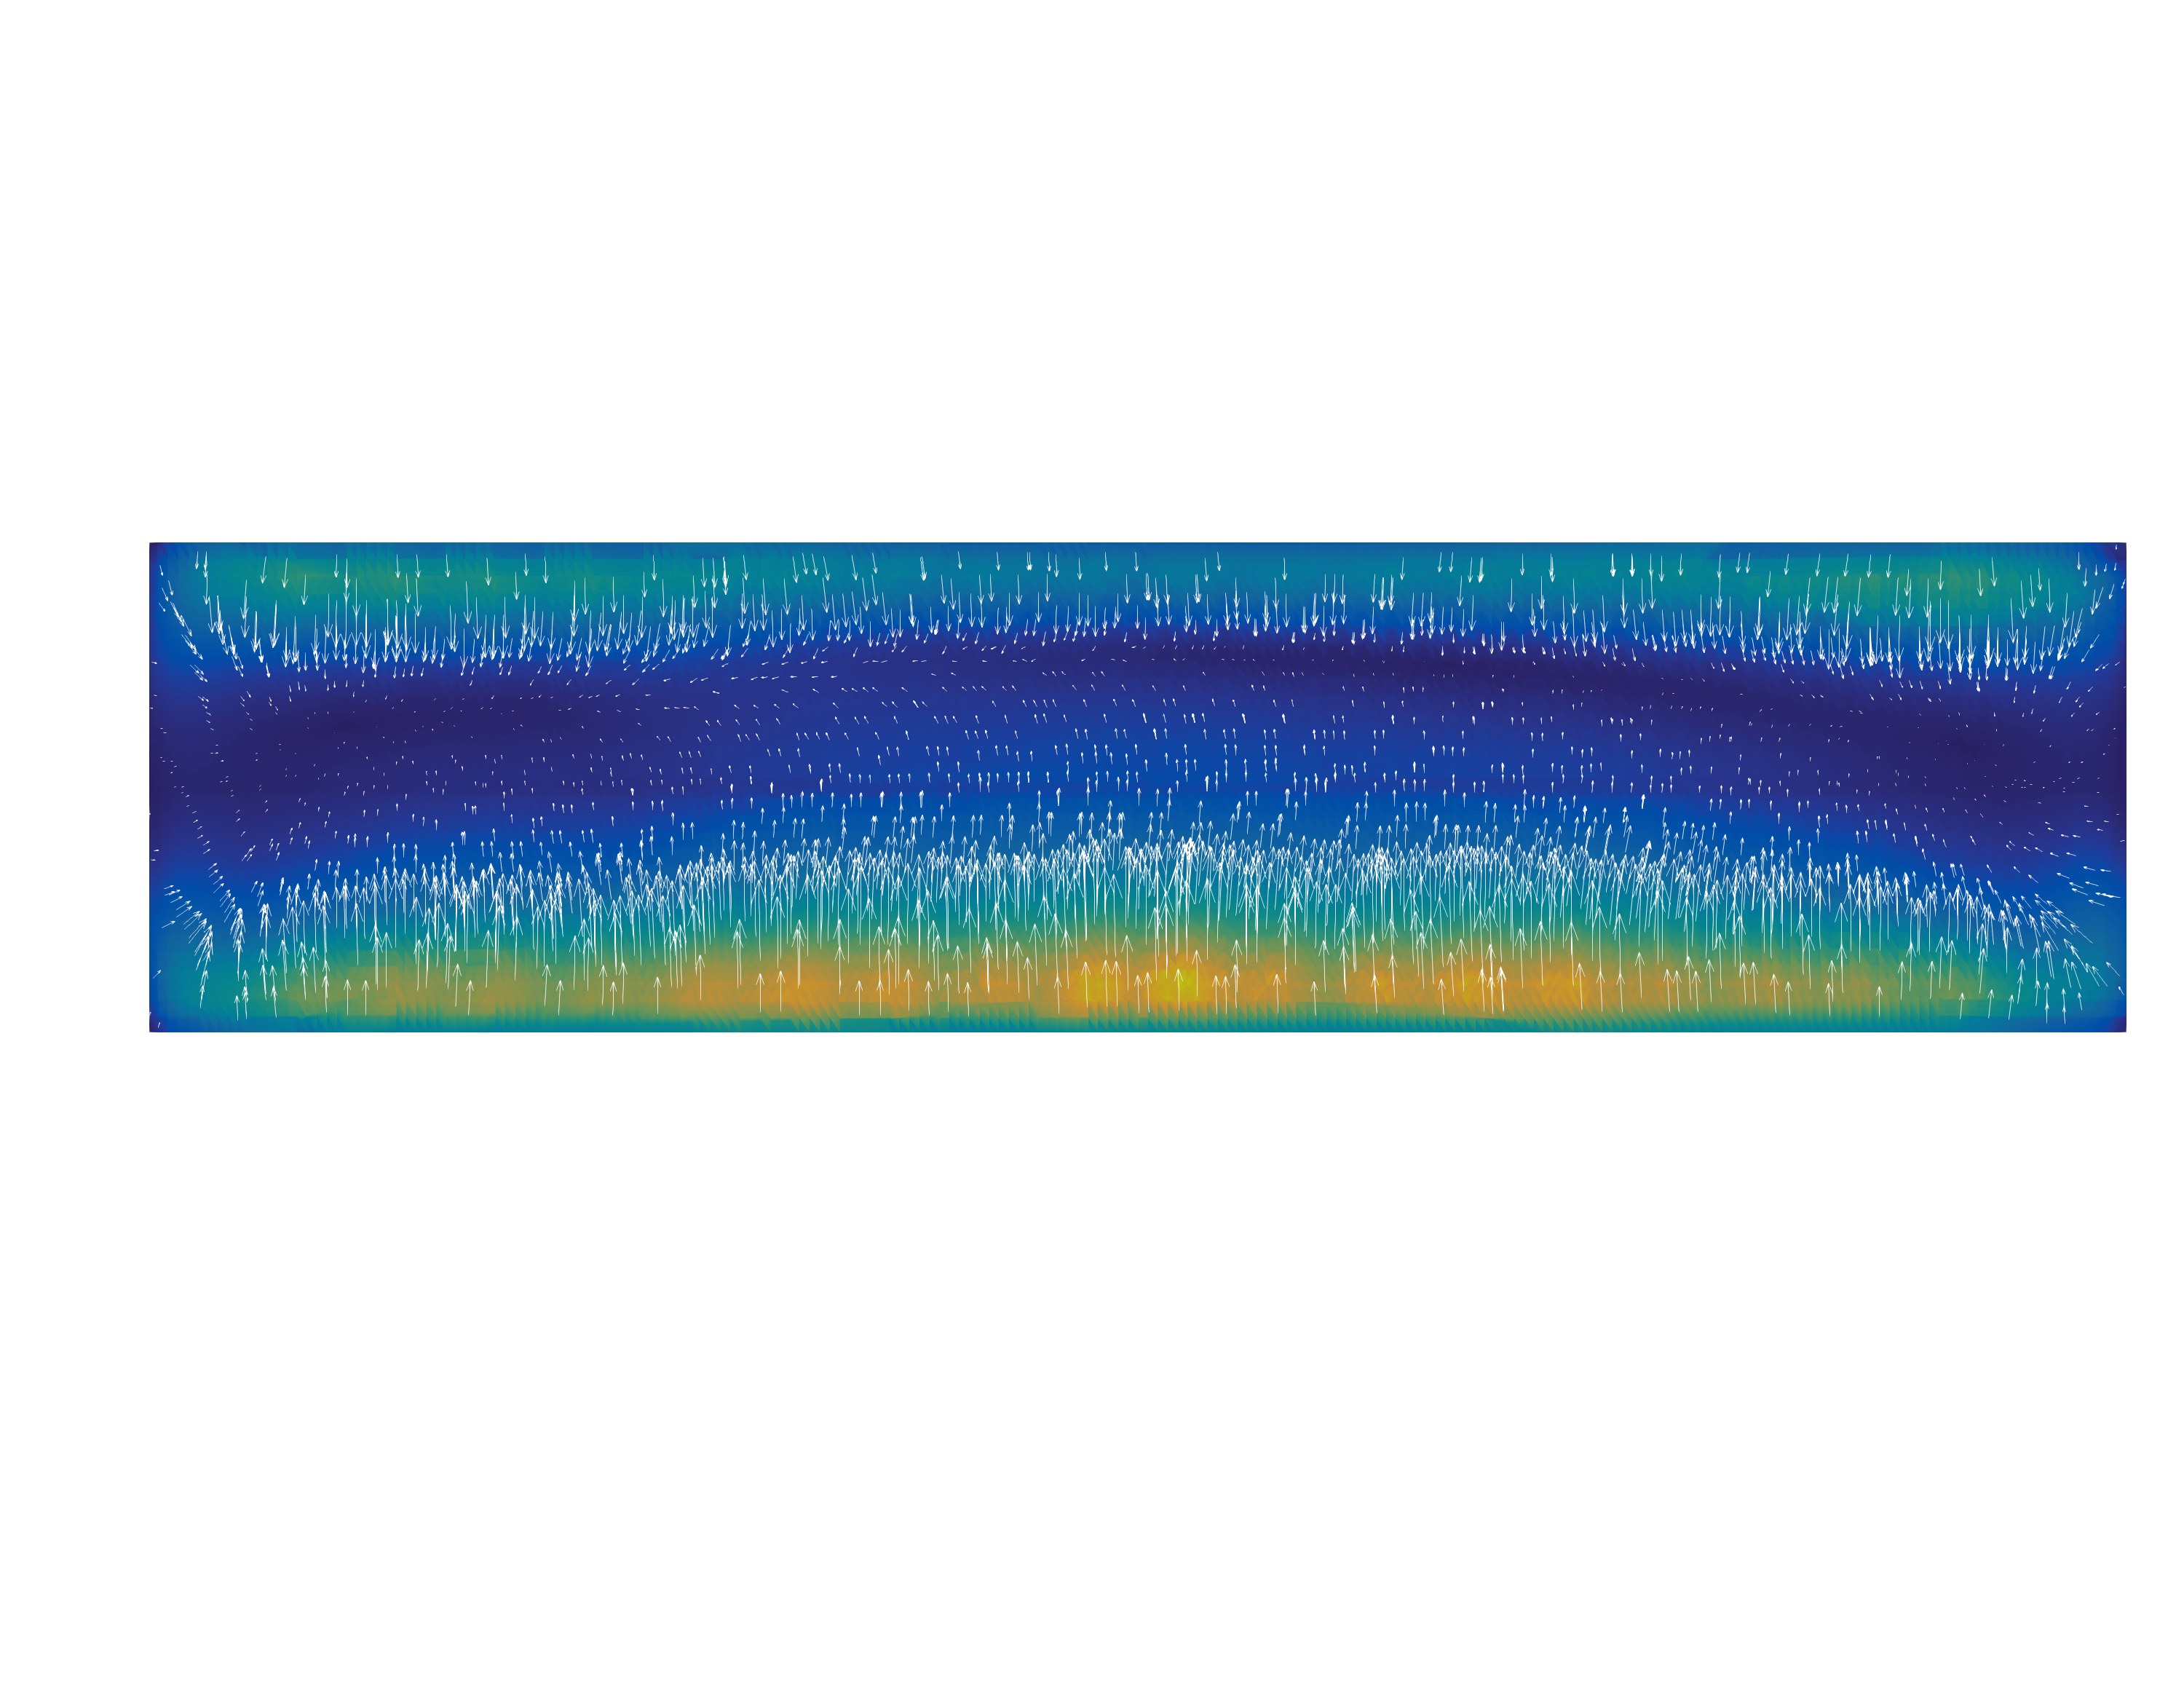
\includegraphics[width=\rasterimagewidth]{../media/fourier/application/print/force-h.png}};
      \end{axis}
    \end{tikzpicture}
    \caption{Champ de force $f$ dans le fluide issus du modèle 3D standard.}
    \label{fig:harmonic-force-h}
  \end{center}
\end{figure}

\begin{figure}[h!]
  \begin{center}
    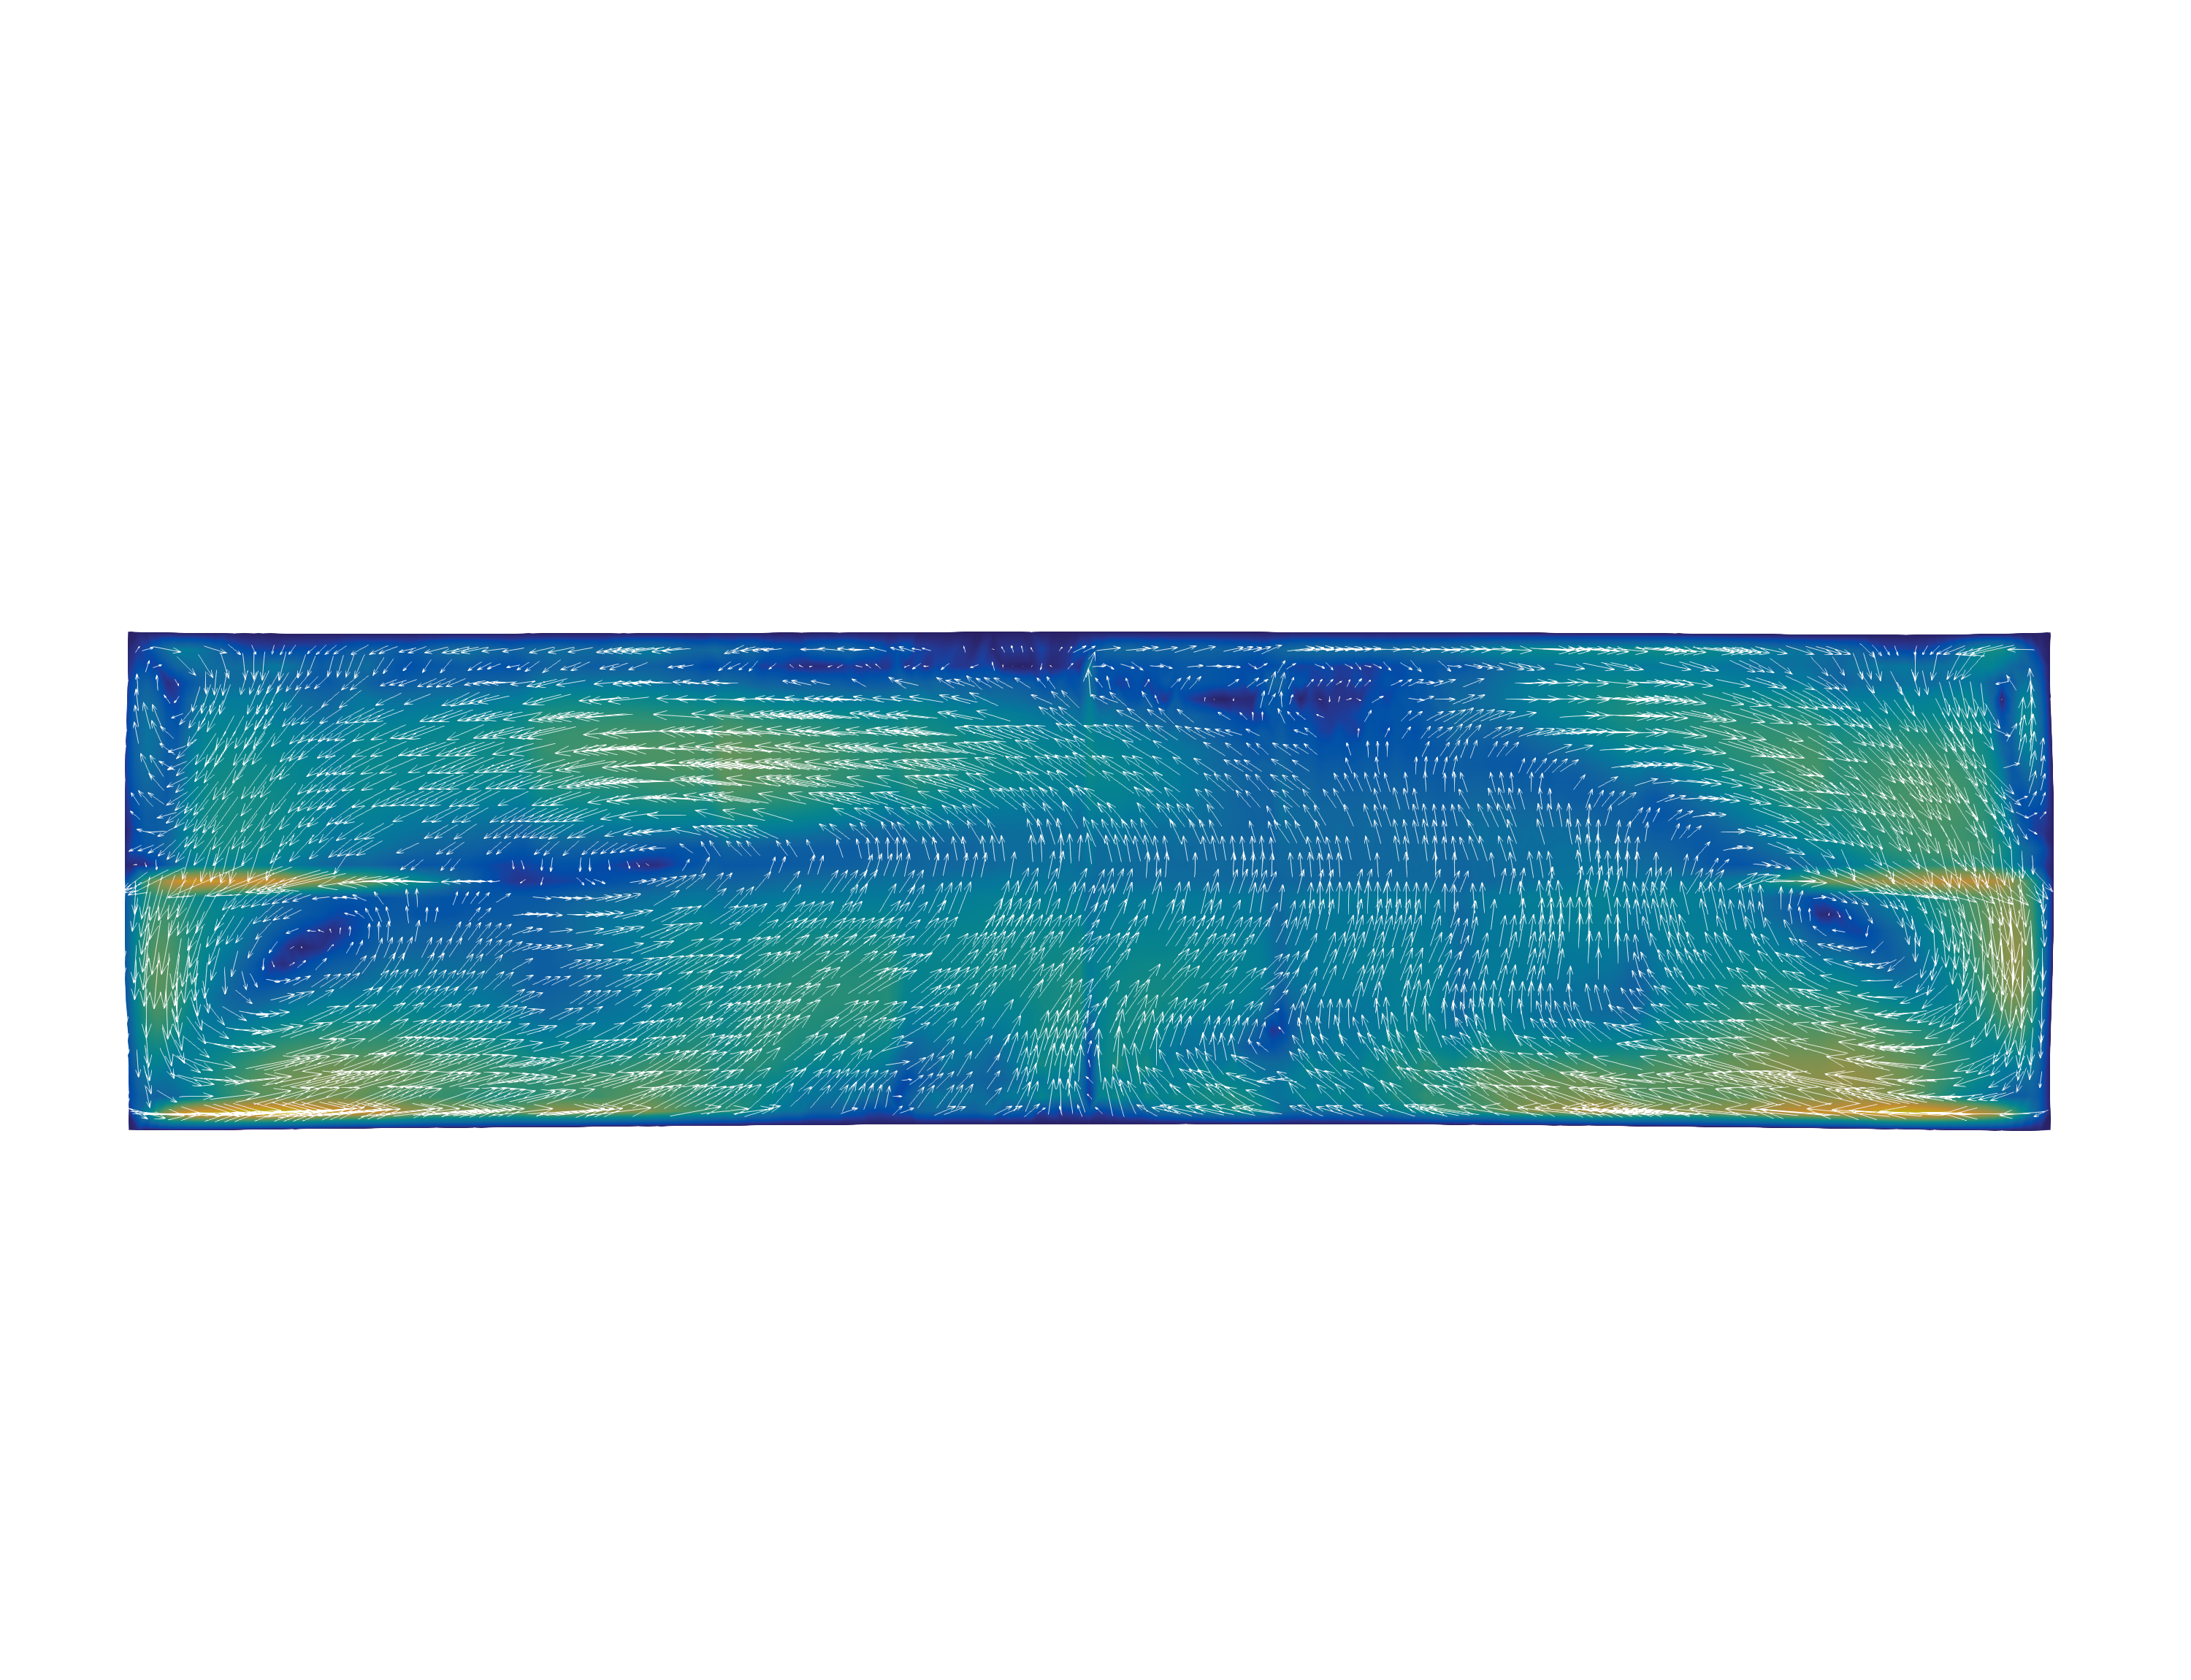
\includegraphics[width=\rasterimagewidth]{{../media/populations/ap32-fluid-flow/print/acd-all-anodes-velocity-0.00-0.05}.png}\\
    \begin{tikzpicture}
      \begin{axis}[
          colorbar,
          hide axis,
          scale only axis,
          height=0.41\rasterimagewidth,
          width=\rasterimagewidth,
          colorbar horizontal,
          point meta min=0.0,
          point meta max=6.0,
          colorbar style={
            title=Vitesse $u$ [\si{\centi\meter\per\second}],
            width=7.4cm,
            height=0.3cm,
            xtick={0.0, 3.0, 6.0},
            at={(0.5\rasterimagewidth,0.4cm)},
            anchor=north
          }
        ]
        \addplot [] coordinates {(0,0)};
        \node (myfirstpic) at (0,0) {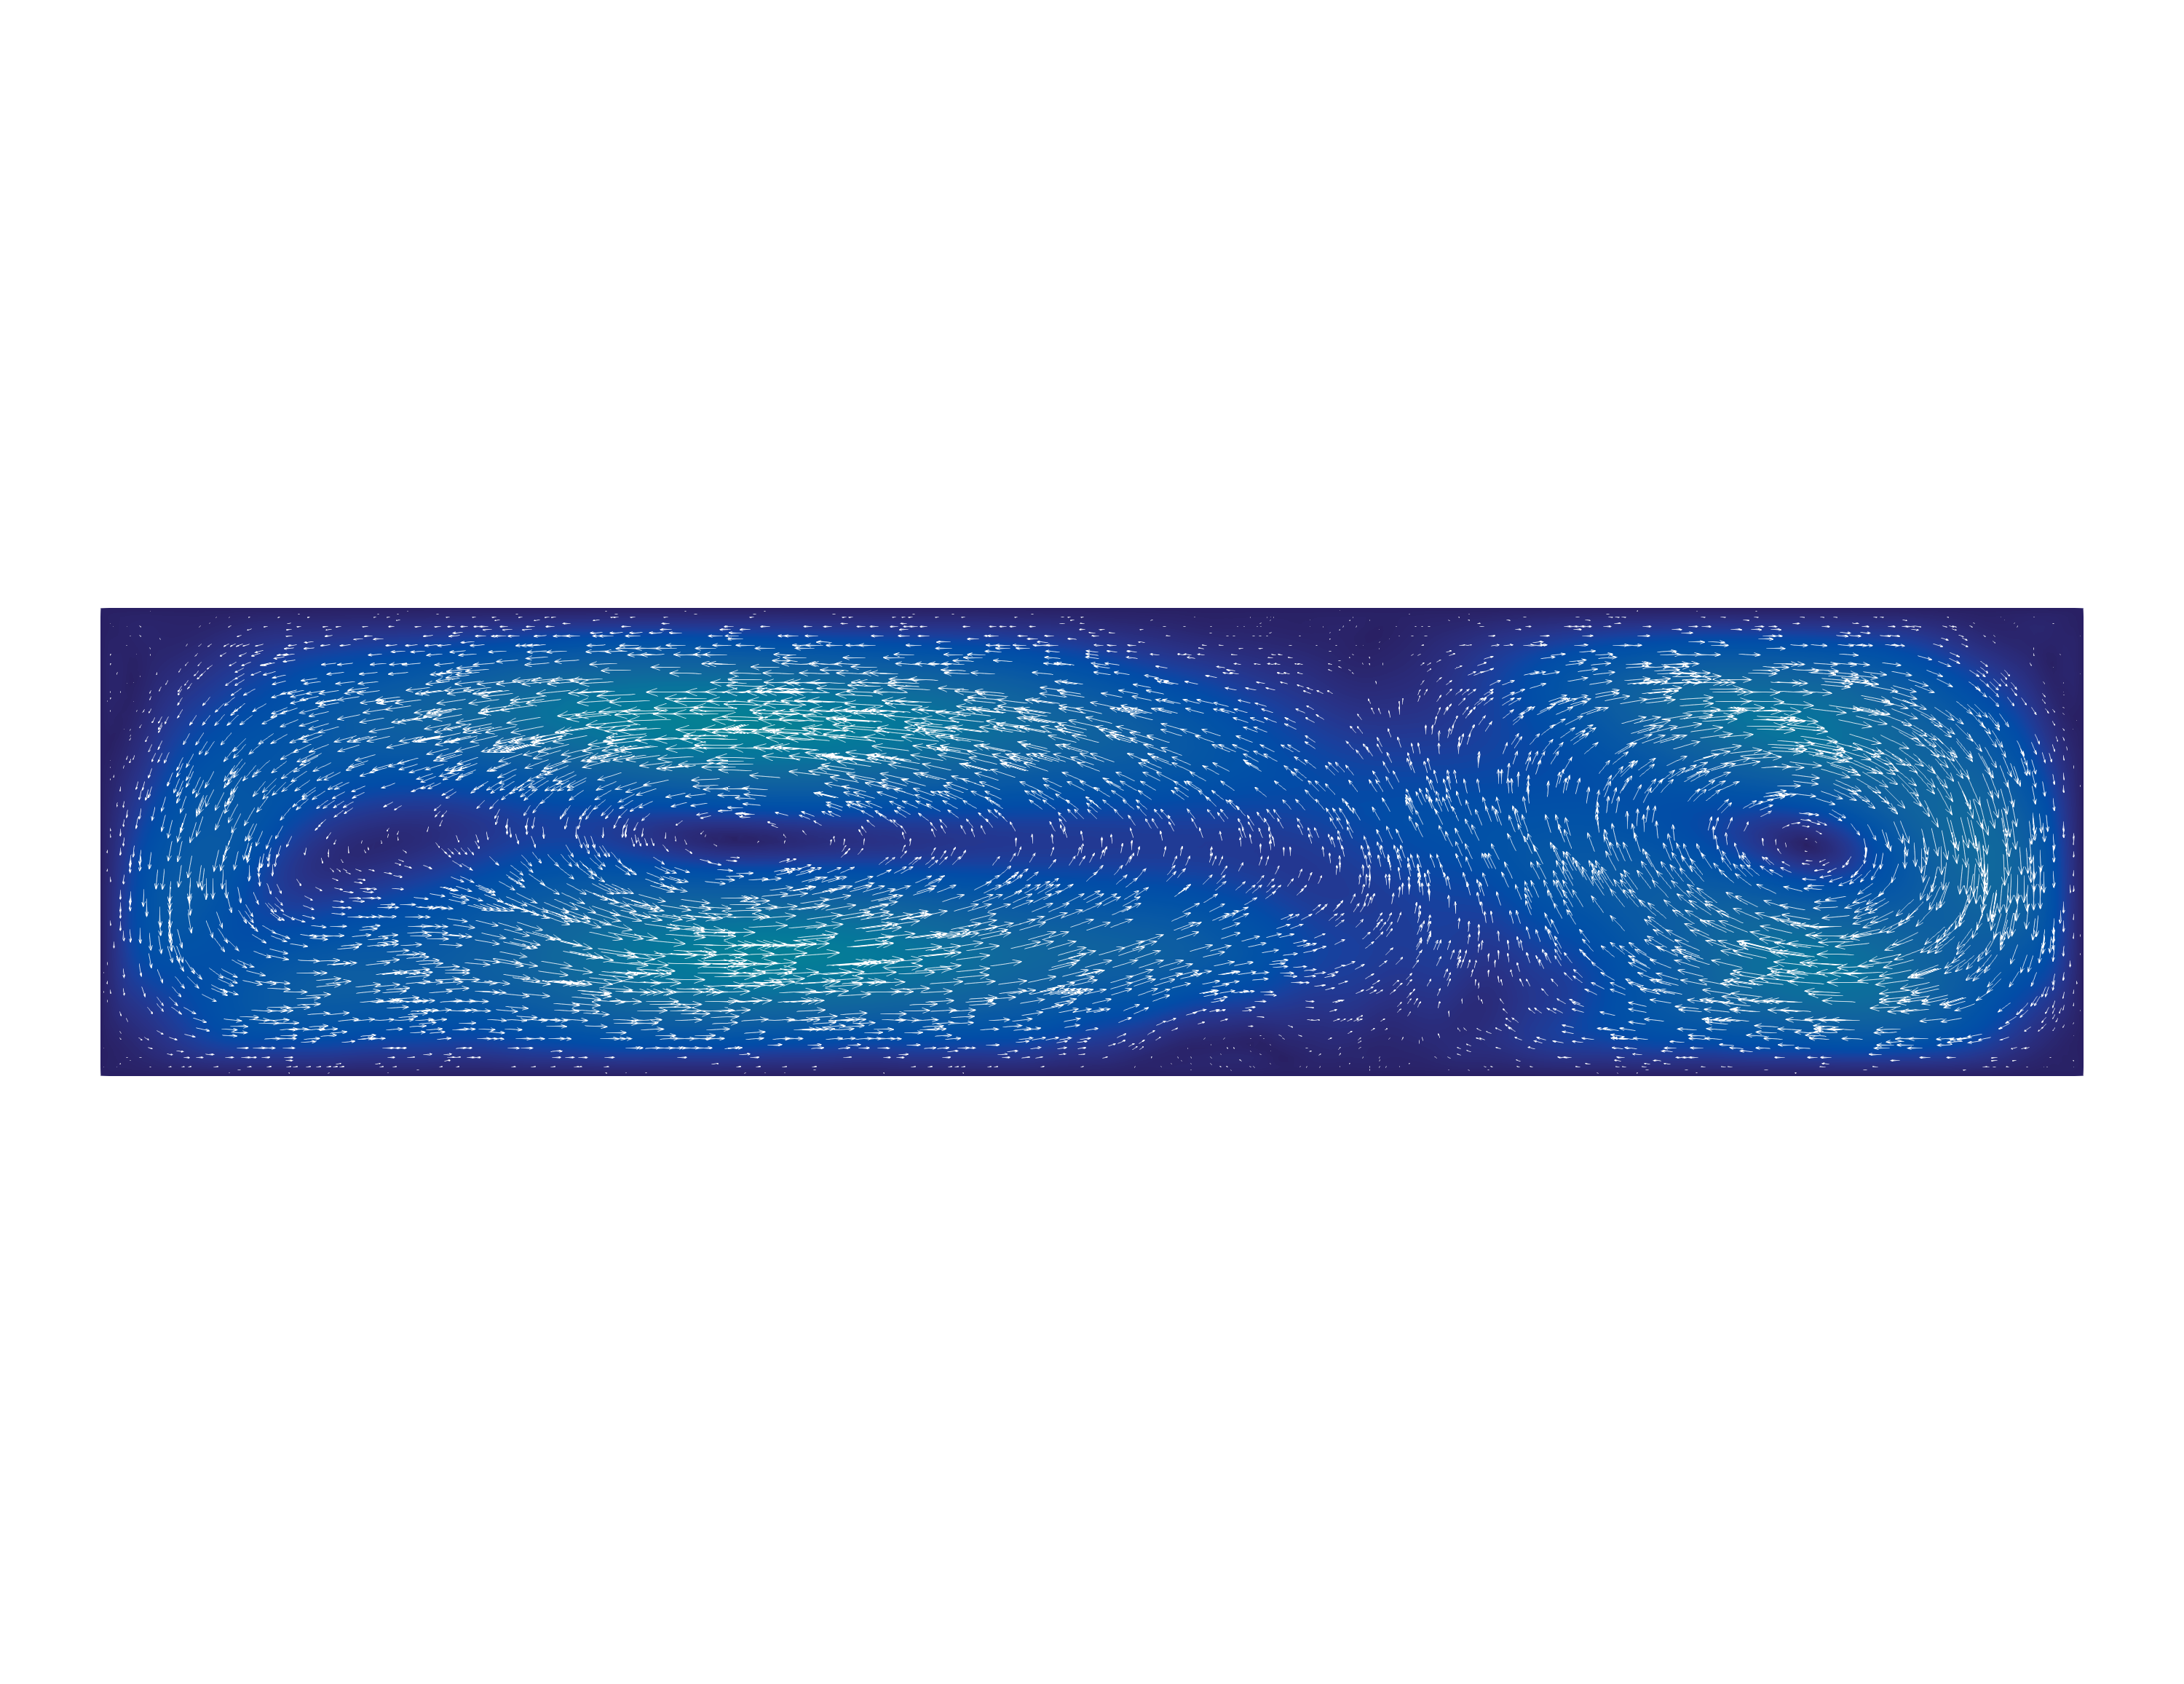
\includegraphics[width=\rasterimagewidth]{../media/fourier/application/print/all-velocity-harm.png}};
      \end{axis}
    \end{tikzpicture}
    \caption{Champ de vitesse stationnaire $u_h^{S3D}$ (haut) et
      $u_{h,K}^\mathrm{SF}$ reconstruit selon les équations
      (\ref{eq:u-h-12}), (\ref{eq:u-h-3}) (bas).}
    \label{fig:harmonic-velocity}
  \end{center}
\end{figure}

% conclusion:
%figure 4.6: \ref{fig:harmonic-velocity}
%figure 4.7: \ref{fig:harmonic-concentration}

On constate sur la figure \ref{fig:harmonic-velocity} que le champ de
courant $u_{h,K}^{\mathrm{SF}}$ reproduit les grandes structures de
l'écoulement $u_h^{\mathrm{S3D}}$: deux tourbillons principaux divise
la cuve, et la position de leur frontière correspond. Cependant, le
champ $u_{h,K}^{\mathrm{SF}}$ ne parvient pas a capturer les plus
petites structures qui apparaissent dans $u_h^{\mathrm{S3D}}$, soient
les petits tourbillons secondaires dans les coins en aval, ainsi
qu'une certaine asymétrie général par rapport à l'axe $x$.

\begin{figure}[h!]
  \begin{center}
    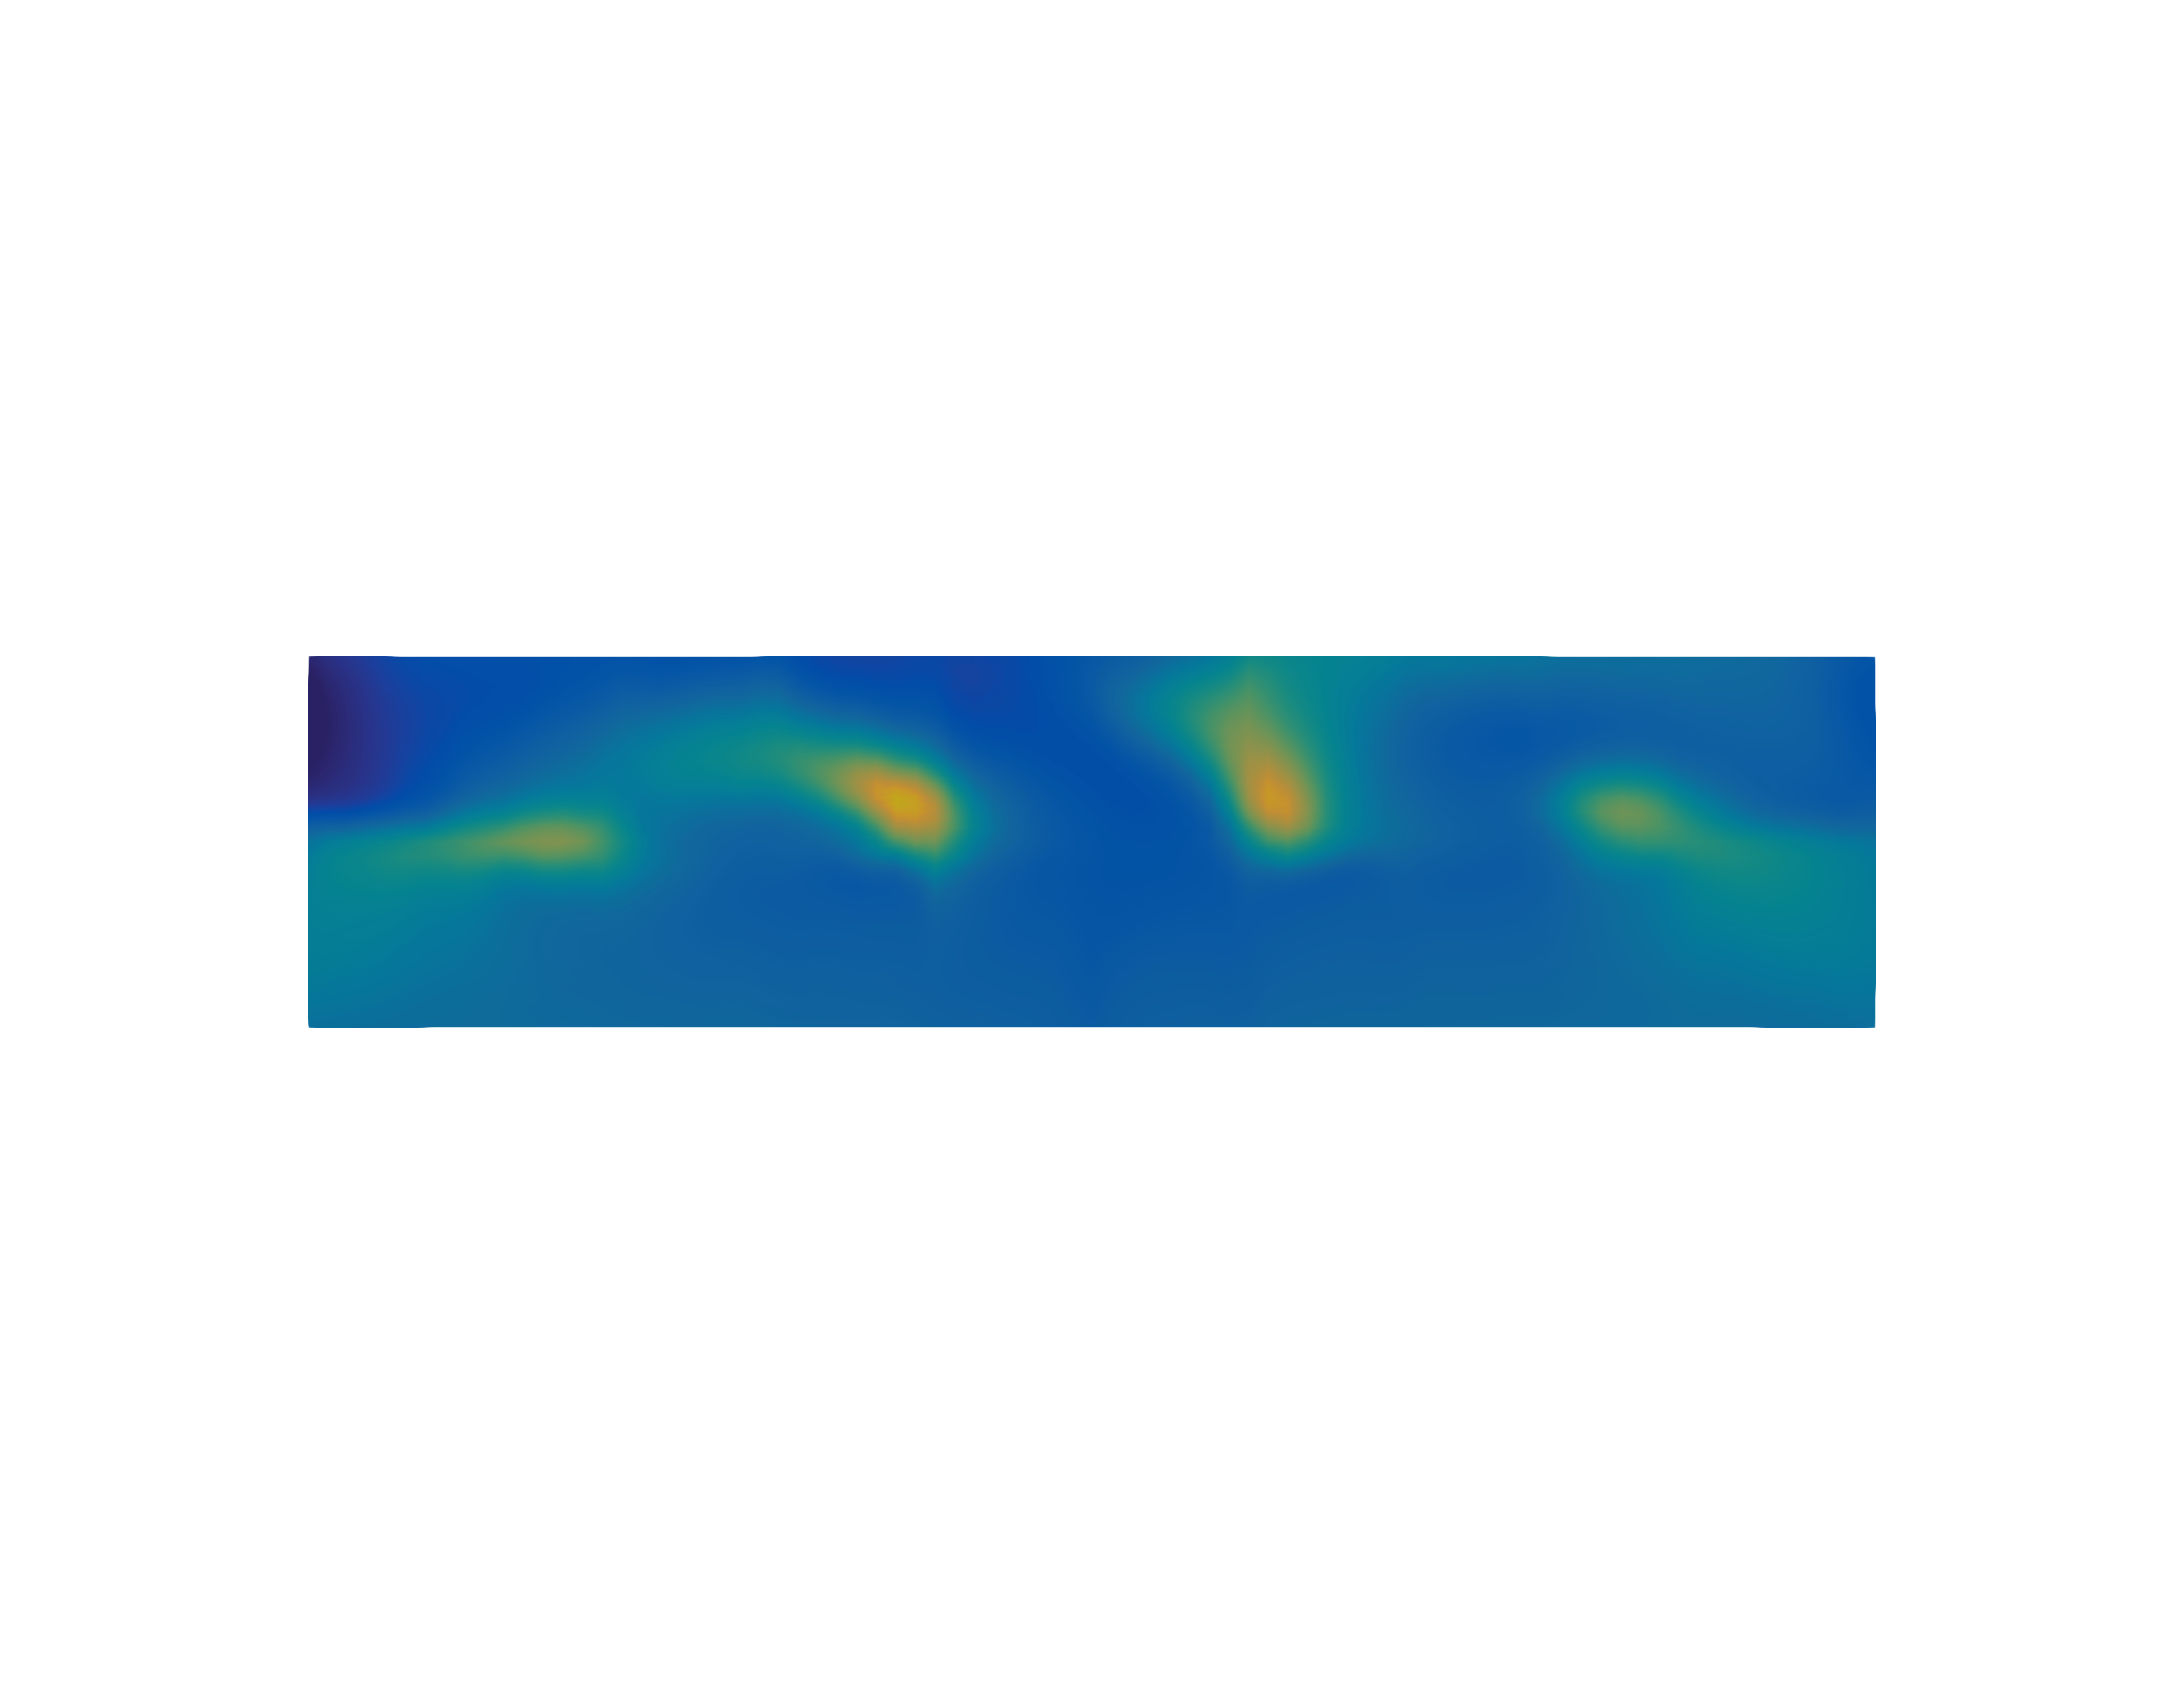
\includegraphics[width=\rasterimagewidth]{{../media/fourier/application/print/all-concentration-acd}.png}\\
    \begin{tikzpicture}
      \begin{axis}[
          colorbar,
          hide axis,
          scale only axis,
          height=0.41\rasterimagewidth,
          width=\rasterimagewidth,
          colorbar horizontal,
          point meta min=1.73,
          point meta max=6.84,
          colorbar style={
            title=Concentration $c$ [w\%],
            width=7.4cm,
            height=0.3cm,
            xtick={1.73, 3.0, 5.0, 6.84},
            at={(0.5\rasterimagewidth,0.4cm)},
            anchor=north
          }
        ]
        \addplot [] coordinates {(0,0)};
        \node (myfirstpic) at (0,0) {
          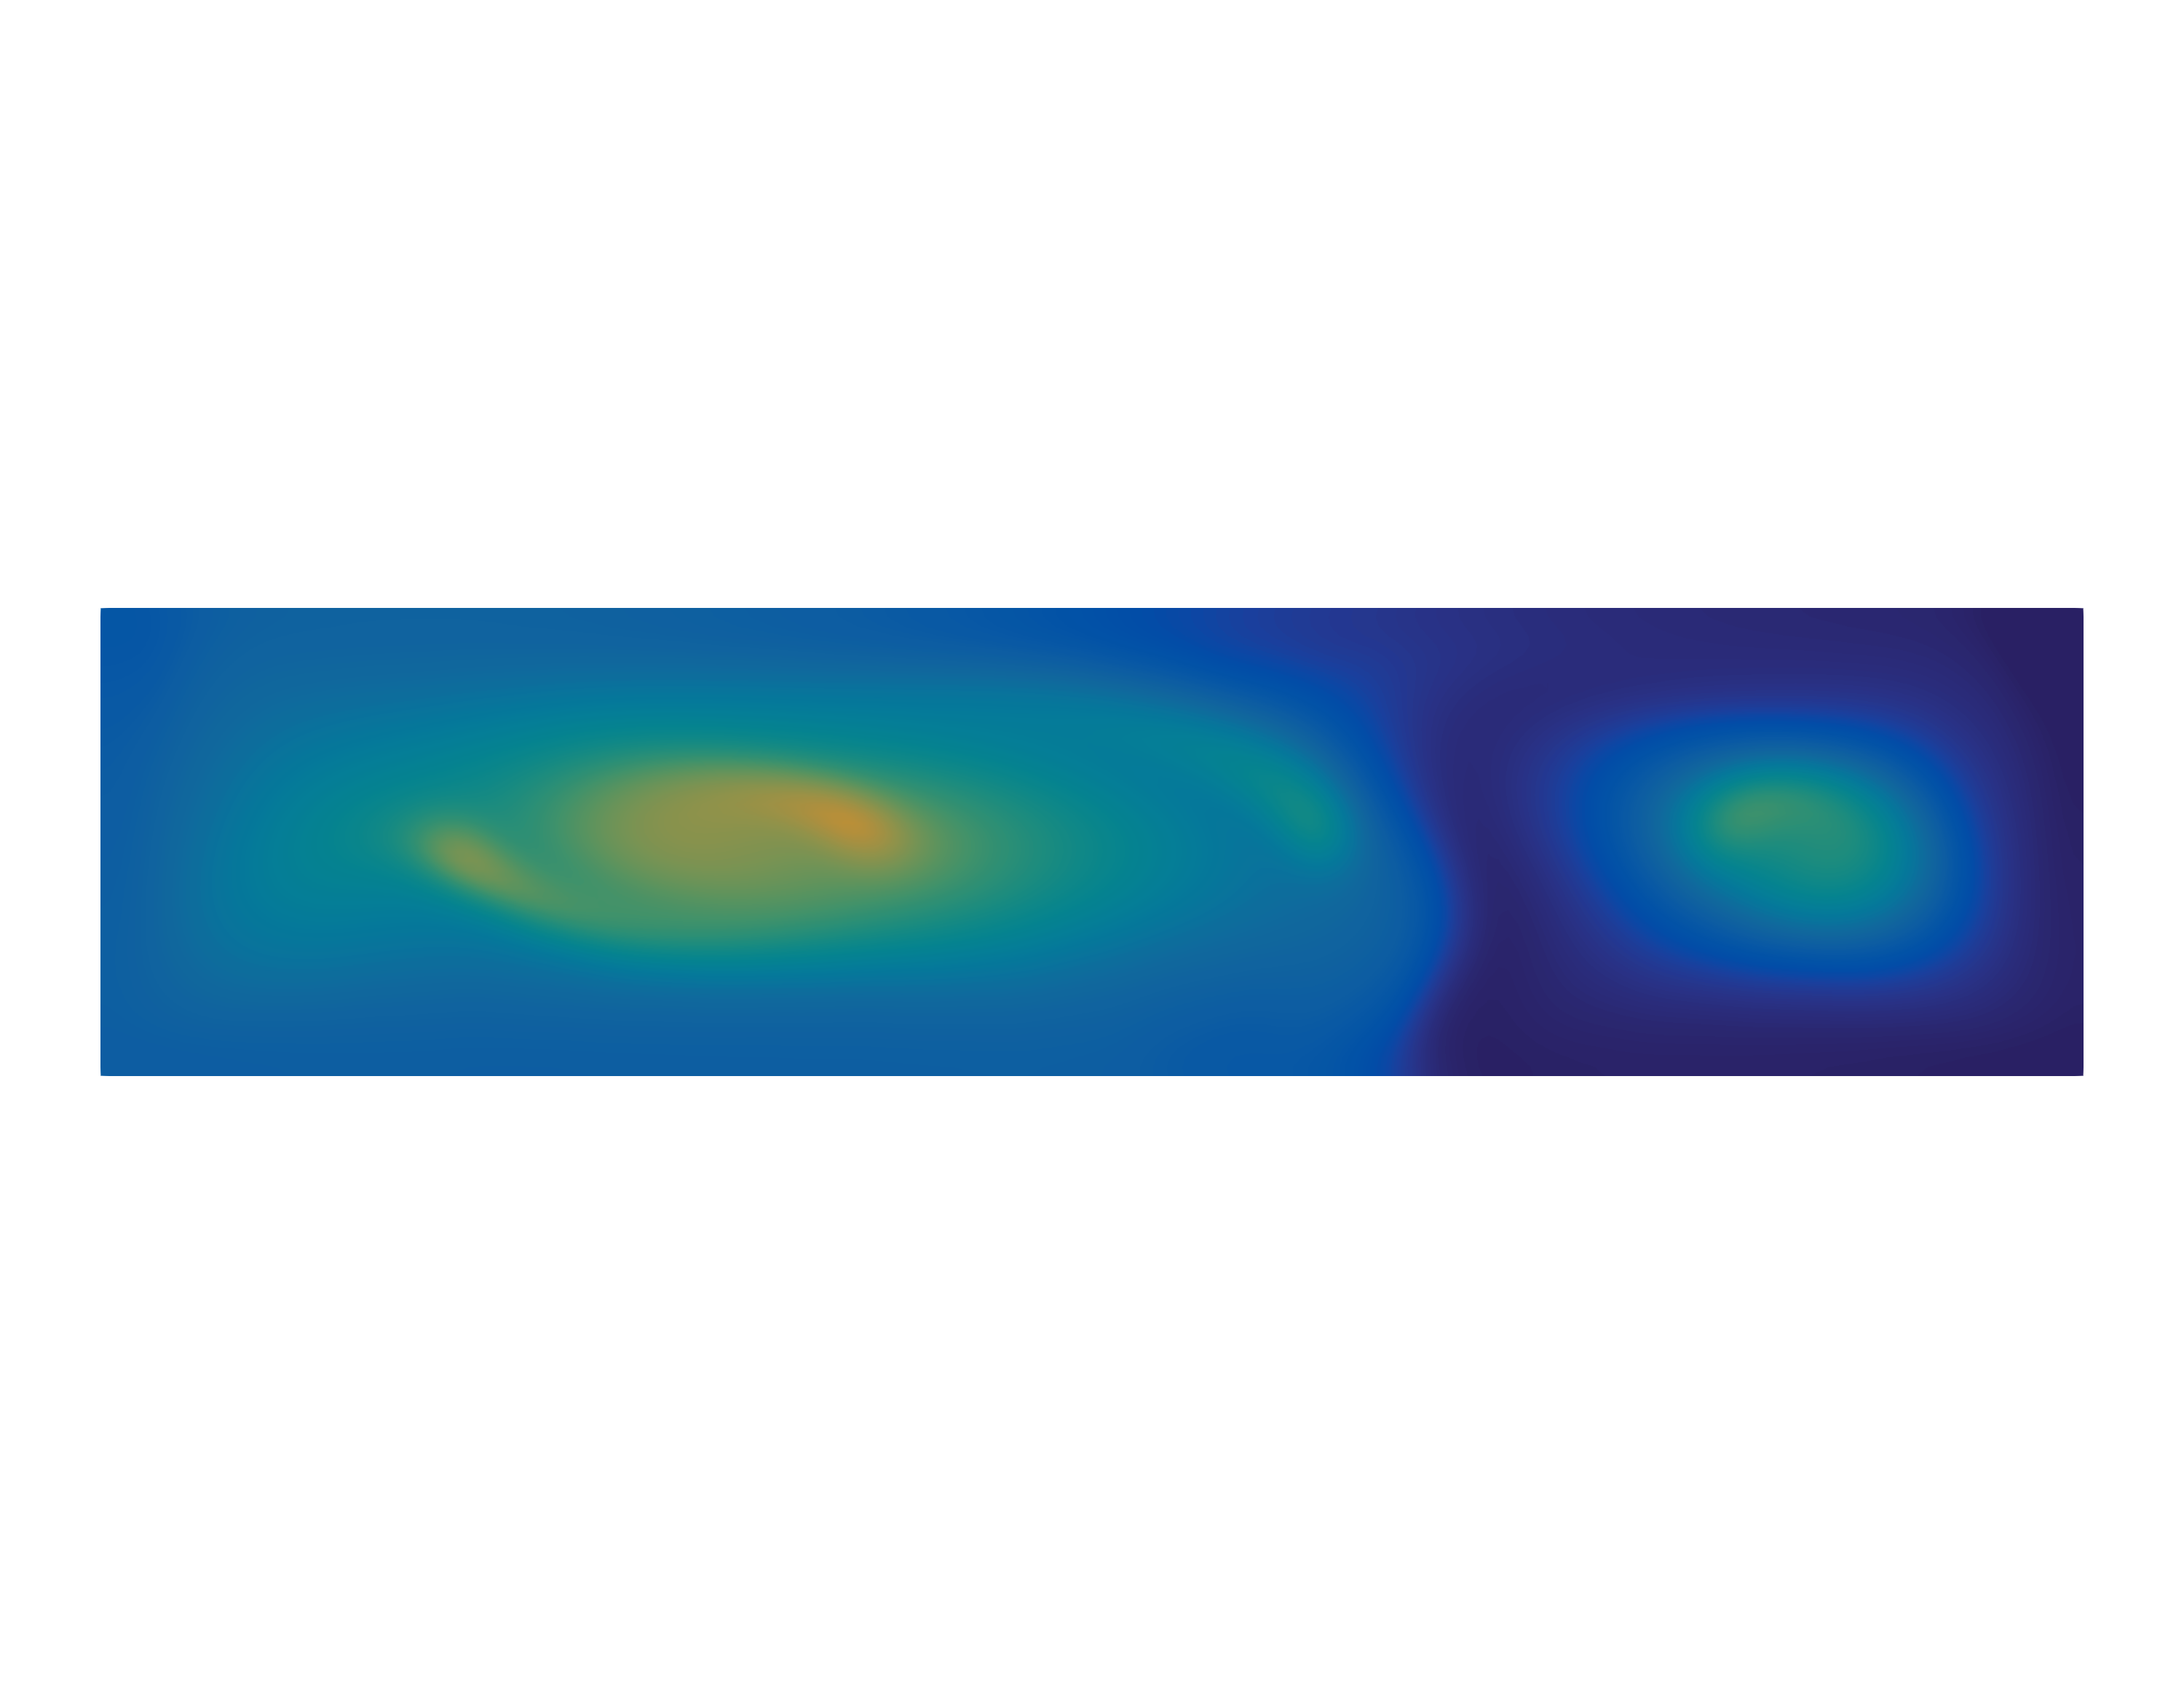
\includegraphics
              [width=\rasterimagewidth]
              {../media/fourier/application/print/all-concentration-harm.png}
        };
      \end{axis}
    \end{tikzpicture}
    \caption{Champ de concentration stationnaire $c_h^\mathrm{S3D}$
      (haut) et $c_{h}^\mathrm{SF}$
      solution de l'équation (\ref{eq:stat-concentration}) (bas).}
    \label{fig:harmonic-concentration}
  \end{center}
\end{figure}

En comparaison avec le champ $c_h^\mathrm{S3D}$ (en
haut sur la figure \ref{fig:harmonic-concentration}), le champ de
concentration stationnaire $c_h^\mathrm{SF}$ (en bas sur la
figure \ref{fig:harmonic-concentration}) reproduit certains aspects
caractéristiques. En particulier, les amplitudes de variation de la
concentration sont très similaires. De plus, la position des points
d'injections apparaît clairement dans sur les deux calculs. En
revanche, le champ $c_h^\mathrm{SF}$ présente une zone appauvrie en
périphérie du tourbillon de droite, qui n'est pas présente dans
le champ $c_h^\mathrm{S3D}$.

\subsection{Désactivation d'anodes}
On s'intéresse maintenant au cas du calcul de l'écoulement des fluides
et de la concentration d'alumine dissoute dans le bain électrolytique
lorsqu'on désactive une anode, c'est-à-dire que l'une des anodes du
plan anodique n'est pas conductrice électriquement. Cette situation a
lieu en pratique lorsqu'une anode en fin de vie est remplacée par une
anode neuve, mais froide. Sa conductivité électrique qui est
quasi-nulle initialement, augmente au fur et à mesure que l'anode
atteint sa température d'opération. Dans cette partie, on dénotera
conjointement la vitesse du fluide stationnaire et la concentration
d'alumine dissoute obtenue qui résultent du modèle décrit dans le
chapitre \ref{chap:populations} par l'abréviation S3D. Dans cette
partie, on considérera uniquement une dissolution des particules
d'alumine indépendante de la température, c'est-à-dire que le champ
$c^\mathrm{S3D}$ est calculé avec le modèle standard 3D (S3D) en désactivant
la dépendance de la vitesse de dissolution en fonction de la
température du bain.

Dans le modèle S3D, on peut simuler la désactivation d'une anode en
annulant la conductivité électrique $\conductivity$ dans le volume
occupé par ladite anode. On a donc la densité de courant $j =
\conductivity\parent{\nabla \phi + u^\mathrm{S3D}}$, $\div j = 0$, où
$\phi$ est le potentiel électrique, $u^\mathrm{S3D}$ l'écoulement des
fluides solution des équations de Navier-Stokes, $B$ le champ
d'induction magnétique solution des équations de Maxwell et la force
$f = j\times B$. Dans le modèle SF, on utilise le champ de force $f$
issus d'un calcul S3D avec toutes les anodes activées, restreint à
$\Omega$. On simule la désactivation d'une anode en supposant que la
densité de courant électrique est quasiment nulle sous celle-ci, ce
qui revient à imposer $f = 0$ sous l'anode désactivée (voir figure
\ref{fig:anode-deactivation}). L'emplacement des anodes vues depuis
dessus et leur numérotation dans la cuve AP32 est schématisé sur la
figure \ref{fig:anode-numerotations}.

Les figures \ref{fig:f3d-deactivated-a}, \ref{fig:f3d-deactivated-b},
présente le champ de vitesse stationnaire $u^{S3D}$ du bain
électrolytique dans l'ACD de la cuve AP32 et la distribution de
concentration $c^{S3D}$, pour quatre configurations différentes du
plan anodique, soit les anodes $(1,1)$, $(1,2)$, $(2,1)$ et $(2,2)$
successivement désactivées. On se réfère à la figure
\ref{fig:anode-numerotations} pour le placement de chacune de ces
anodes. Les anodes désactivées se trouvent au niveau de l'extrémité
gauche de la cuve. On note que l'influence sur le champ de vitesse et
la distribution de concentration s'étend à proximité de l'anode
désactivée, mais ne s'étend pas à l'ensemble de la cuve.

\begin{figure}[h!]
  \begin{center}
    \input{../media/fourier/anode-deactivation/anode-deactivation.pdf_tex}
    \caption{Désactivation d'une anode dans le modèle standard S3D et
      le modèle SF. (a) Dans le modèle S3D, la désactivation d'une
      anode est modélisée par l'annulation de sa conductivité
      électrique $\conductivity$. (b.1) Calcul du terme de force avec
      le modèle S3D et toutes les anodes activées. (b.2) Calcul de
      l'écoulement dans le domaine $\Omega$ avec le modèle SF et la
      force obtenue en (b.1), mais annulée sous l'anode désactivée.}
    \label{fig:anode-deactivation}
  \end{center}
\end{figure}


% figures 4.12, 4.13
Pour évaluer l'effet des approximations introduites par le modèle
SF par rapport au modèle S3D, on compare les champs de vitesse
$u_h^{\mathrm{S3D}}$ et $u_h^{\mathrm{SF}}$. Pour le calcul de
$u_h^{\mathrm{SF}}$, on utilise le champ de force $f$ issus du calcul de
$u_h^{\mathrm{S3D}}$. Sur les figures \ref{fig:harmonic-velocity-comp-a}, \ref{fig:harmonic-velocity-comp-b}
on peut comparer les champs de vitesse $u_h^{\mathrm{S3D}}$ et
$u_h^\mathrm{SF}$ sur une surface horizontale placée respectivement
dans l'ACD de la cuve AP32 ou dans le domaine $\Omega$ à une hauteur
correspondante.


%figure 4.14, 4.15
L'objectif final est de calculer le champ de concentration d'alumine
dans le bain électrolytique. Sur les figures
\ref{fig:harmonic-concentration-comp-a},
\ref{fig:harmonic-concentration-comp-b}, on compare les champs de
concentration $c^\mathrm{S3D}$ et le champ de concentration
stationnaire $c^\mathrm{SF}$ dans le domaine $\Omega$ avec le modèle
SF. On obtient le champ de transport $u_h^\mathrm{SF}$ qui sert au
calcul de $c_h^\mathrm{SF}$ en utilisant le champ de force $f$ issus
du calcul de $u^\mathrm{S3D}$ avec l'anode correspondante désactivée
(voir figure \ref{fig:anode-deactivation}a).

\begin{figure}[h!]
  \begin{center}
    \input{../media/fourier/anode-numerotations/anode-numerotation.pdf_tex}
    \caption{Numérotation des anodes de la cuve AP32.}
    \label{fig:anode-numerotations}
  \end{center}
\end{figure}

L'objectif du modèle étant d'obtenir une approximation du champ de
vitesse et du champ de concentration à moindre coût, on veut éviter à
tout prix de devoir utiliser le modèle S3D pour obtenir le champ de
force en fonction de la configuration du plan anodique. A la place, on
effectue un calcul de la force que l'on note $f^0$ avec le modèle S3D
dans la configuration où toutes les anodes sont actives (voir figure
\ref{fig:anode-deactivation}b.1 et
\ref{fig:anode-deactivation}b.2). La force $f^0$ est représentée sur
la figure \ref{fig:harmonic-force-h}.

\begin{figure}[!h]
  \begin{center}
    \begin{subfigure}[t]{\textwidth}
      \begin{center}
        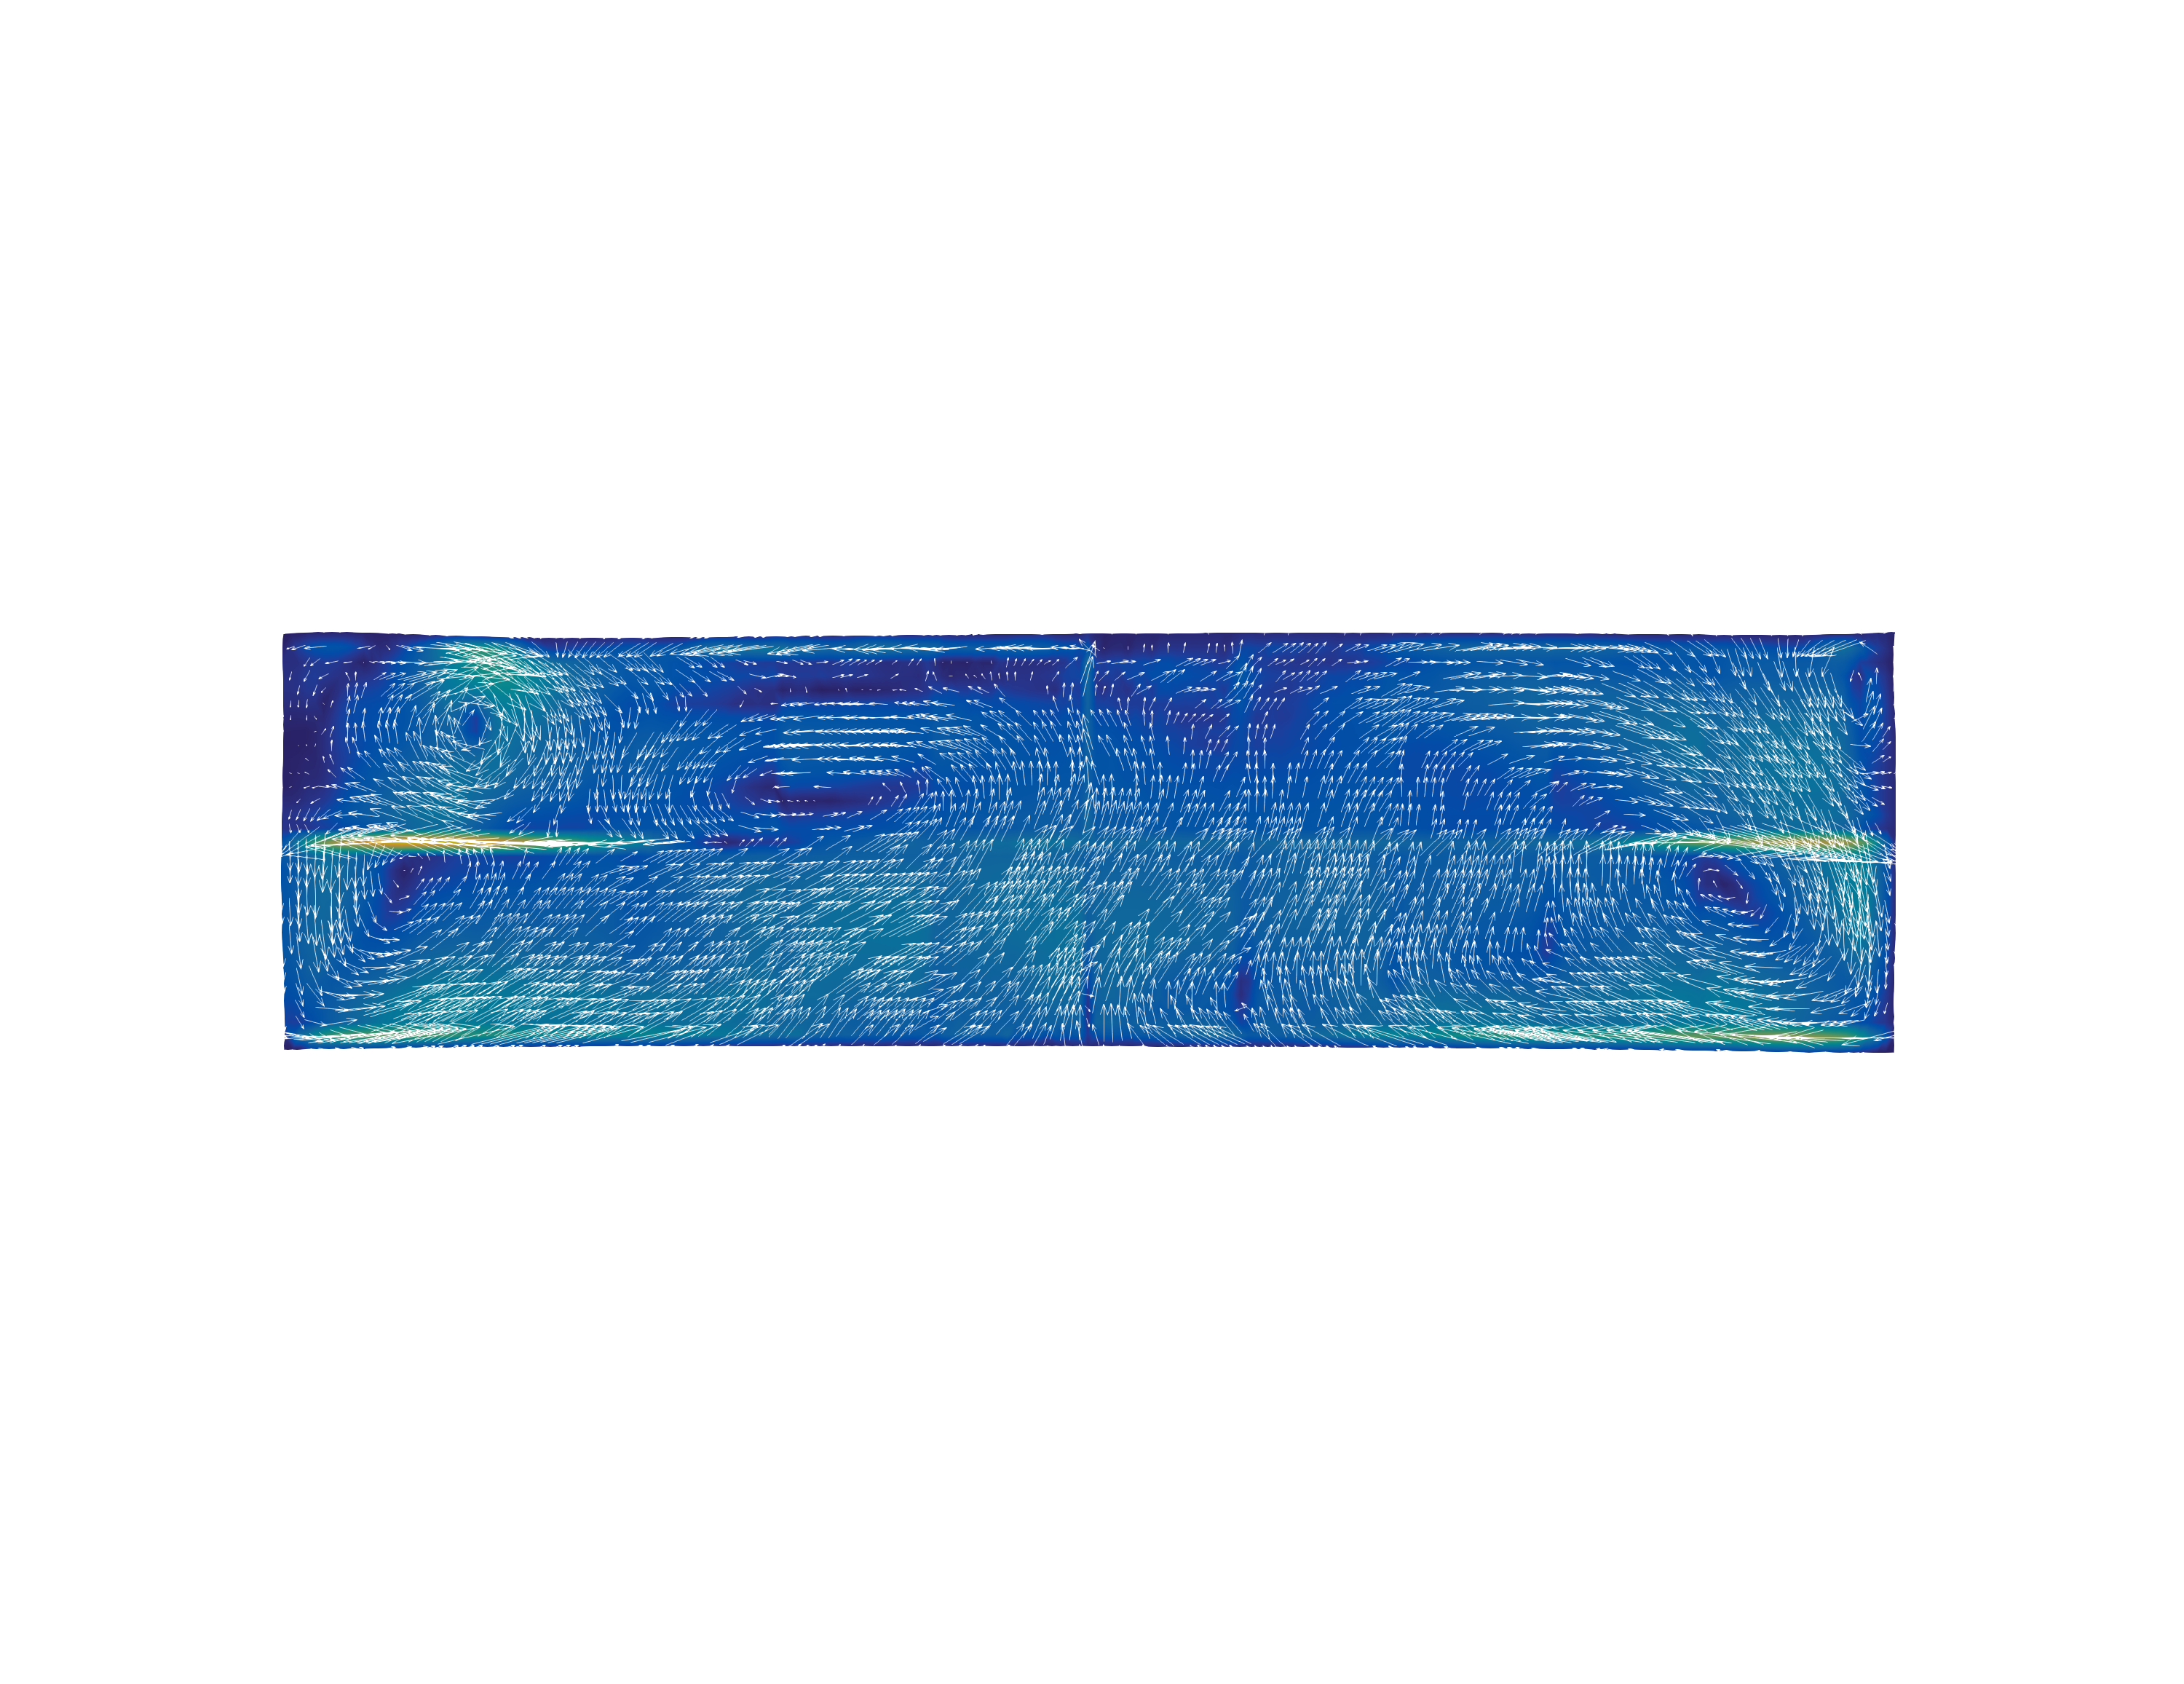
\includegraphics[width=0.9\textwidth]{../media/fourier/application/print/ab-0-1-velocity-acd.png}
        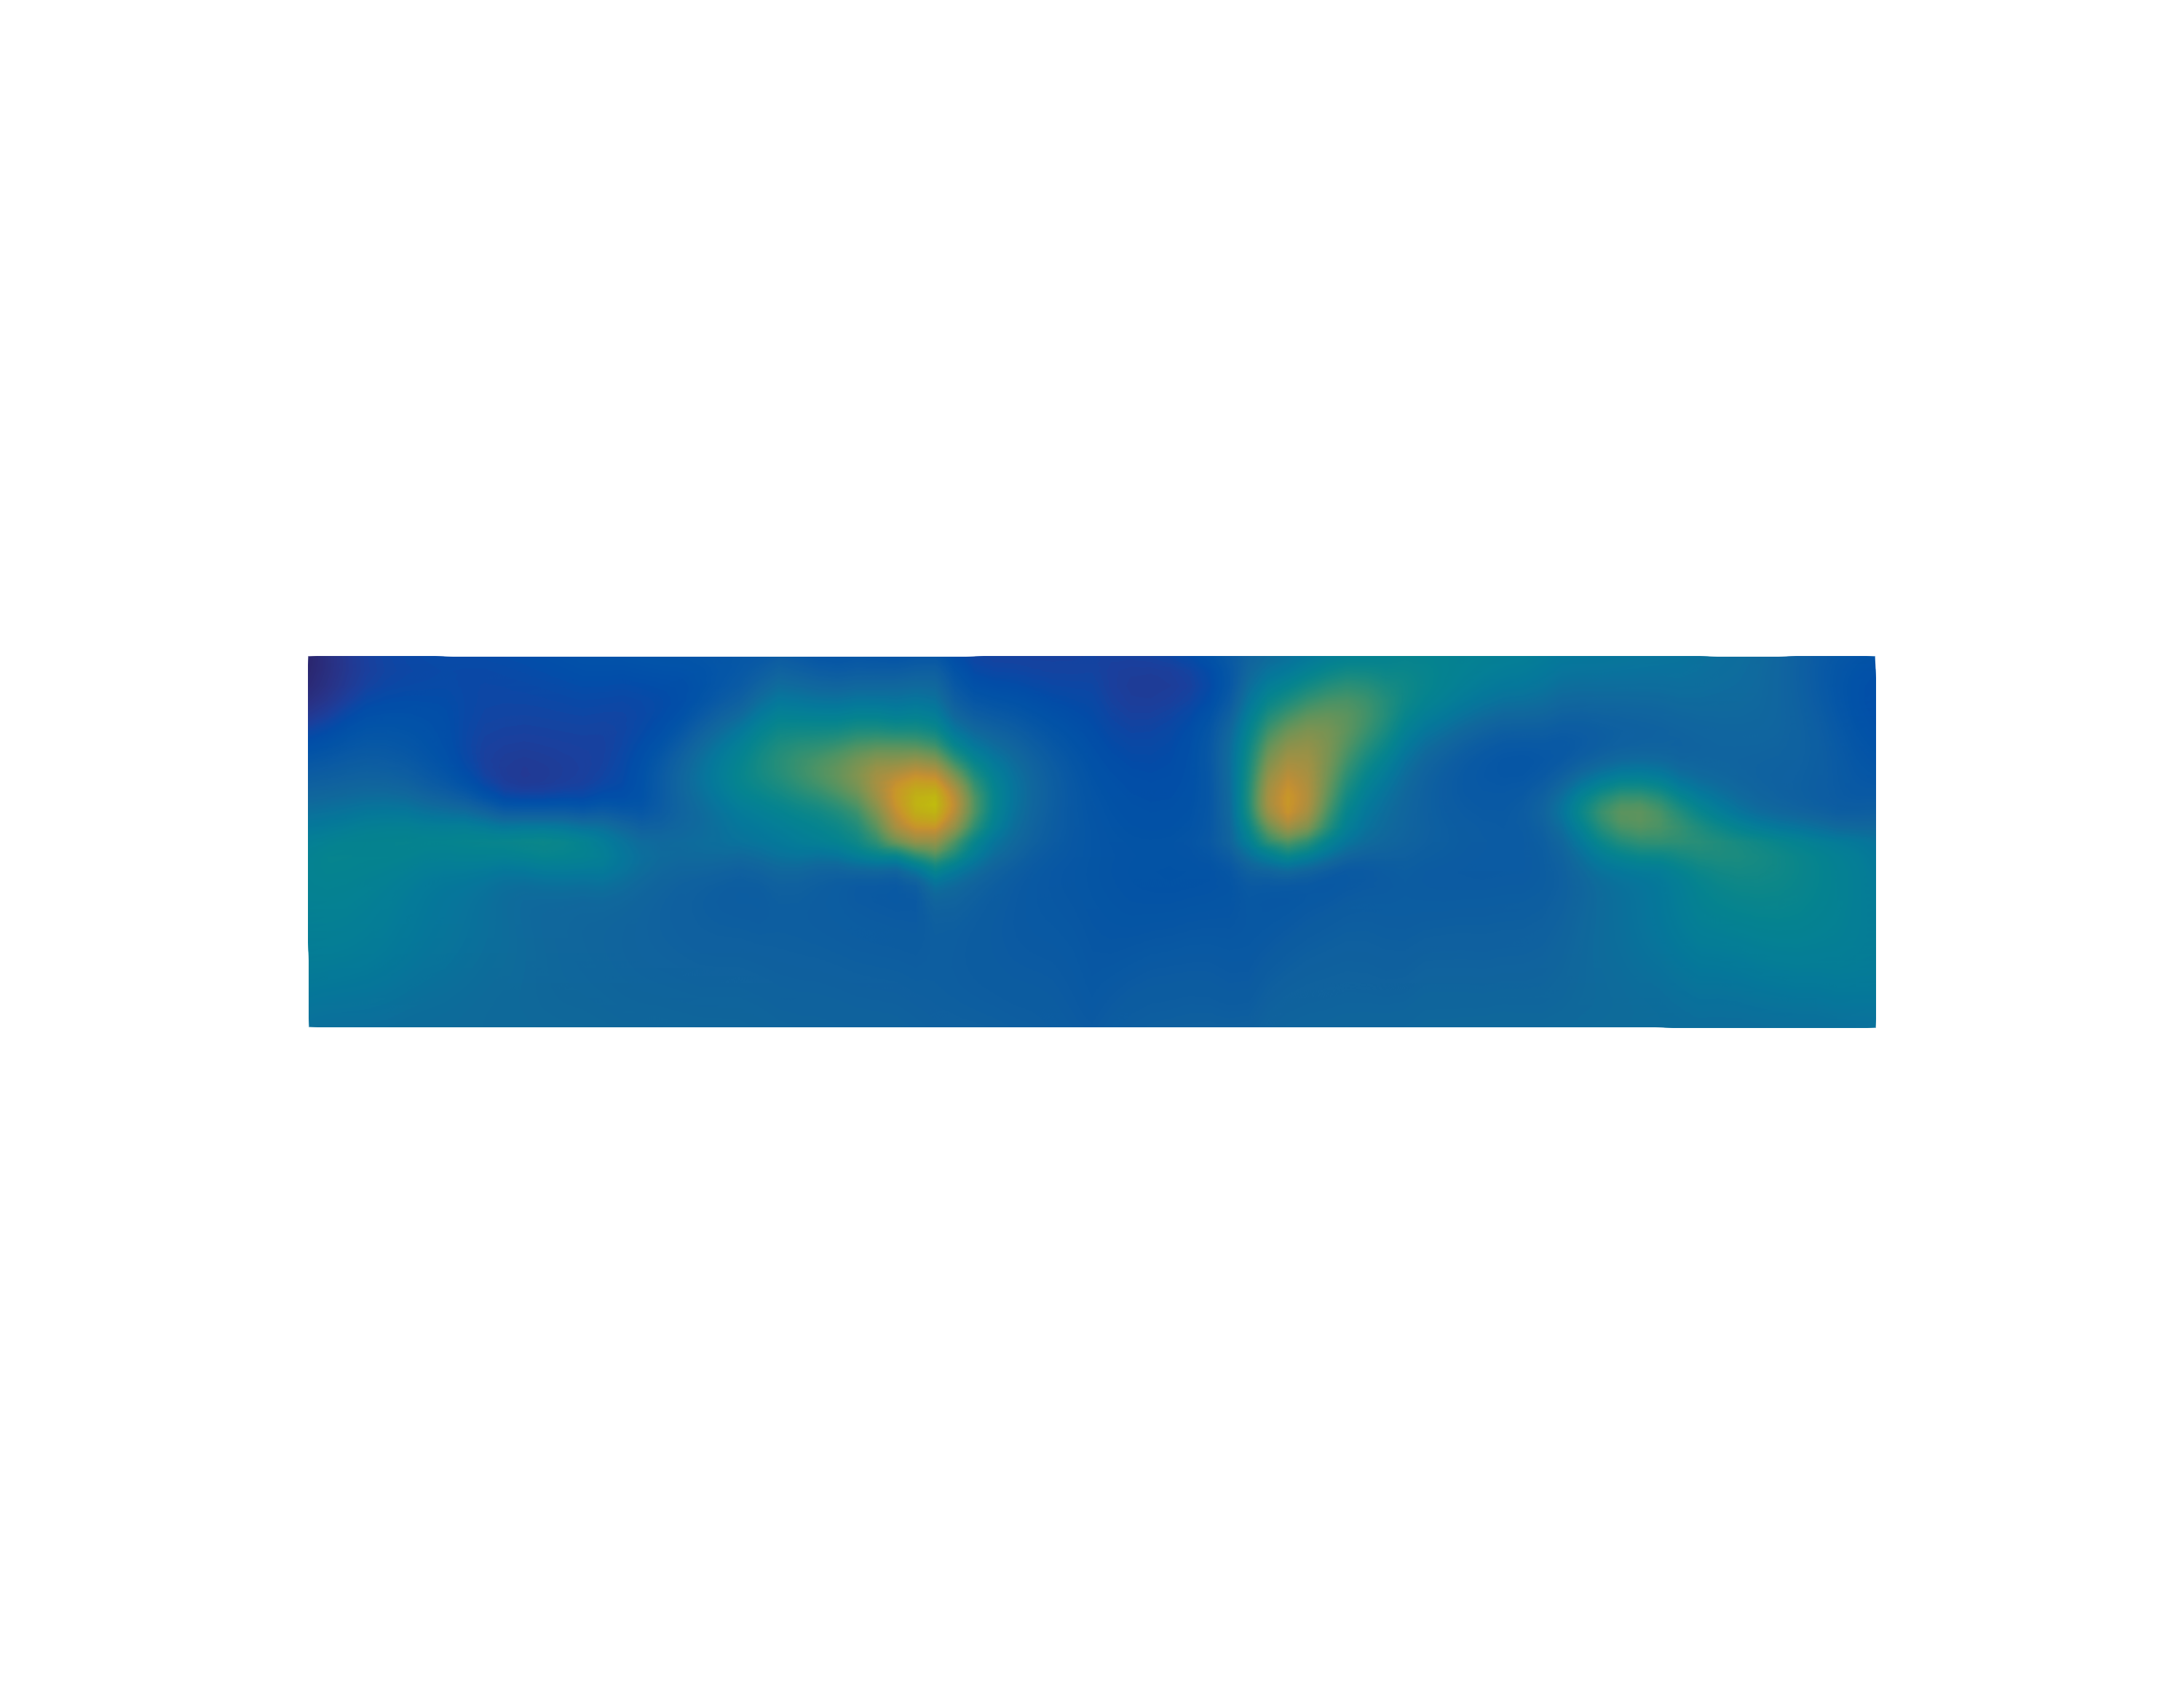
\includegraphics[width=0.9\textwidth]{../media/fourier/application/print/ab-0-1-concentration-acd.png}
        \caption{Anode $(1,1)$ désactivée}
      \end{center}
    \end{subfigure}
    \begin{subfigure}[t]{\textwidth}
      \begin{center}
        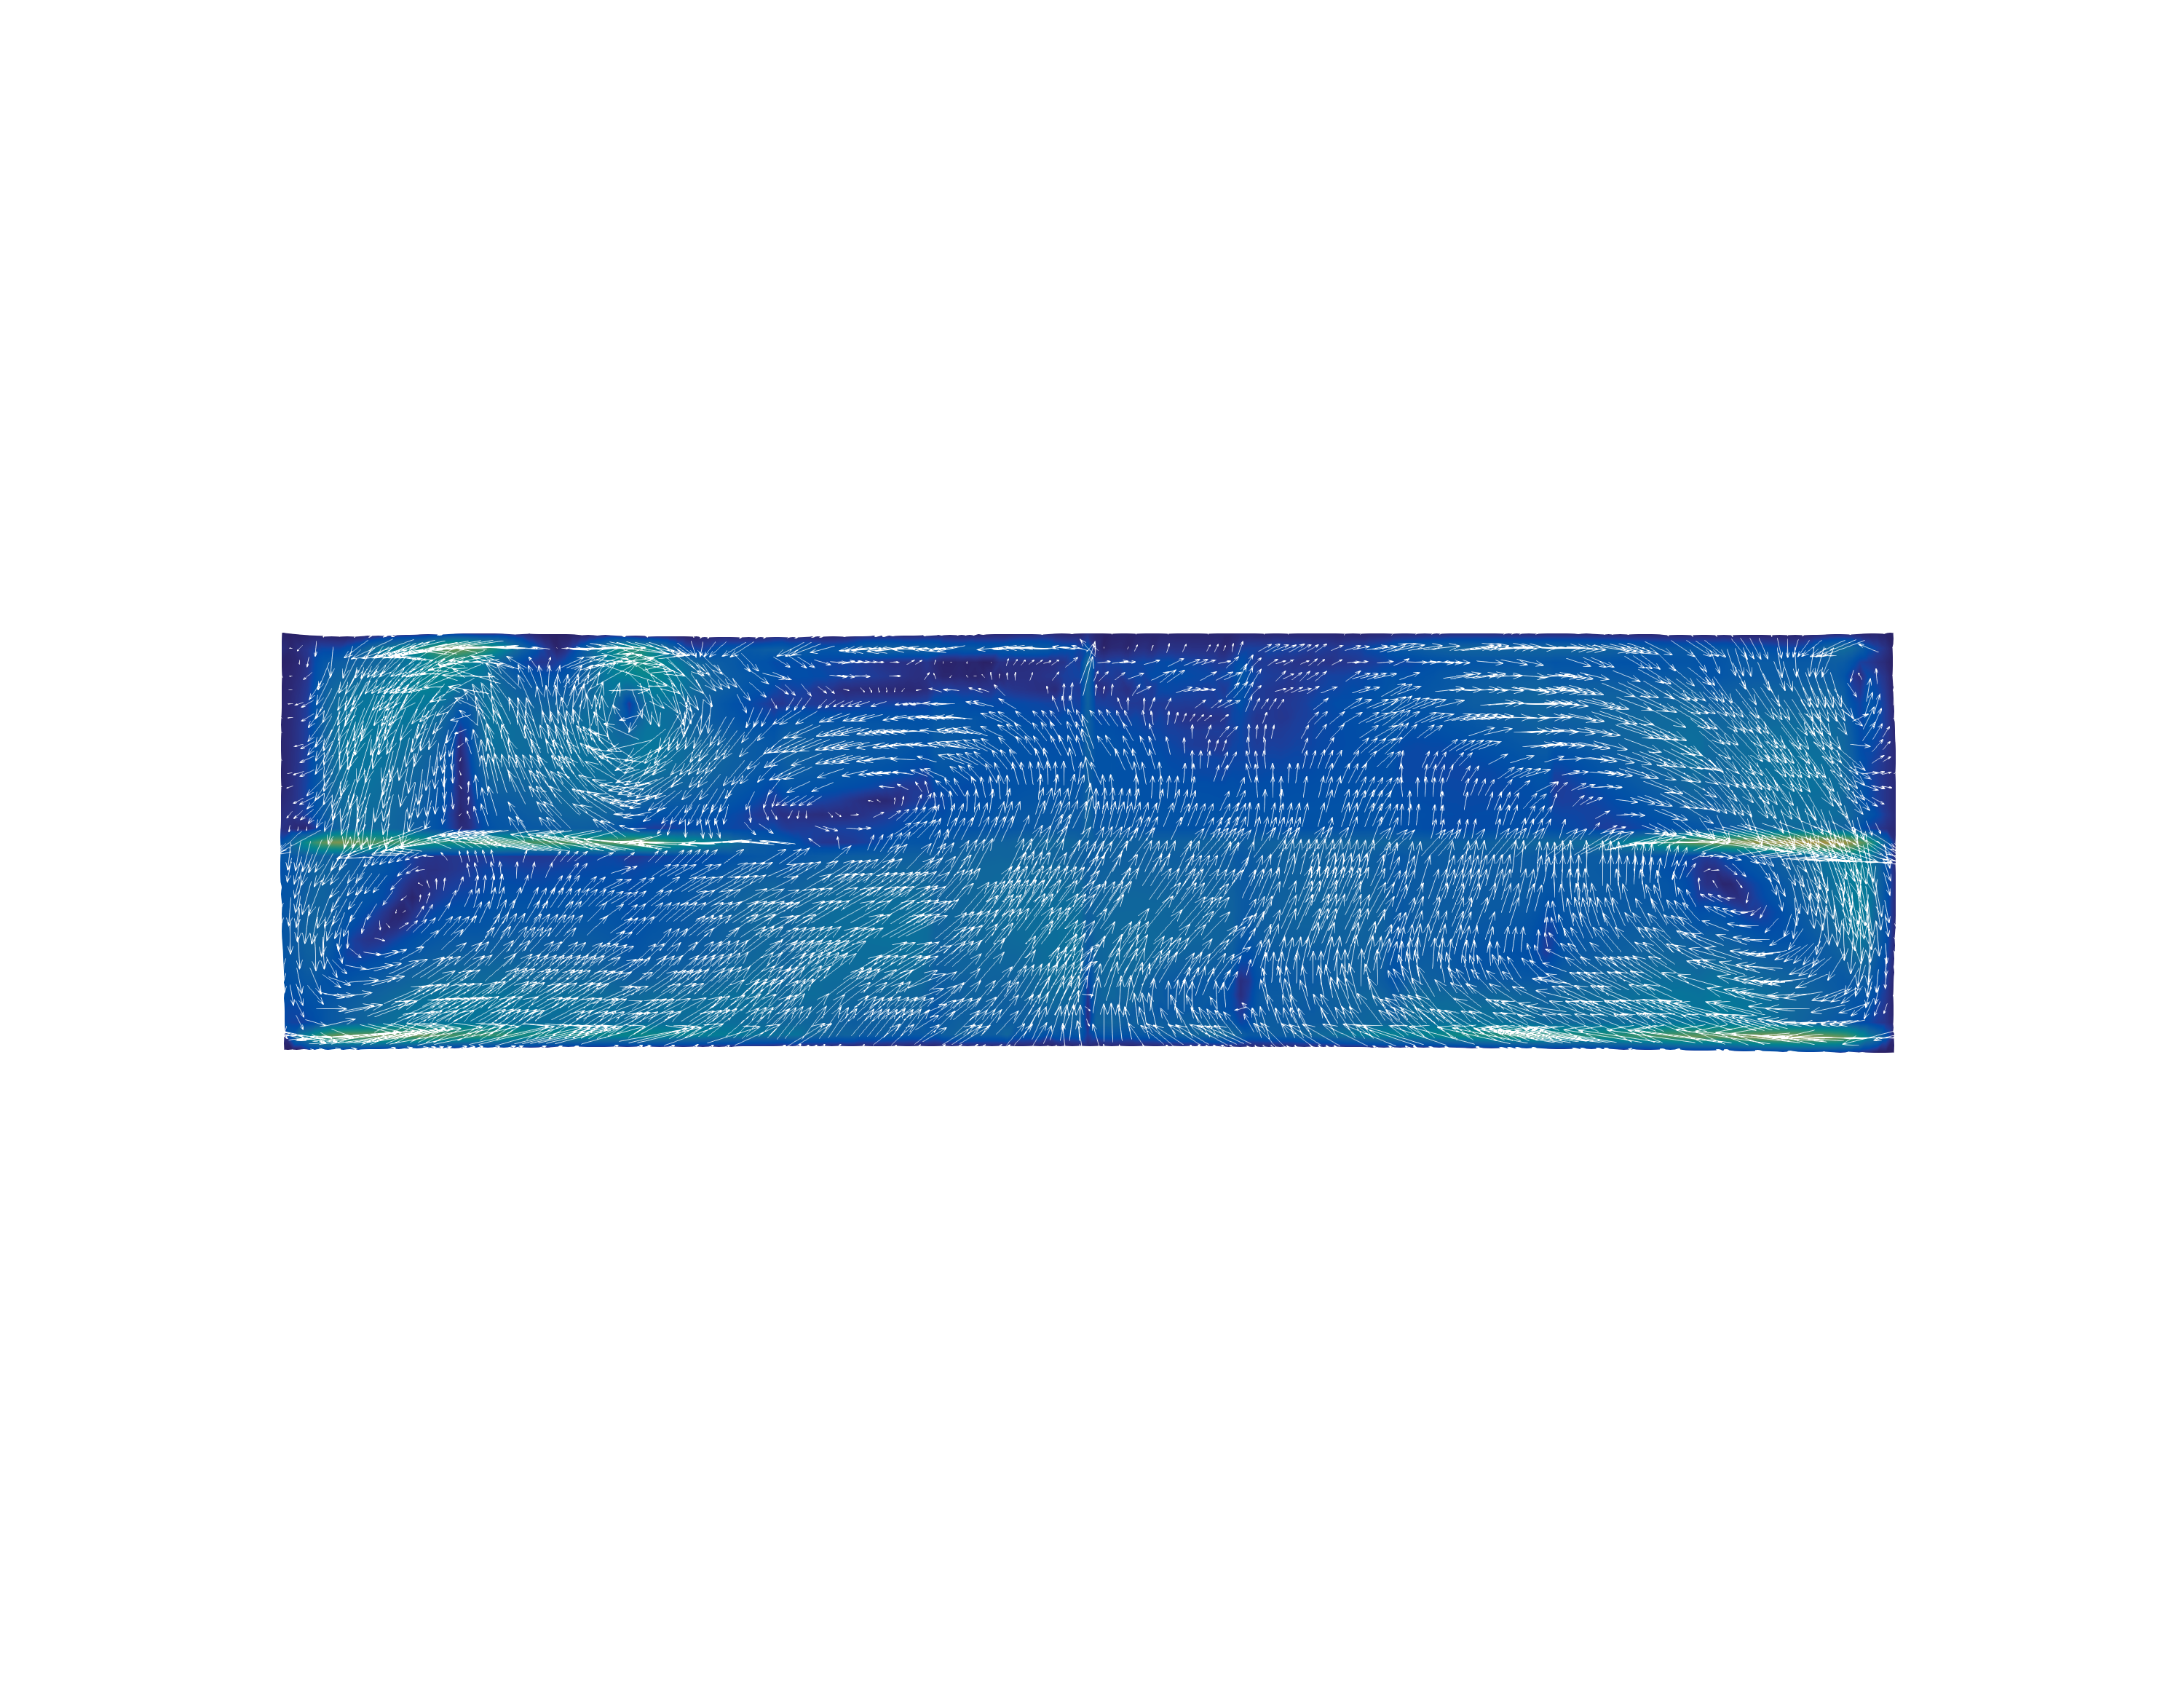
\includegraphics[width=0.9\textwidth]{../media/fourier/application/print/ab-0-2-velocity-acd.png}
        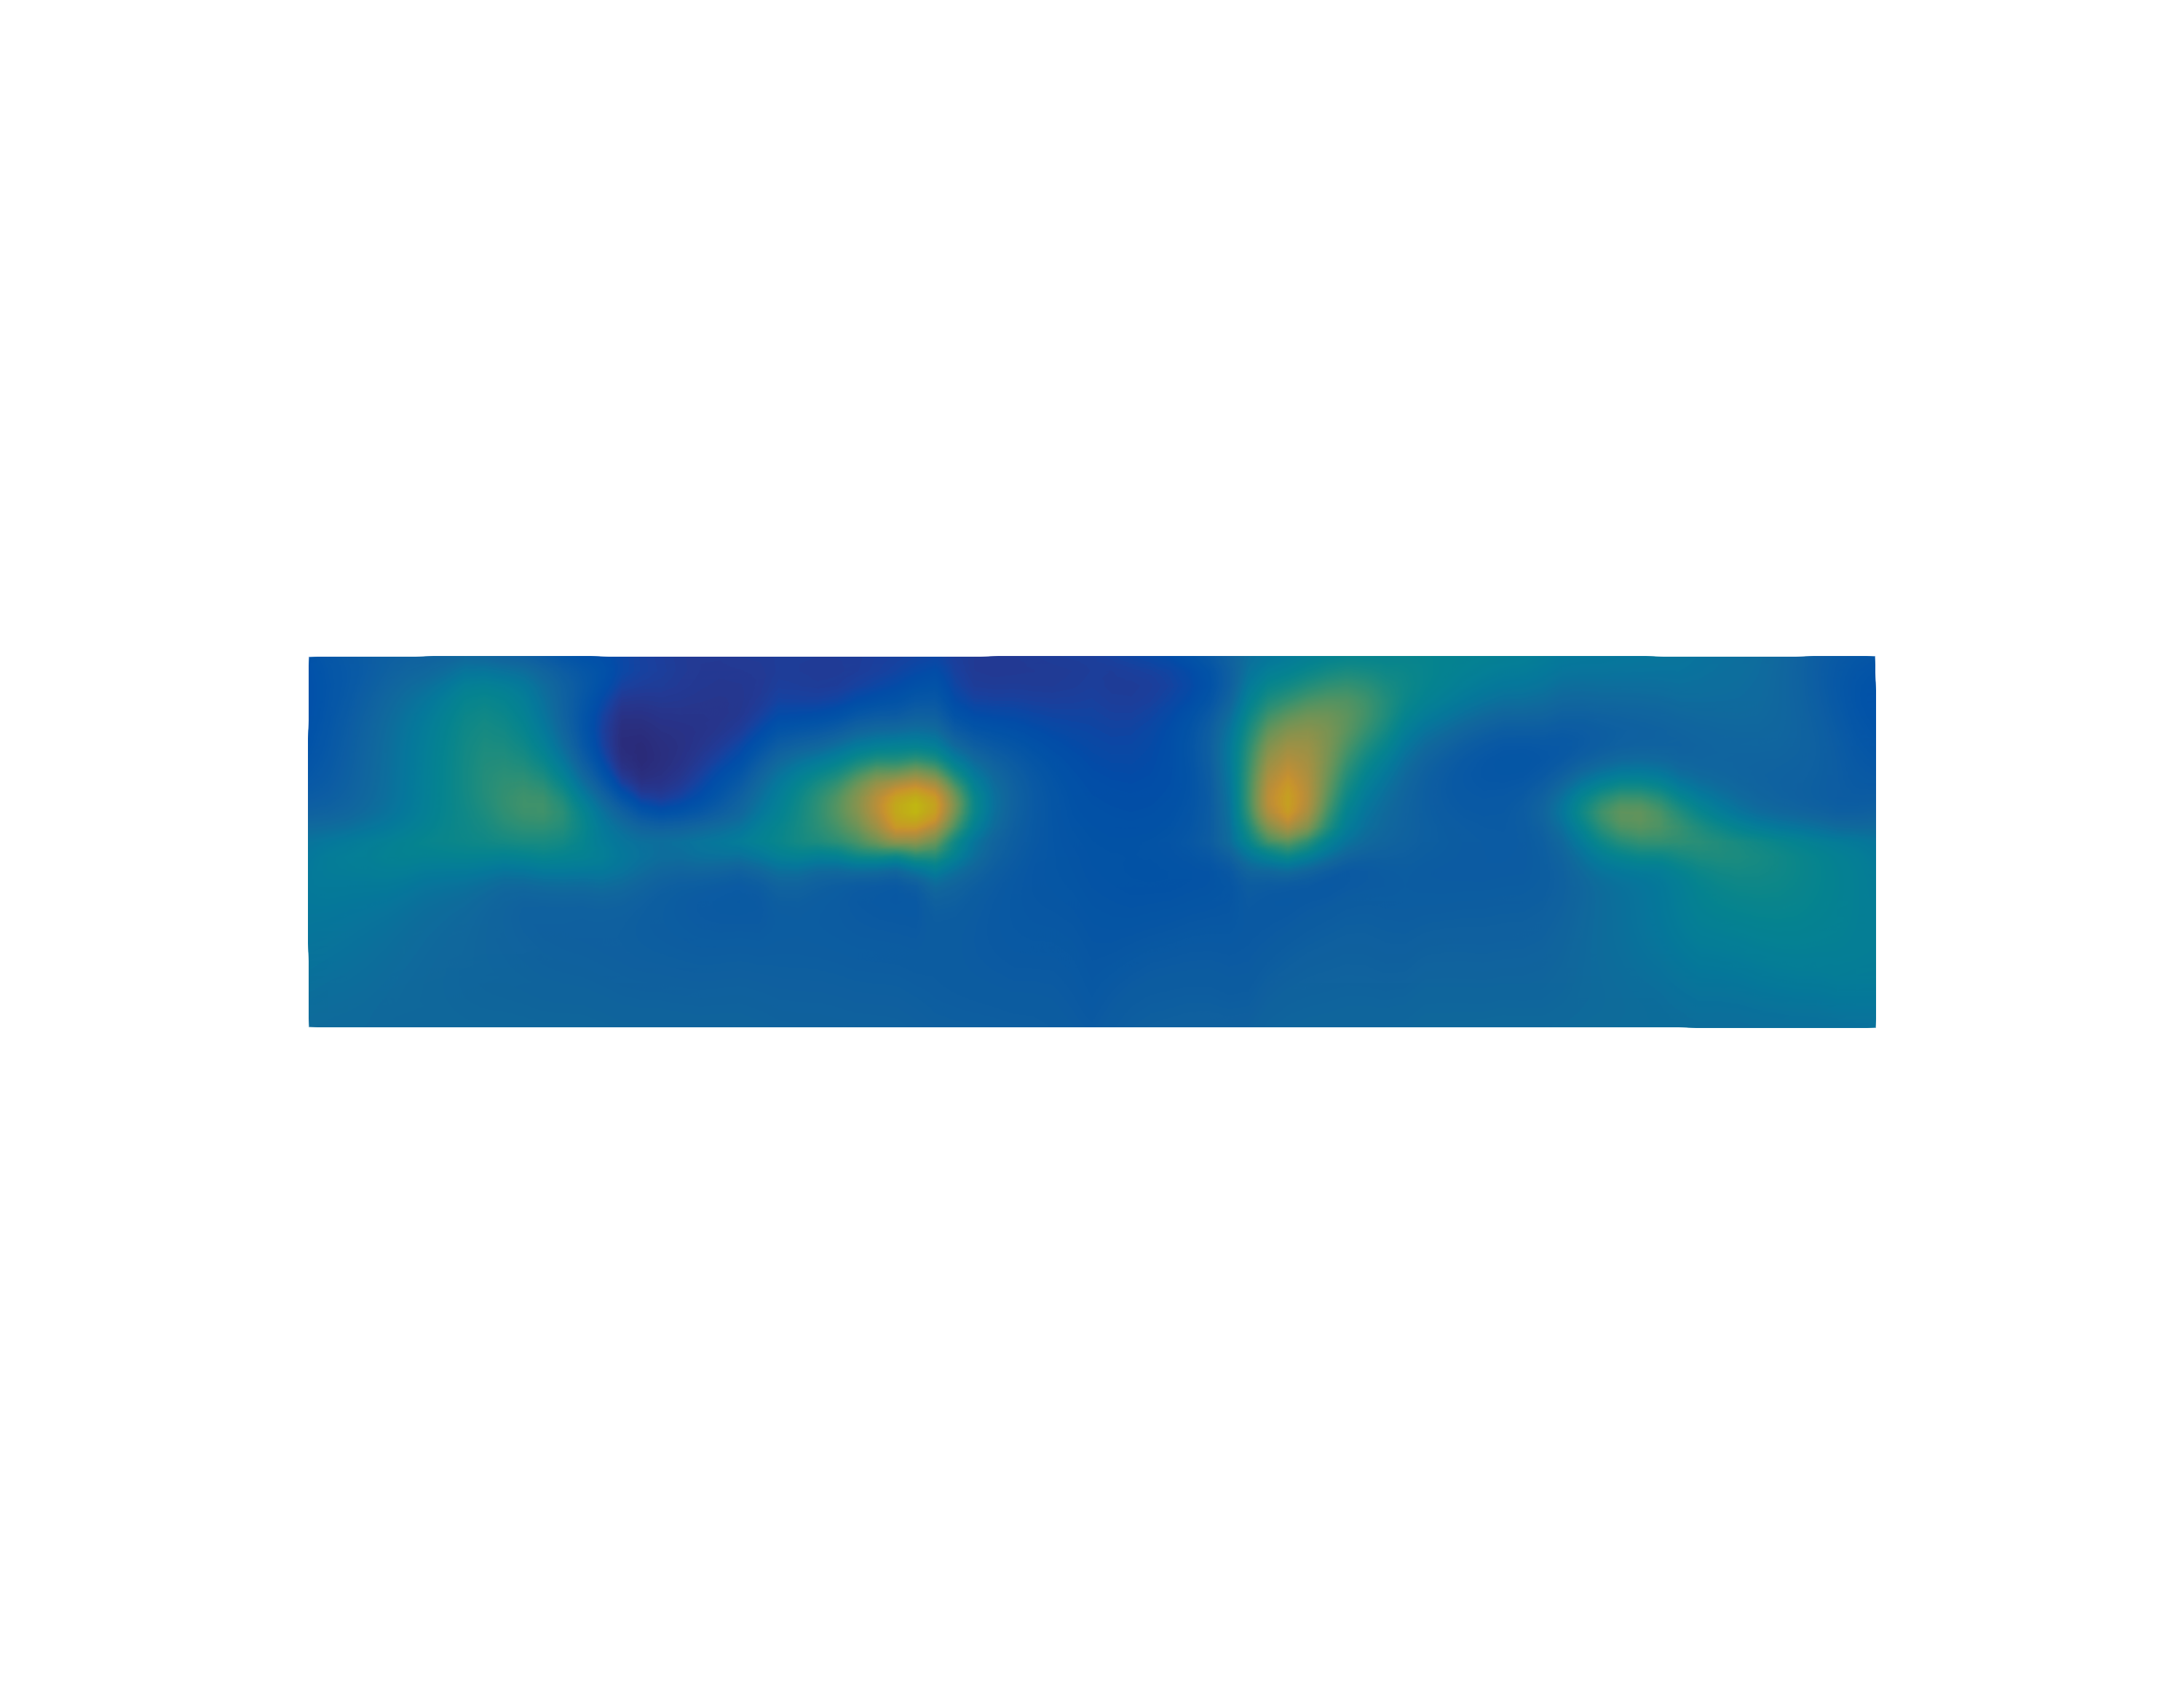
\includegraphics[width=0.9\textwidth]{../media/fourier/application/print/ab-0-2-concentration-acd.png}
        \caption{Anode $(1,2)$ désactivée}
      \end{center}
    \end{subfigure}

    \begin{multicols}{2}
        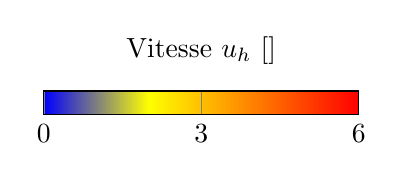
\begin{tikzpicture}
          \begin{axis}[
              colorbar,
              hide axis,
              scale only axis,
              height=0.10\textwidth,
              width=0.5\textwidth,
              colorbar horizontal,
              point meta min=0.0,
              point meta max=6.0,
              colorbar style={
                title=Vitesse $u_h$ [\si{\centi\meter\per\second}],
                width=4cm,
                height=0.3cm,
                xtick={0.0, 3.0, 6.0},
                at={(0.3\textwidth,0.4cm)},
                anchor=north
              }
            ]
            \addplot [] coordinates {(0,0)};
            \node (myfirstpic) at (0,0) {};
          \end{axis}
      \end{tikzpicture}\\
        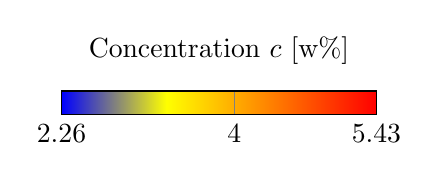
\begin{tikzpicture}
          \begin{axis}[
              colorbar,
              hide axis,
              scale only axis,
              height=0.10\textwidth,
              width=0.5\textwidth,
              colorbar horizontal,
              point meta min=2.26,
              point meta max=5.43,
              colorbar style={
                title=Concentration $c$ [w\%],
                width=4cm,
                height=0.3cm,
                xtick={2.26, 4, 5.43},
                at={(0.3\textwidth,0.4cm)},
                anchor=north
              }
            ]
            \addplot [] coordinates {(0,0)};
            \node (myfirstpic) at (0,0) {};
          \end{axis}
        \end{tikzpicture}
    \end{multicols}

    \caption{Champs de vitesse stationnaire $u^{\mathrm{S3D}}$ (haut) et de
      concentration $c^\mathrm{S3D}$ (bas) dans l'ACD de la cuve
      AP32 pour différentes configurations du plan anodique.}
    \label{fig:f3d-deactivated-a}
  \end{center}
\end{figure}

\begin{figure}[!h]
  \begin{center}
    \begin{subfigure}[t]{\textwidth}
      \begin{center}
        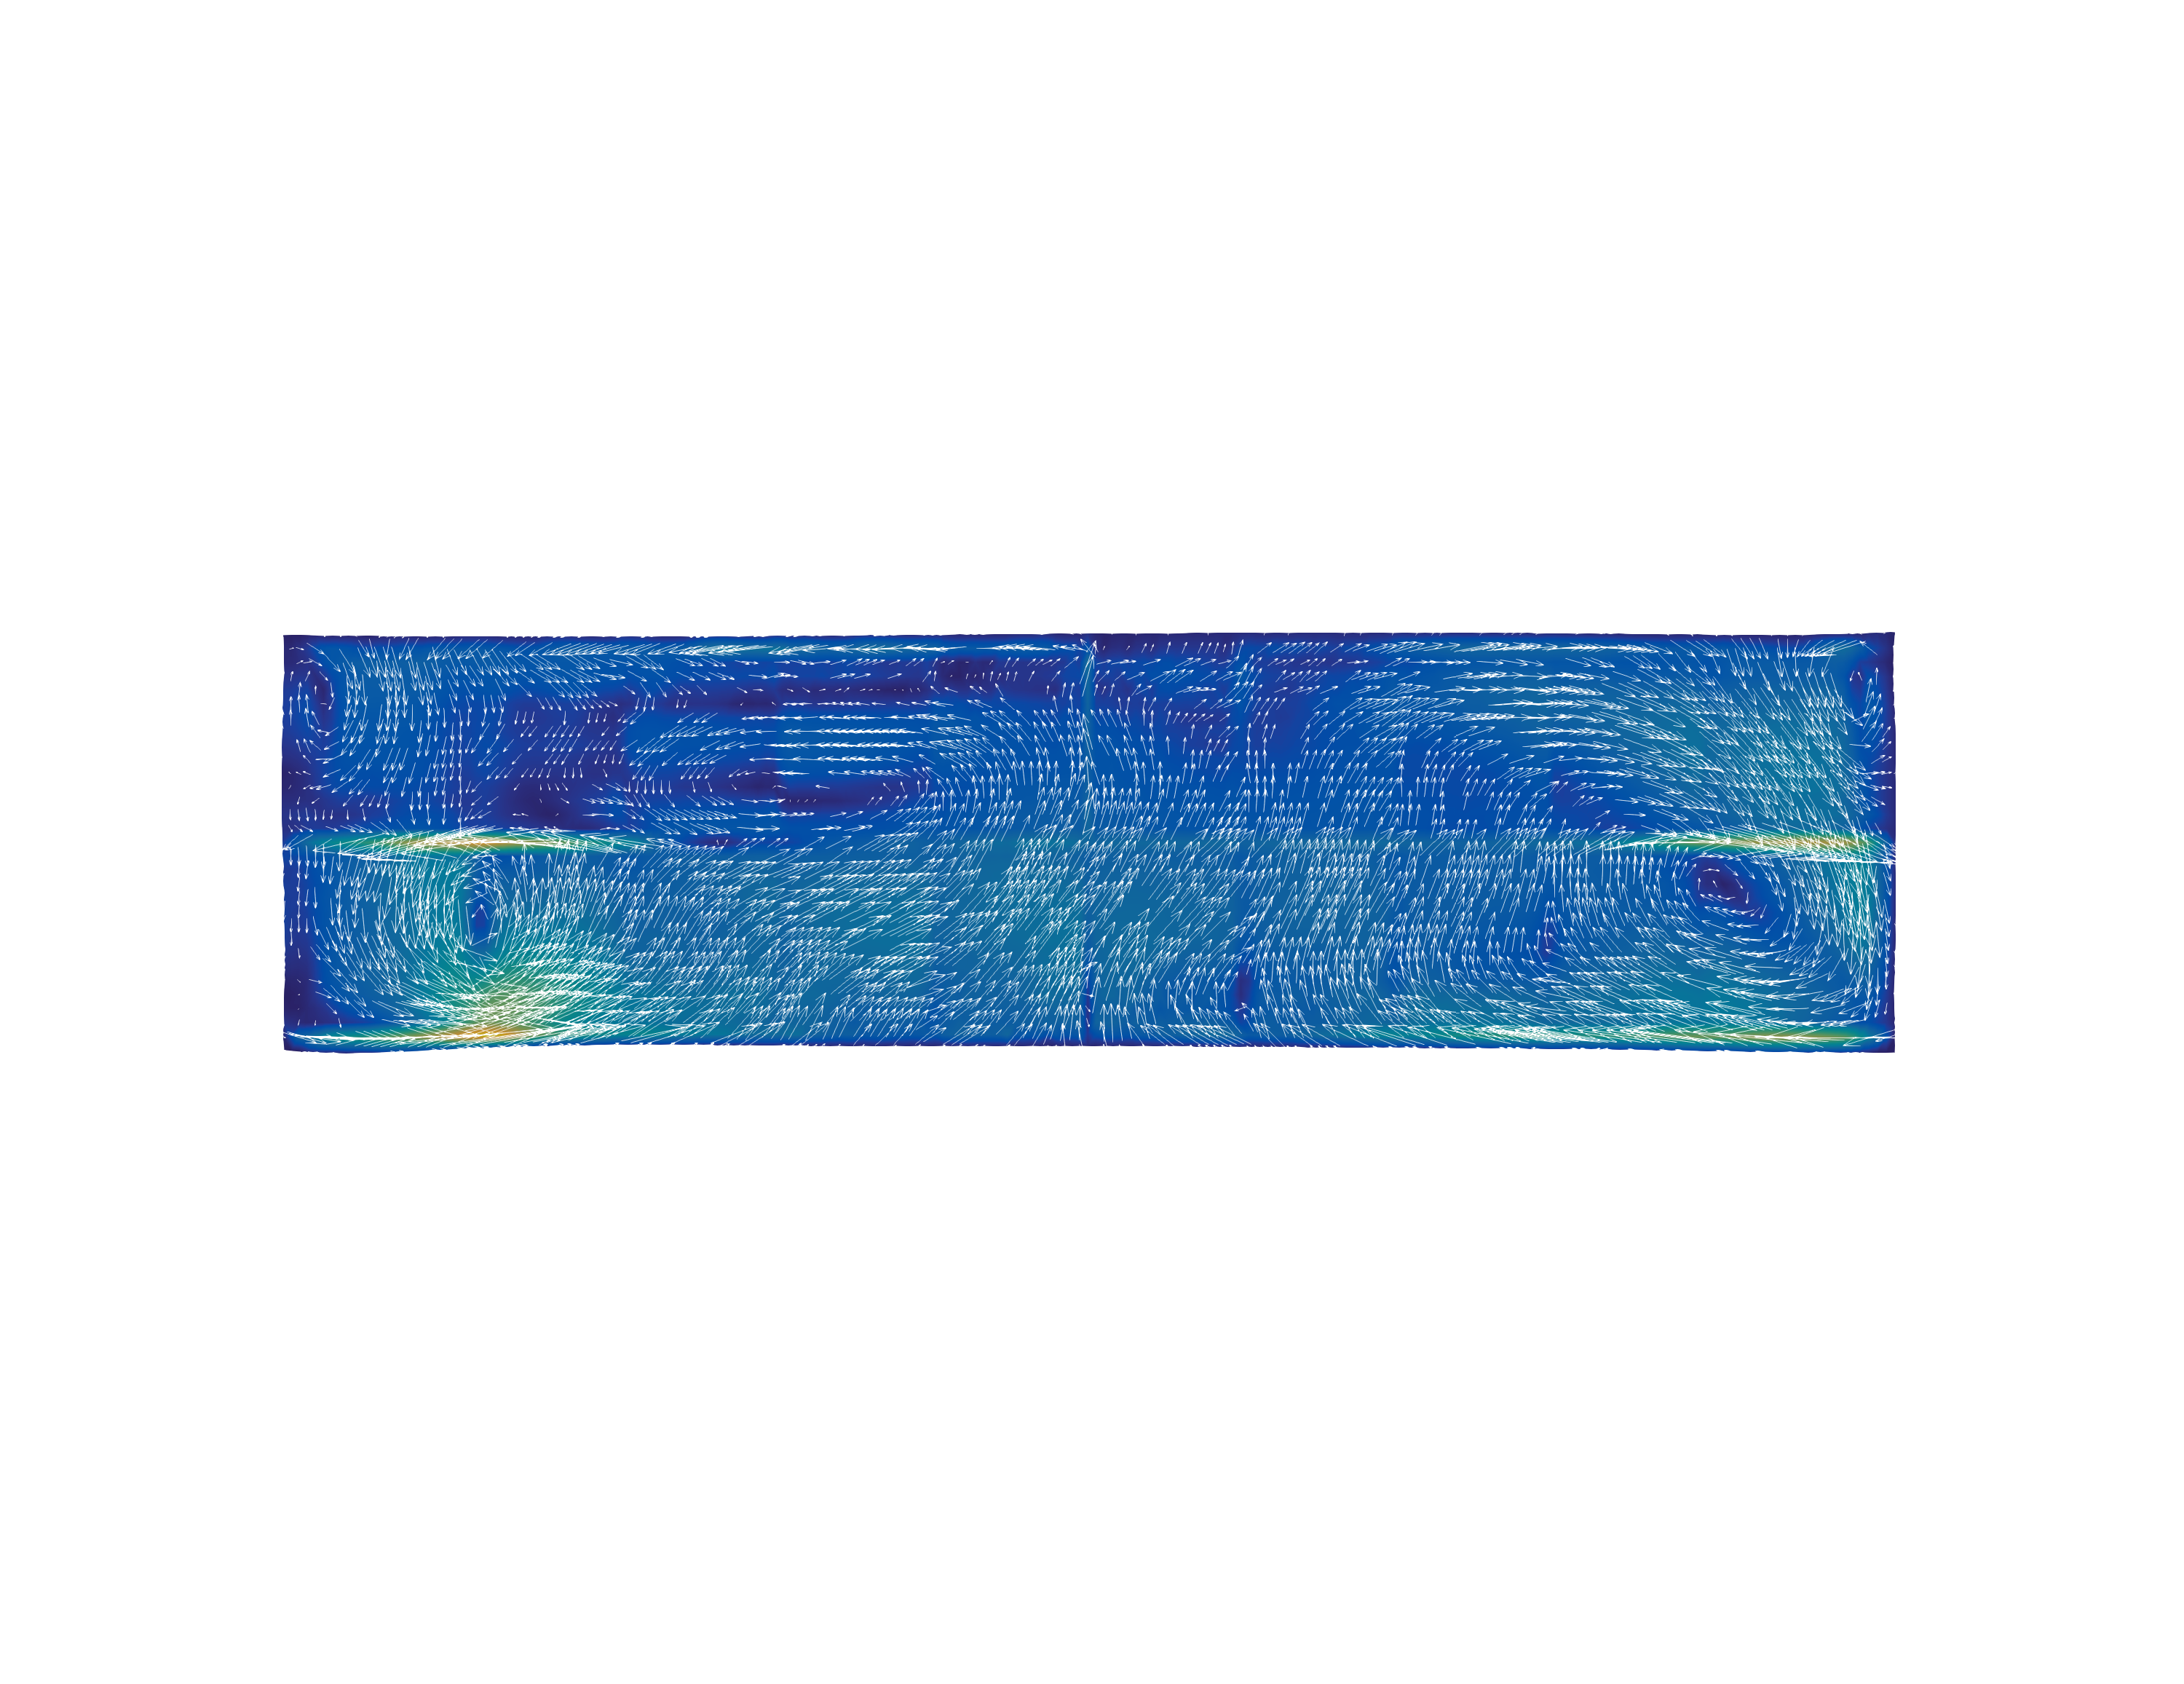
\includegraphics[width=0.9\textwidth]{../media/fourier/application/print/ab-1-1-velocity-acd.png}
        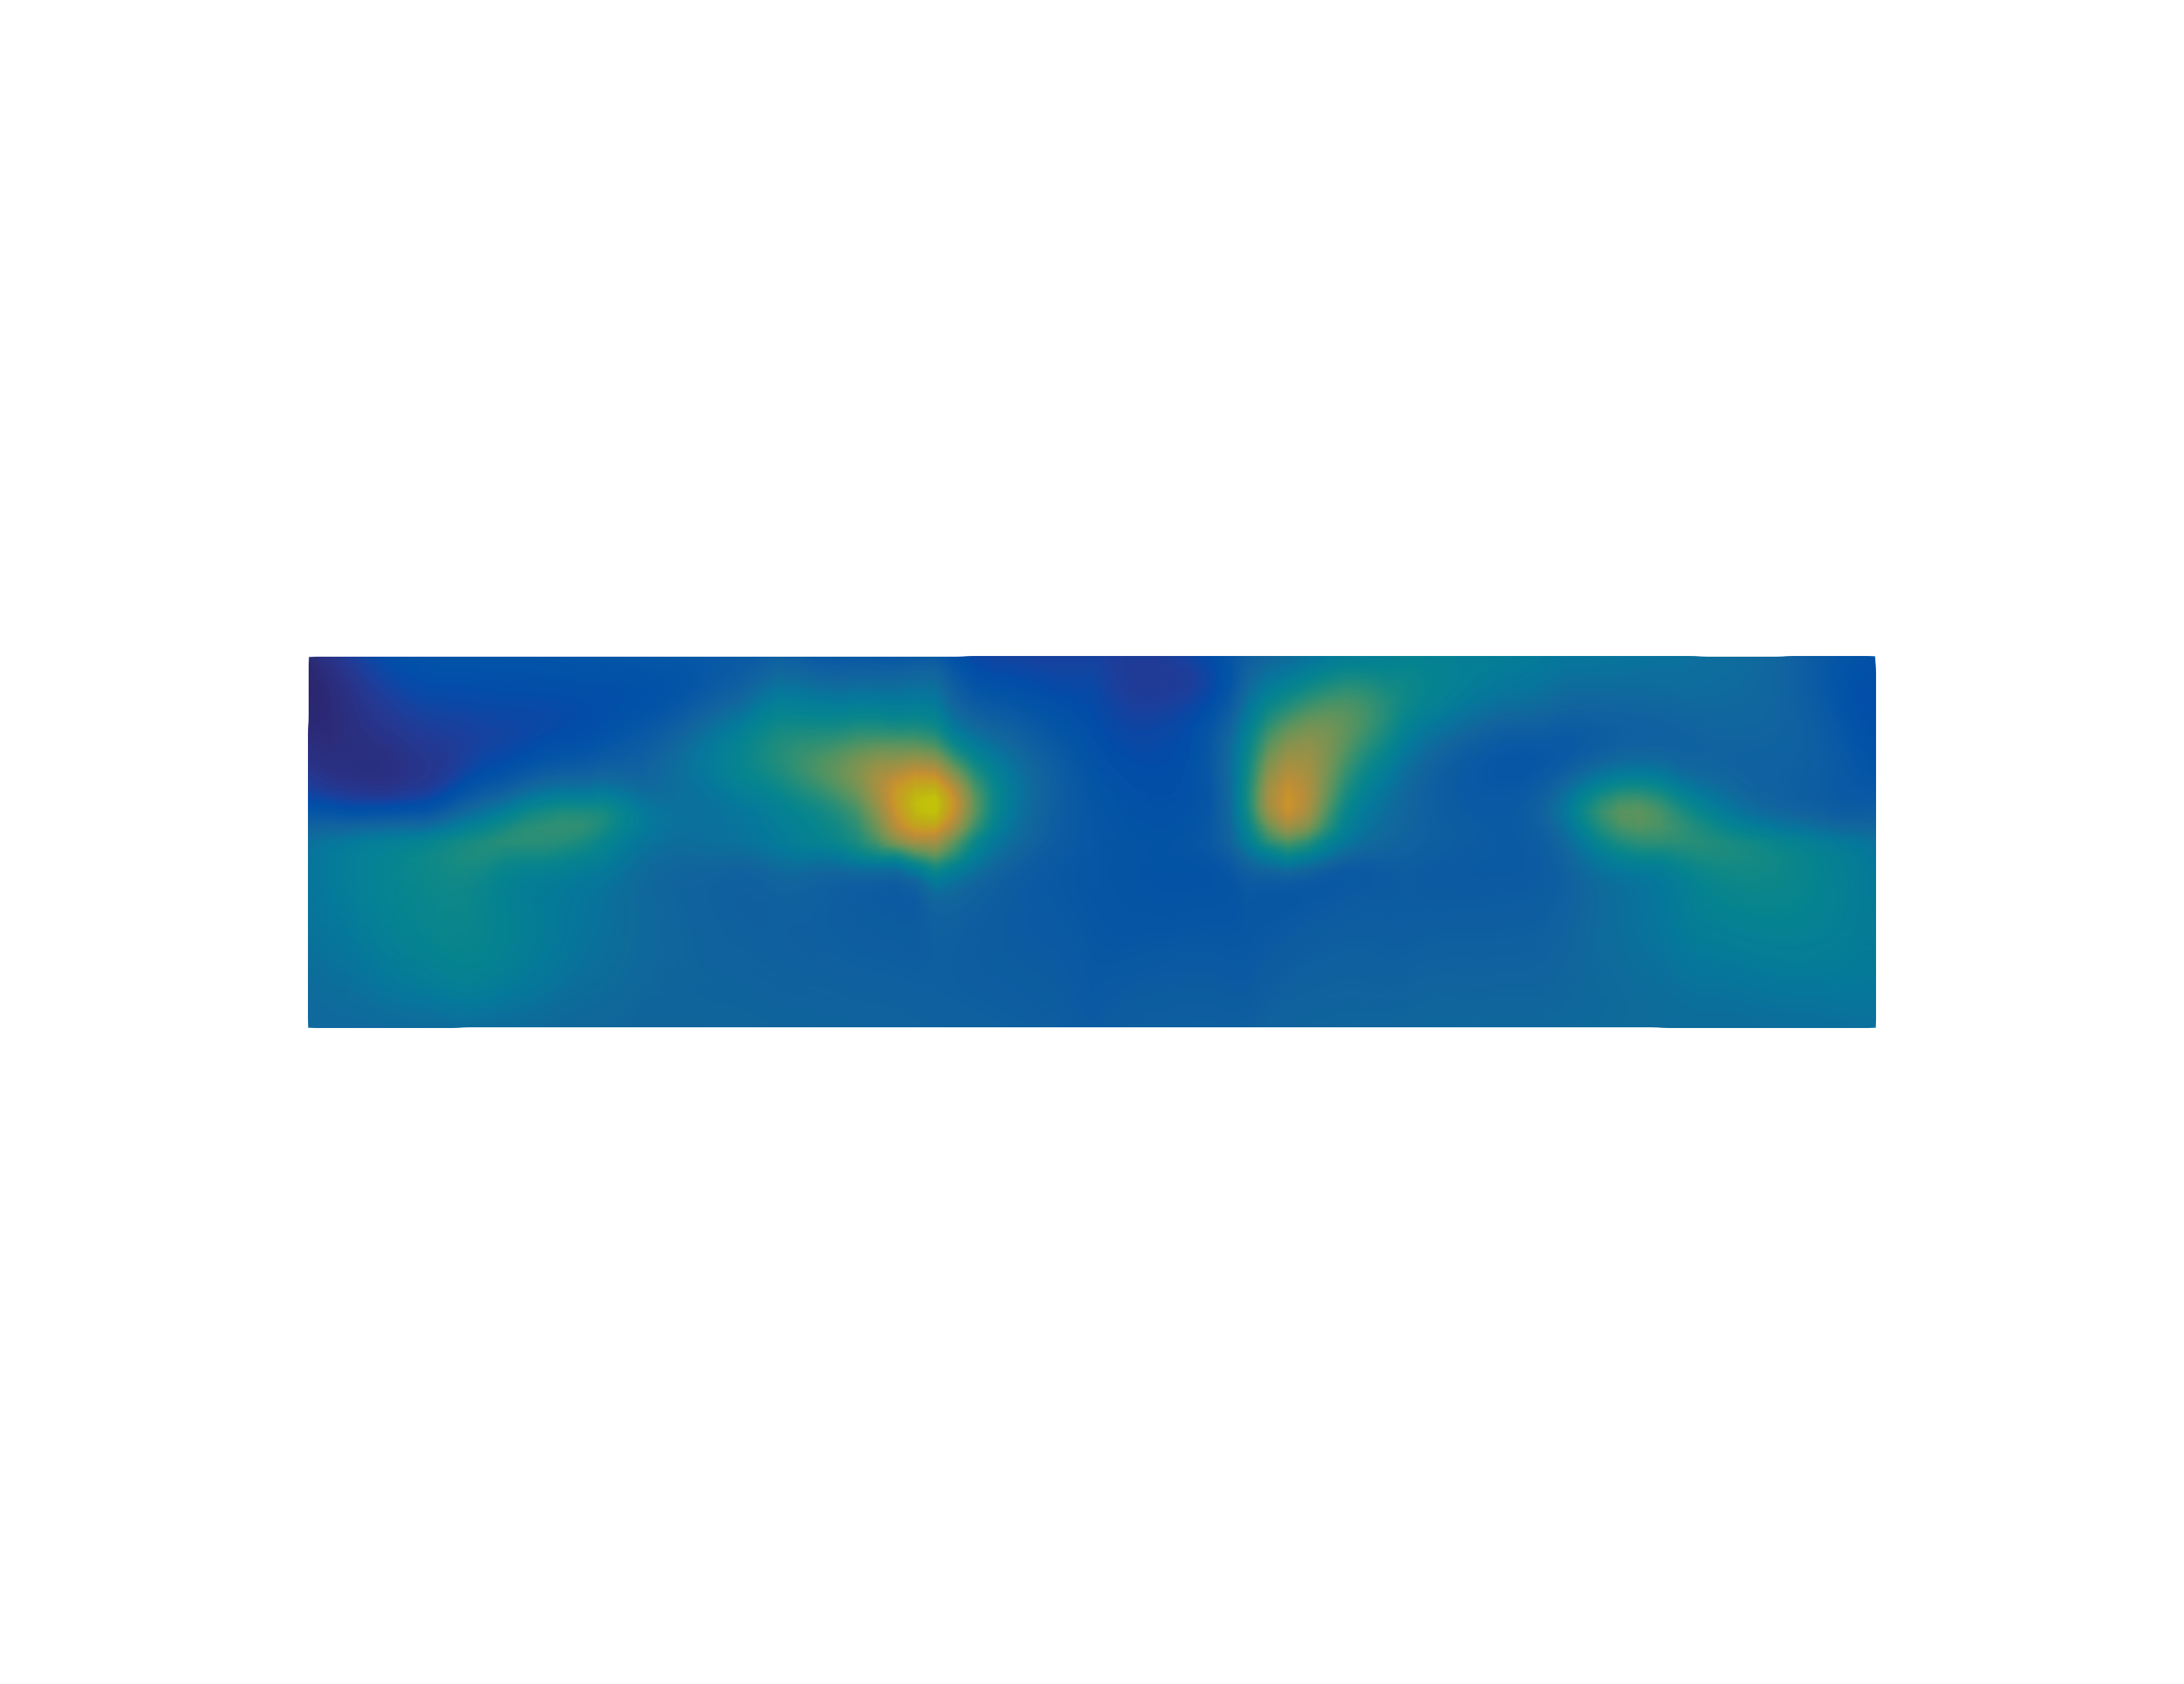
\includegraphics[width=0.9\textwidth]{../media/fourier/application/print/ab-1-1-concentration-acd.png}
        \caption{Anode $(2,1)$ désactivée}
      \end{center}
    \end{subfigure}
    \begin{subfigure}[t]{\textwidth}
      \begin{center}
        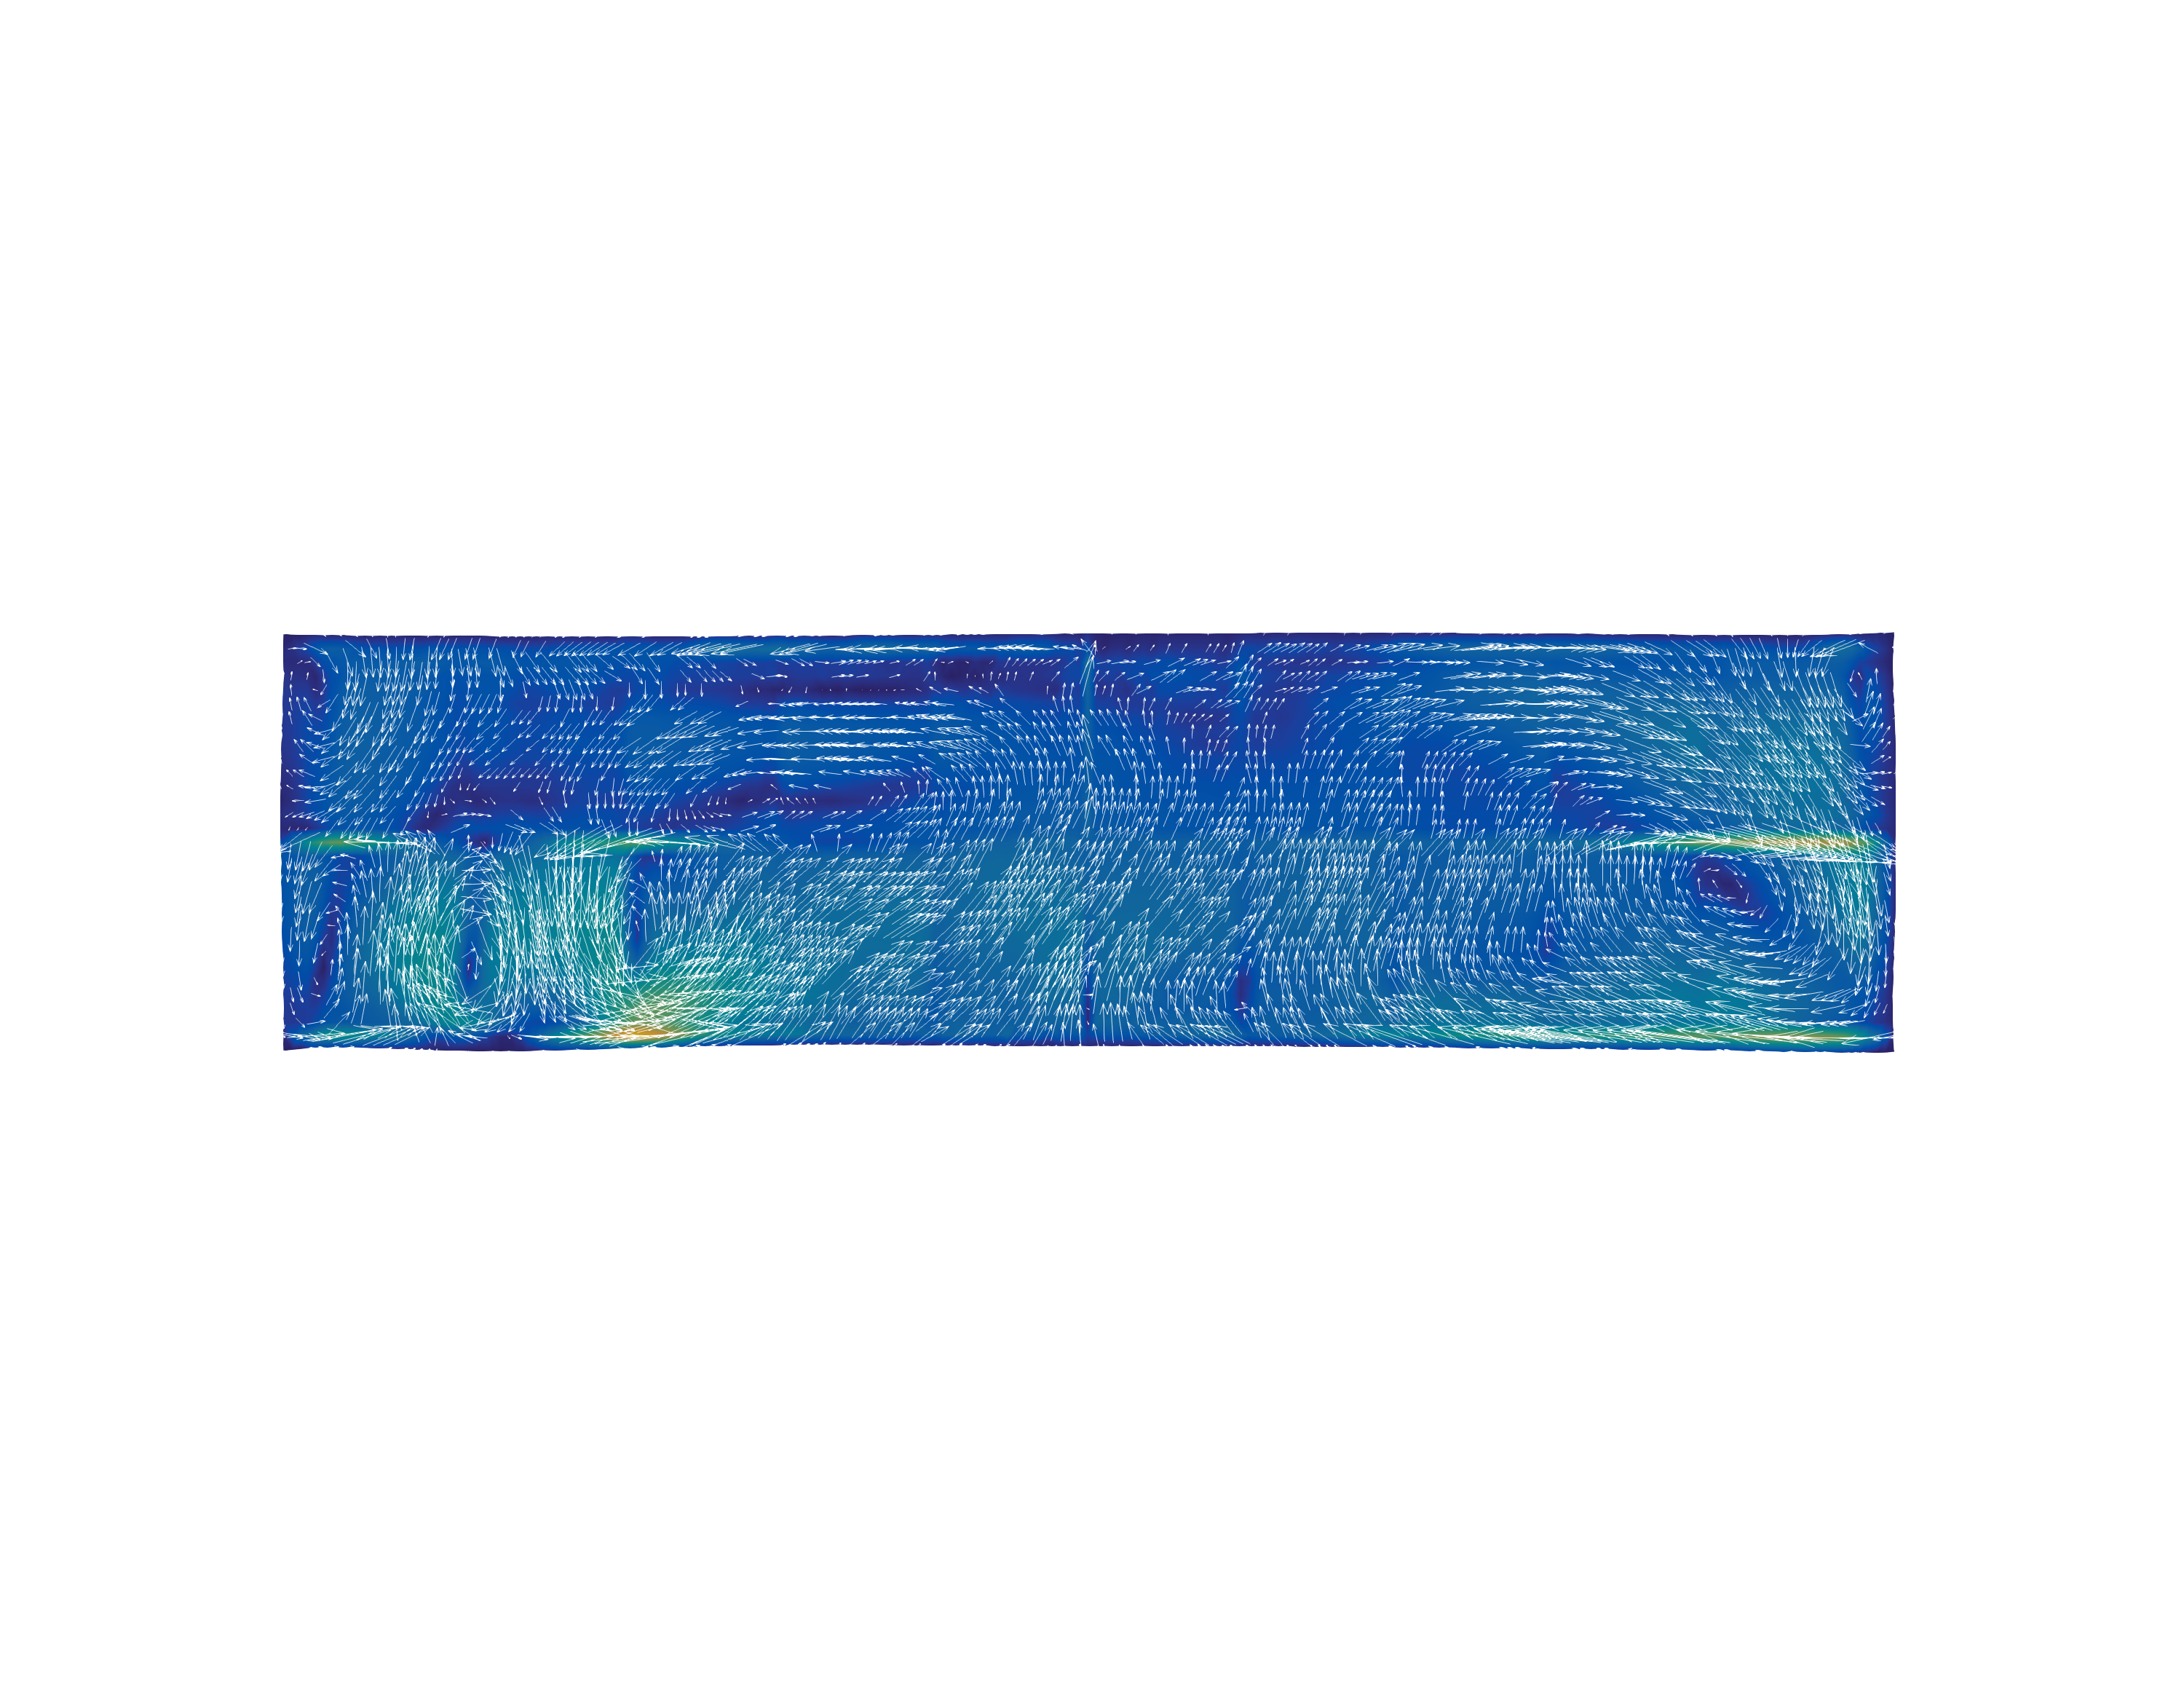
\includegraphics[width=0.9\textwidth]{../media/fourier/application/print/ab-1-2-velocity-acd.png}
        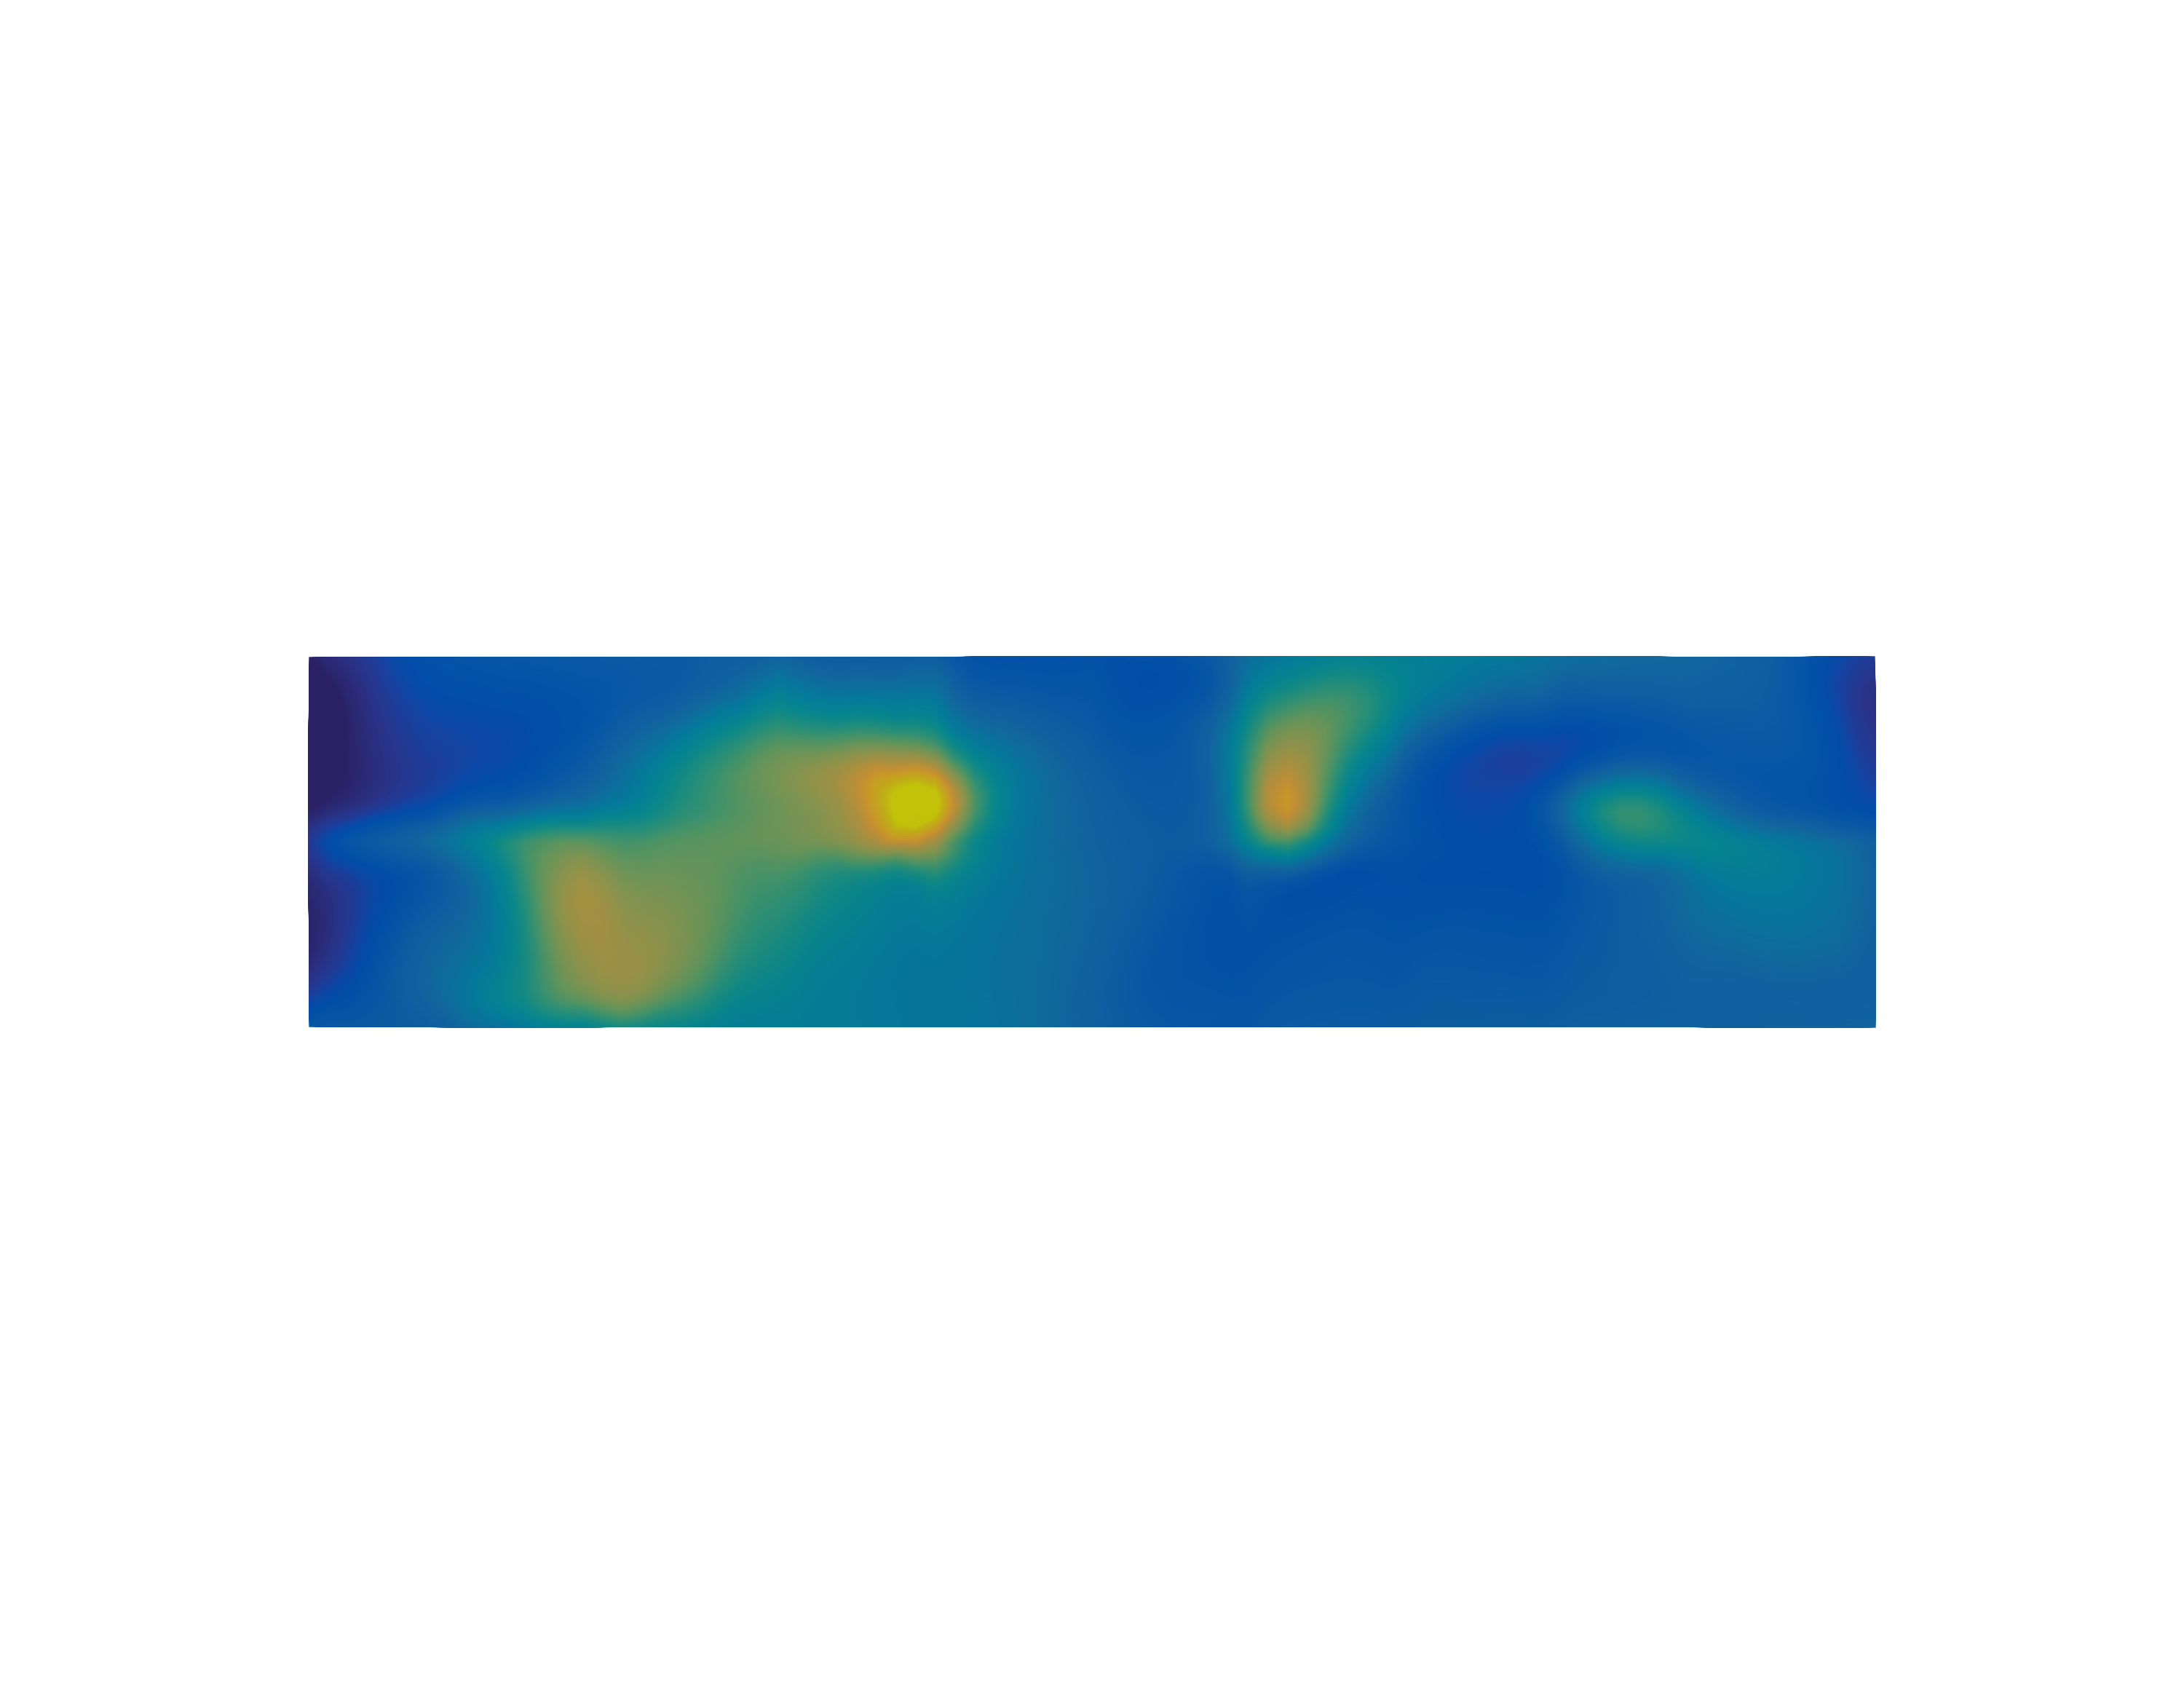
\includegraphics[width=0.9\textwidth]{../media/fourier/application/print/ab-1-2-concentration-acd.png}
        \caption{Anode $(2,2)$ désactivée}
      \end{center}
    \end{subfigure}

    \begin{multicols}{2}
        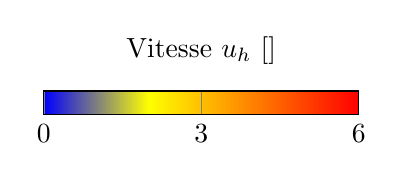
\begin{tikzpicture}
          \begin{axis}[
              colorbar,
              hide axis,
              scale only axis,
              height=0.10\textwidth,
              width=0.5\textwidth,
              colorbar horizontal,
              point meta min=0.0,
              point meta max=6.0,
              colorbar style={
                title=Vitesse $u_h$ [\si{\centi\meter\per\second}],
                width=4cm,
                height=0.3cm,
                xtick={0.0, 3.0, 6.0},
                at={(0.3\textwidth,0.4cm)},
                anchor=north
              }
            ]
            \addplot [] coordinates {(0,0)};
            \node (myfirstpic) at (0,0) {};
          \end{axis}
      \end{tikzpicture}\\
        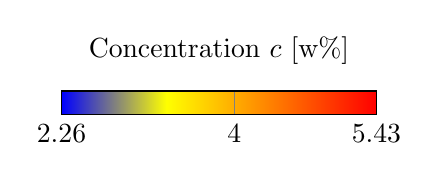
\begin{tikzpicture}
          \begin{axis}[
              colorbar,
              hide axis,
              scale only axis,
              height=0.10\textwidth,
              width=0.5\textwidth,
              colorbar horizontal,
              point meta min=2.26,
              point meta max=5.43,
              colorbar style={
                title=Concentration $c$ [w\%],
                width=4cm,
                height=0.3cm,
                xtick={2.26, 4, 5.43},
                at={(0.3\textwidth,0.4cm)},
                anchor=north
              }
            ]
            \addplot [] coordinates {(0,0)};
            \node (myfirstpic) at (0,0) {};
          \end{axis}
        \end{tikzpicture}
    \end{multicols}

    \caption{Champs de vitesse stationnaire $u^{\mathrm{S3D}}$ (haut) et de
      concentration $c^\mathrm{S3D}$ (bas) dans l'ACD de la cuve
      AP32 pour différentes configurations du plan anodique.}
    \label{fig:f3d-deactivated-b}
  \end{center}
\end{figure}
%


\begin{figure}[!h]
  \begin{center}
    \begin{subfigure}[t]{\textwidth}
      \begin{center}
        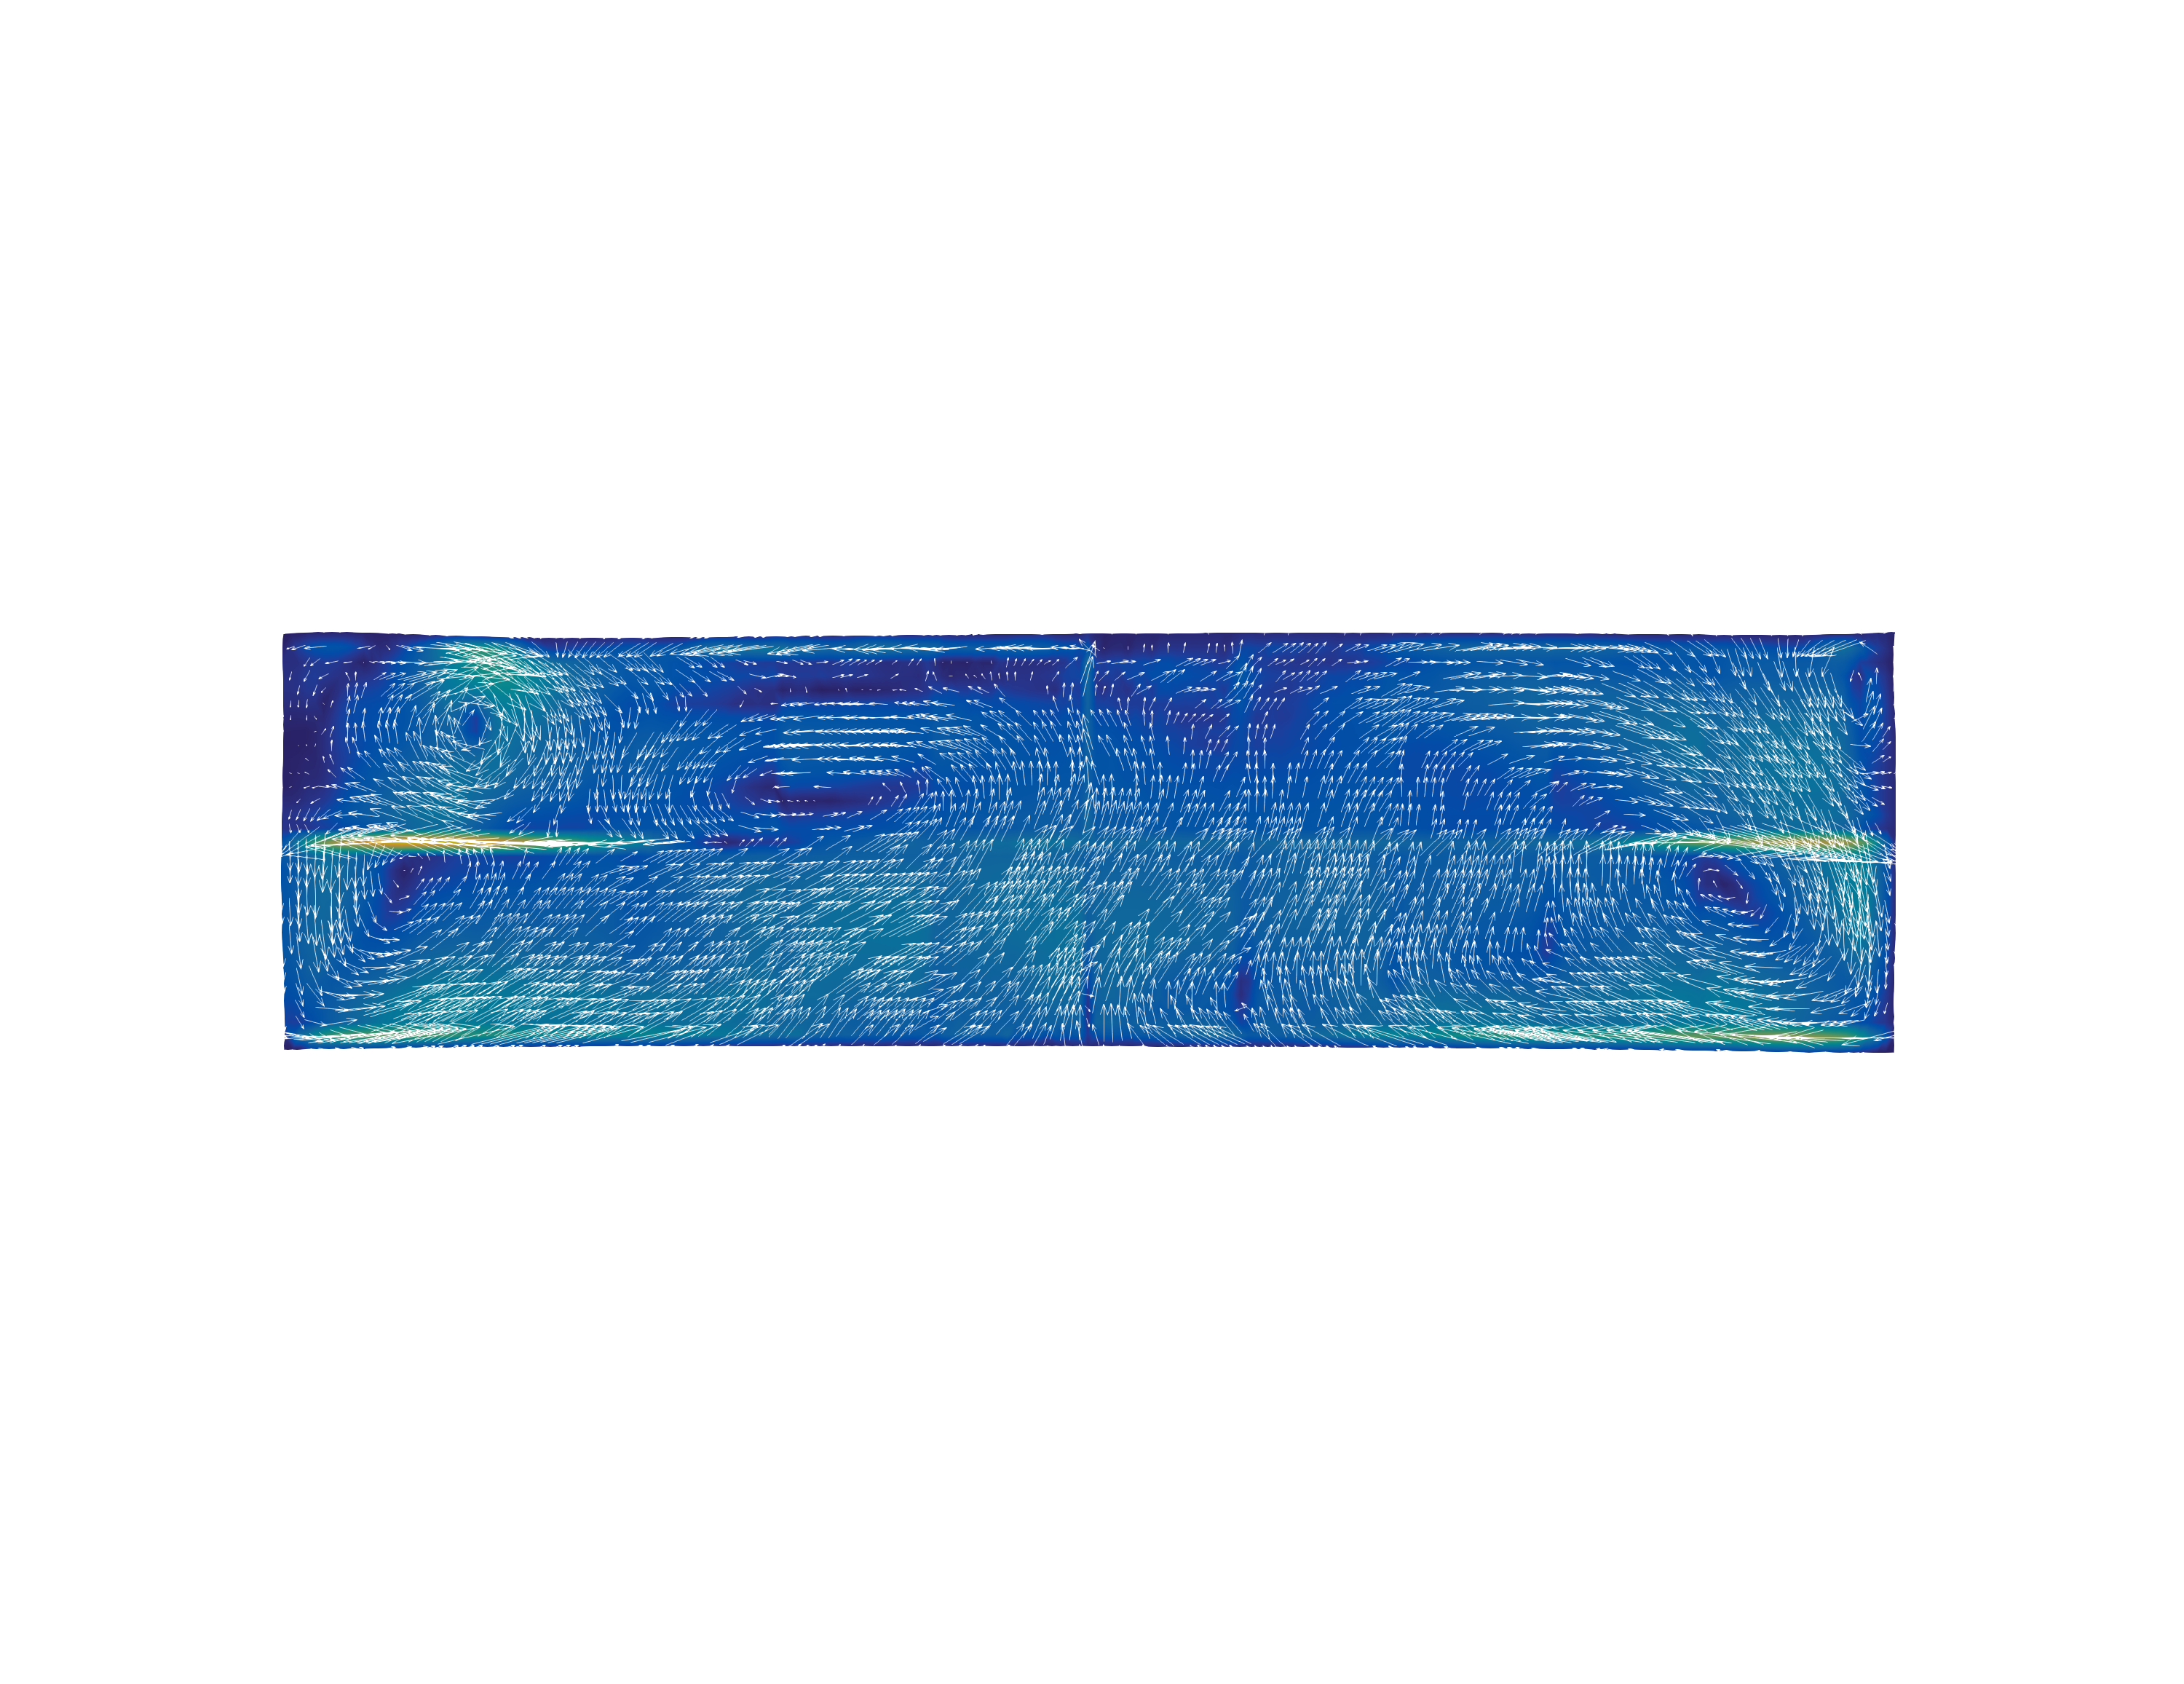
\includegraphics[width=0.9\textwidth]{../media/fourier/application/print/ab-0-1-velocity-acd.png}
        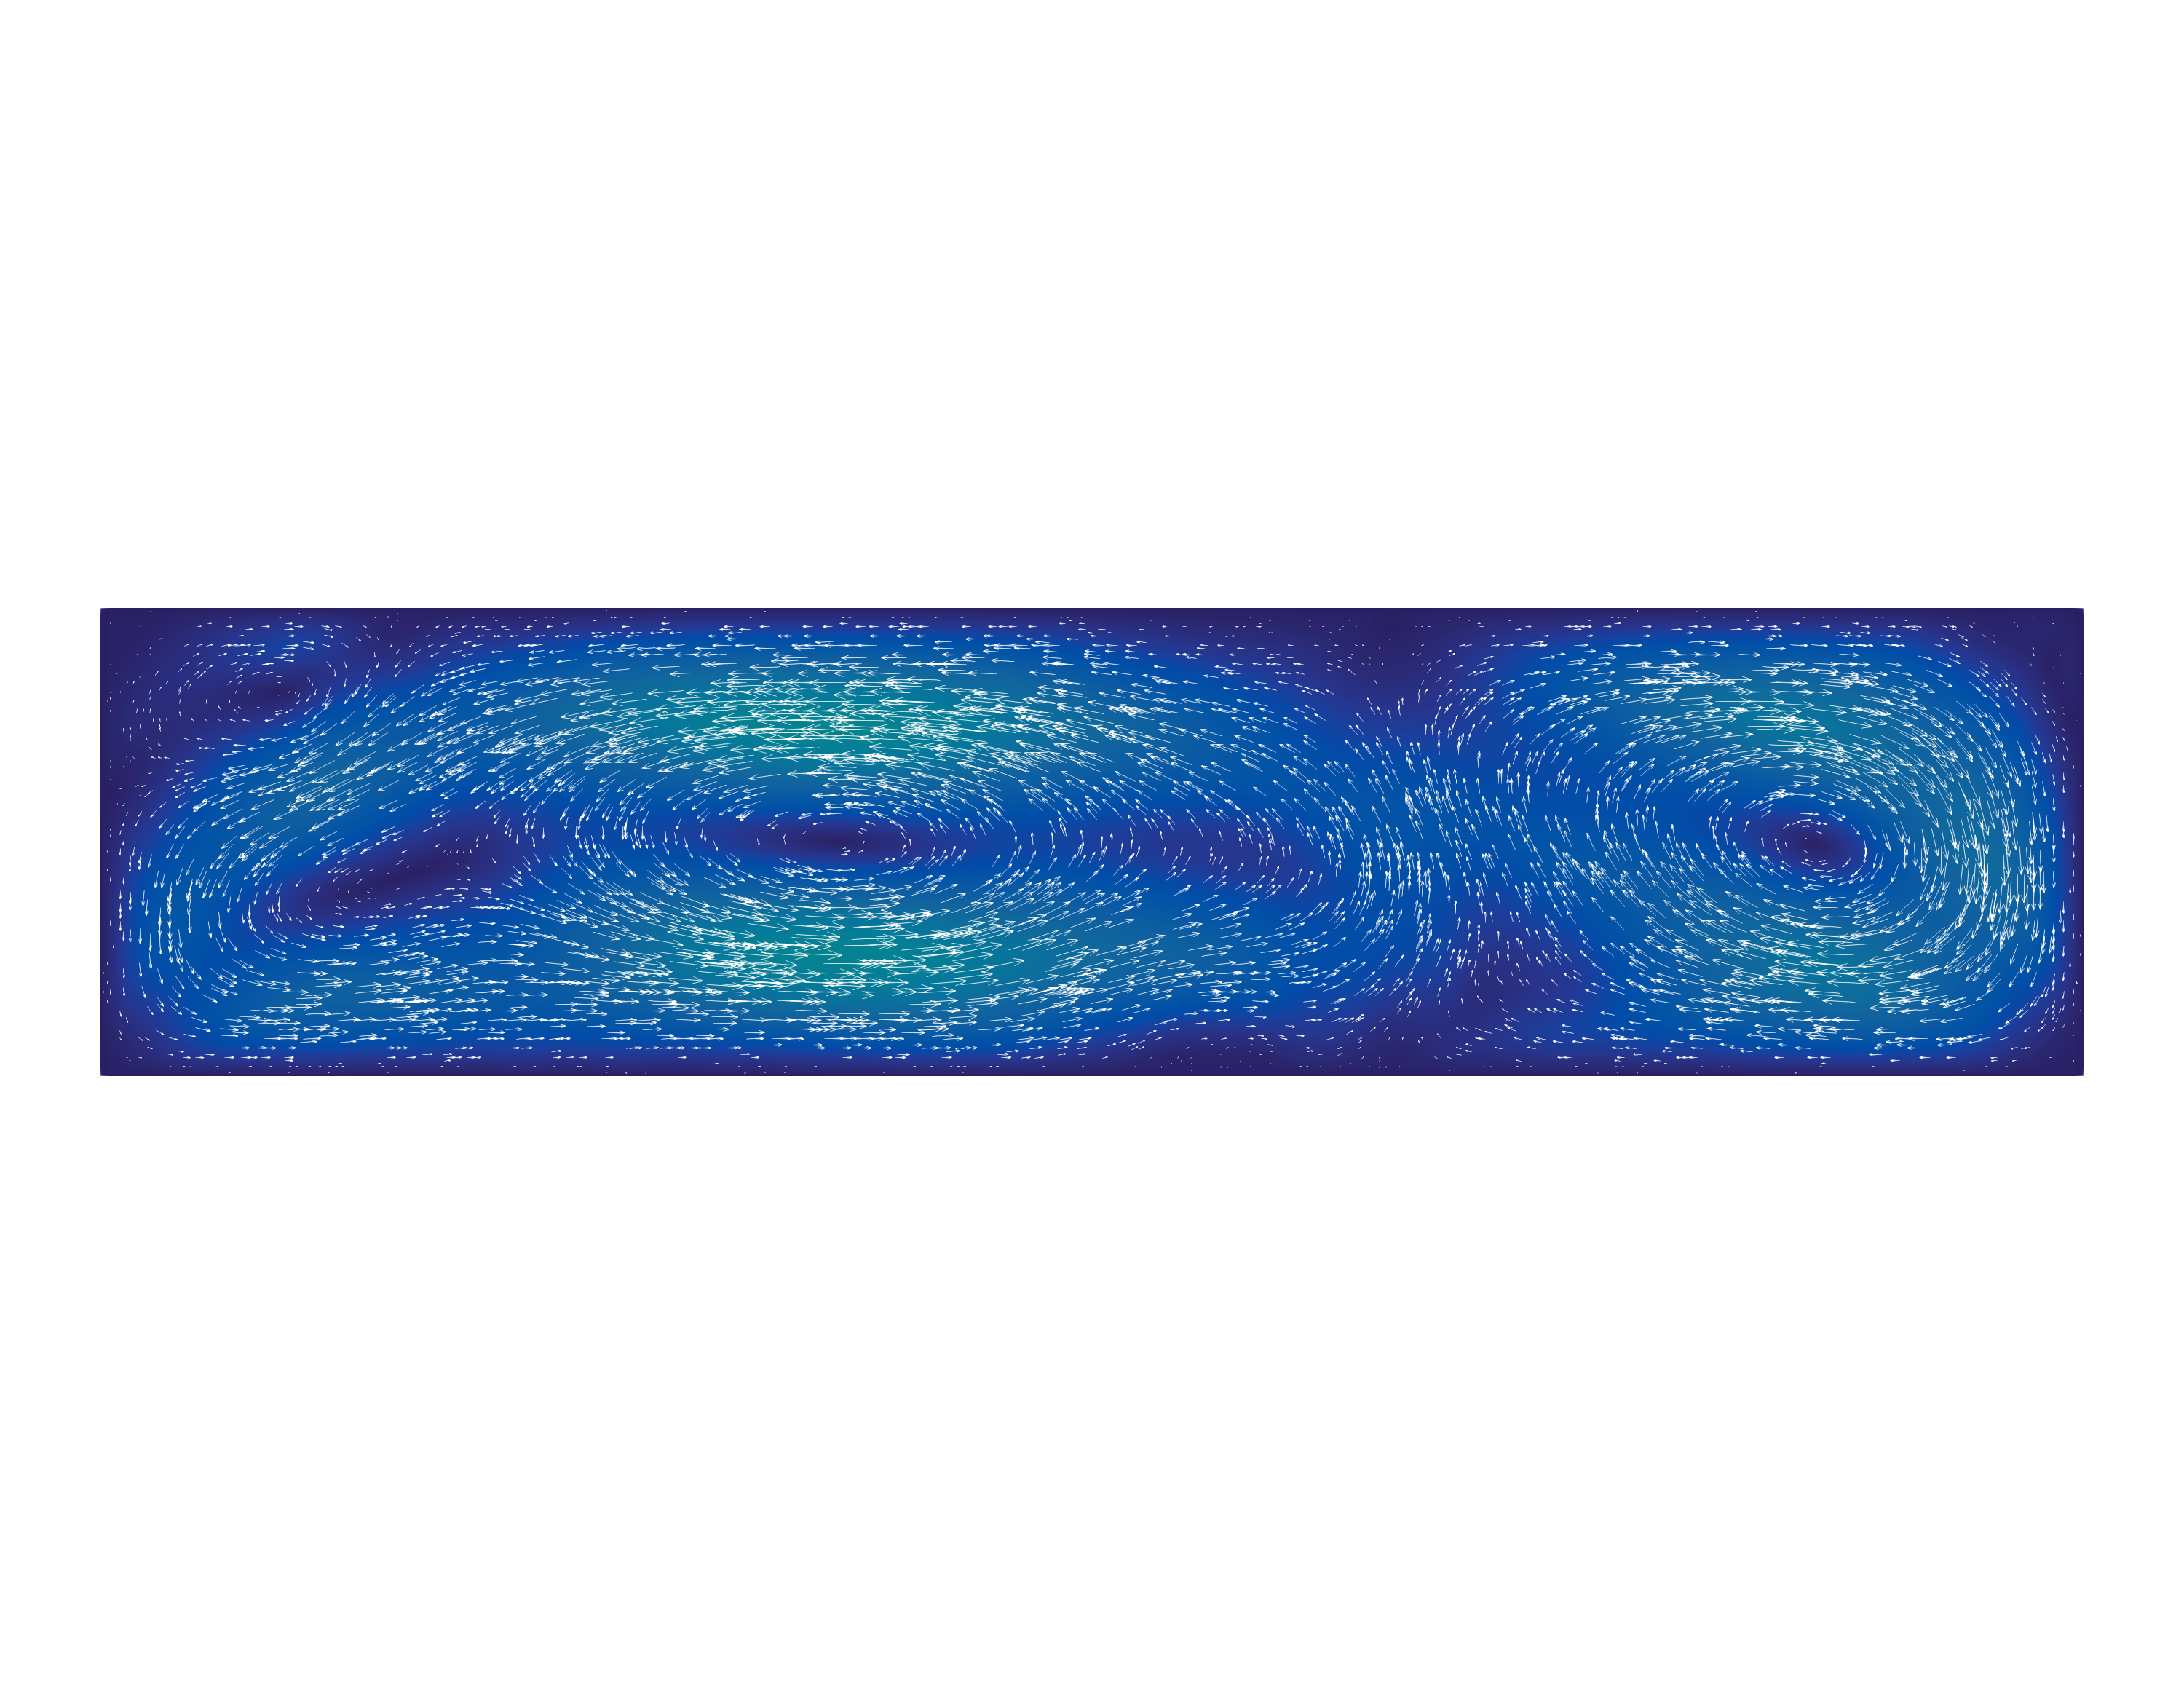
\includegraphics[width=0.9\textwidth]{../media/fourier/application/print/ab-0-1-velocity-harm.png}
        \caption{Anode $(1,1)$ désactivée}
        \label{fig:}
      \end{center}
    \end{subfigure}

    \begin{subfigure}[t]{\textwidth}
      \begin{center}
        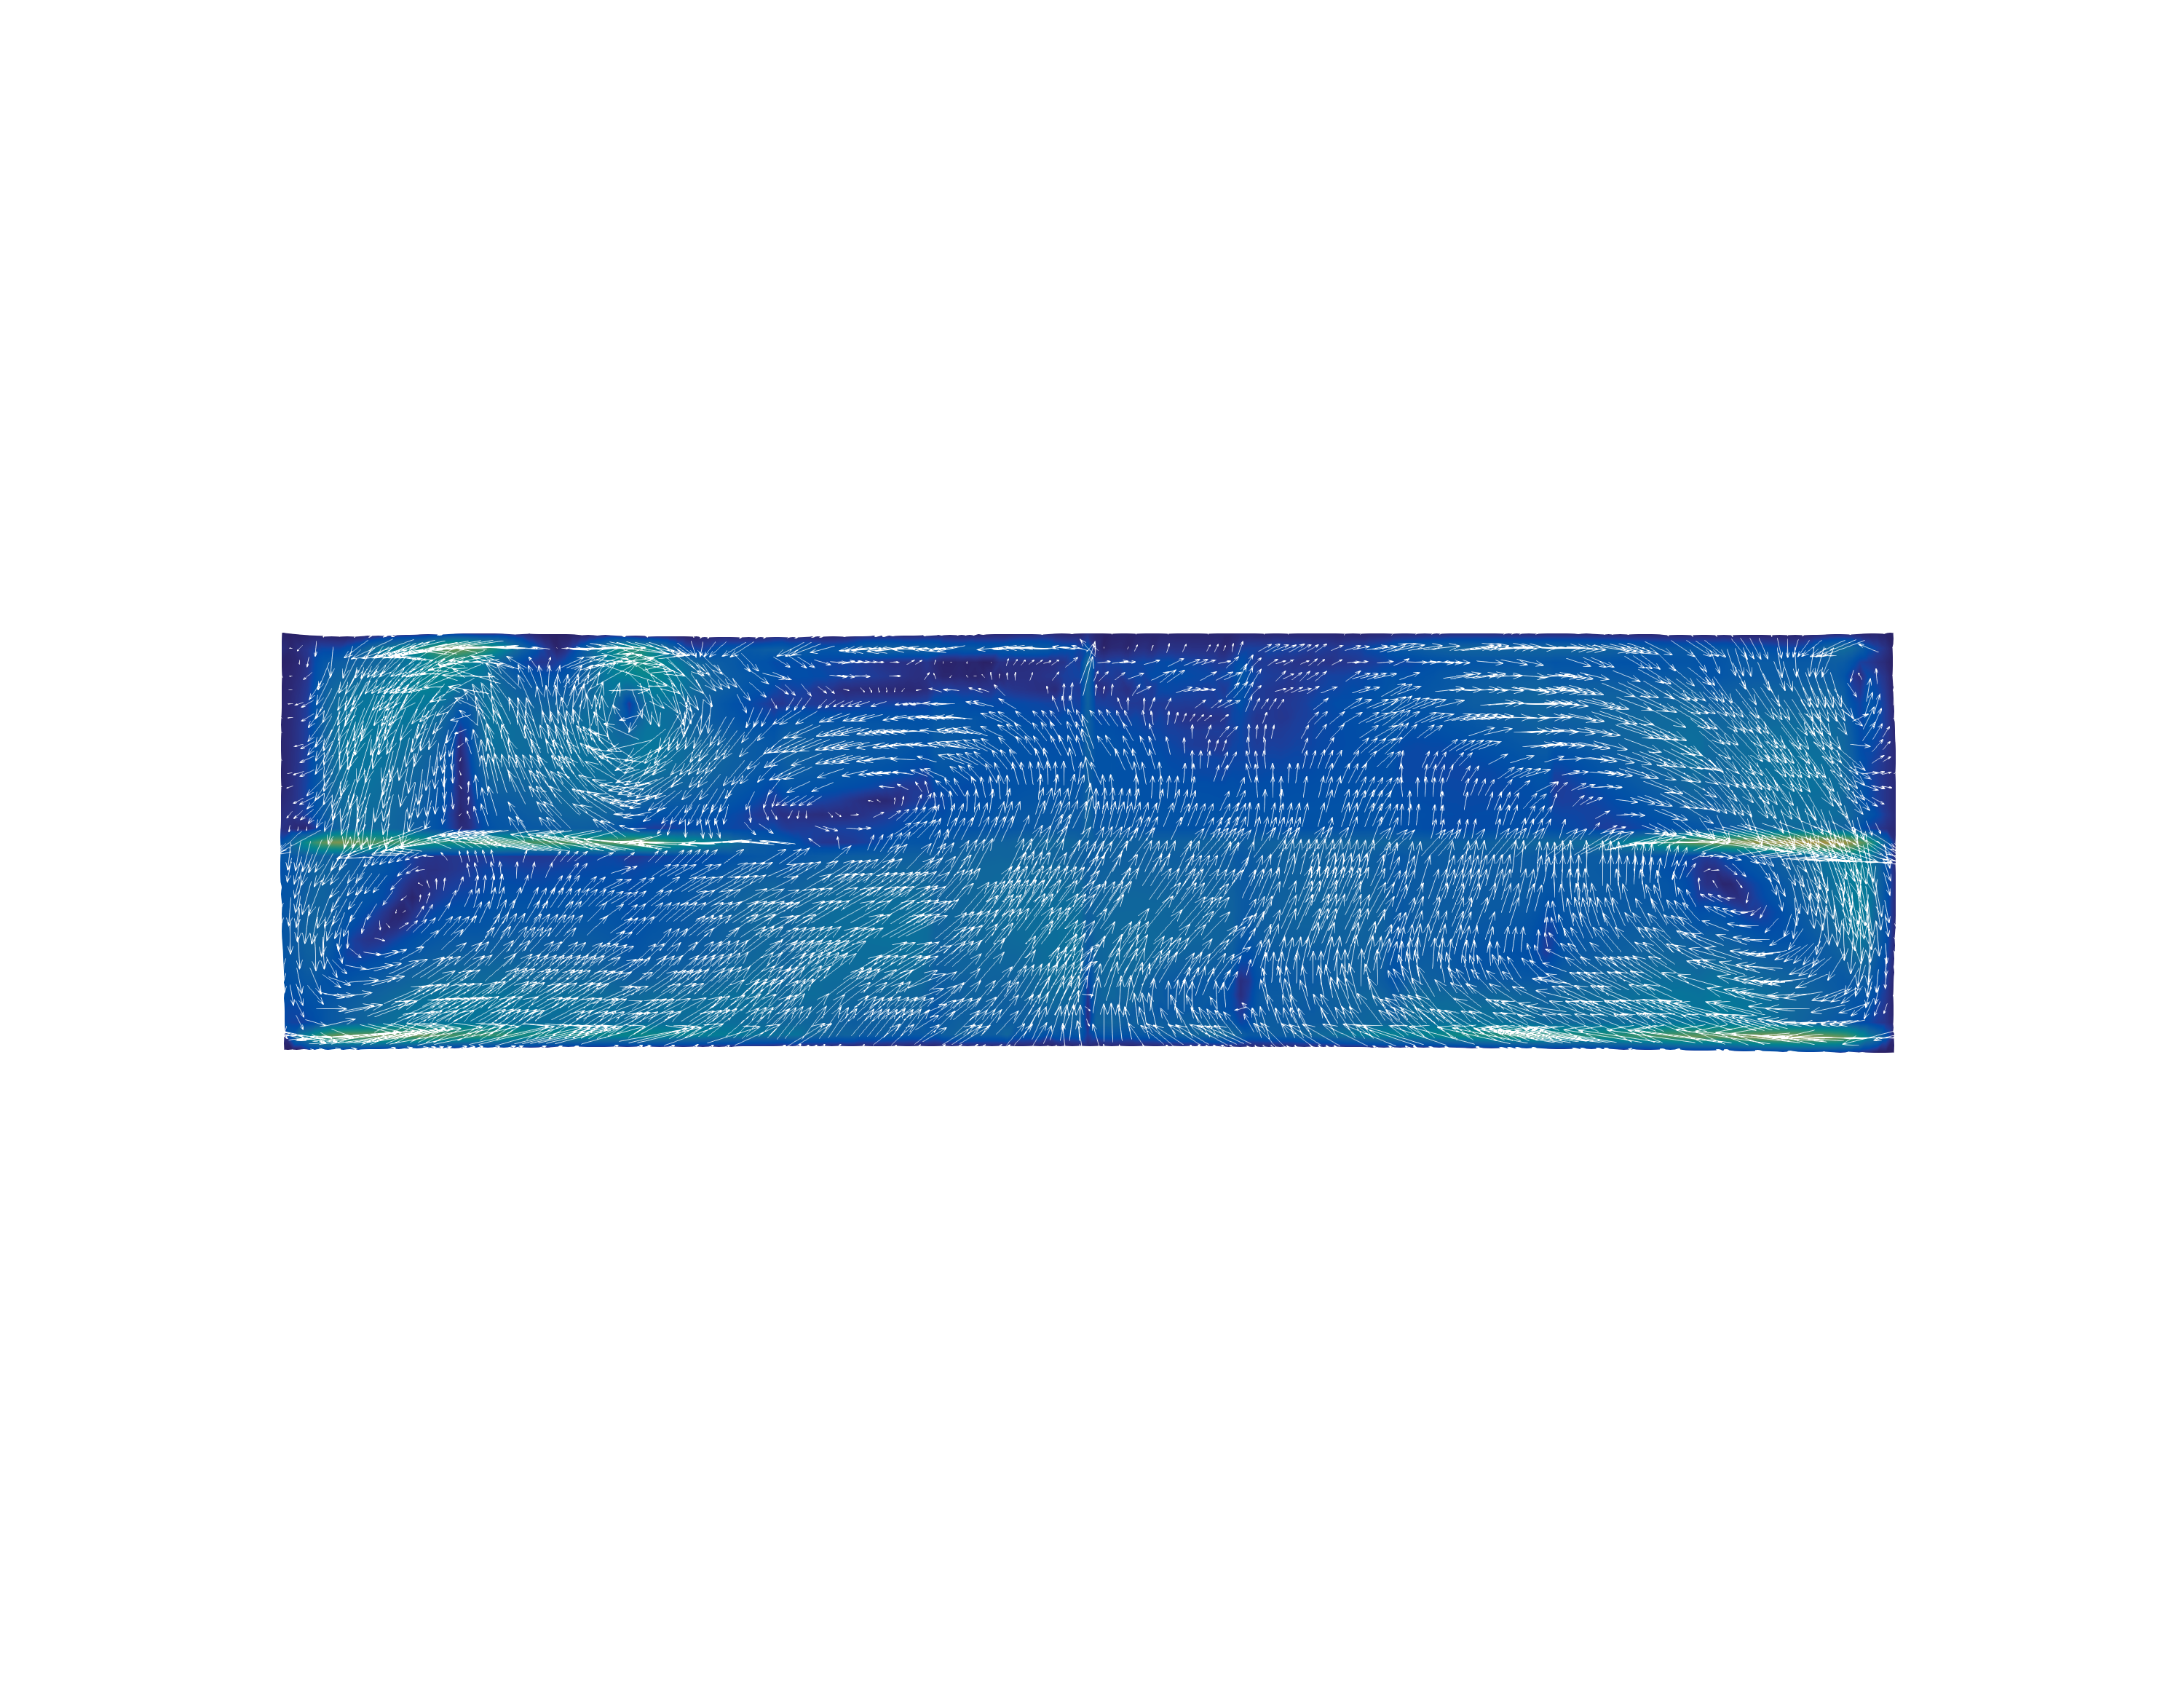
\includegraphics[width=0.9\textwidth]{../media/fourier/application/print/ab-0-2-velocity-acd.png}
        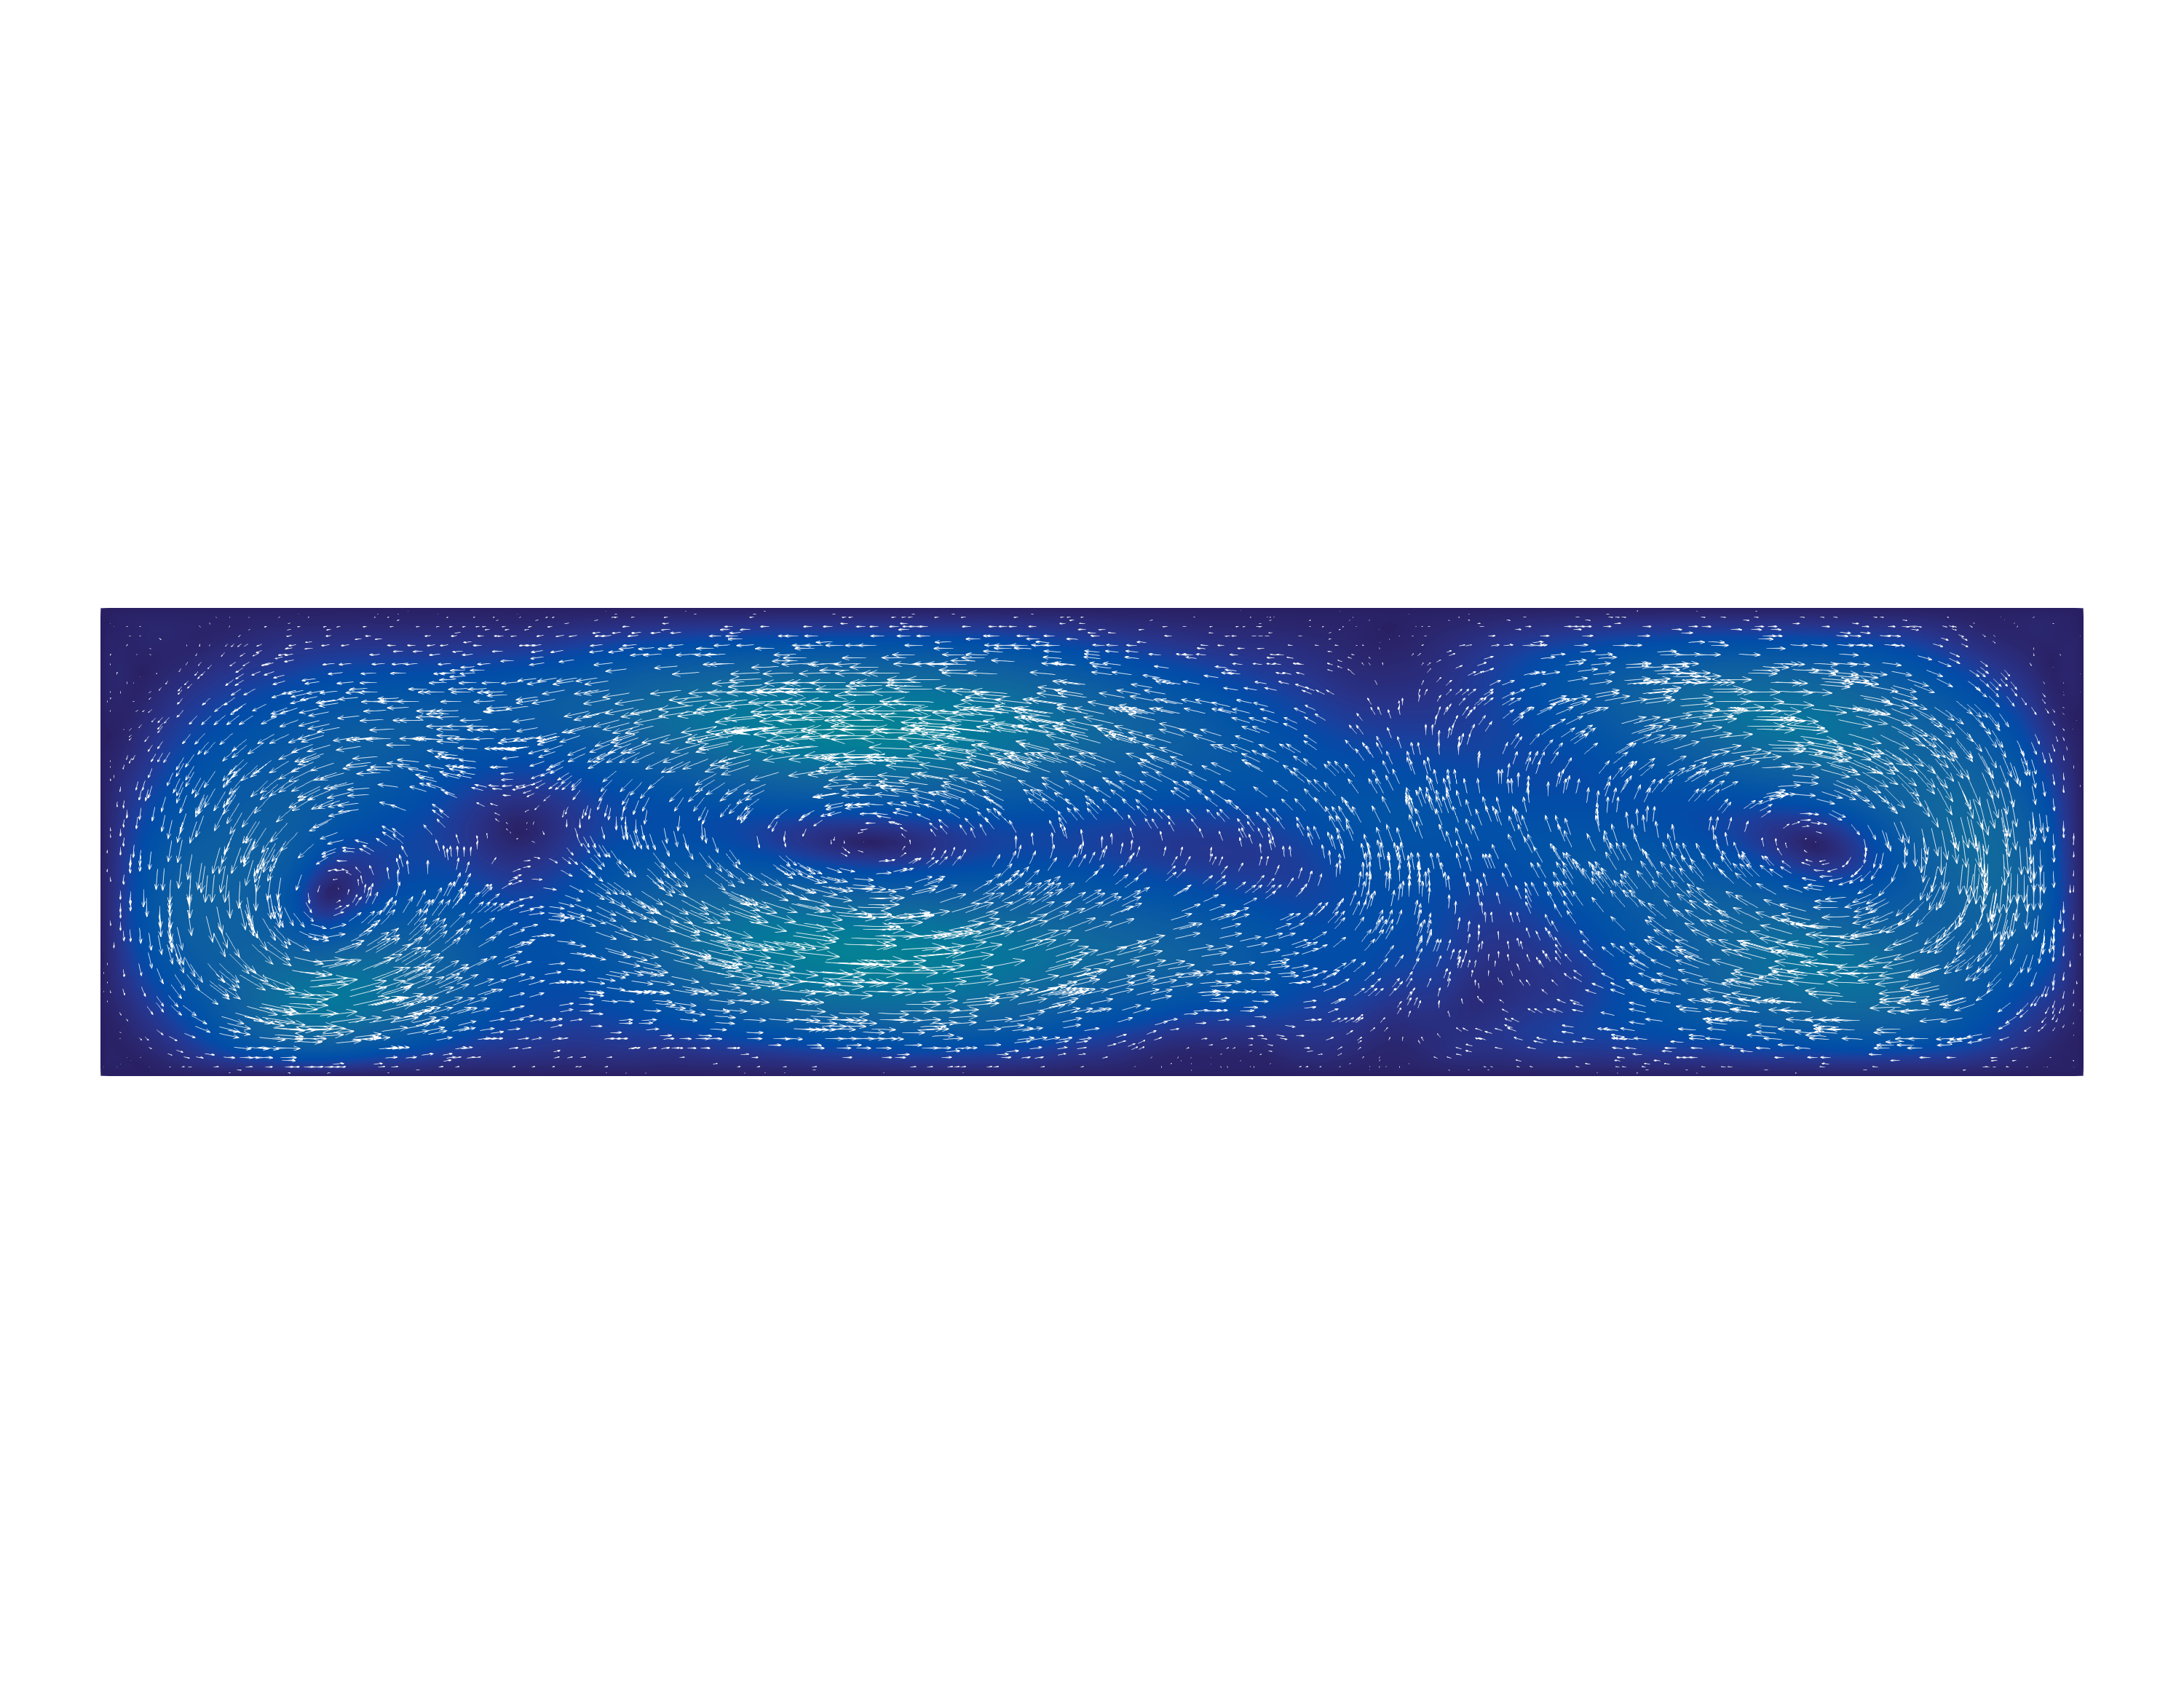
\includegraphics[width=0.9\textwidth]{../media/fourier/application/print/ab-0-2-velocity-harm.png}
        \caption{Anode $(1,2)$ désactivée}
        \label{fig:}
      \end{center}
    \end{subfigure}

    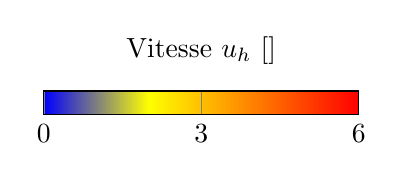
\begin{tikzpicture}
      \begin{axis}[
          colorbar,
          hide axis,
          scale only axis,
          height=0.10\textwidth,
          width=0.5\textwidth,
          colorbar horizontal,
          point meta min=0.0,
          point meta max=6.0,
          colorbar style={
            title=Vitesse $u_h$ [\si{\centi\meter\per\second}],
            width=4cm,
            height=0.3cm,
            xtick={0.0, 3.0, 6.0},
            at={(0.3\textwidth,0.4cm)},
            anchor=north
          }
        ]
        \addplot [] coordinates {(0,0)};
        \node (myfirstpic) at (0,0) {};
      \end{axis}
    \end{tikzpicture}

    \caption{Vitesse d'écoulement $u_h^\mathrm{S3D}$ dans l'ACD (haut)
      et $u_h^\mathrm{SF}$ sur une surface $x_3 = \thickness / 2$ à
      mi-hauteur dans le domaine $\Omega$ (bas).}

    \label{fig:harmonic-velocity-comp-a}
  \end{center}
\end{figure}


\begin{figure}[h!]
  \begin{center}
    \begin{subfigure}[t]{\textwidth}
      \begin{center}
        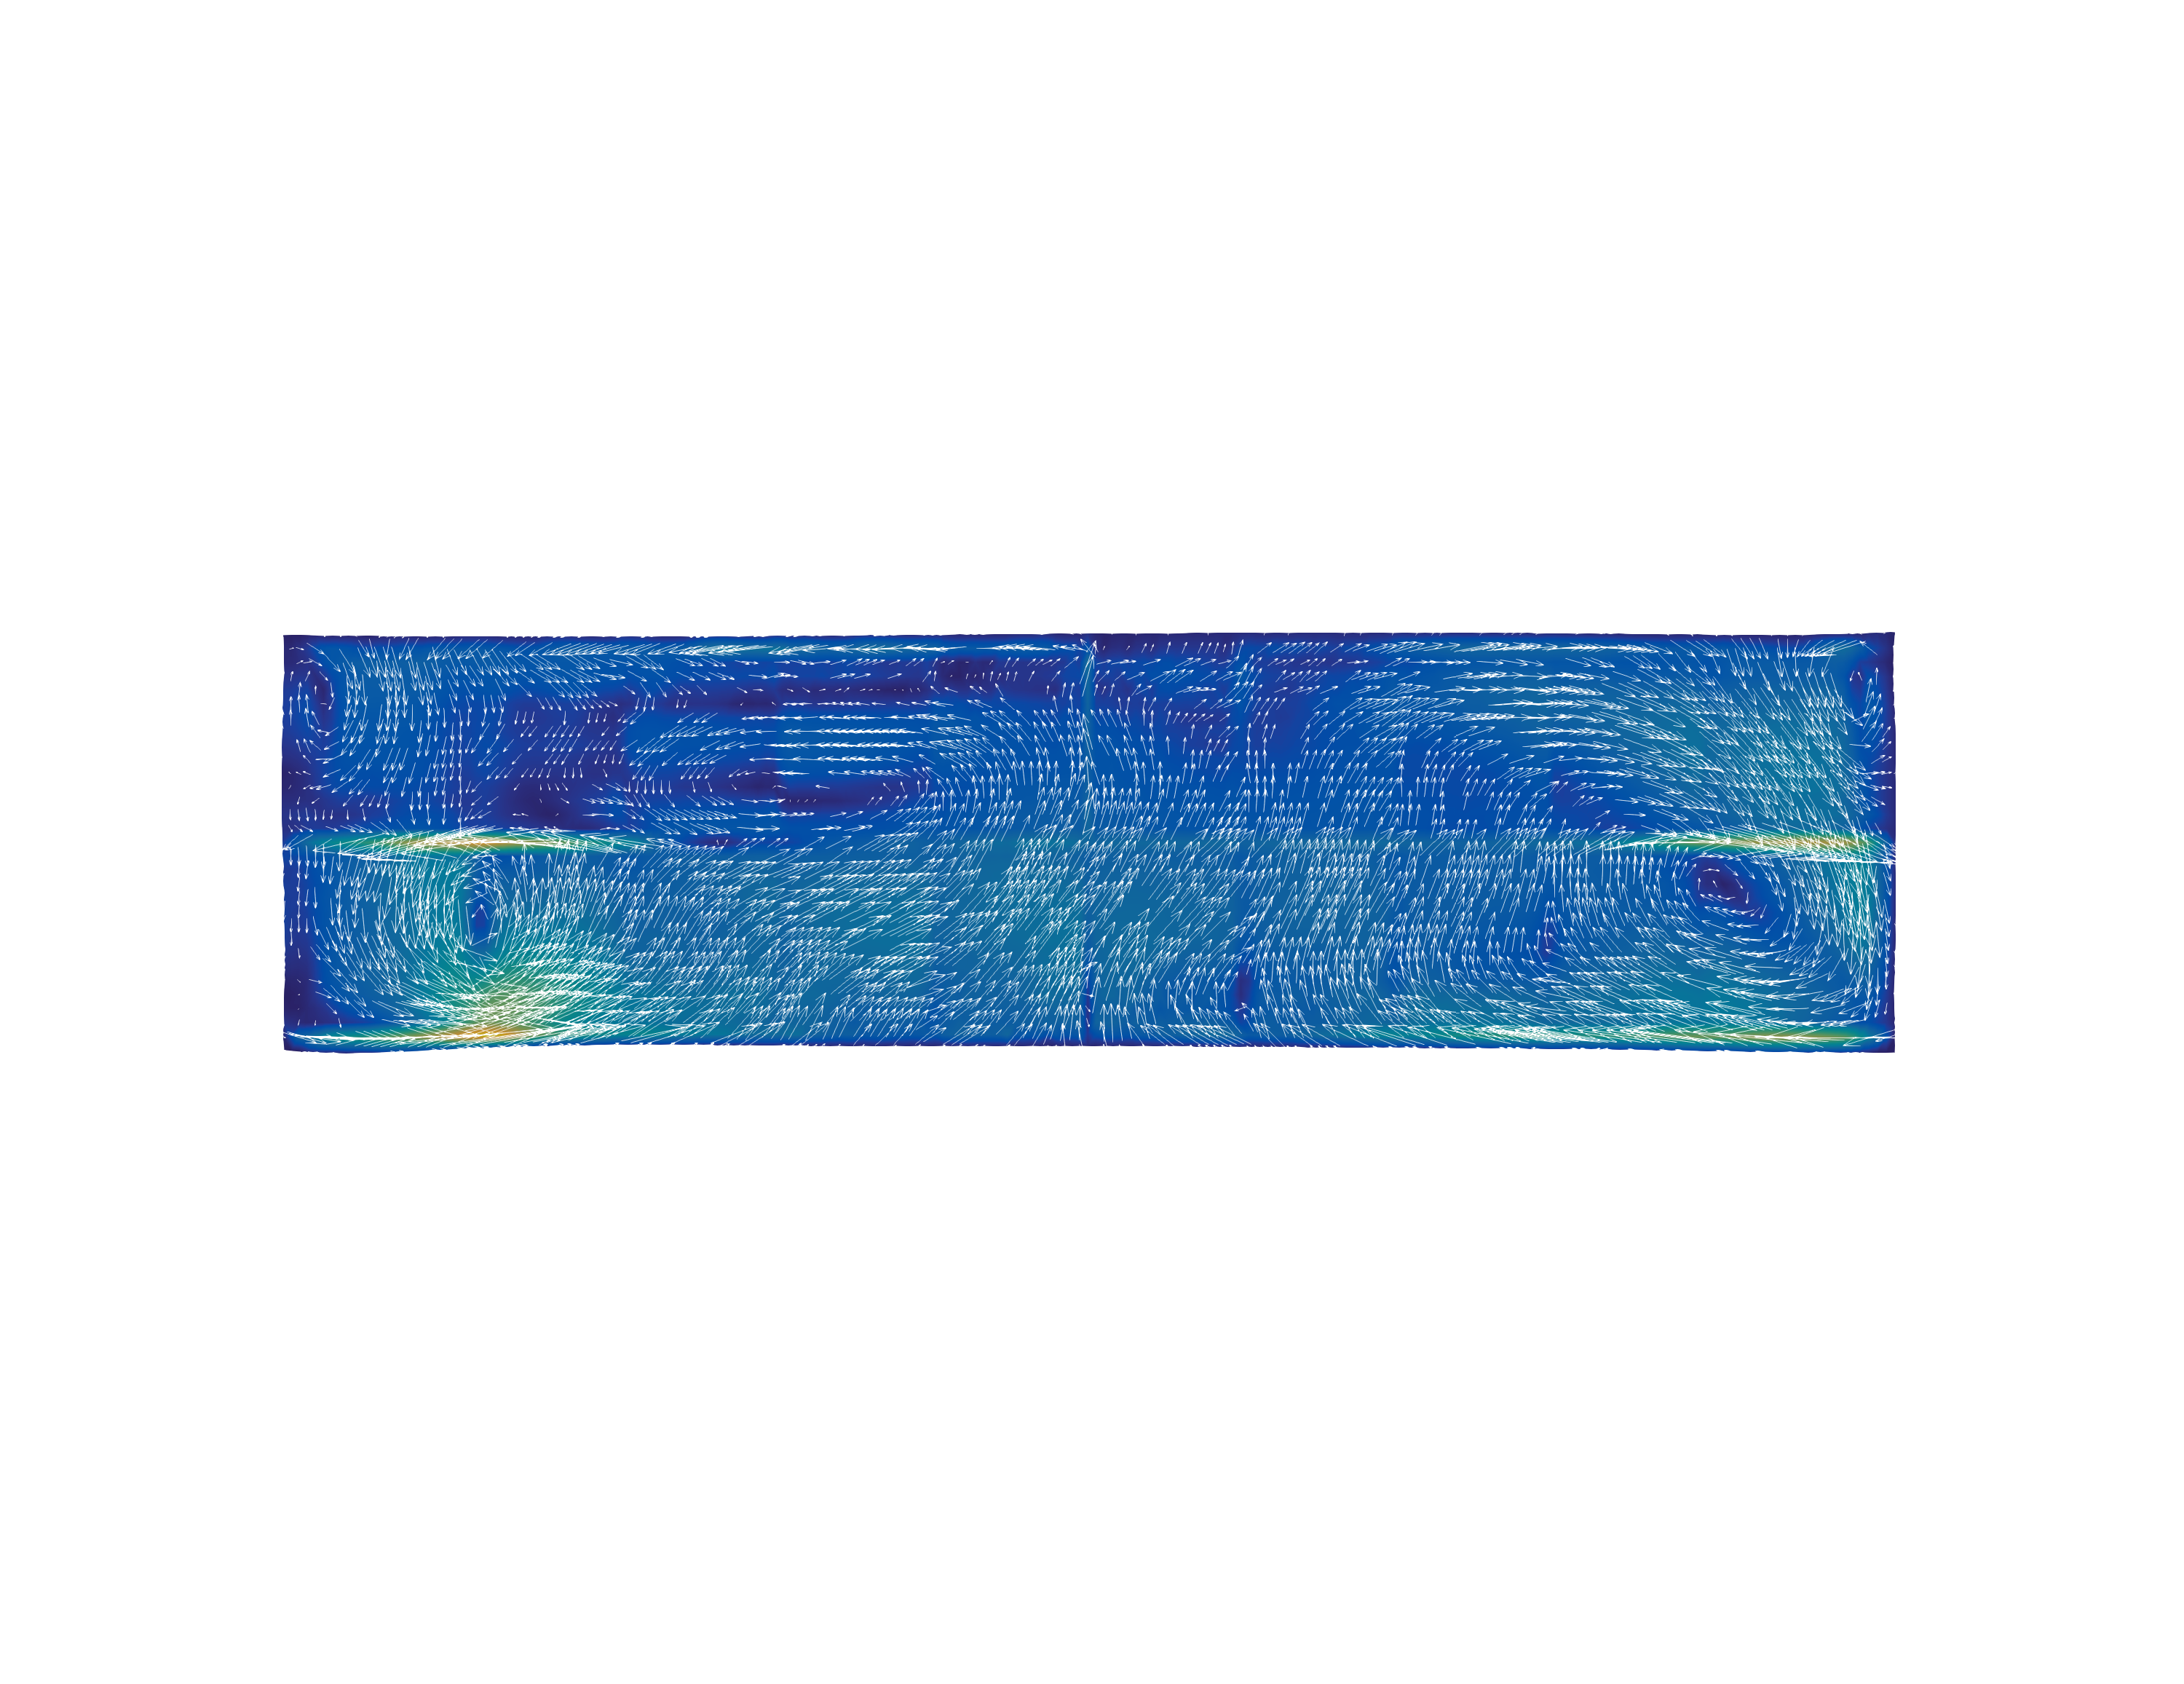
\includegraphics[width=0.9\textwidth]{../media/fourier/application/print/ab-1-1-velocity-acd.png}
        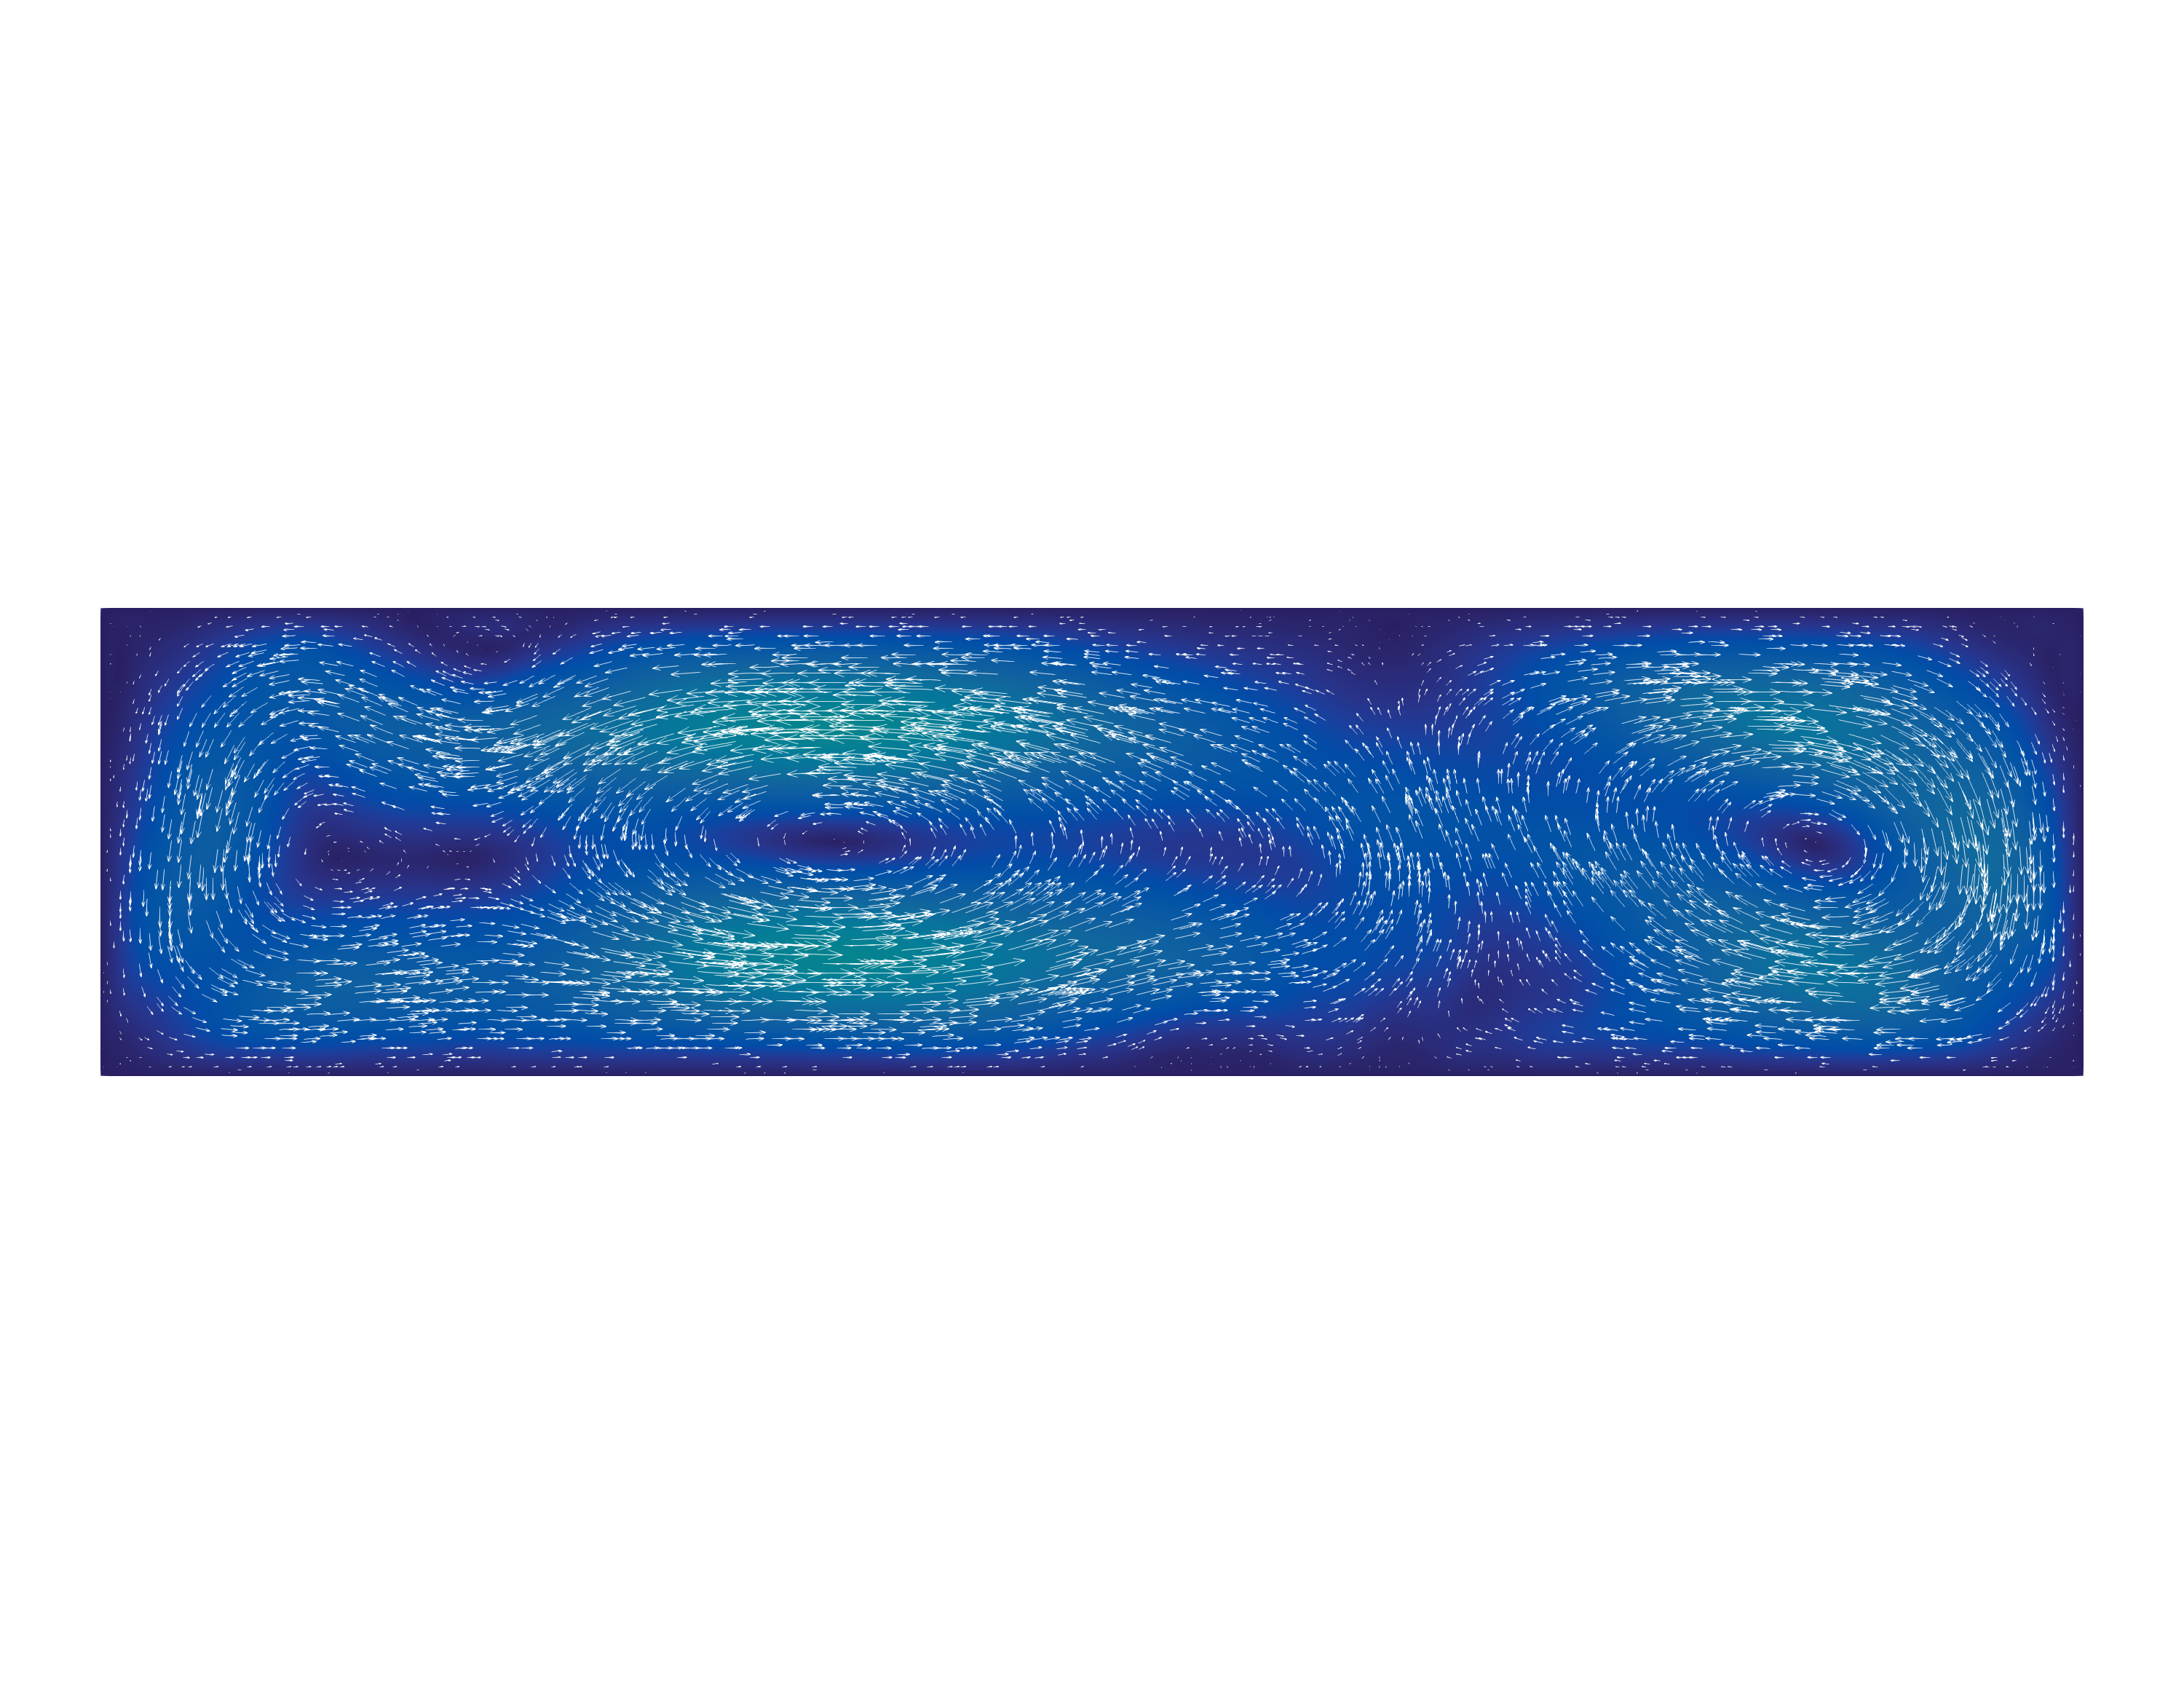
\includegraphics[width=0.9\textwidth]{../media/fourier/application/print/ab-1-1-velocity-harm.png}
        \caption{Anode $(2,1)$ désactivée}
        \label{fig:}
      \end{center}
    \end{subfigure}

    \begin{subfigure}[t]{\textwidth}
      \begin{center}
        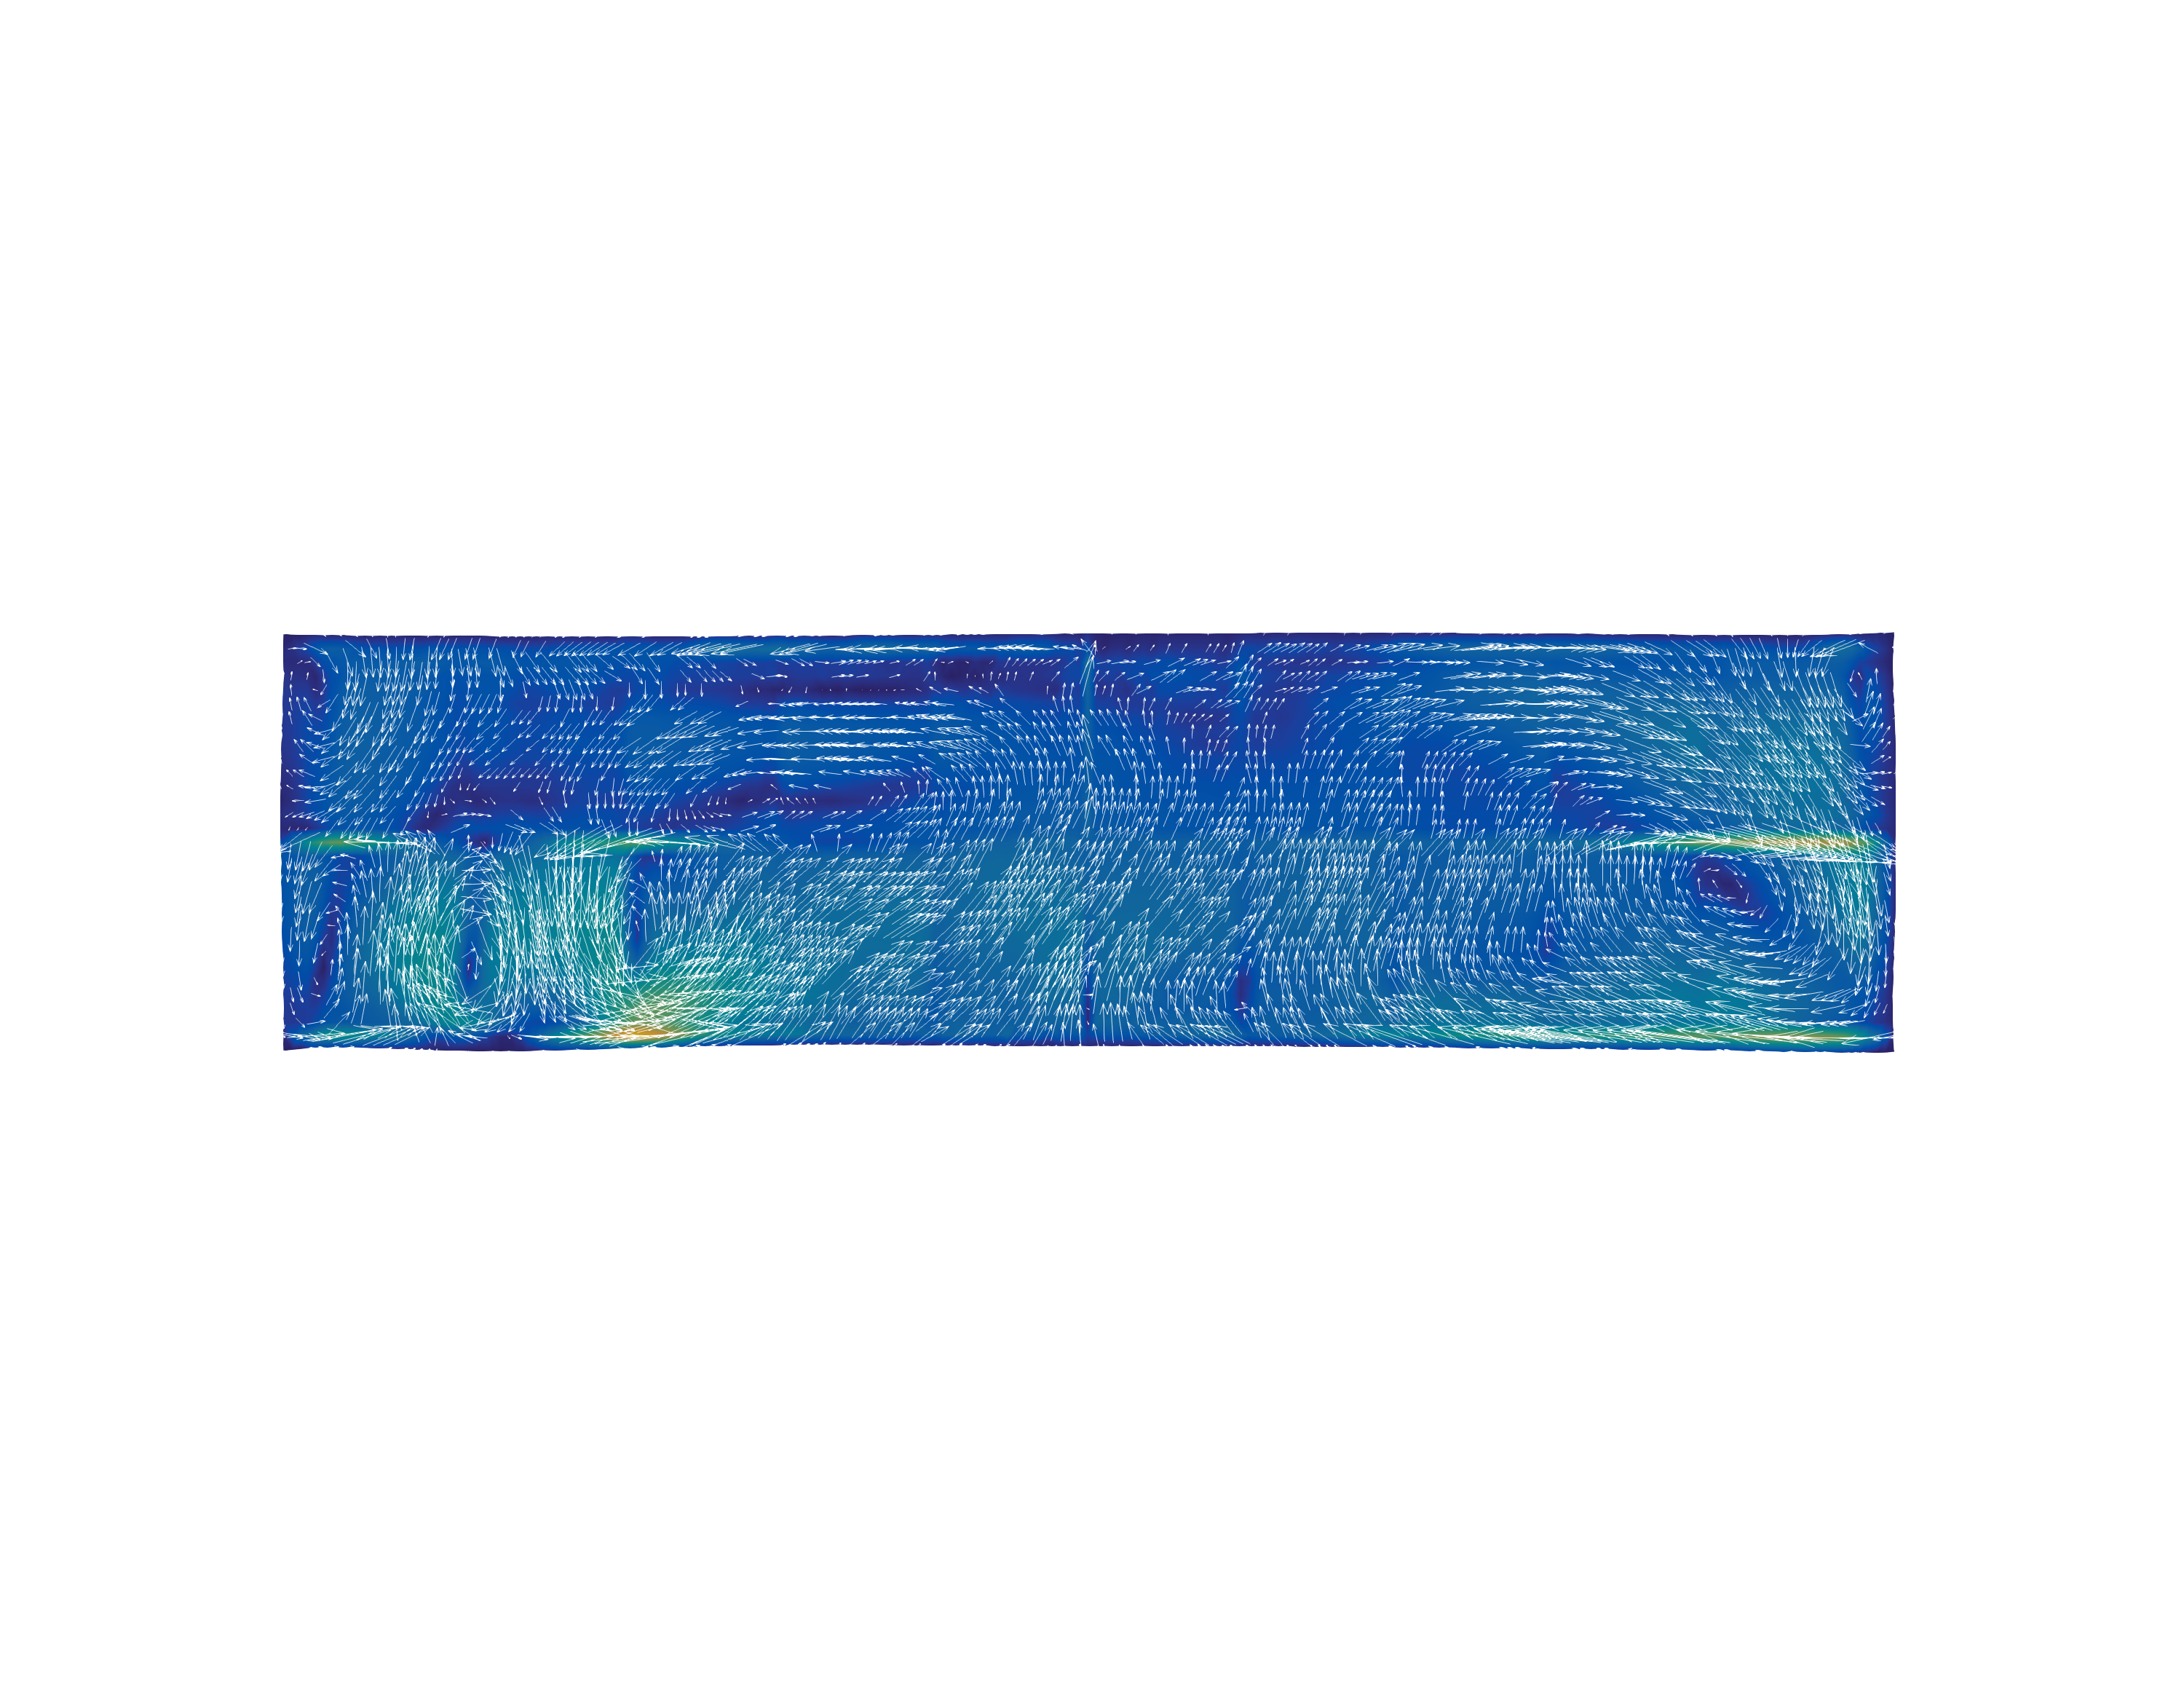
\includegraphics[width=0.9\textwidth]{../media/fourier/application/print/ab-1-2-velocity-acd.png}
        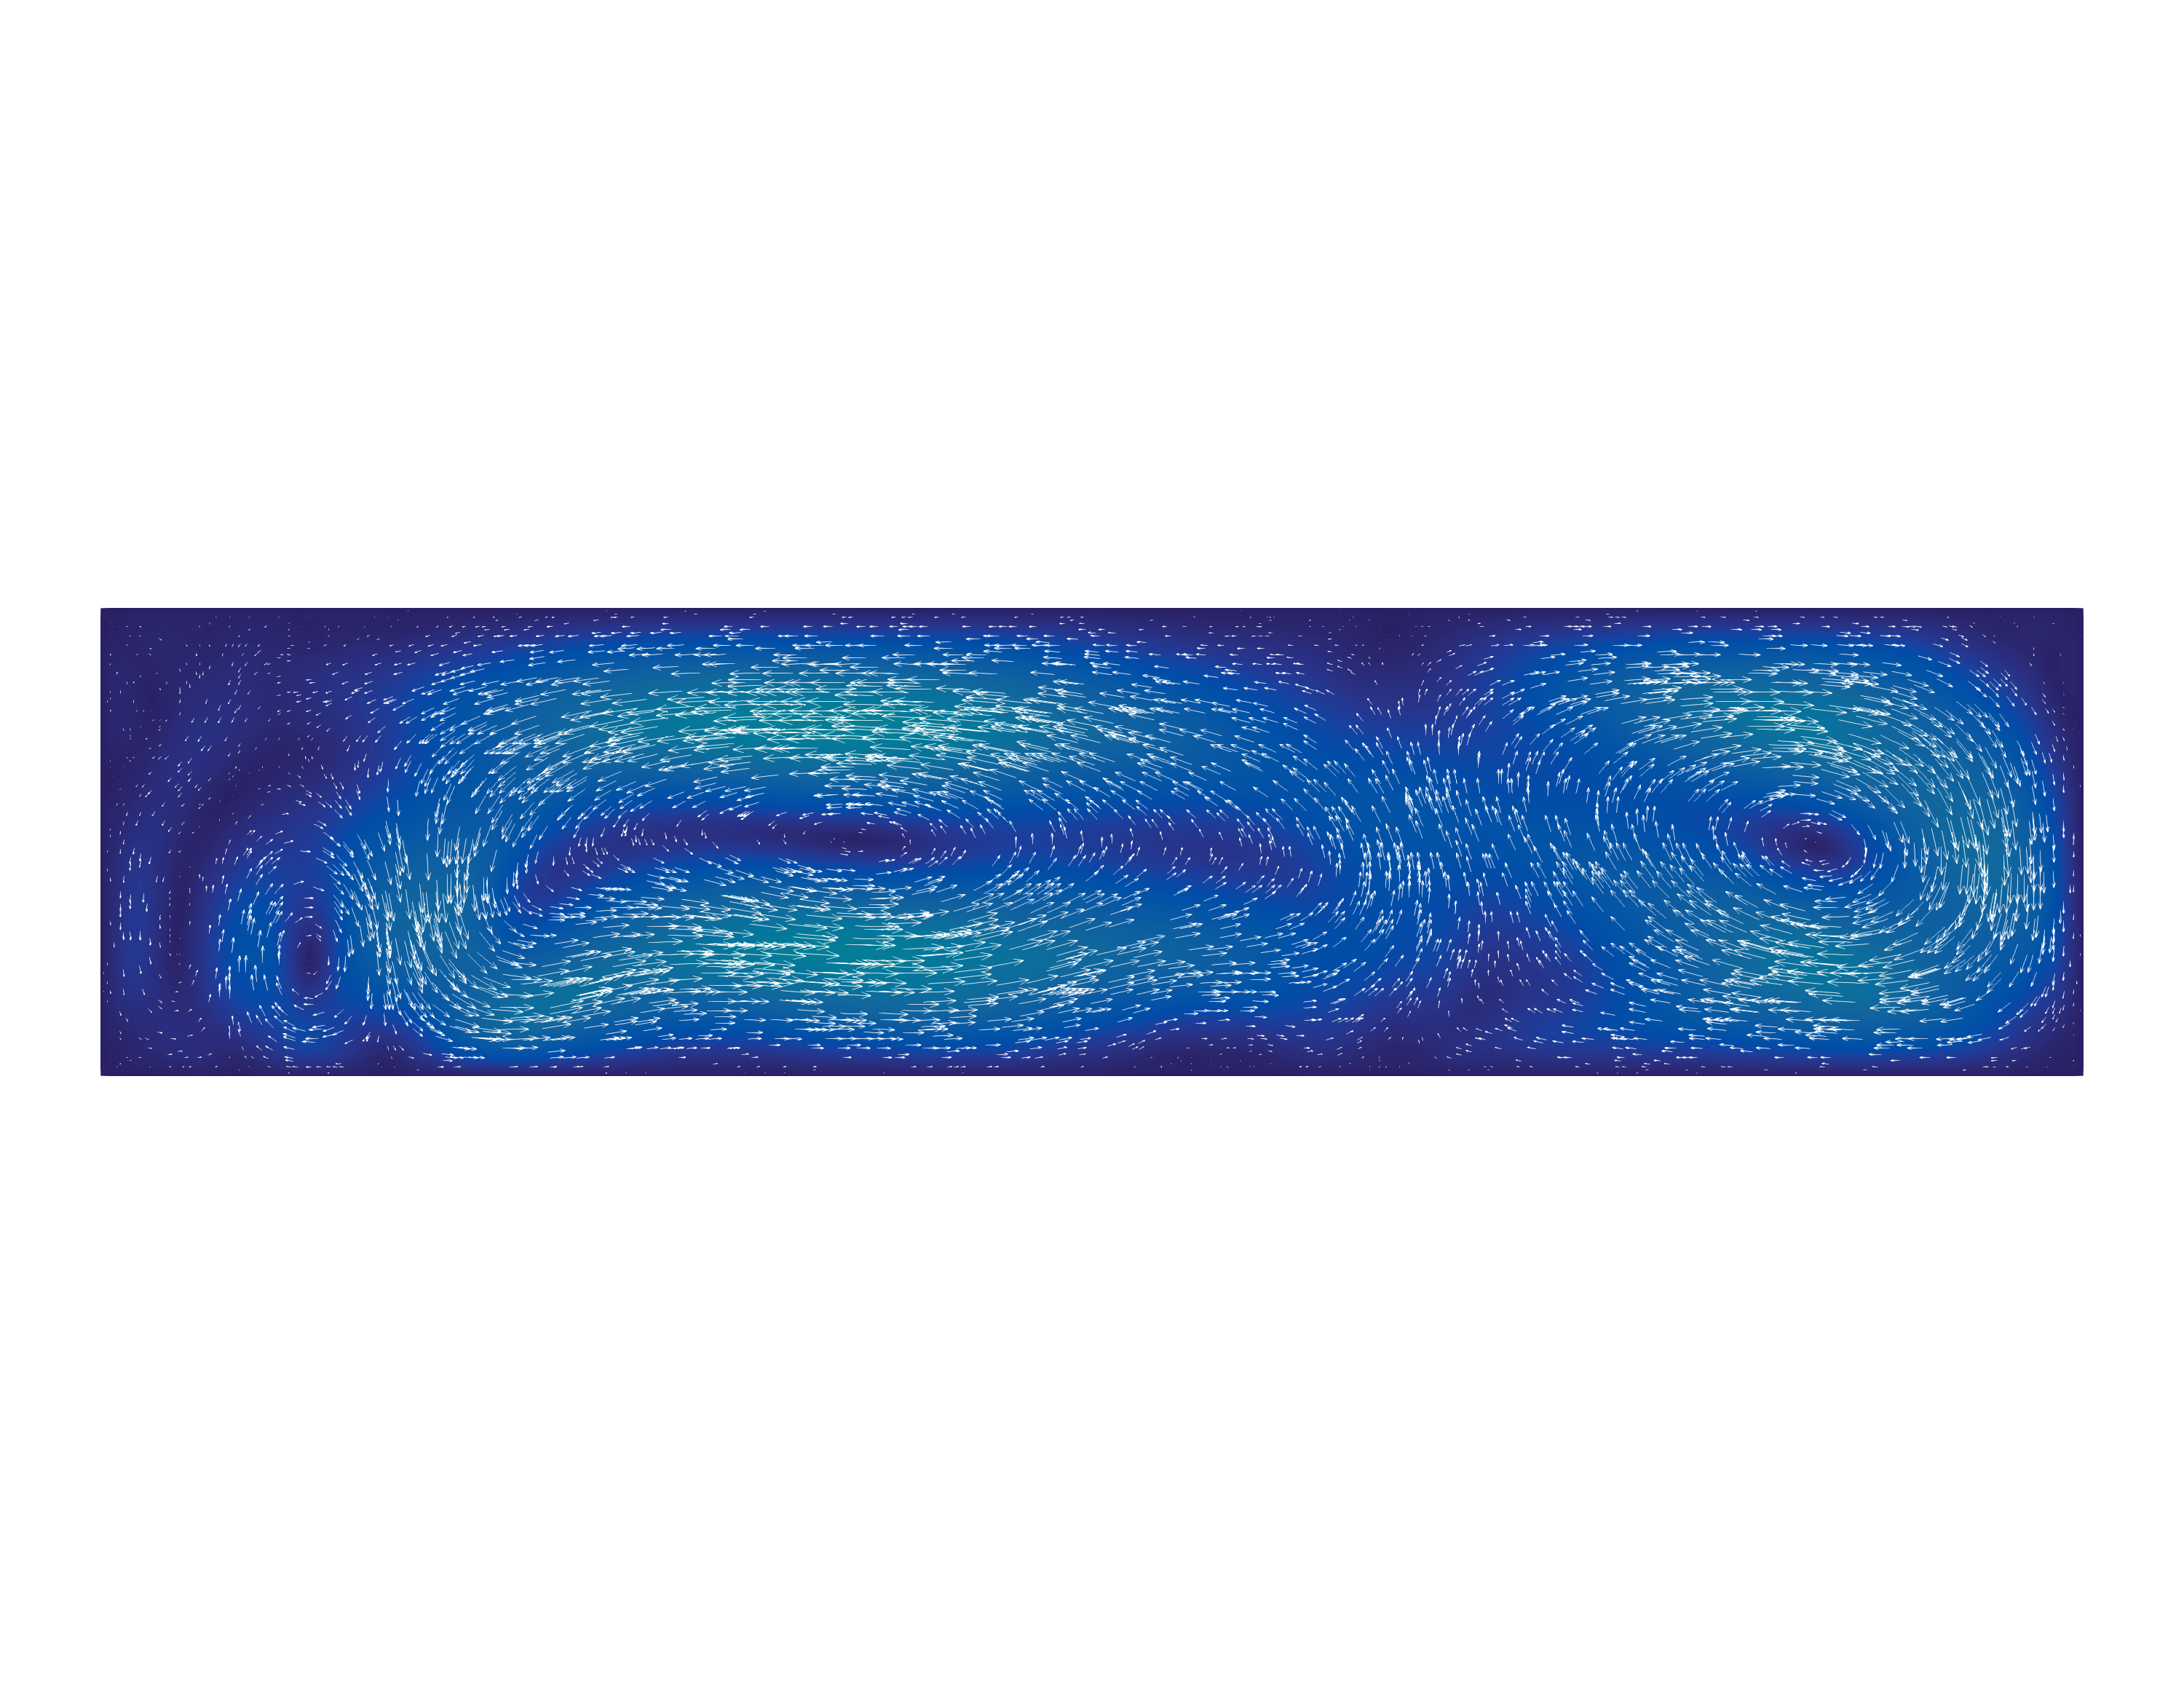
\includegraphics[width=0.9\textwidth]{../media/fourier/application/print/ab-1-2-velocity-harm.png}
        \caption{Anode $(2,2)$ désactivée}
        \label{fig:}
      \end{center}
    \end{subfigure}

    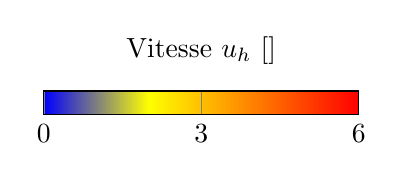
\begin{tikzpicture}
      \begin{axis}[
          colorbar,
          hide axis,
          scale only axis,
          height=0.10\textwidth,
          width=0.5\textwidth,
          colorbar horizontal,
          point meta min=0.0,
          point meta max=6.0,
          colorbar style={
            title=Vitesse $u_h$ [\si{\centi\meter\per\second}],
            width=4cm,
            height=0.3cm,
            xtick={0.0, 3.0, 6.0},
            at={(0.3\textwidth,0.4cm)},
            anchor=north
          }
        ]
        \addplot [] coordinates {(0,0)};
        \node (myfirstpic) at (0,0) {};
      \end{axis}
    \end{tikzpicture}

    \caption{Vitesse d'écoulement $u_h^\mathrm{S3D}$ dans l'ACD (haut)
      et $u_h^\mathrm{SF}$ sur une surface $x_3 = \thickness / 2$ à
      mi-hauteur dans le domaine $\Omega$ (bas).}

    \label{fig:harmonic-velocity-comp-b}
  \end{center}
\end{figure}

\begin{figure}[h!]
  \begin{center}
    \begin{subfigure}[t]{\textwidth}
      \begin{center}
        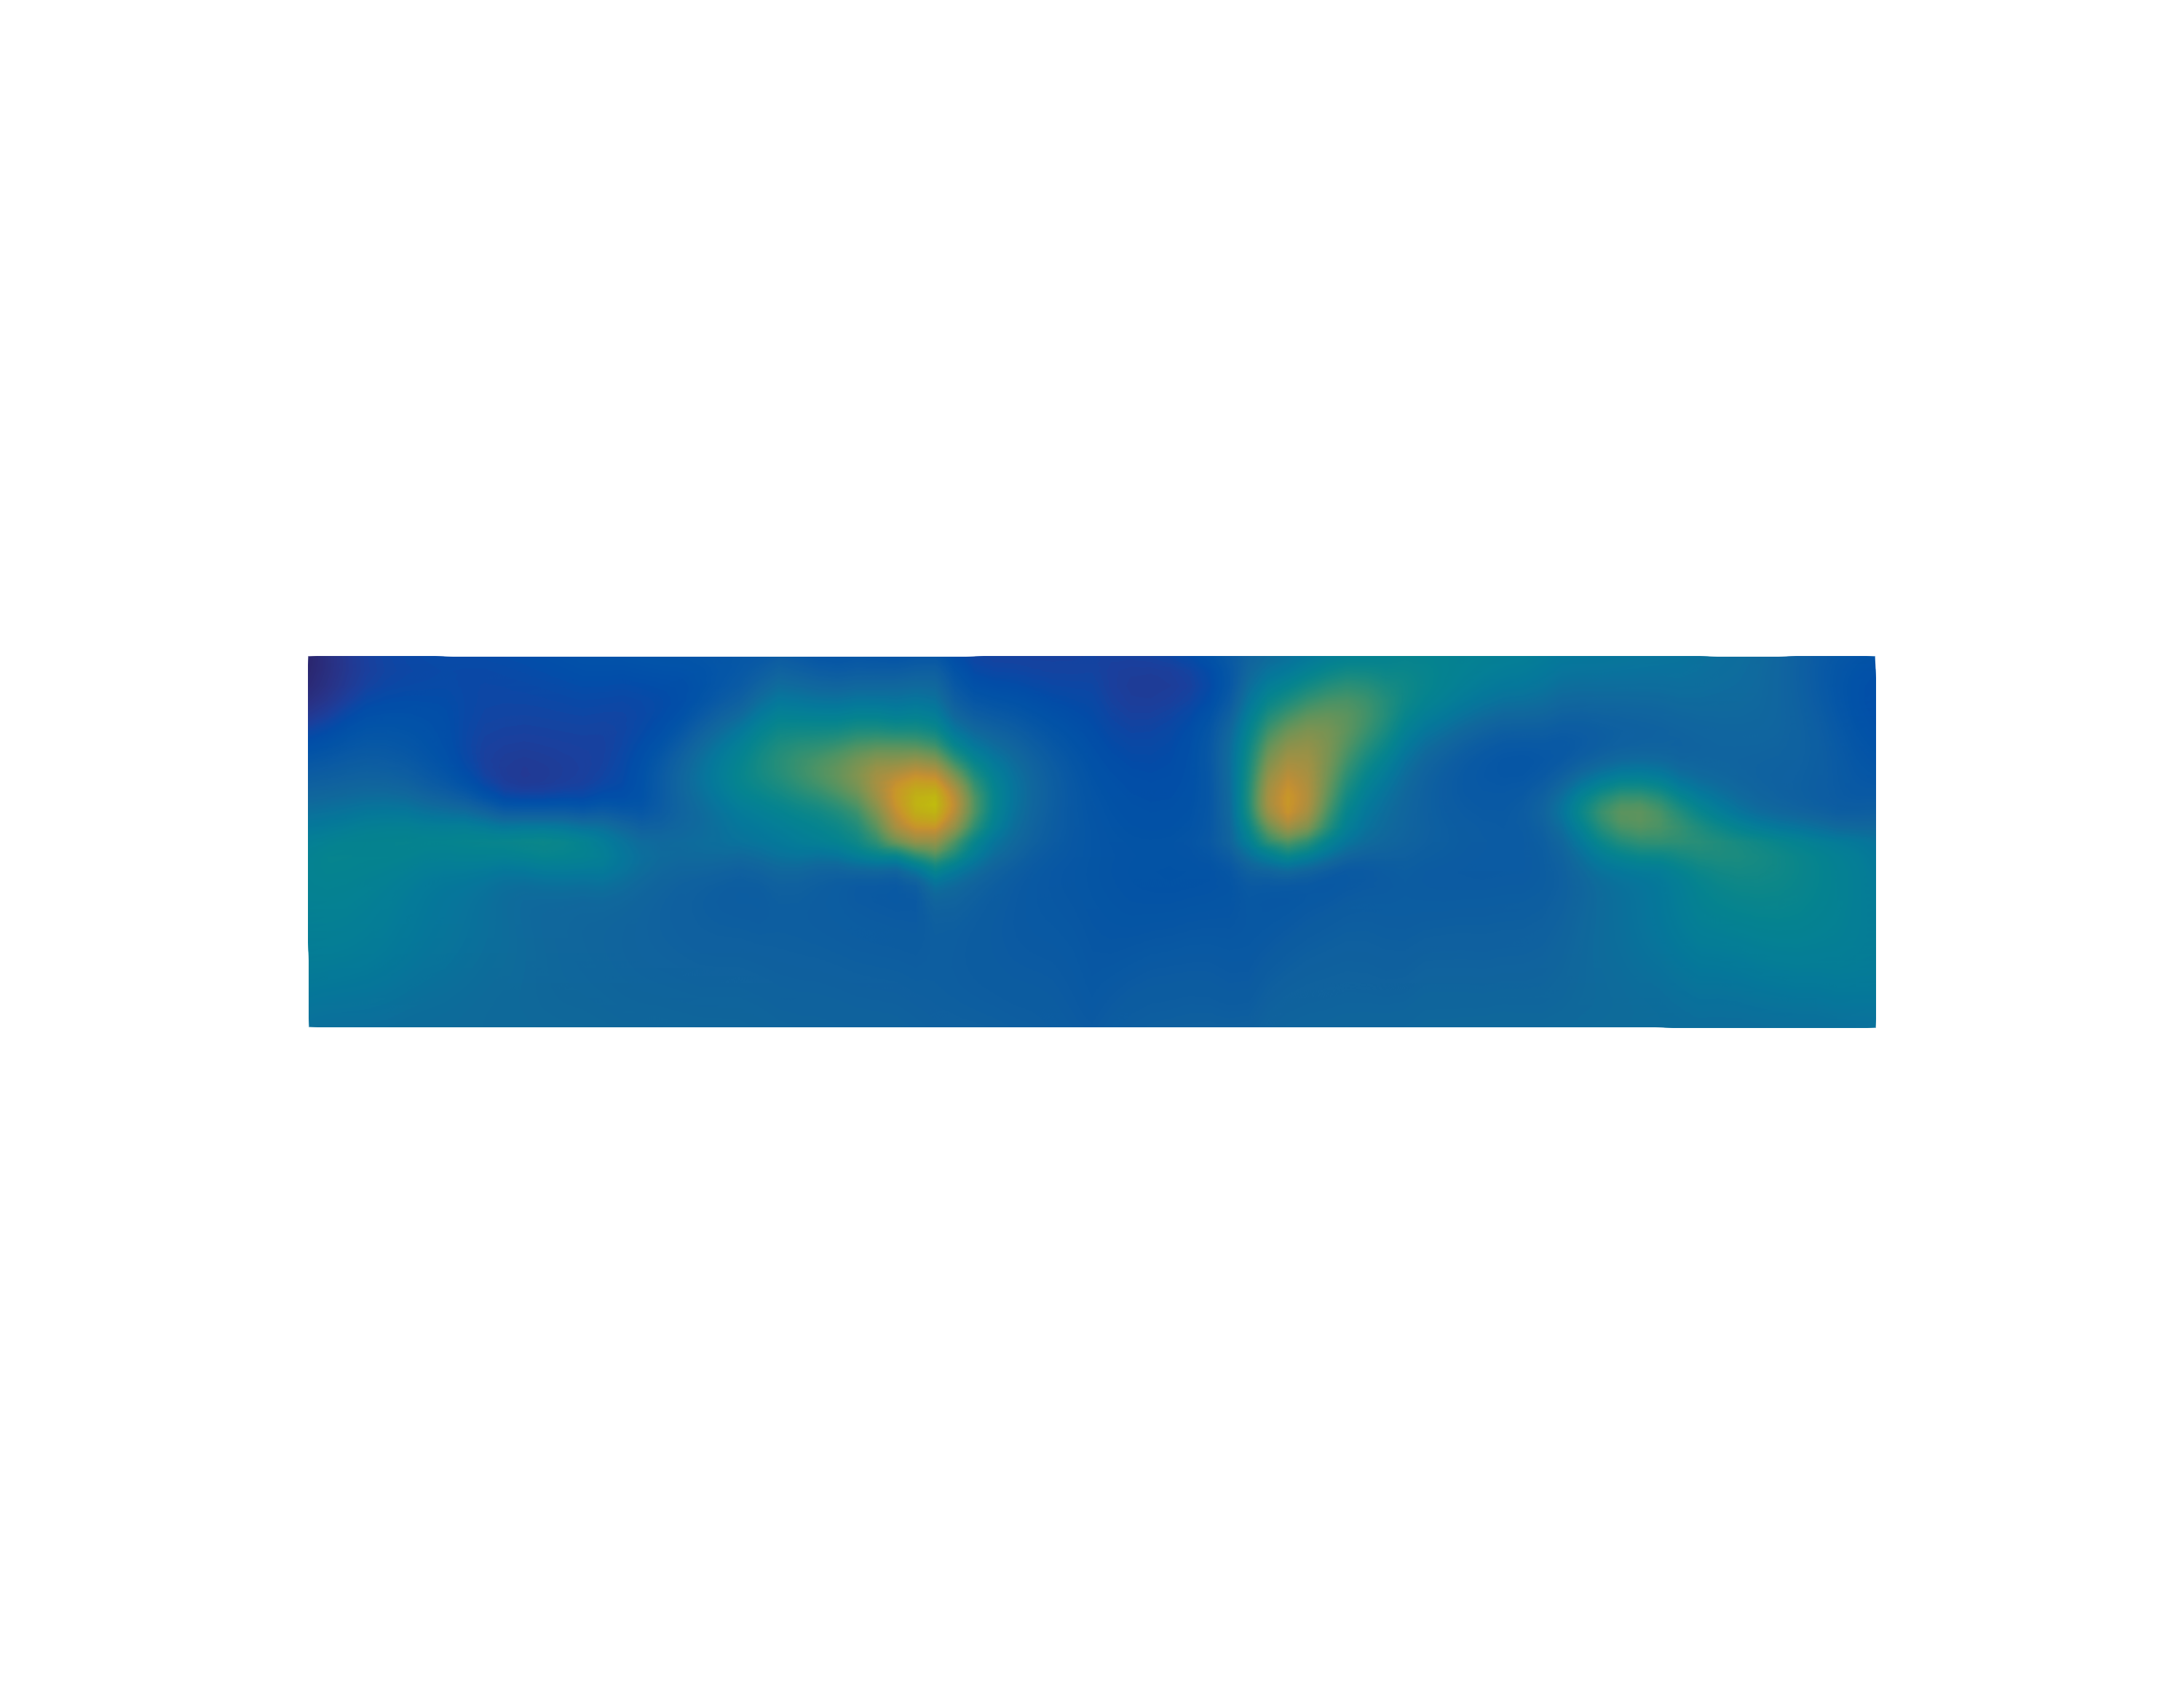
\includegraphics[width=0.99\textwidth]{../media/fourier/application/print/ab-0-1-concentration-acd.png}
        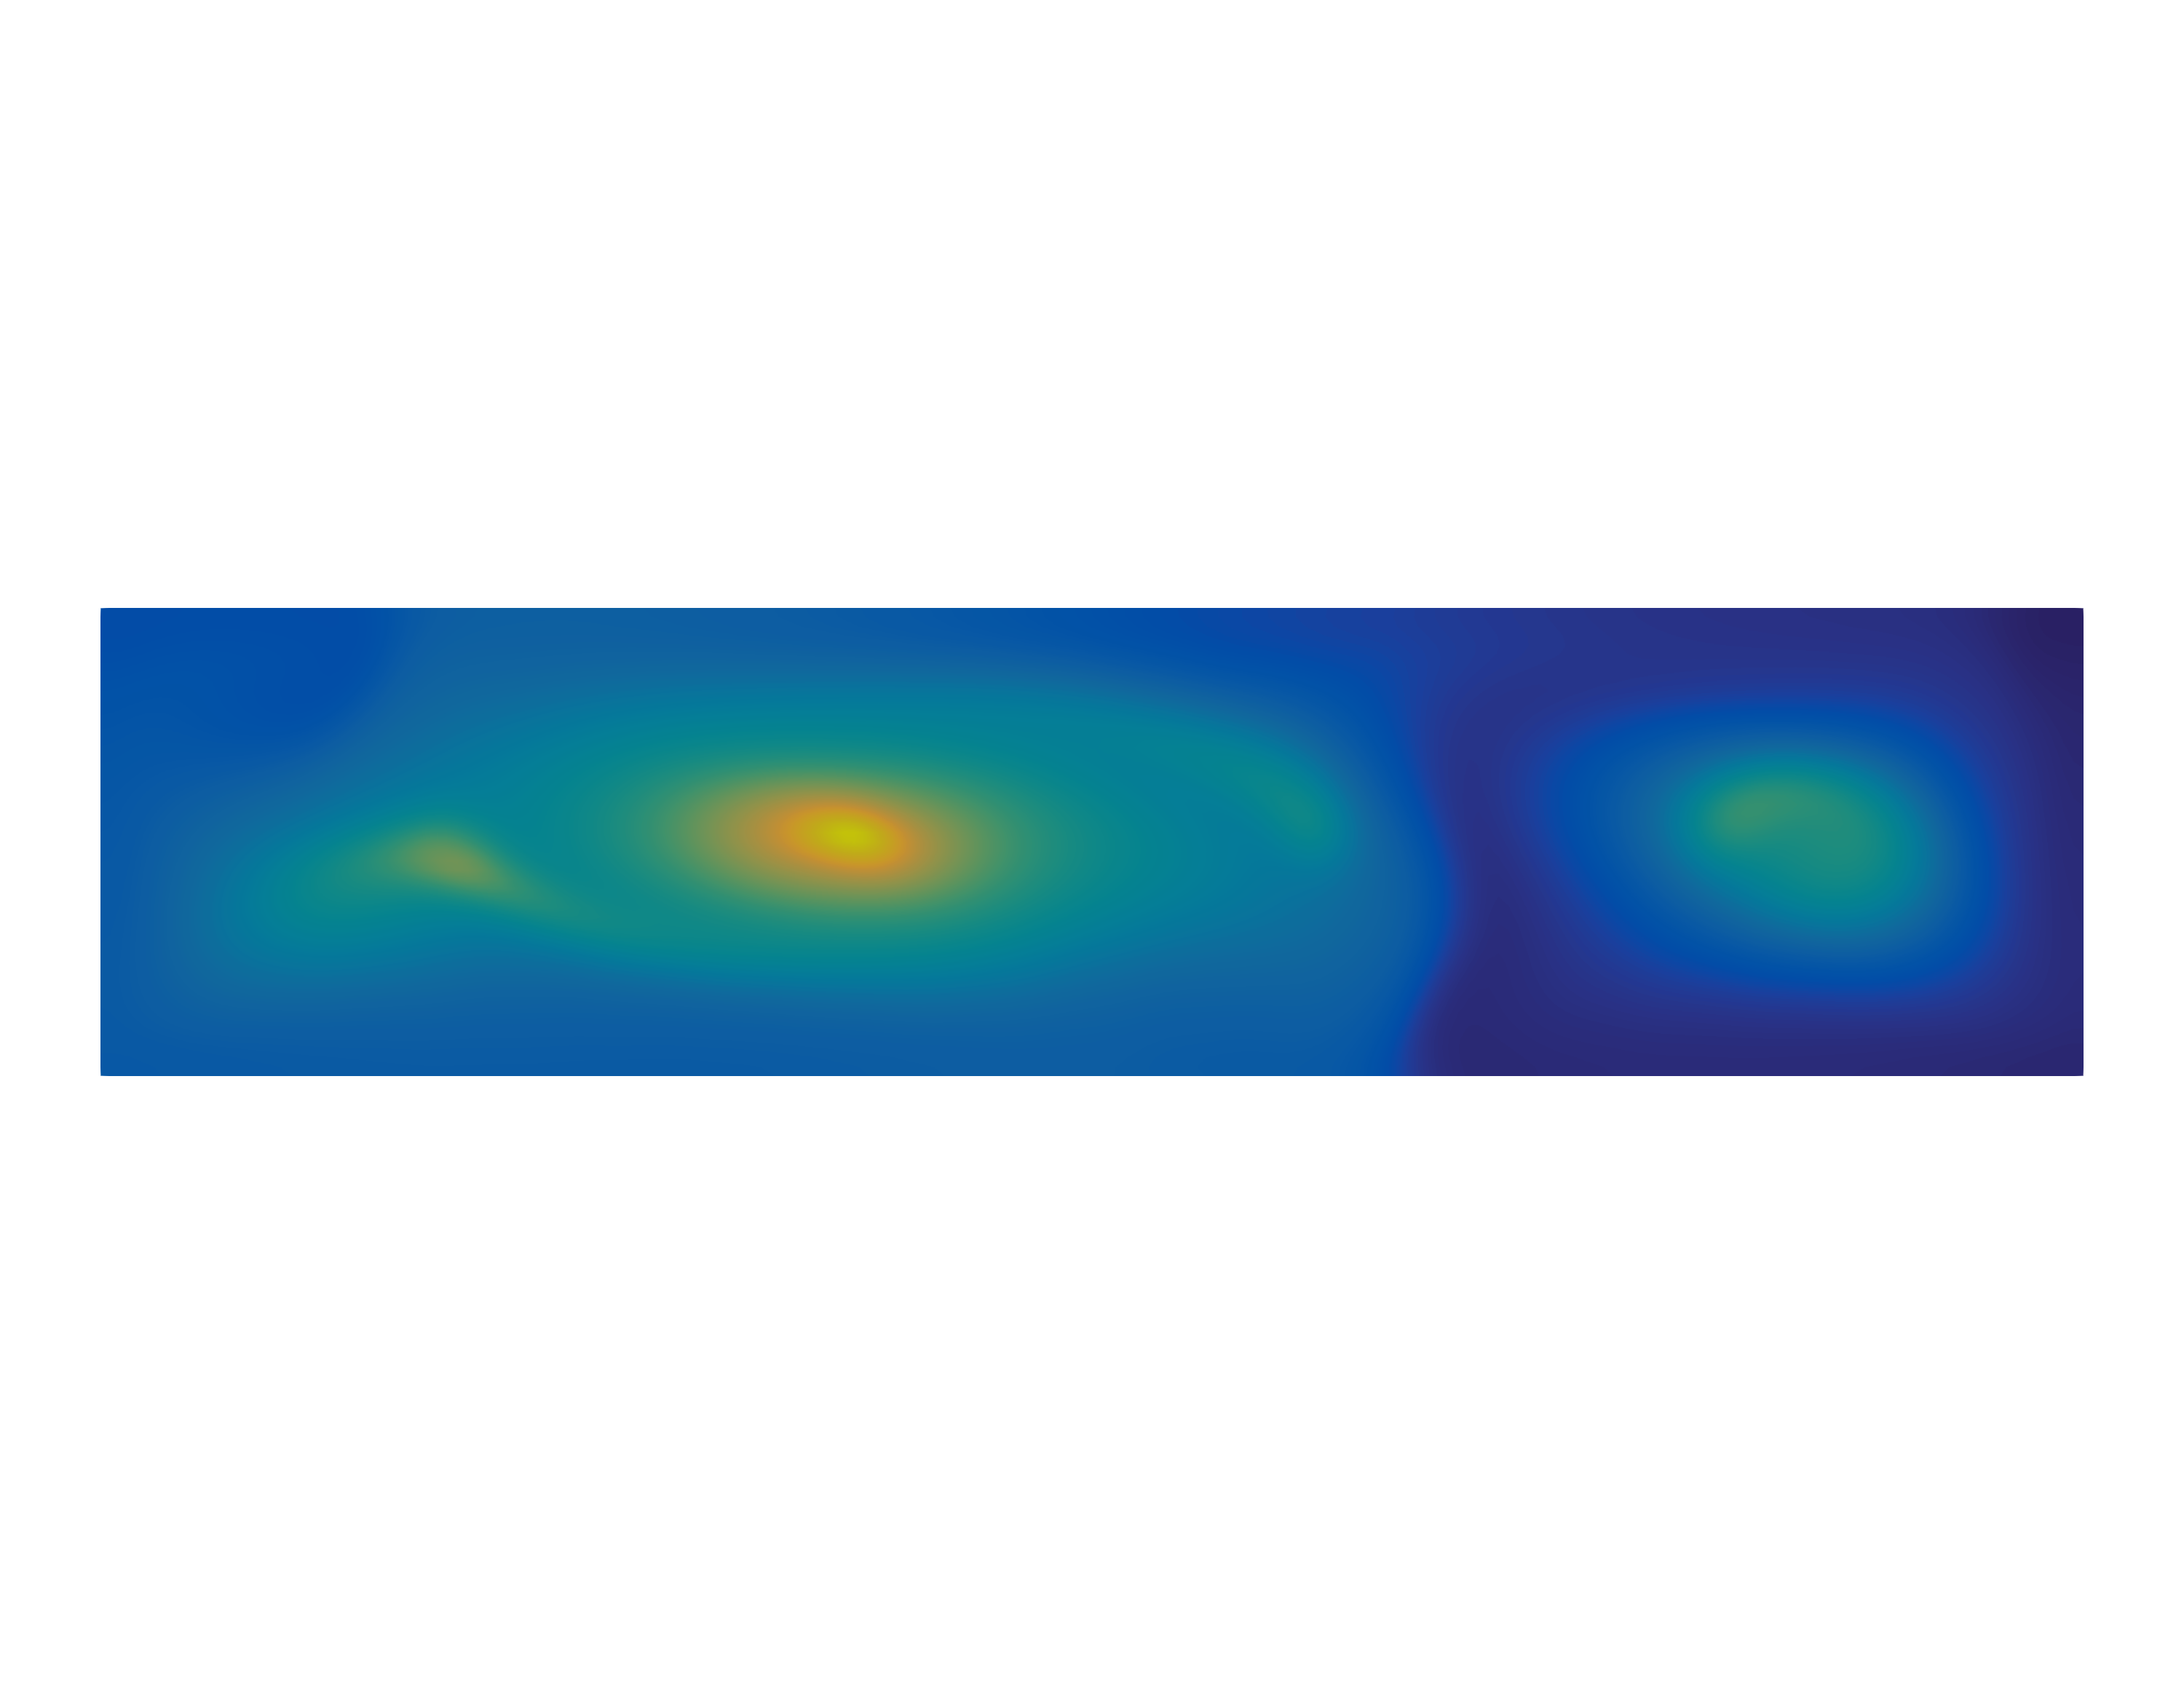
\includegraphics[width=0.99\textwidth]{../media/fourier/application/print/ab-0-1-concentration-harm.png}
        \caption{Anode $(1,1)$ désactivée}
        \label{fig:}
      \end{center}
    \end{subfigure}

    \begin{subfigure}[t]{\textwidth}
      \begin{center}
        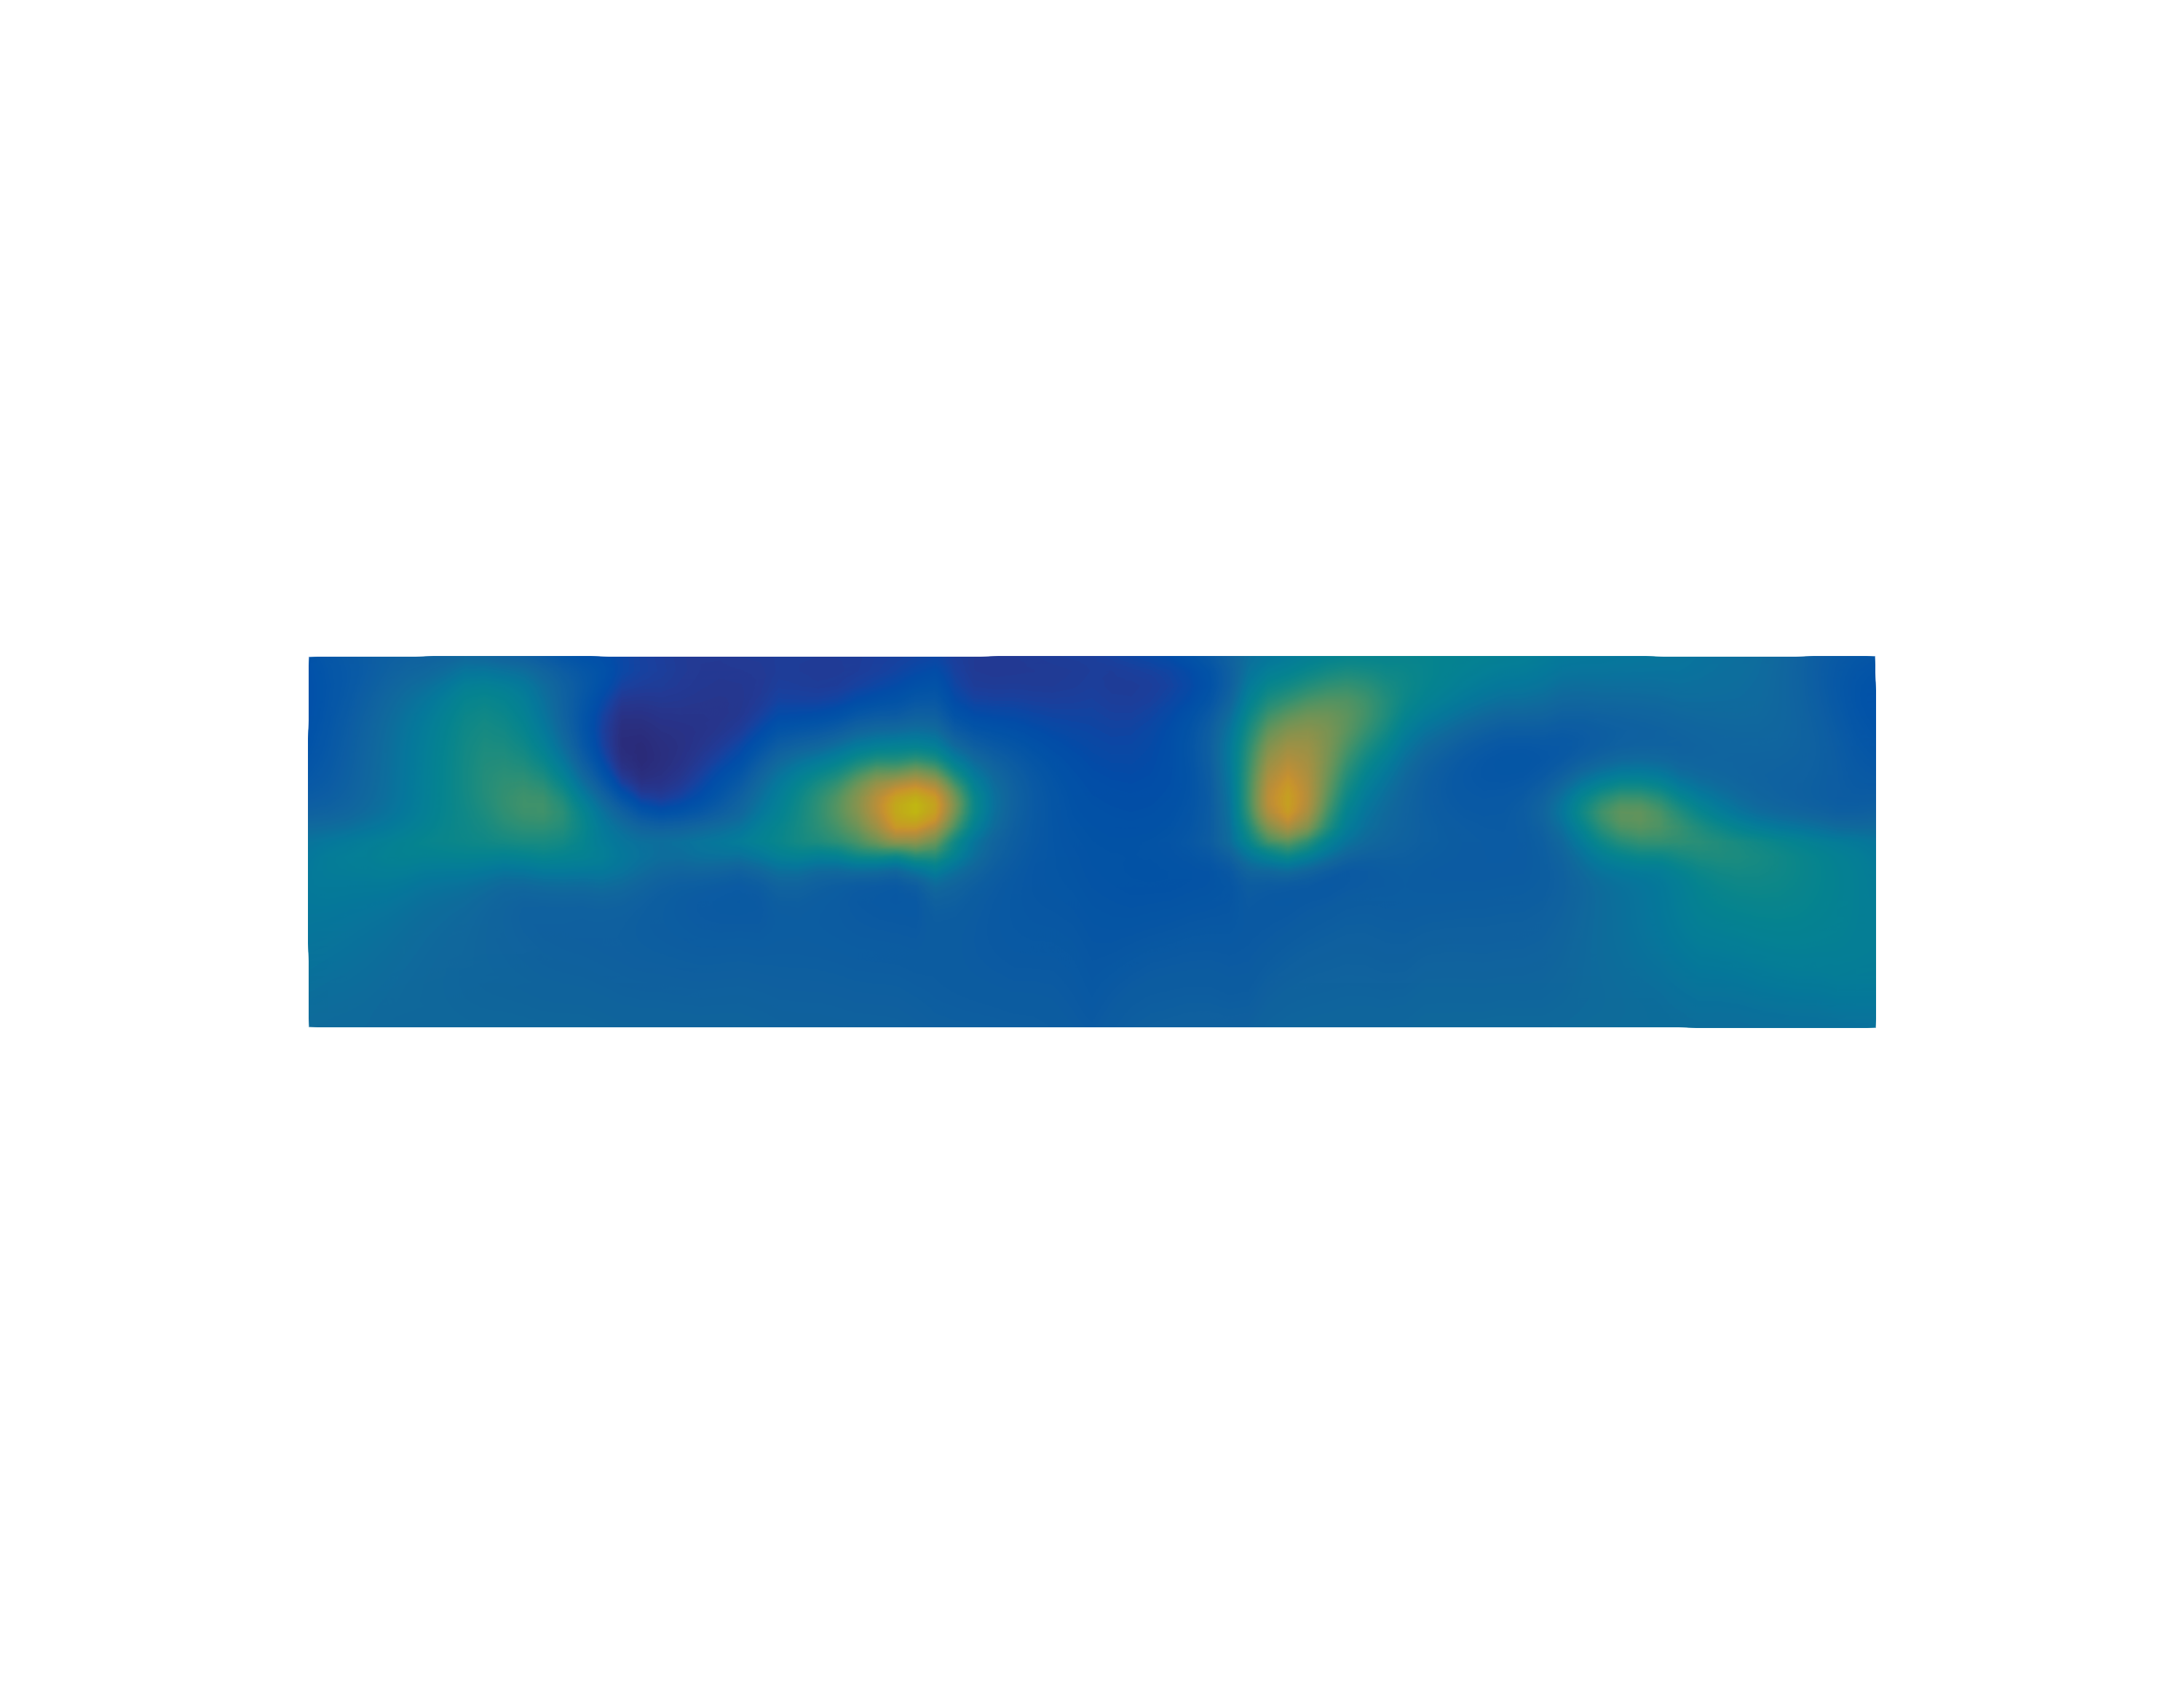
\includegraphics[width=0.99\textwidth]{../media/fourier/application/print/ab-0-2-concentration-acd.png}
        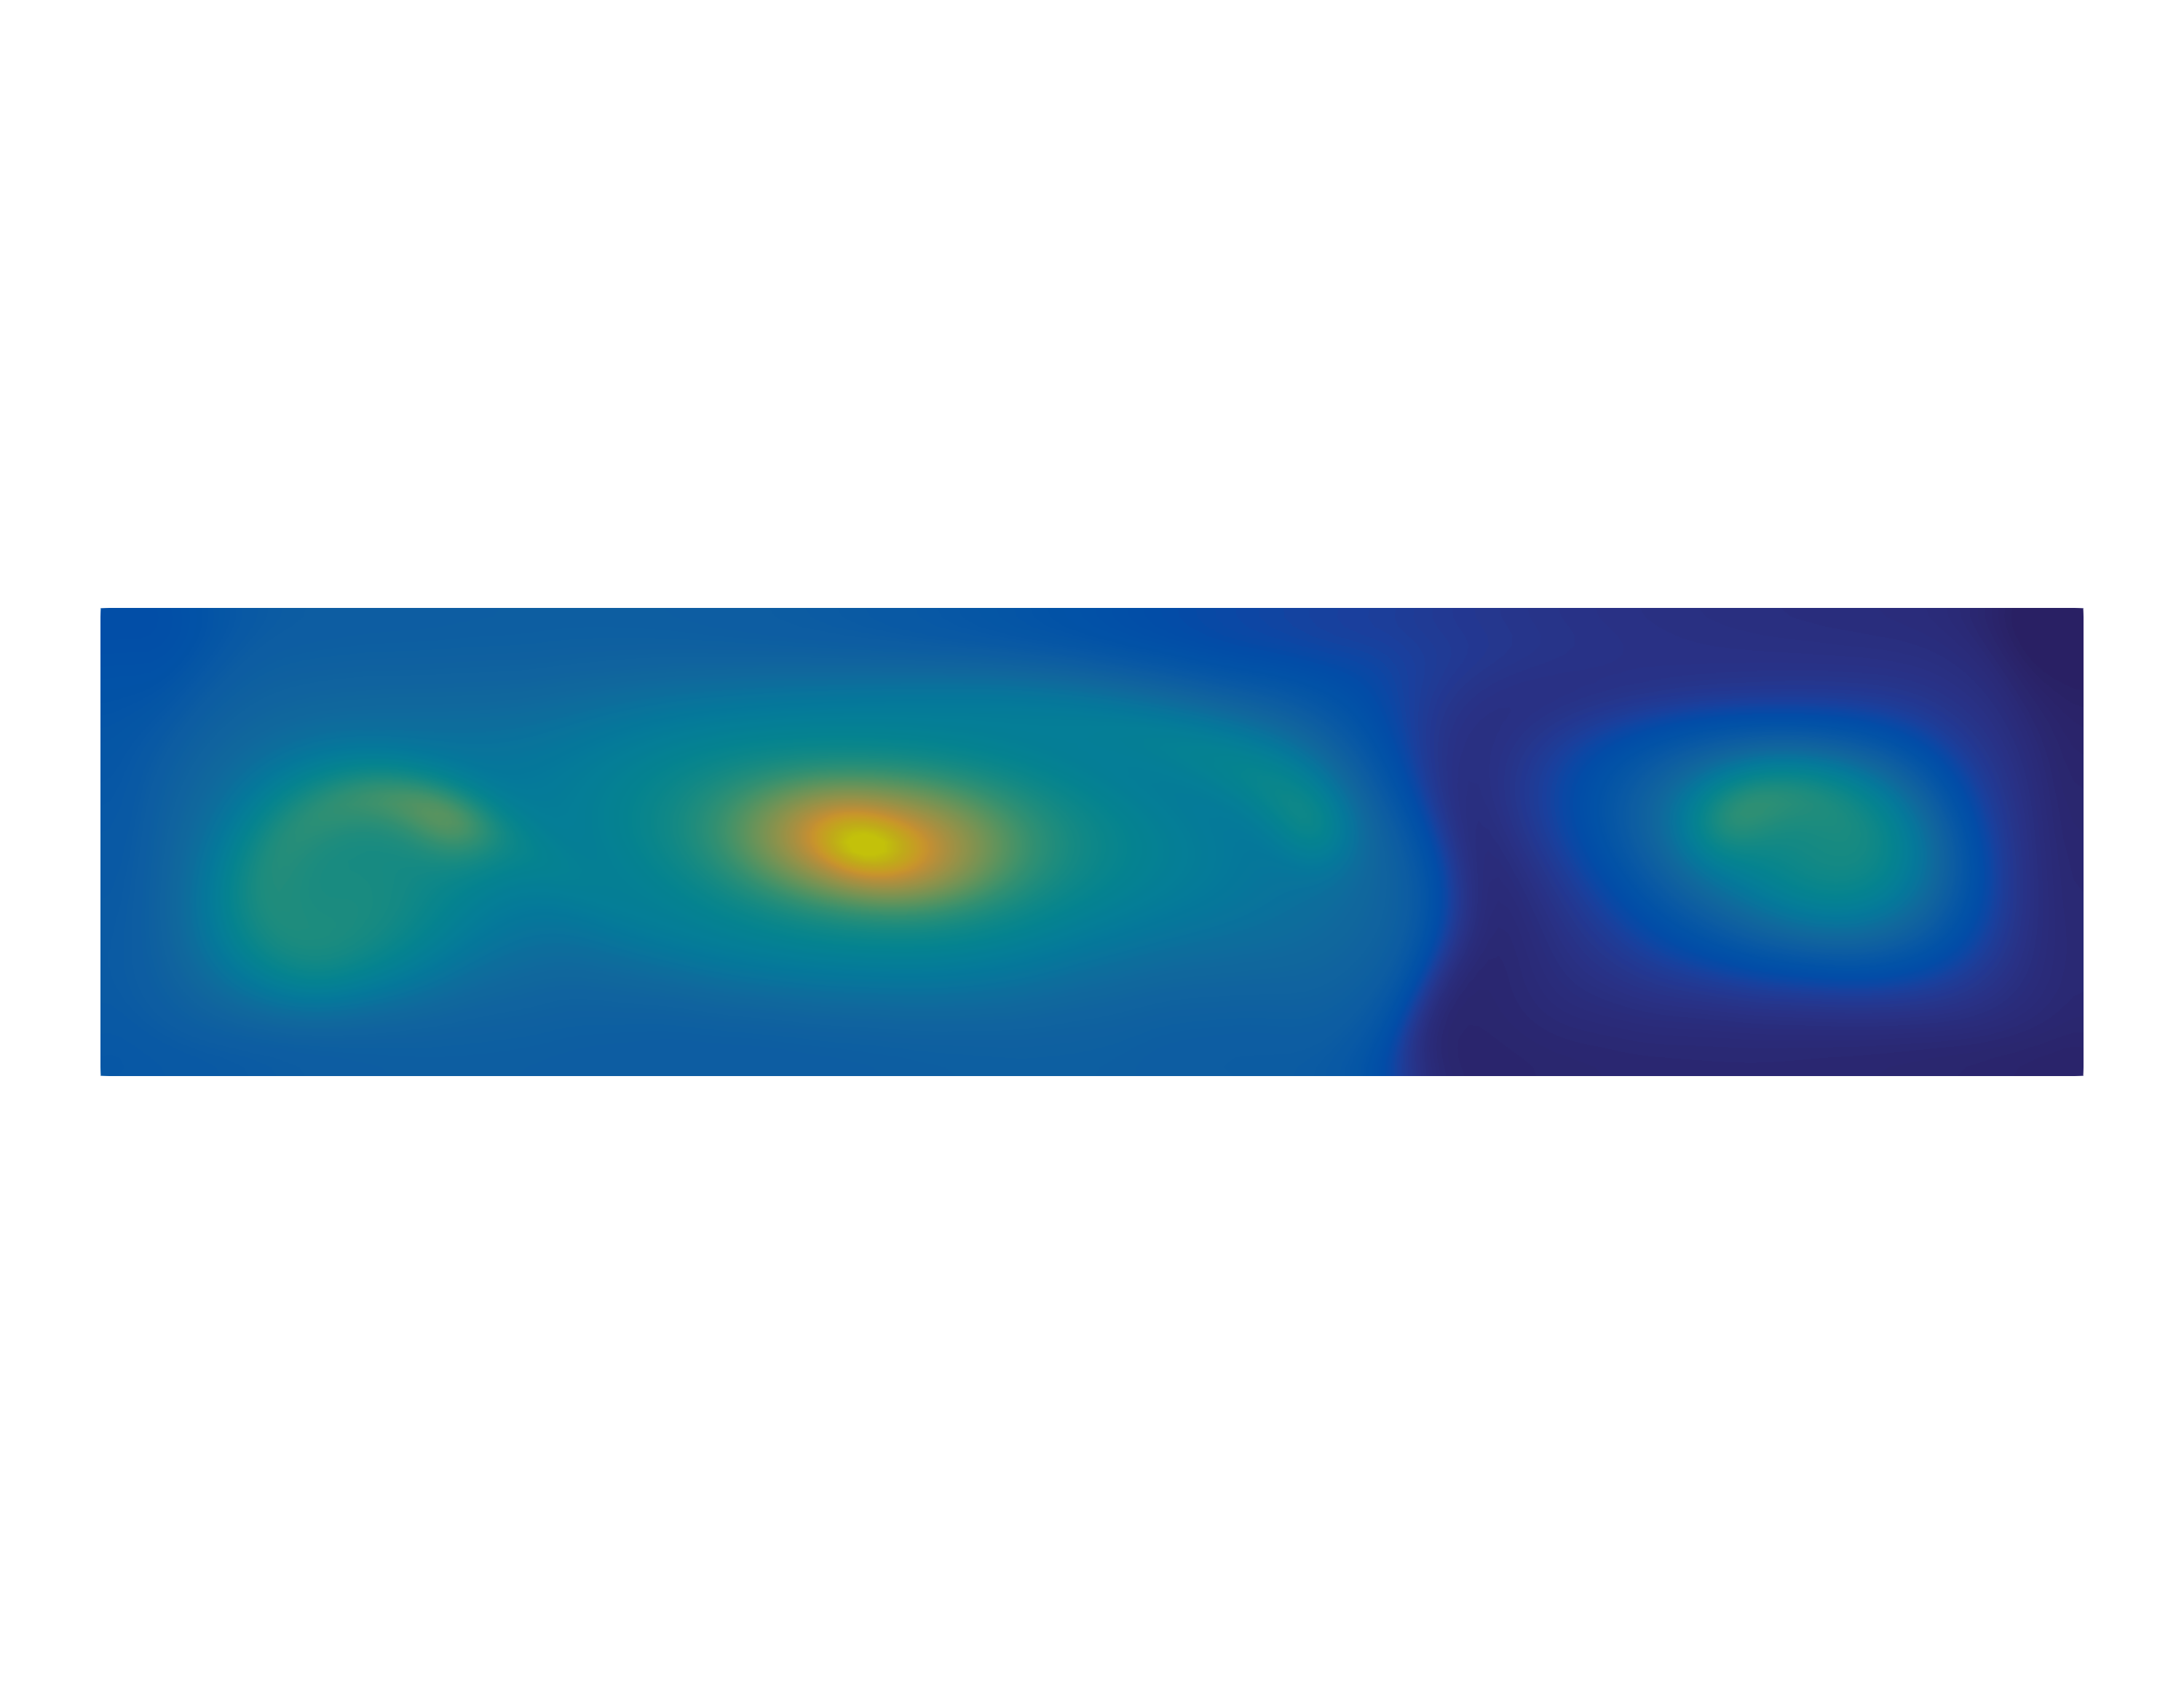
\includegraphics[width=0.99\textwidth]{../media/fourier/application/print/ab-0-2-concentration-harm.png}
        \caption{Anode $(1,2)$ désactivée}
        \label{fig:}
      \end{center}
    \end{subfigure}

    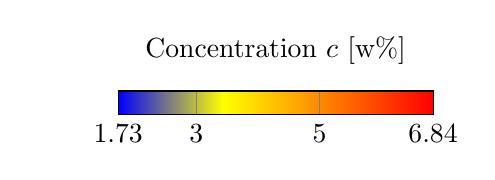
\begin{tikzpicture}
      \begin{axis}[
          colorbar,
          hide axis,
          scale only axis,
          height=0.1\textwidth,
          width=0.5\textwidth,
          colorbar horizontal,
          point meta min=1.73,
          point meta max=6.84,
          colorbar style={
            title=Concentration $c$ [w\%],
            width=4cm,
            height=0.3cm,
            xtick={1.73, 3.0, 5.0, 6.84},
            at={(0.5\textwidth,0.4cm)},
            anchor=north
          }
        ]
        \addplot [] coordinates {(0,0)};
        \node (myfirstpic) at (0,0) {};
      \end{axis}
    \end{tikzpicture}

    \caption{Champ de concentration $c^\mathrm{S3D}$ (haut) et
      $c^\mathrm{SF}$ dans les différentes configurations anodiques.}

    \label{fig:harmonic-concentration-comp-a}
  \end{center}
\end{figure}

\begin{figure}[h!]
  \begin{center}
    \begin{subfigure}[t]{\textwidth}
      \begin{center}
        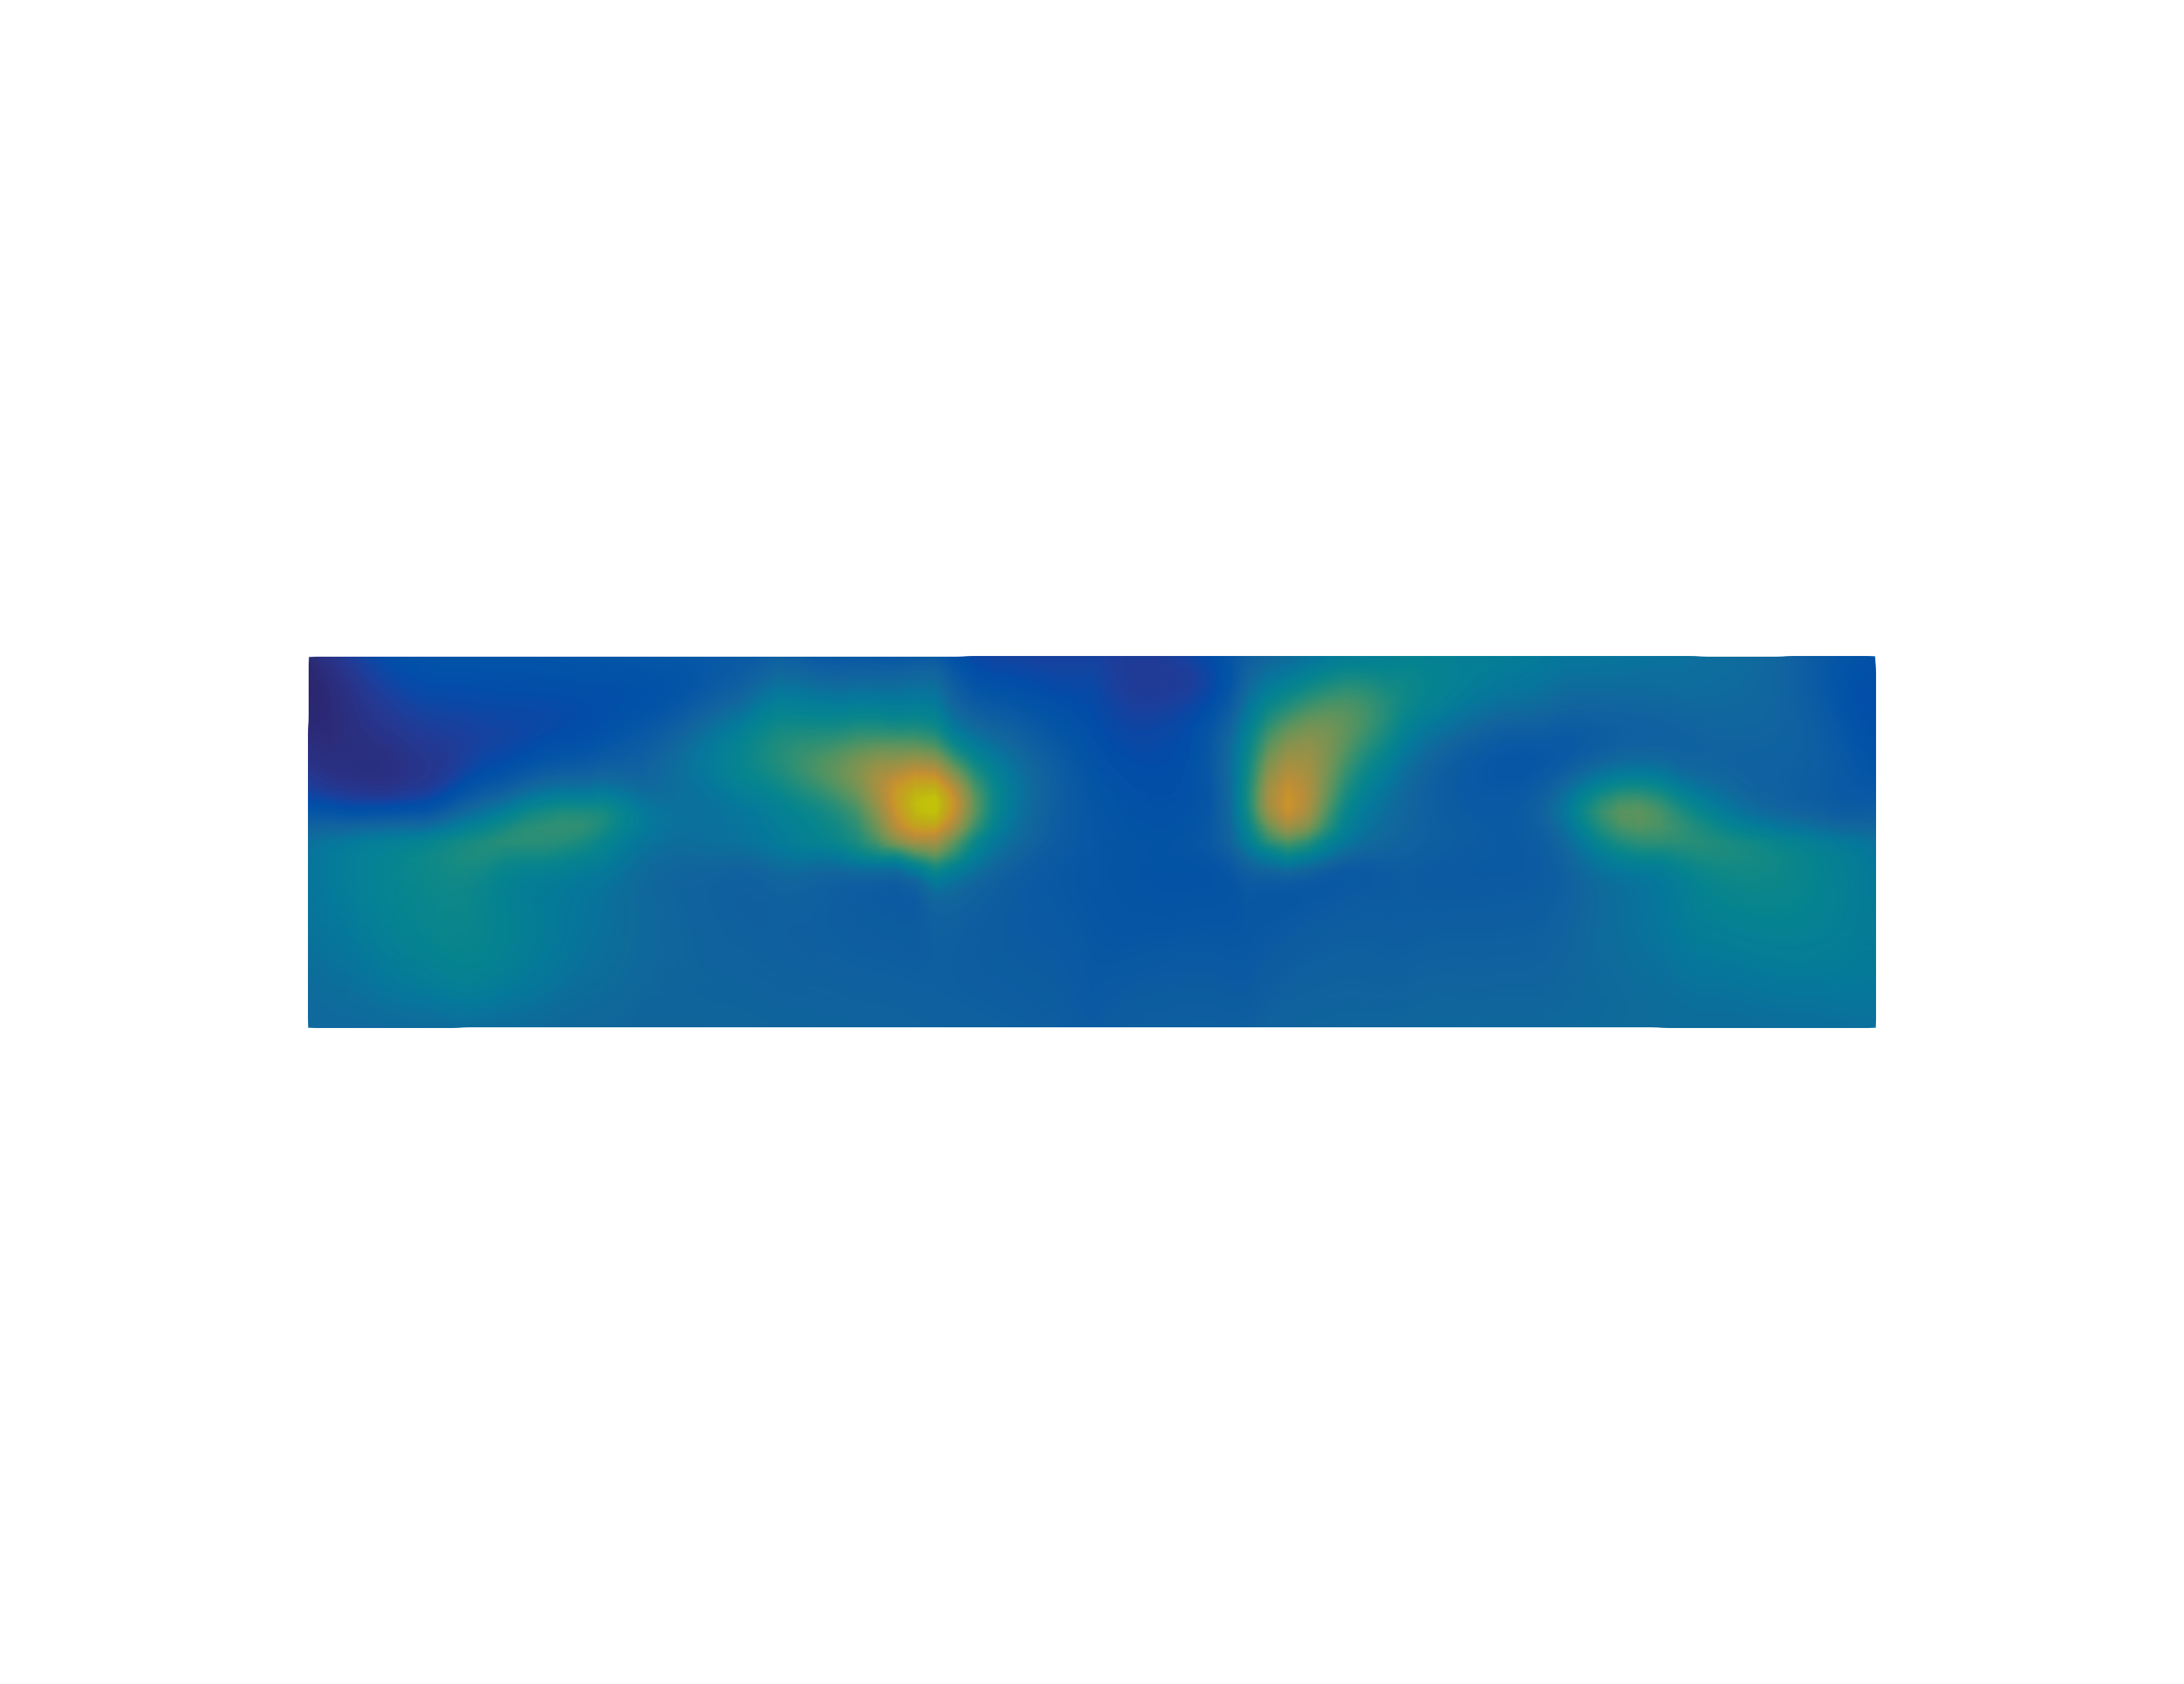
\includegraphics[width=0.99\textwidth]{../media/fourier/application/print/ab-1-1-concentration-acd.png}
        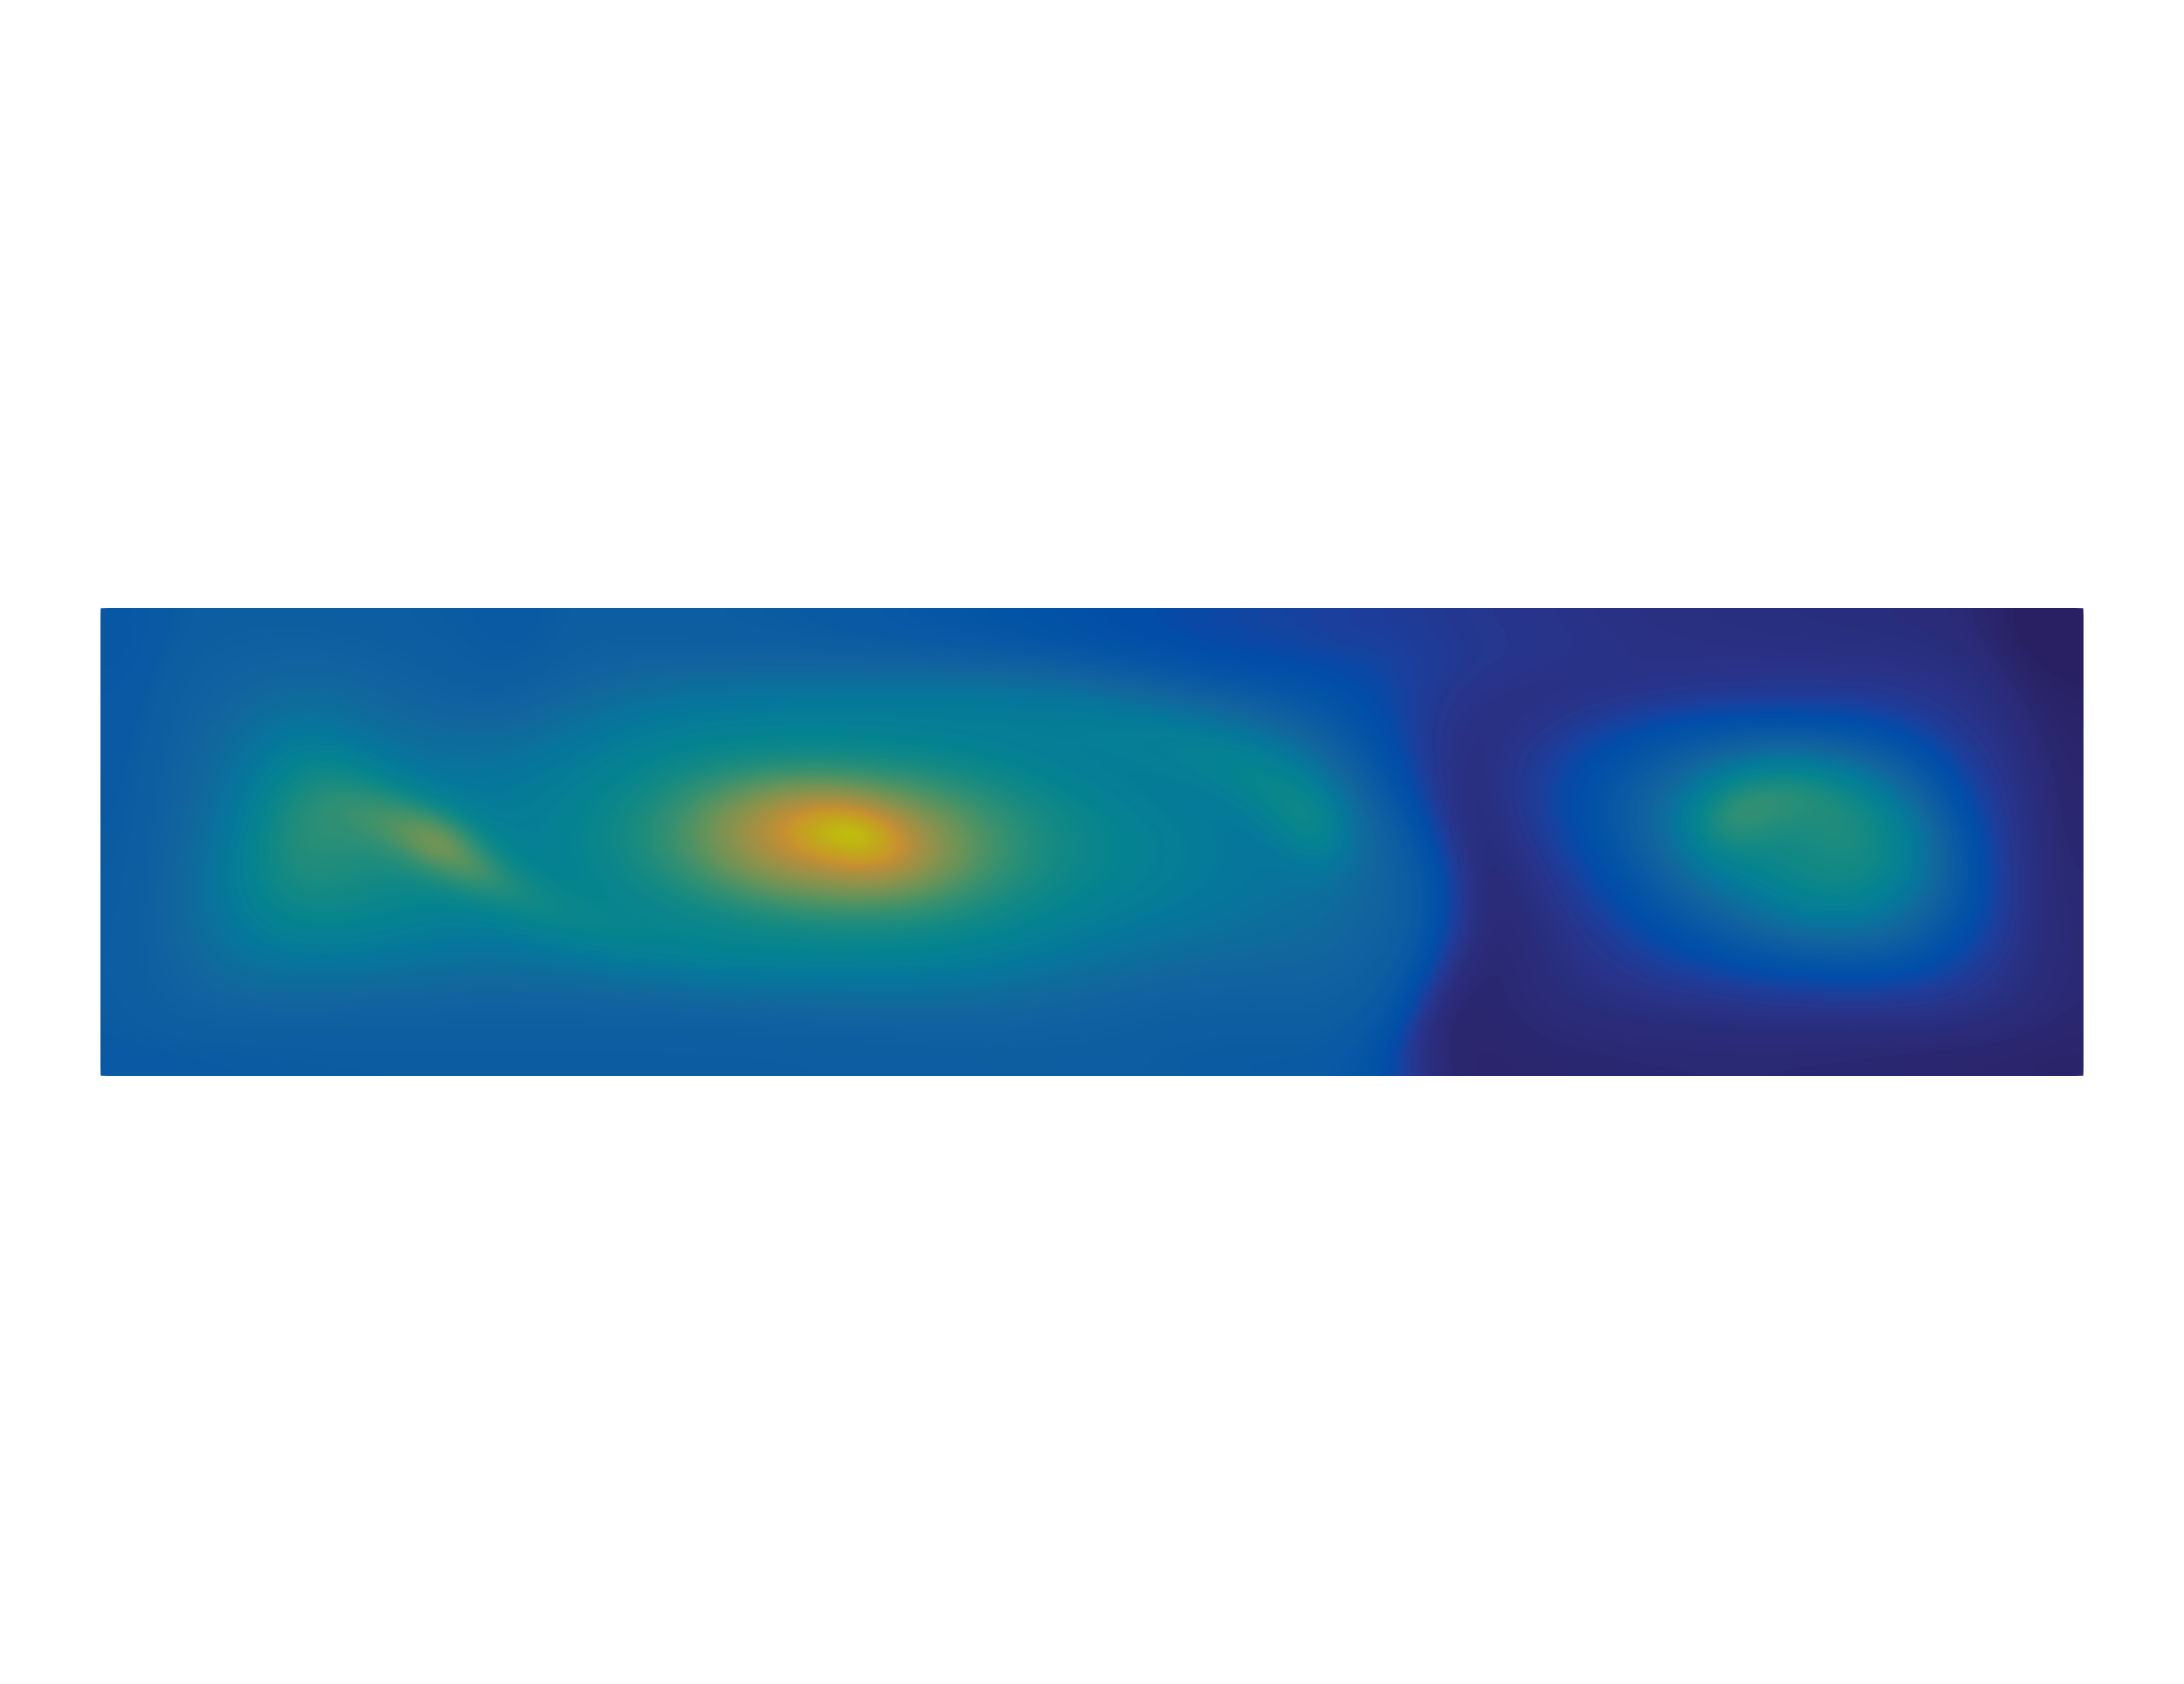
\includegraphics[width=0.99\textwidth]{../media/fourier/application/print/ab-1-1-concentration-harm.png}
        \caption{Anode $(2,1)$ désactivée}
        \label{fig:}
      \end{center}
    \end{subfigure}

    \begin{subfigure}[t]{\textwidth}
      \begin{center}
        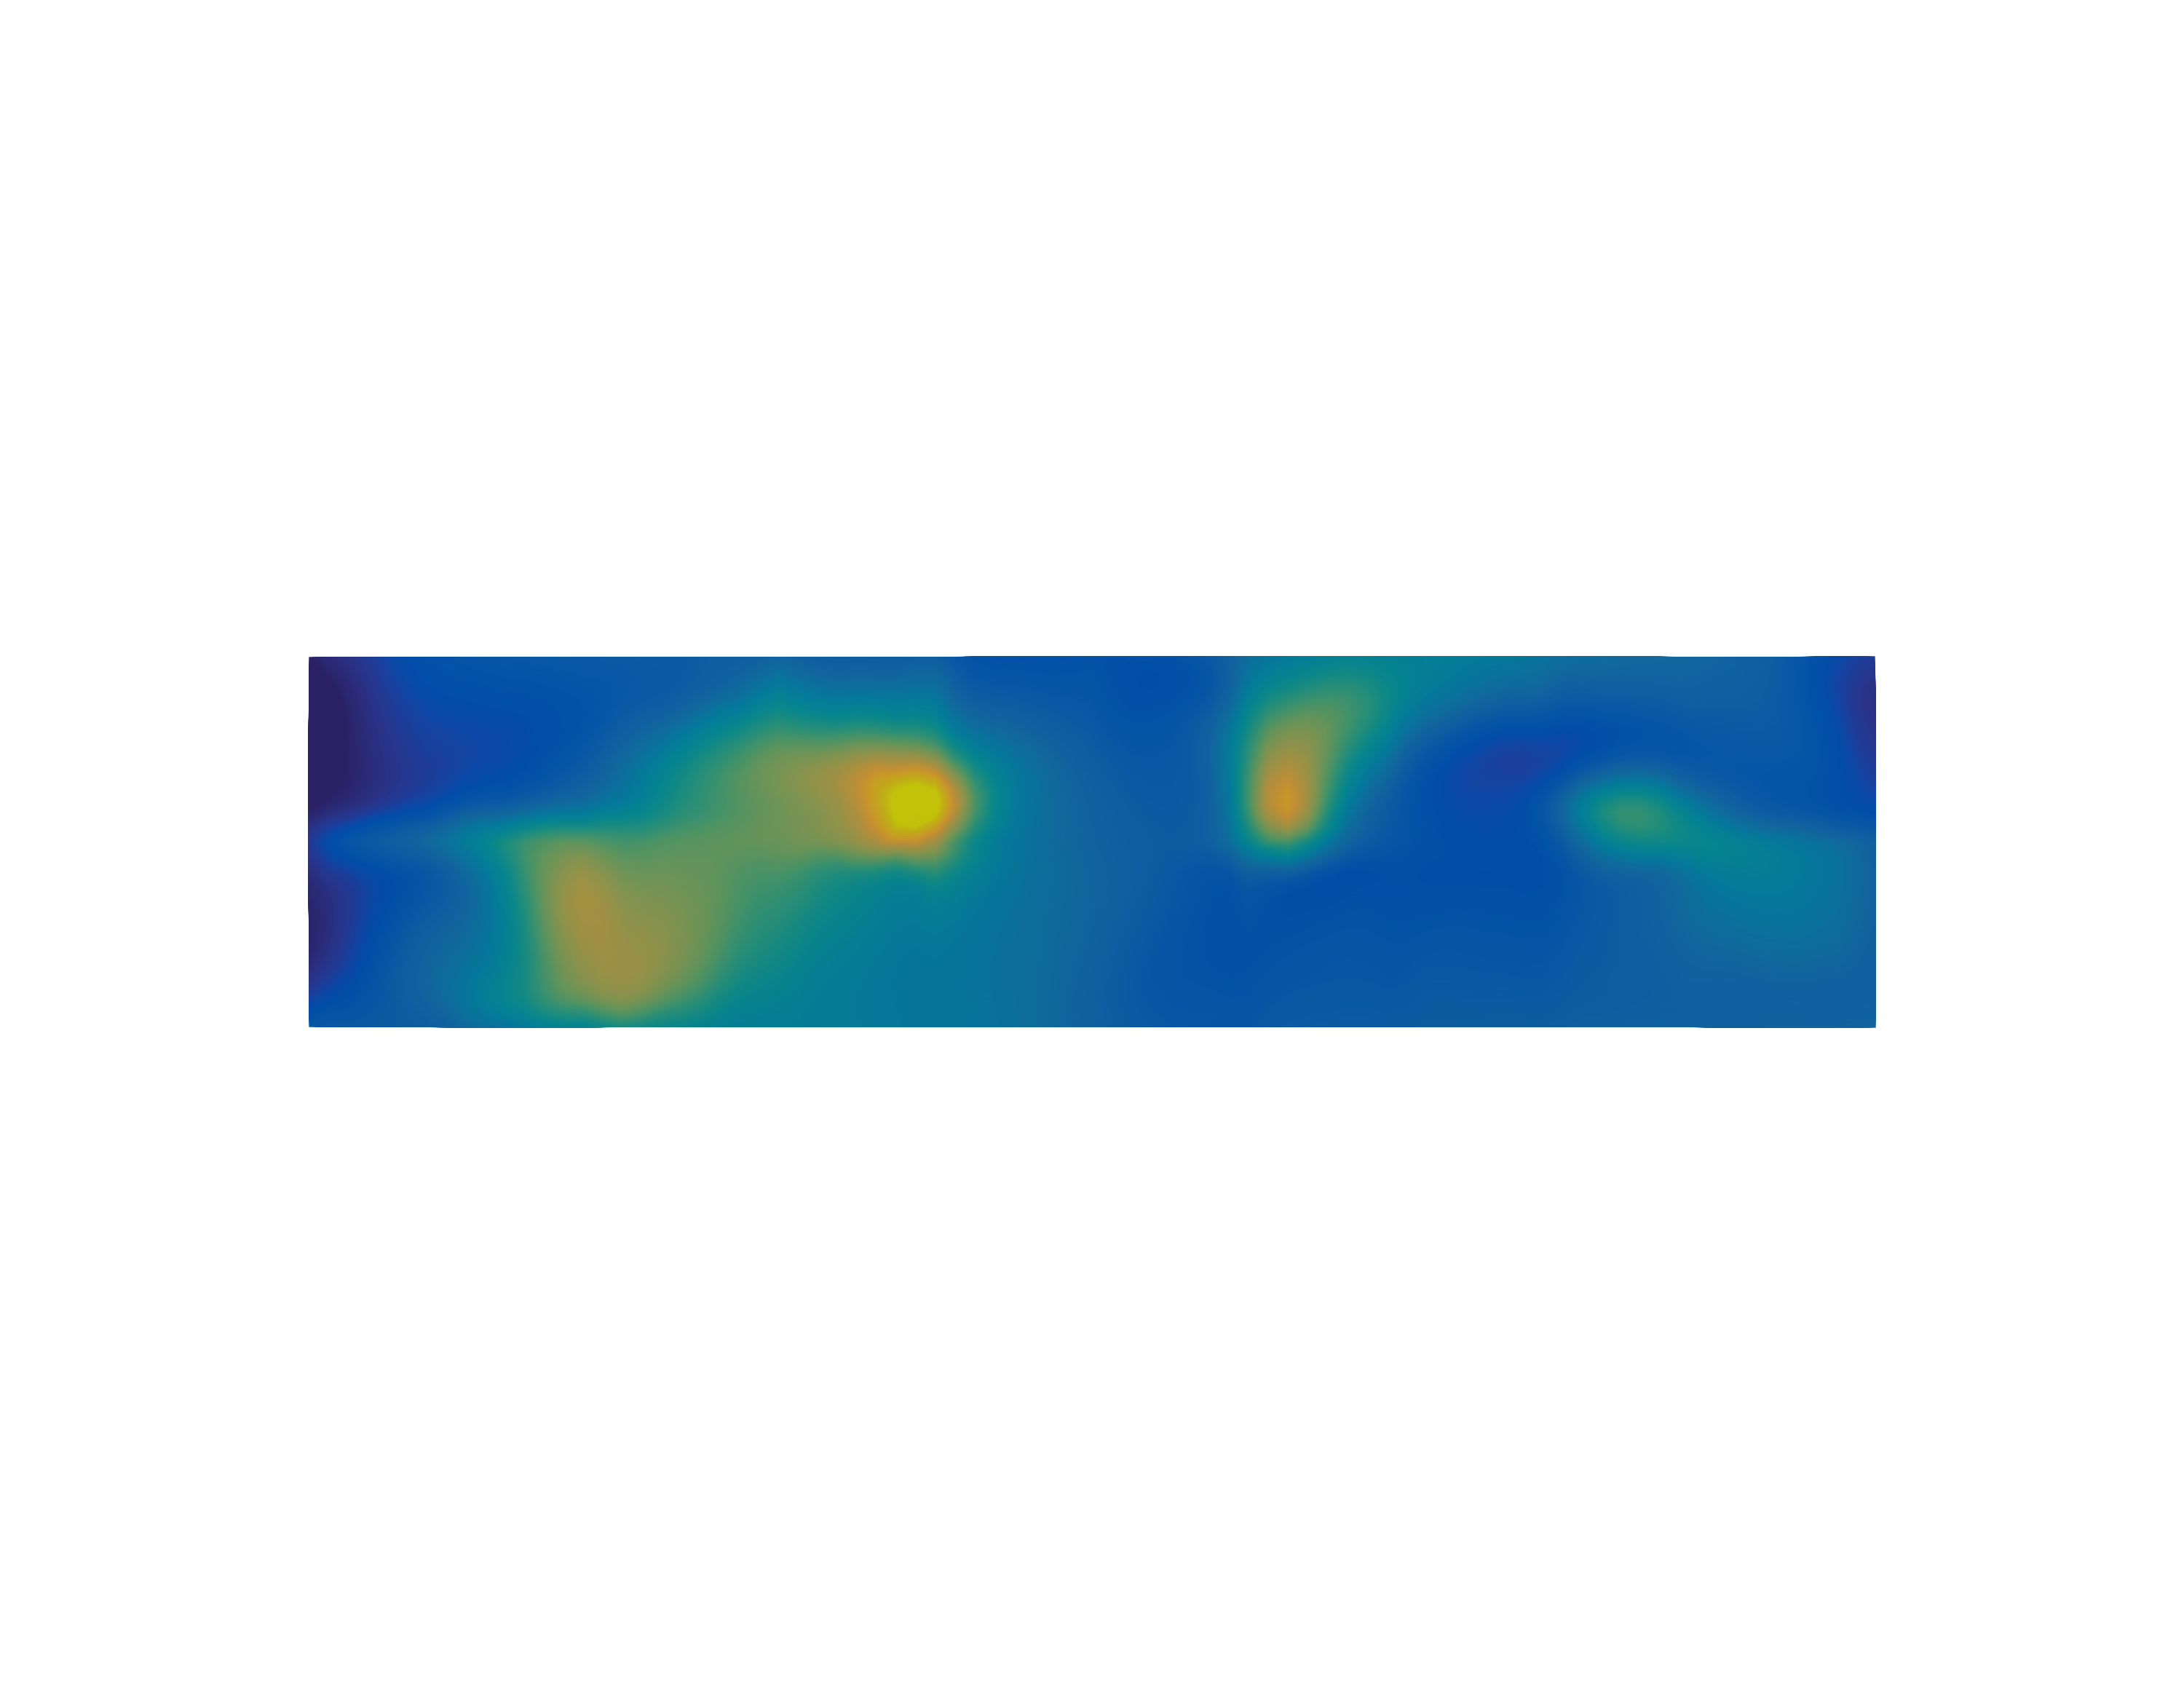
\includegraphics[width=0.99\textwidth]{../media/fourier/application/print/ab-1-2-concentration-acd.png}
        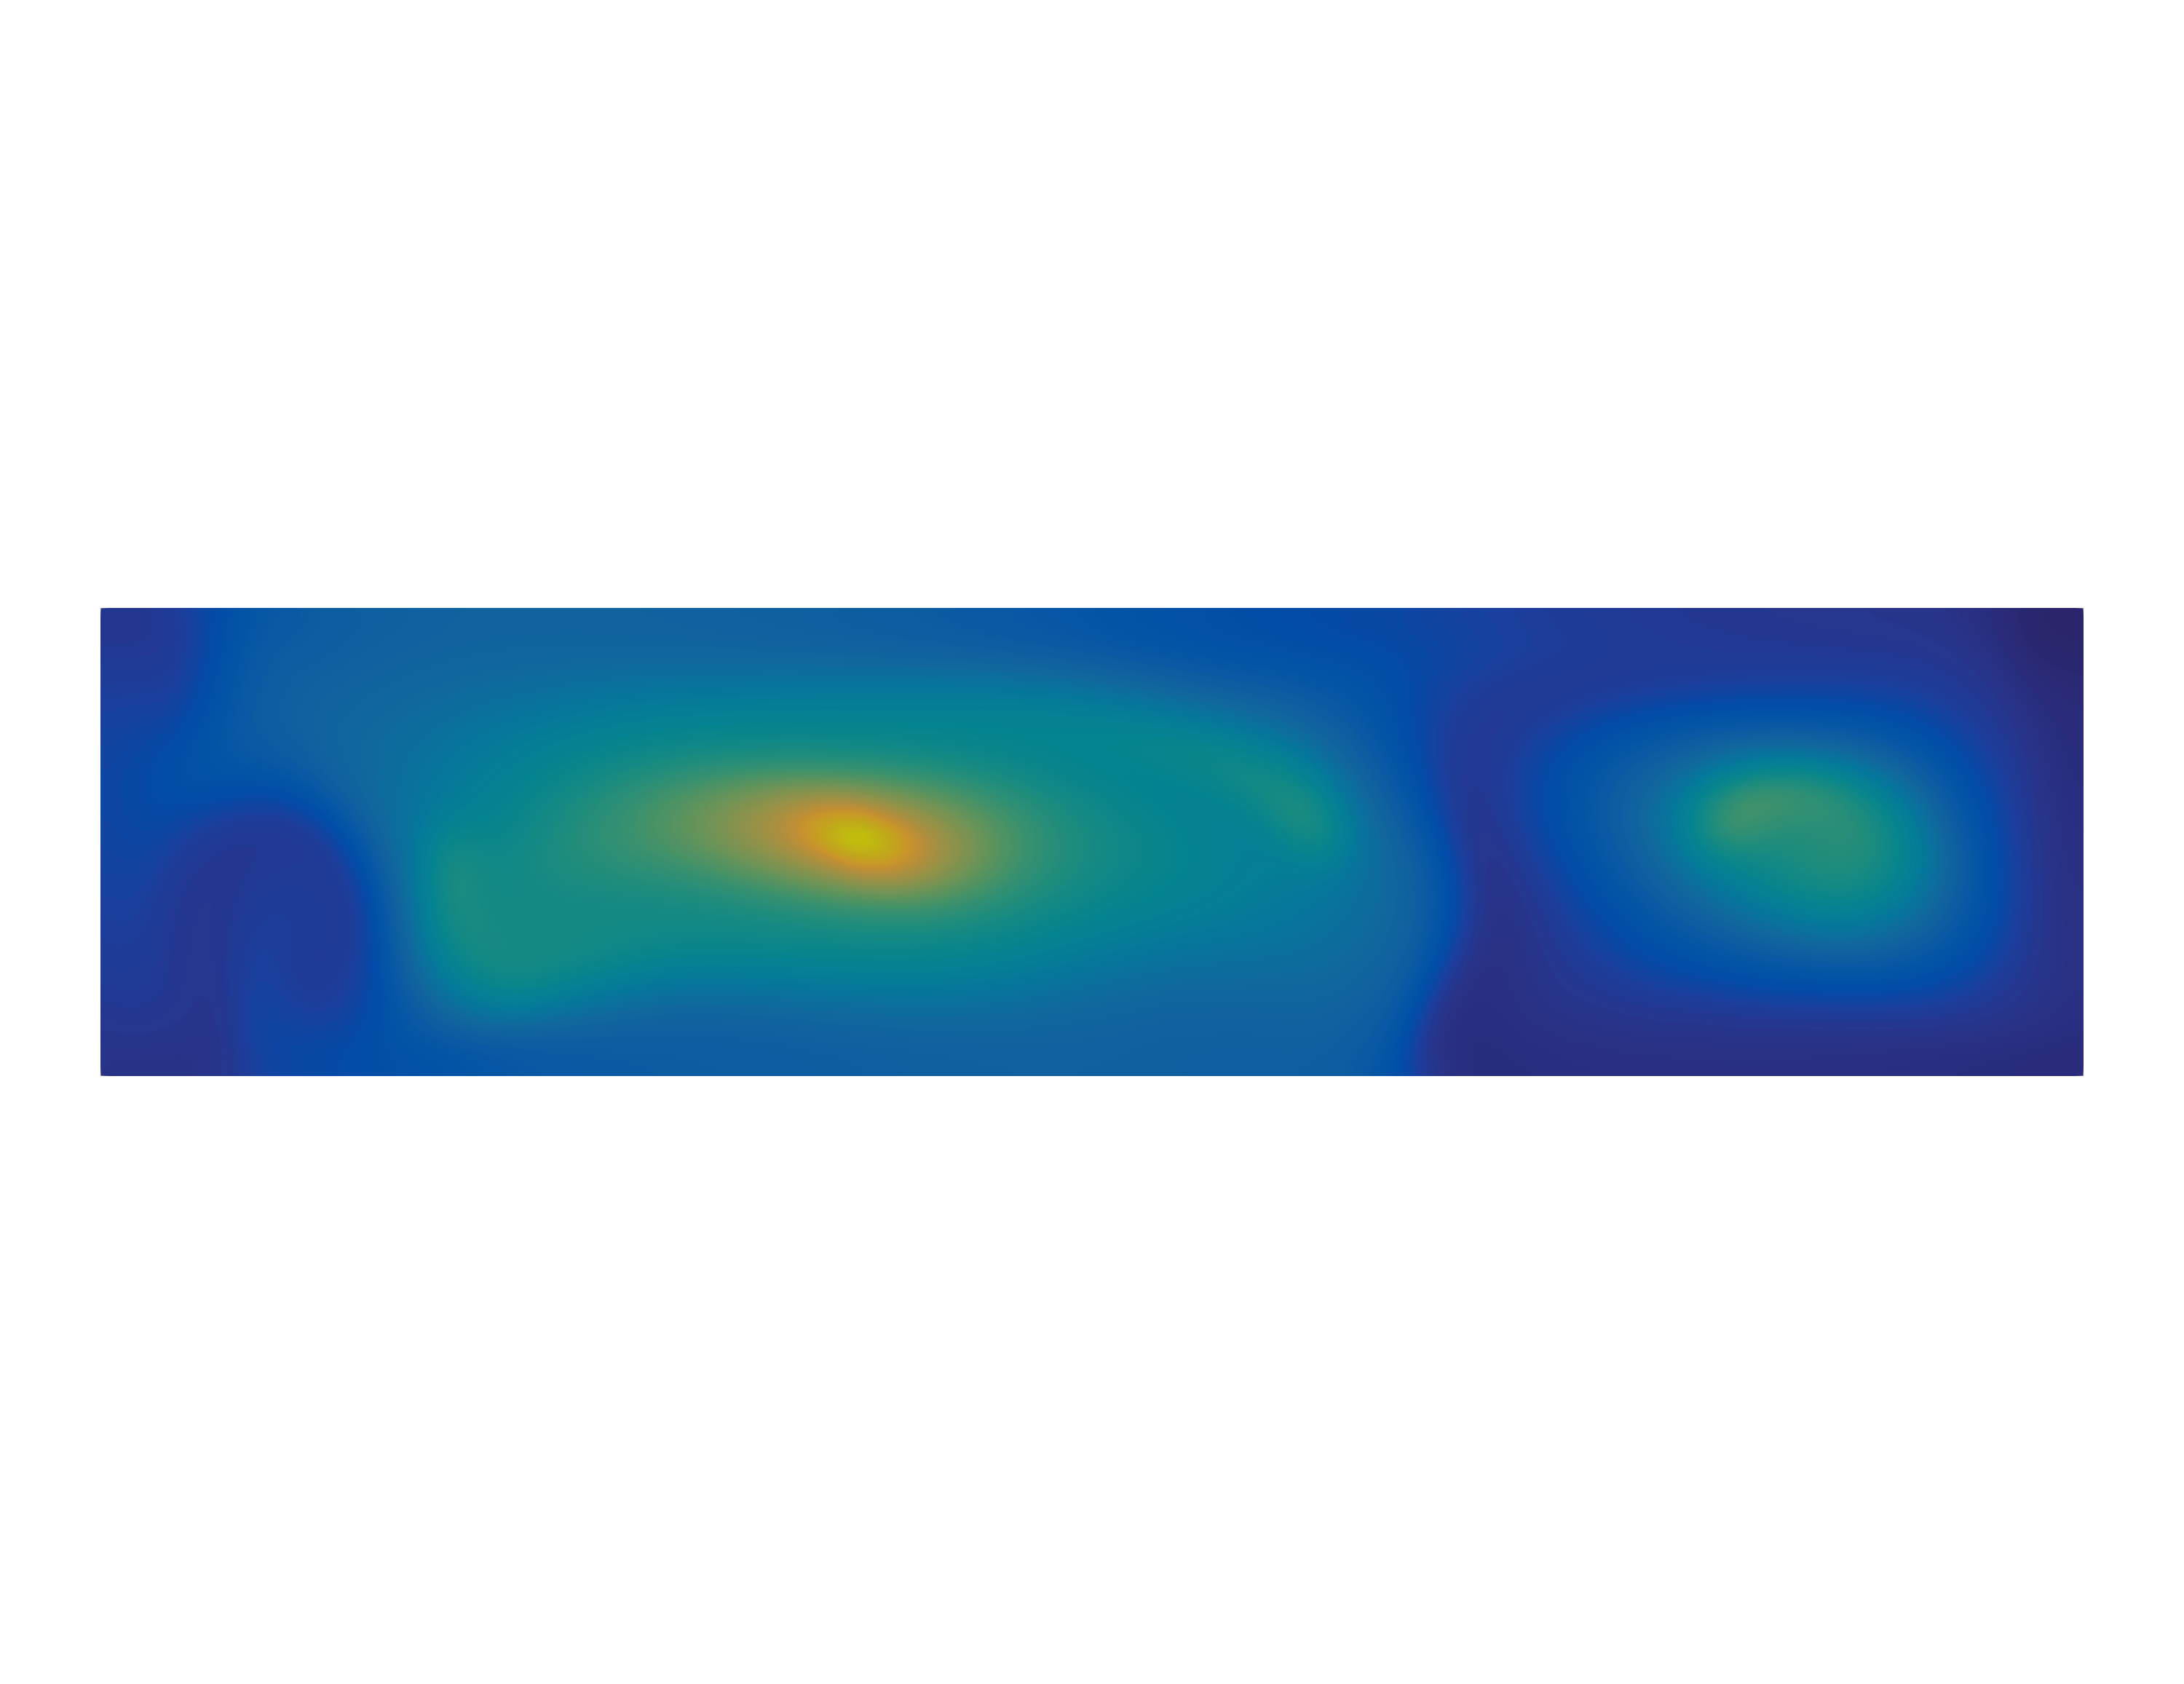
\includegraphics[width=0.99\textwidth]{../media/fourier/application/print/ab-1-2-concentration-harm.png}
        \caption{Anode $(2,2)$ désactivée}
        \label{fig:}
      \end{center}
    \end{subfigure}

    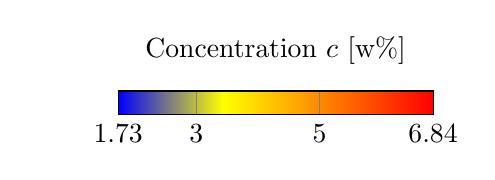
\begin{tikzpicture}
      \begin{axis}[
          colorbar,
          hide axis,
          scale only axis,
          height=0.1\textwidth,
          width=0.5\textwidth,
          colorbar horizontal,
          point meta min=1.73,
          point meta max=6.84,
          colorbar style={
            title=Concentration $c$ [w\%],
            width=4cm,
            height=0.3cm,
            xtick={1.73, 3.0, 5.0, 6.84},
            at={(0.5\textwidth,0.4cm)},
            anchor=north
          }
        ]
        \addplot [] coordinates {(0,0)};
        \node (myfirstpic) at (0,0) {};
      \end{axis}
    \end{tikzpicture}

    \caption{Champ de concentration $c^\mathrm{S3D}$ (haut) et
      $c^\mathrm{SF}$ dans les différentes configurations anodiques.}

    \label{fig:harmonic-concentration-comp-b}
  \end{center}
\end{figure}

Lorsqu'une anodes est désactivée, elle ne conduit plus le courant
électrique, et par conséquent la densité de courant électrique
responsable de la force de Lorentz dans le fluide est fortement
réduite sous l'anode concernée.

On propose d'approximer le champ de force $f$ à partir de $f^0$ en
annulant celle-ci dans la région située sous l'anode désactivée
(figure \ref{fig:anode-deactivation}b.2). Sur la figure
\ref{fig:harmonic-concentration-comp-fc}, on peut comparer les champs
de concentration dans les différentes configurations anodique entre le
modèle S3D et le modèle SF.


\begin{figure}[h!]
  \begin{center}
    \begin{subfigure}[t]{\textwidth}
      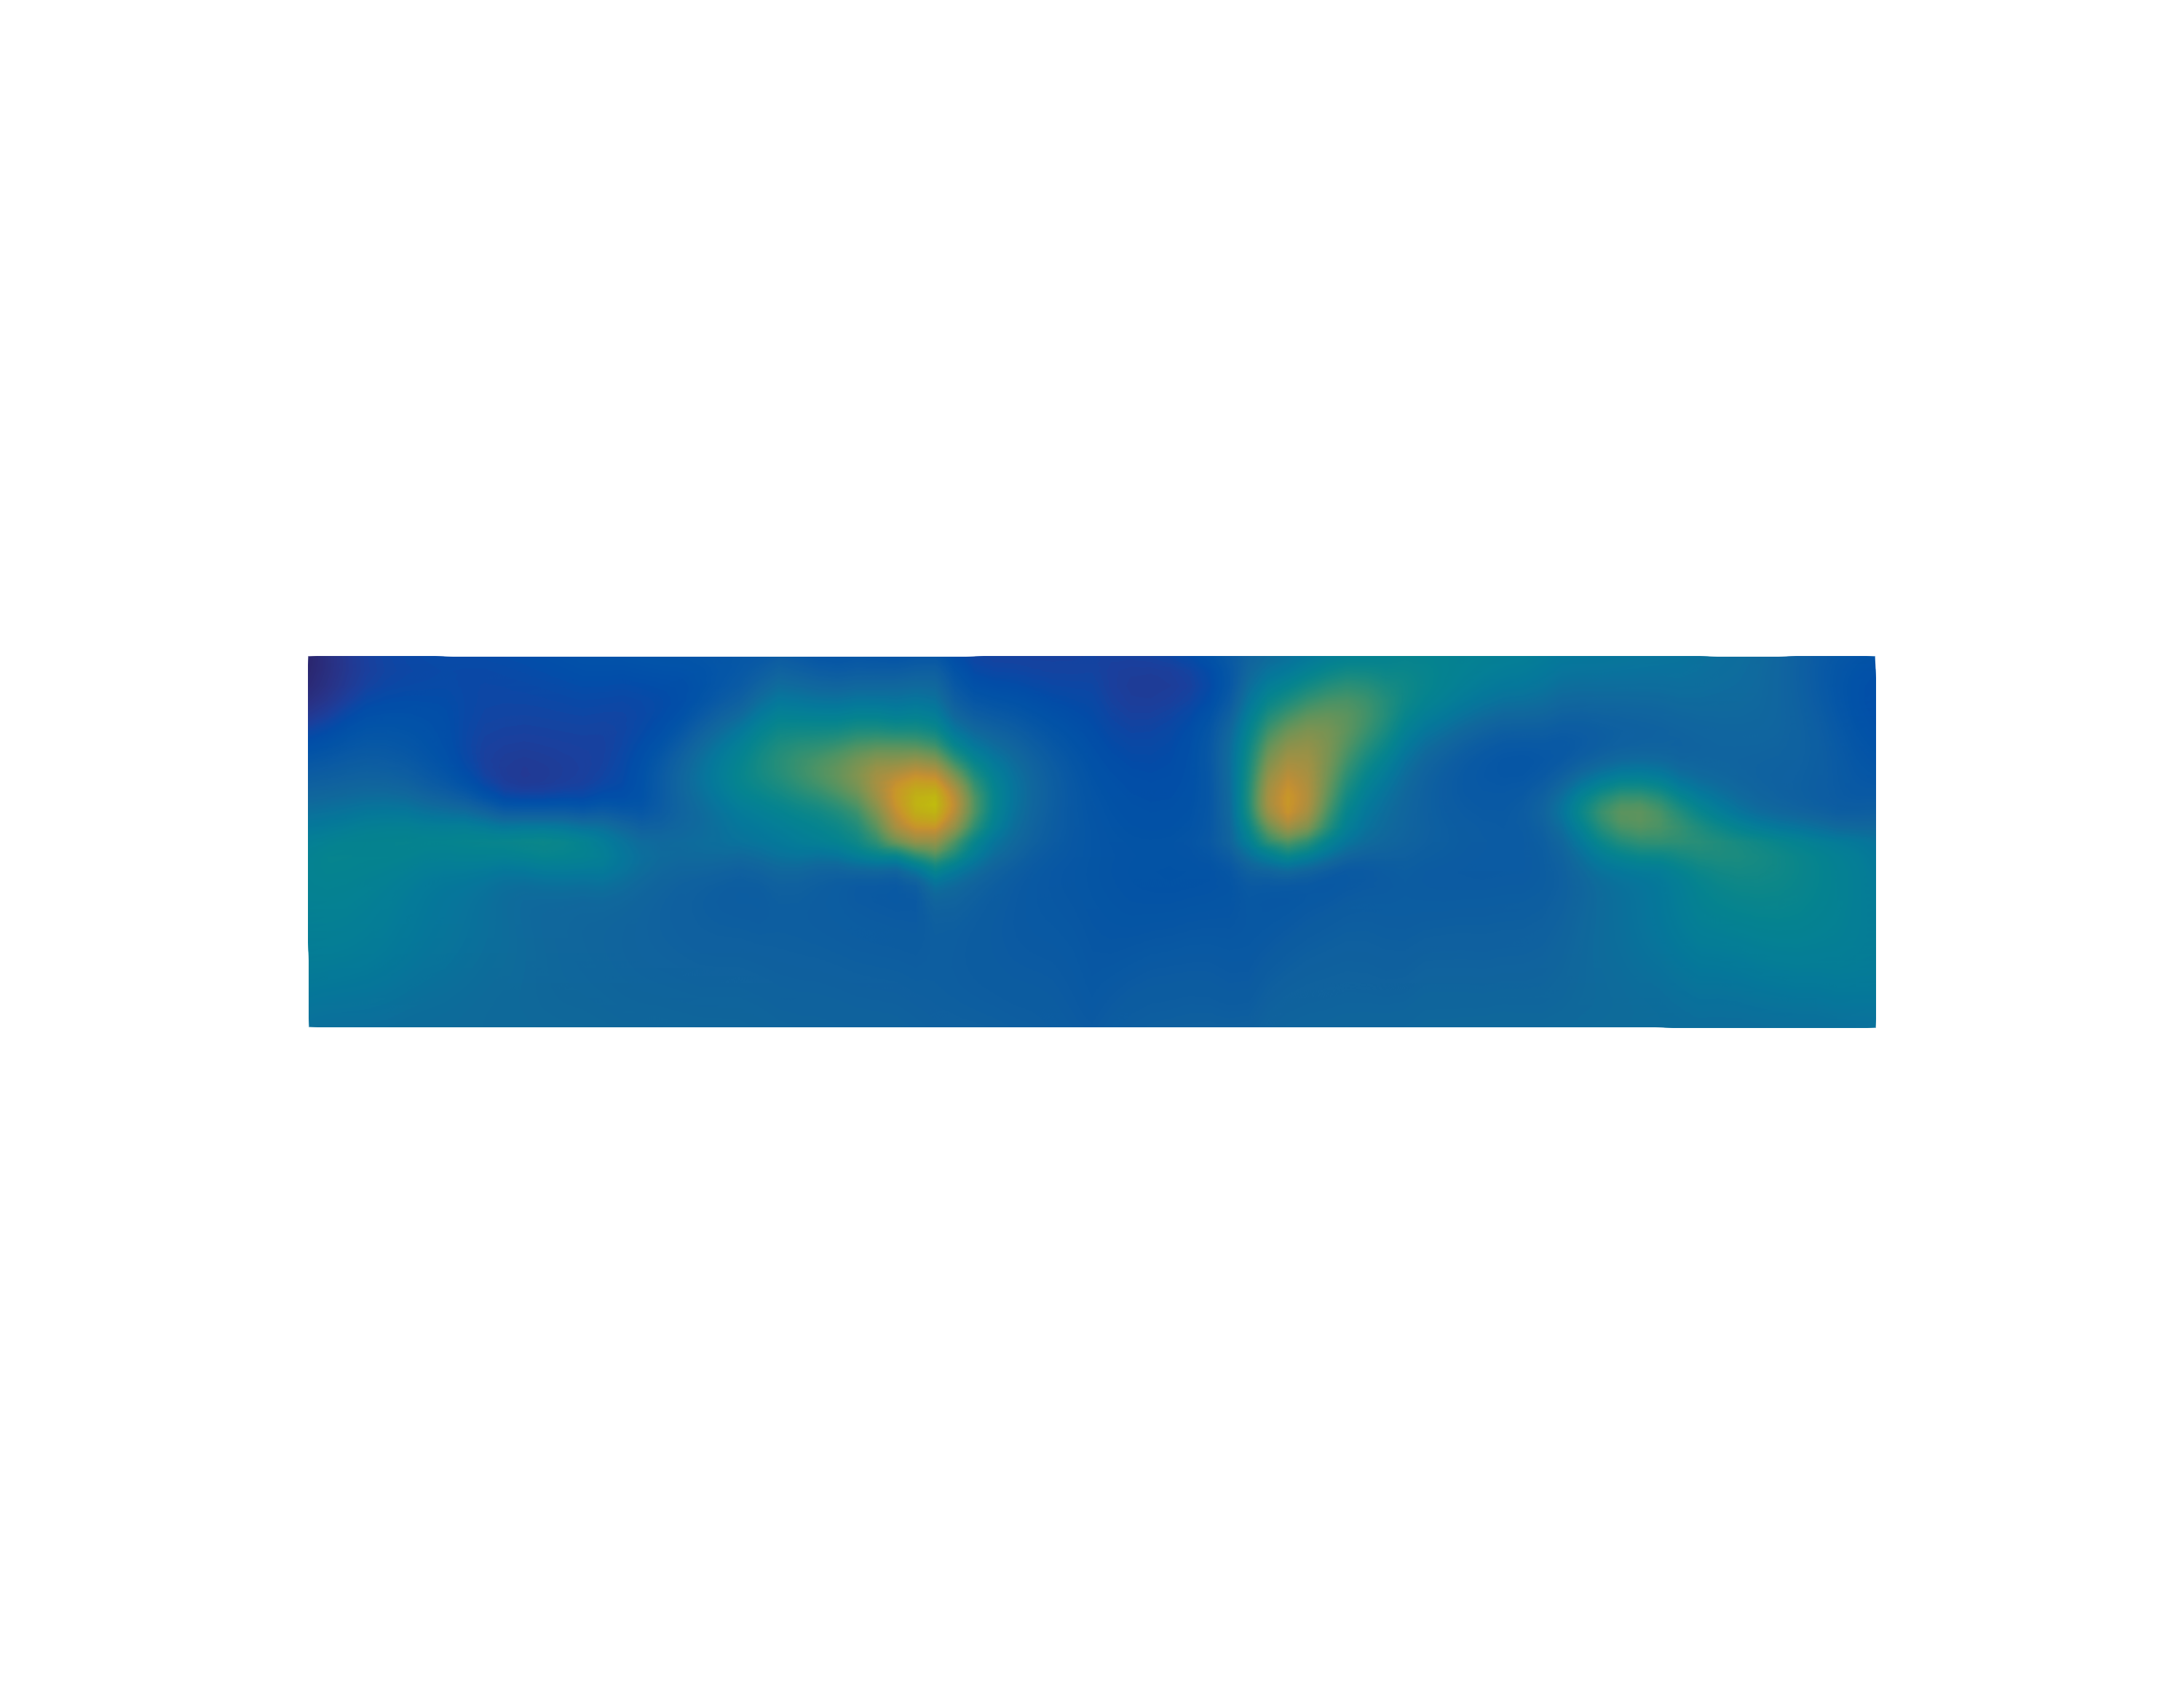
\includegraphics[width=0.99\textwidth]{../media/fourier/application/print/ab-0-1-concentration-acd.png}
      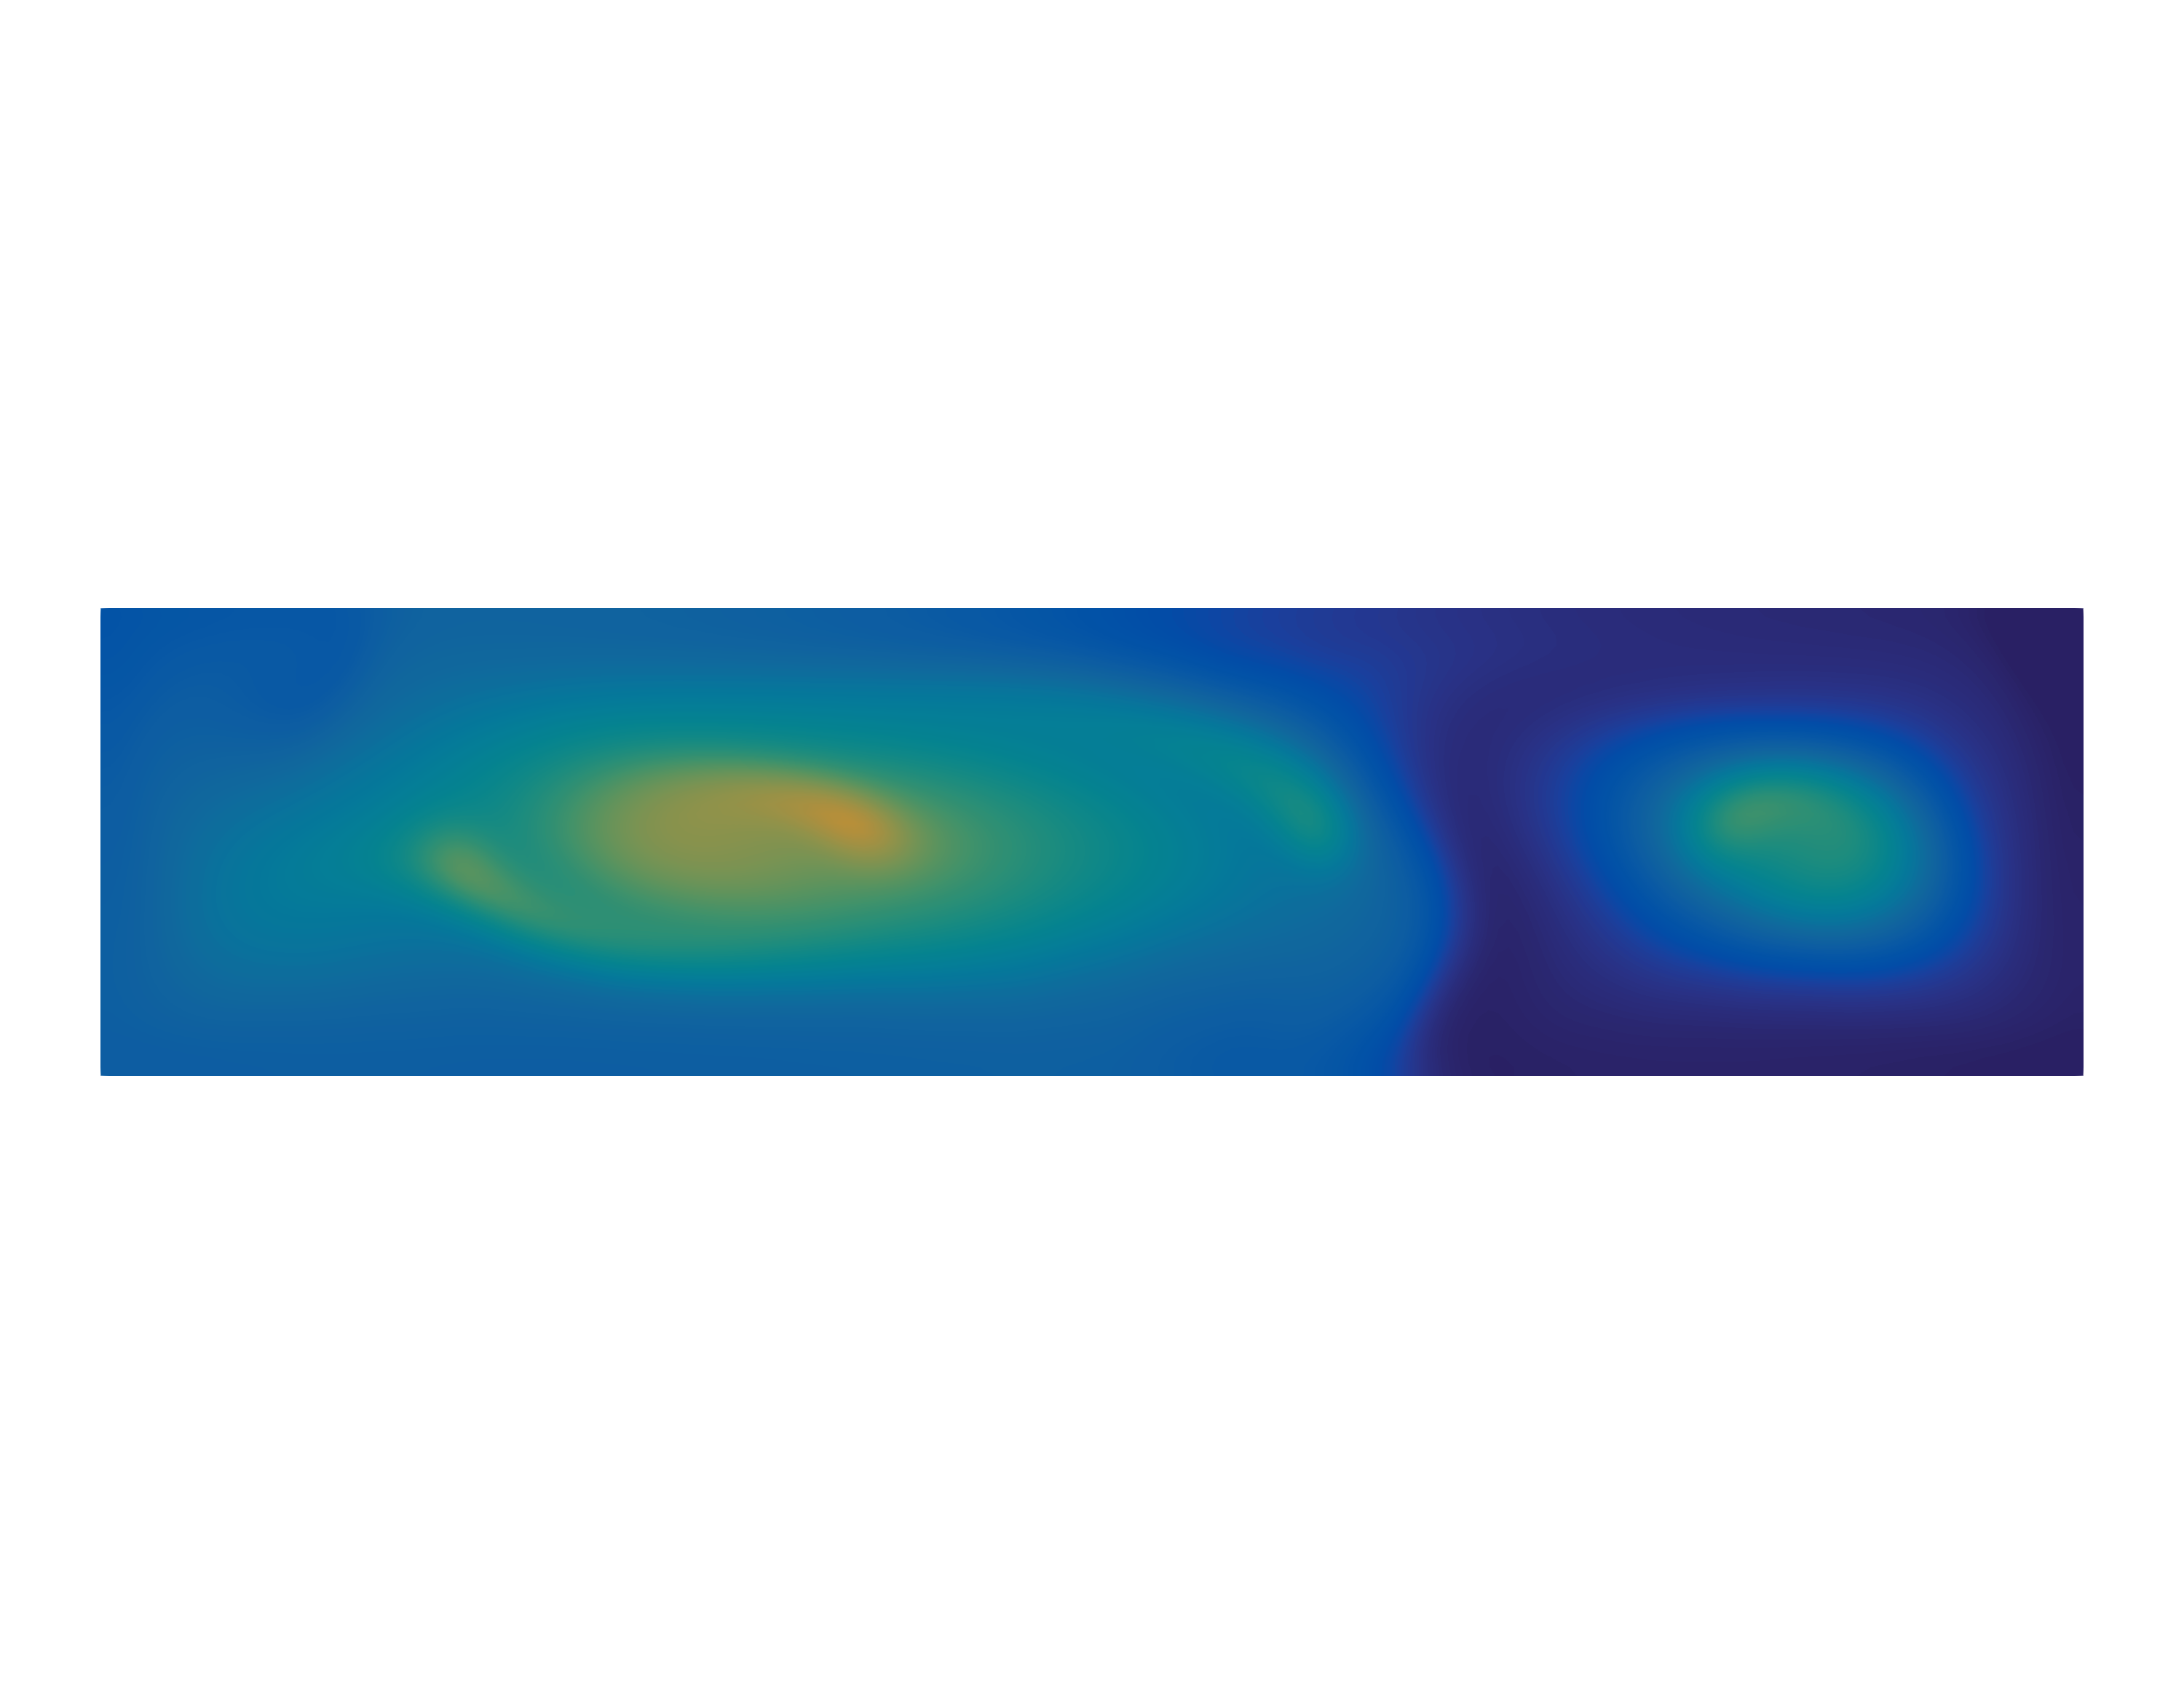
\includegraphics[width=0.99\textwidth]{../media/fourier/application/print/ab-0-1-concentration-harm-fc.png}
      \caption{Anode $(1,1)$ désactivée}
    \end{subfigure}

    \begin{subfigure}[t]{\textwidth}
      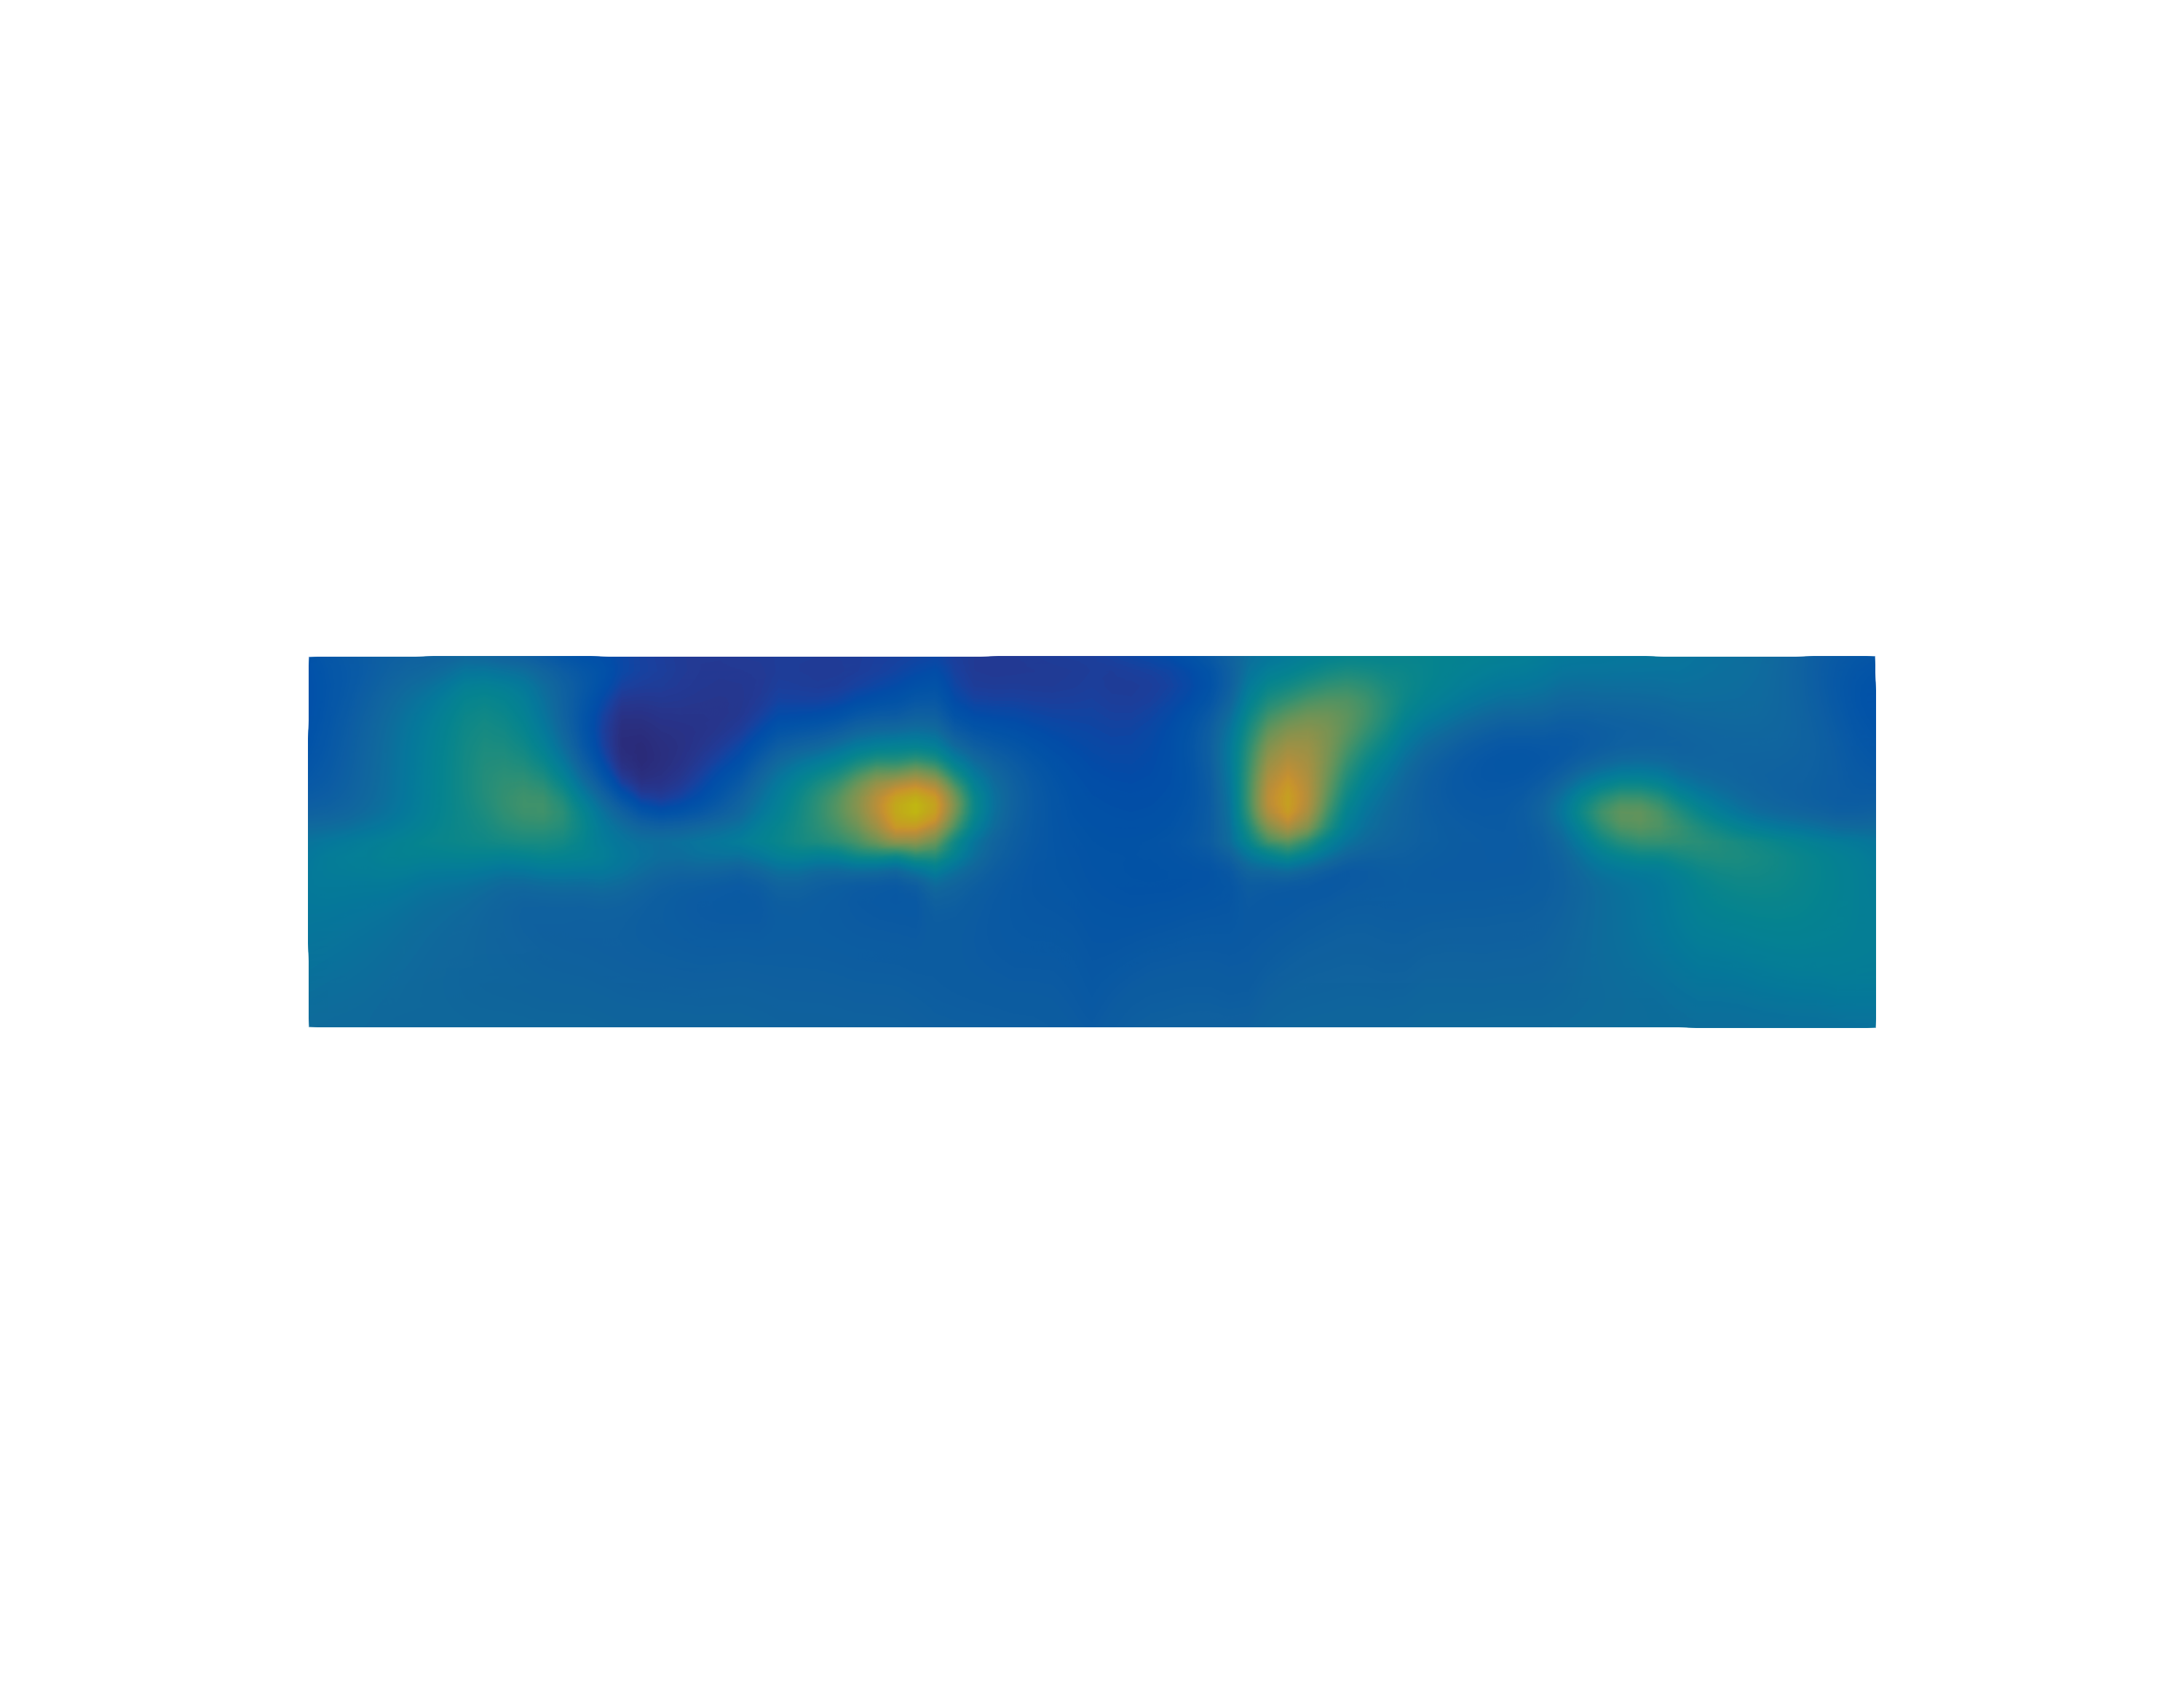
\includegraphics[width=0.99\textwidth]{../media/fourier/application/print/ab-0-2-concentration-acd.png}
      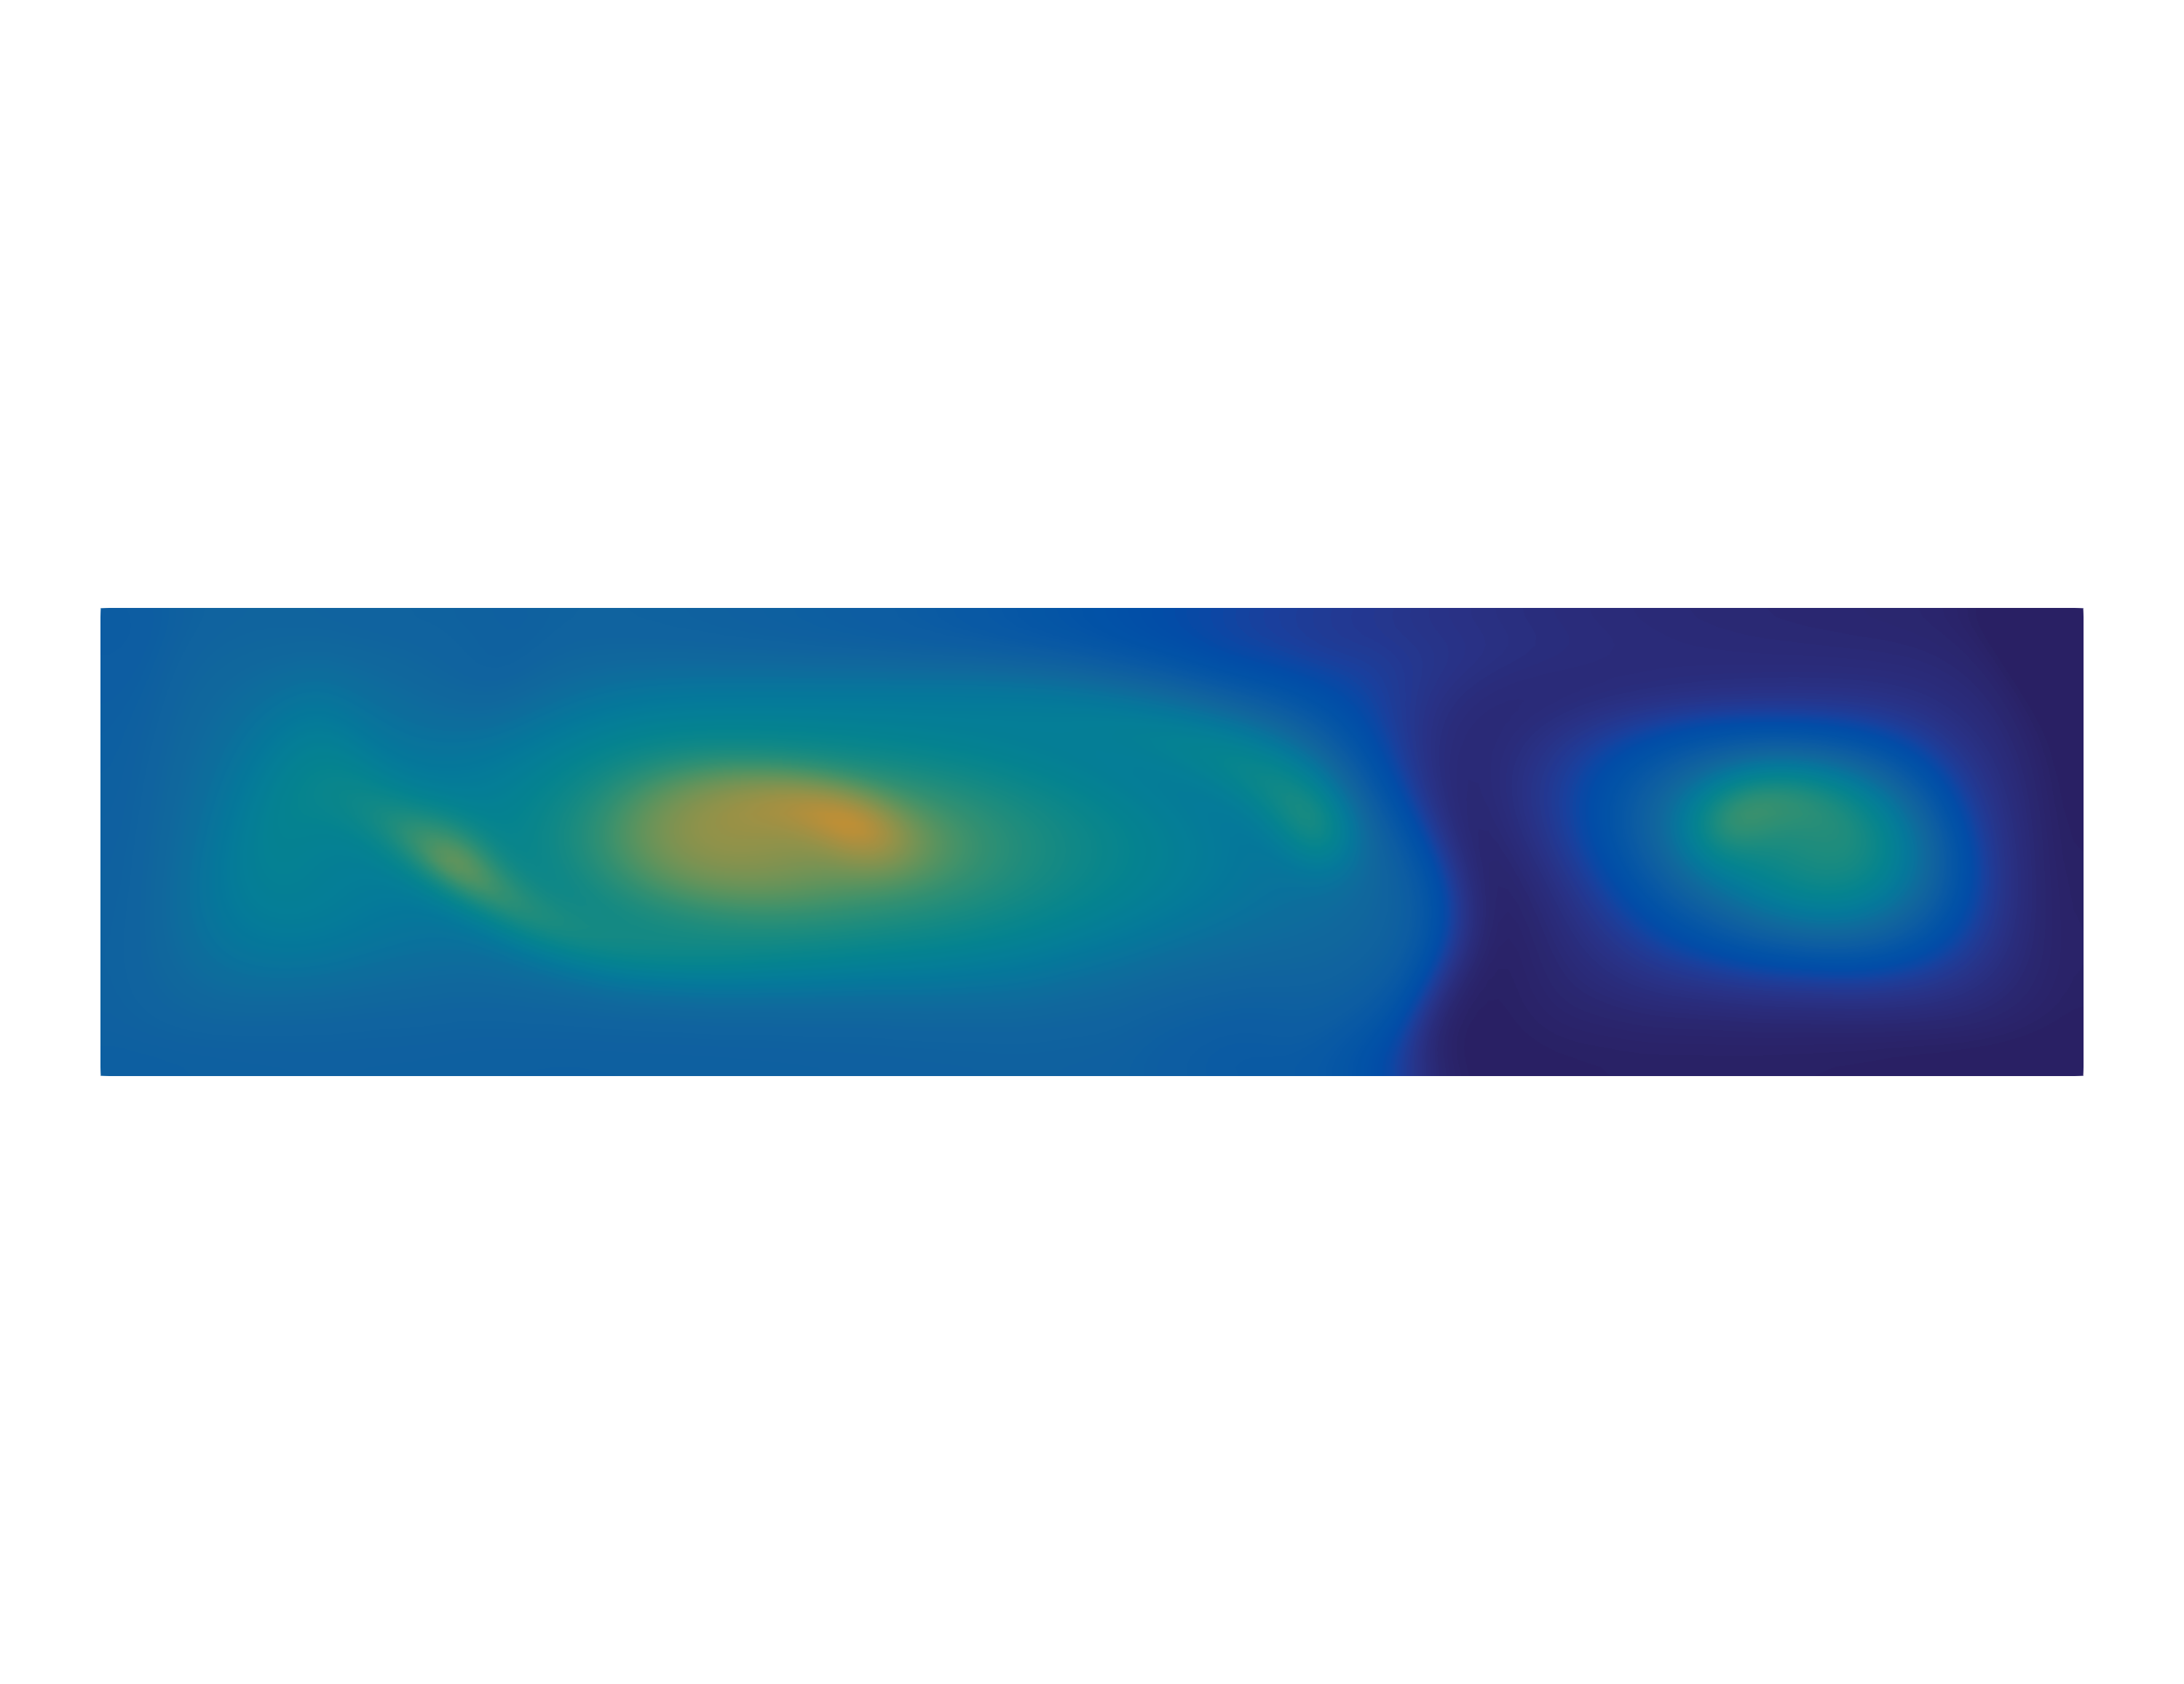
\includegraphics[width=0.99\textwidth]{../media/fourier/application/print/ab-0-2-concentration-harm-fc.png}
      \caption{Anode $(1,2)$ désactivée}
    \end{subfigure}

    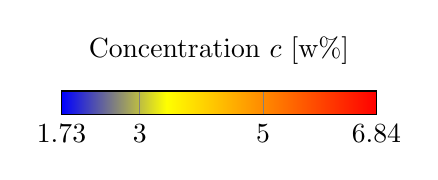
\begin{tikzpicture}
      \begin{axis}[
          colorbar,
          hide axis,
          scale only axis,
          height=0.1\textwidth,
          width=0.5\textwidth,
          colorbar horizontal,
          point meta min=1.73,
          point meta max=6.84,
          colorbar style={
            title=Concentration $c$ [w\%],
            width=4cm,
            height=0.3cm,
            xtick={1.73, 3.0, 5.0, 6.84},
            at={(0.3\textwidth,0.4cm)},
            anchor=north
          }
        ]
        \addplot [] coordinates {(0,0)};
        \node (myfirstpic) at (0,0) {};
      \end{axis}
    \end{tikzpicture}

    \caption{Champ de concentration $c_h^\mathrm{S3D}$ dans l'ACD de
      la cuve AP32 (haut), et $c_h^\mathrm{SF}$ sur le plan
      $x_3 = \thickness / 2$ (bas). La force $f$ utilisée
      pour le calcul de $u_h^\mathrm{SF}$  est construite à
      partir de $f^0$, qui est annulée sous l'anode désactivée.}

    \label{fig:harmonic-concentration-comp-fc}
  \end{center}
\end{figure}

\begin{figure}[h!]
  \begin{center}
    \begin{subfigure}[t]{\textwidth}
      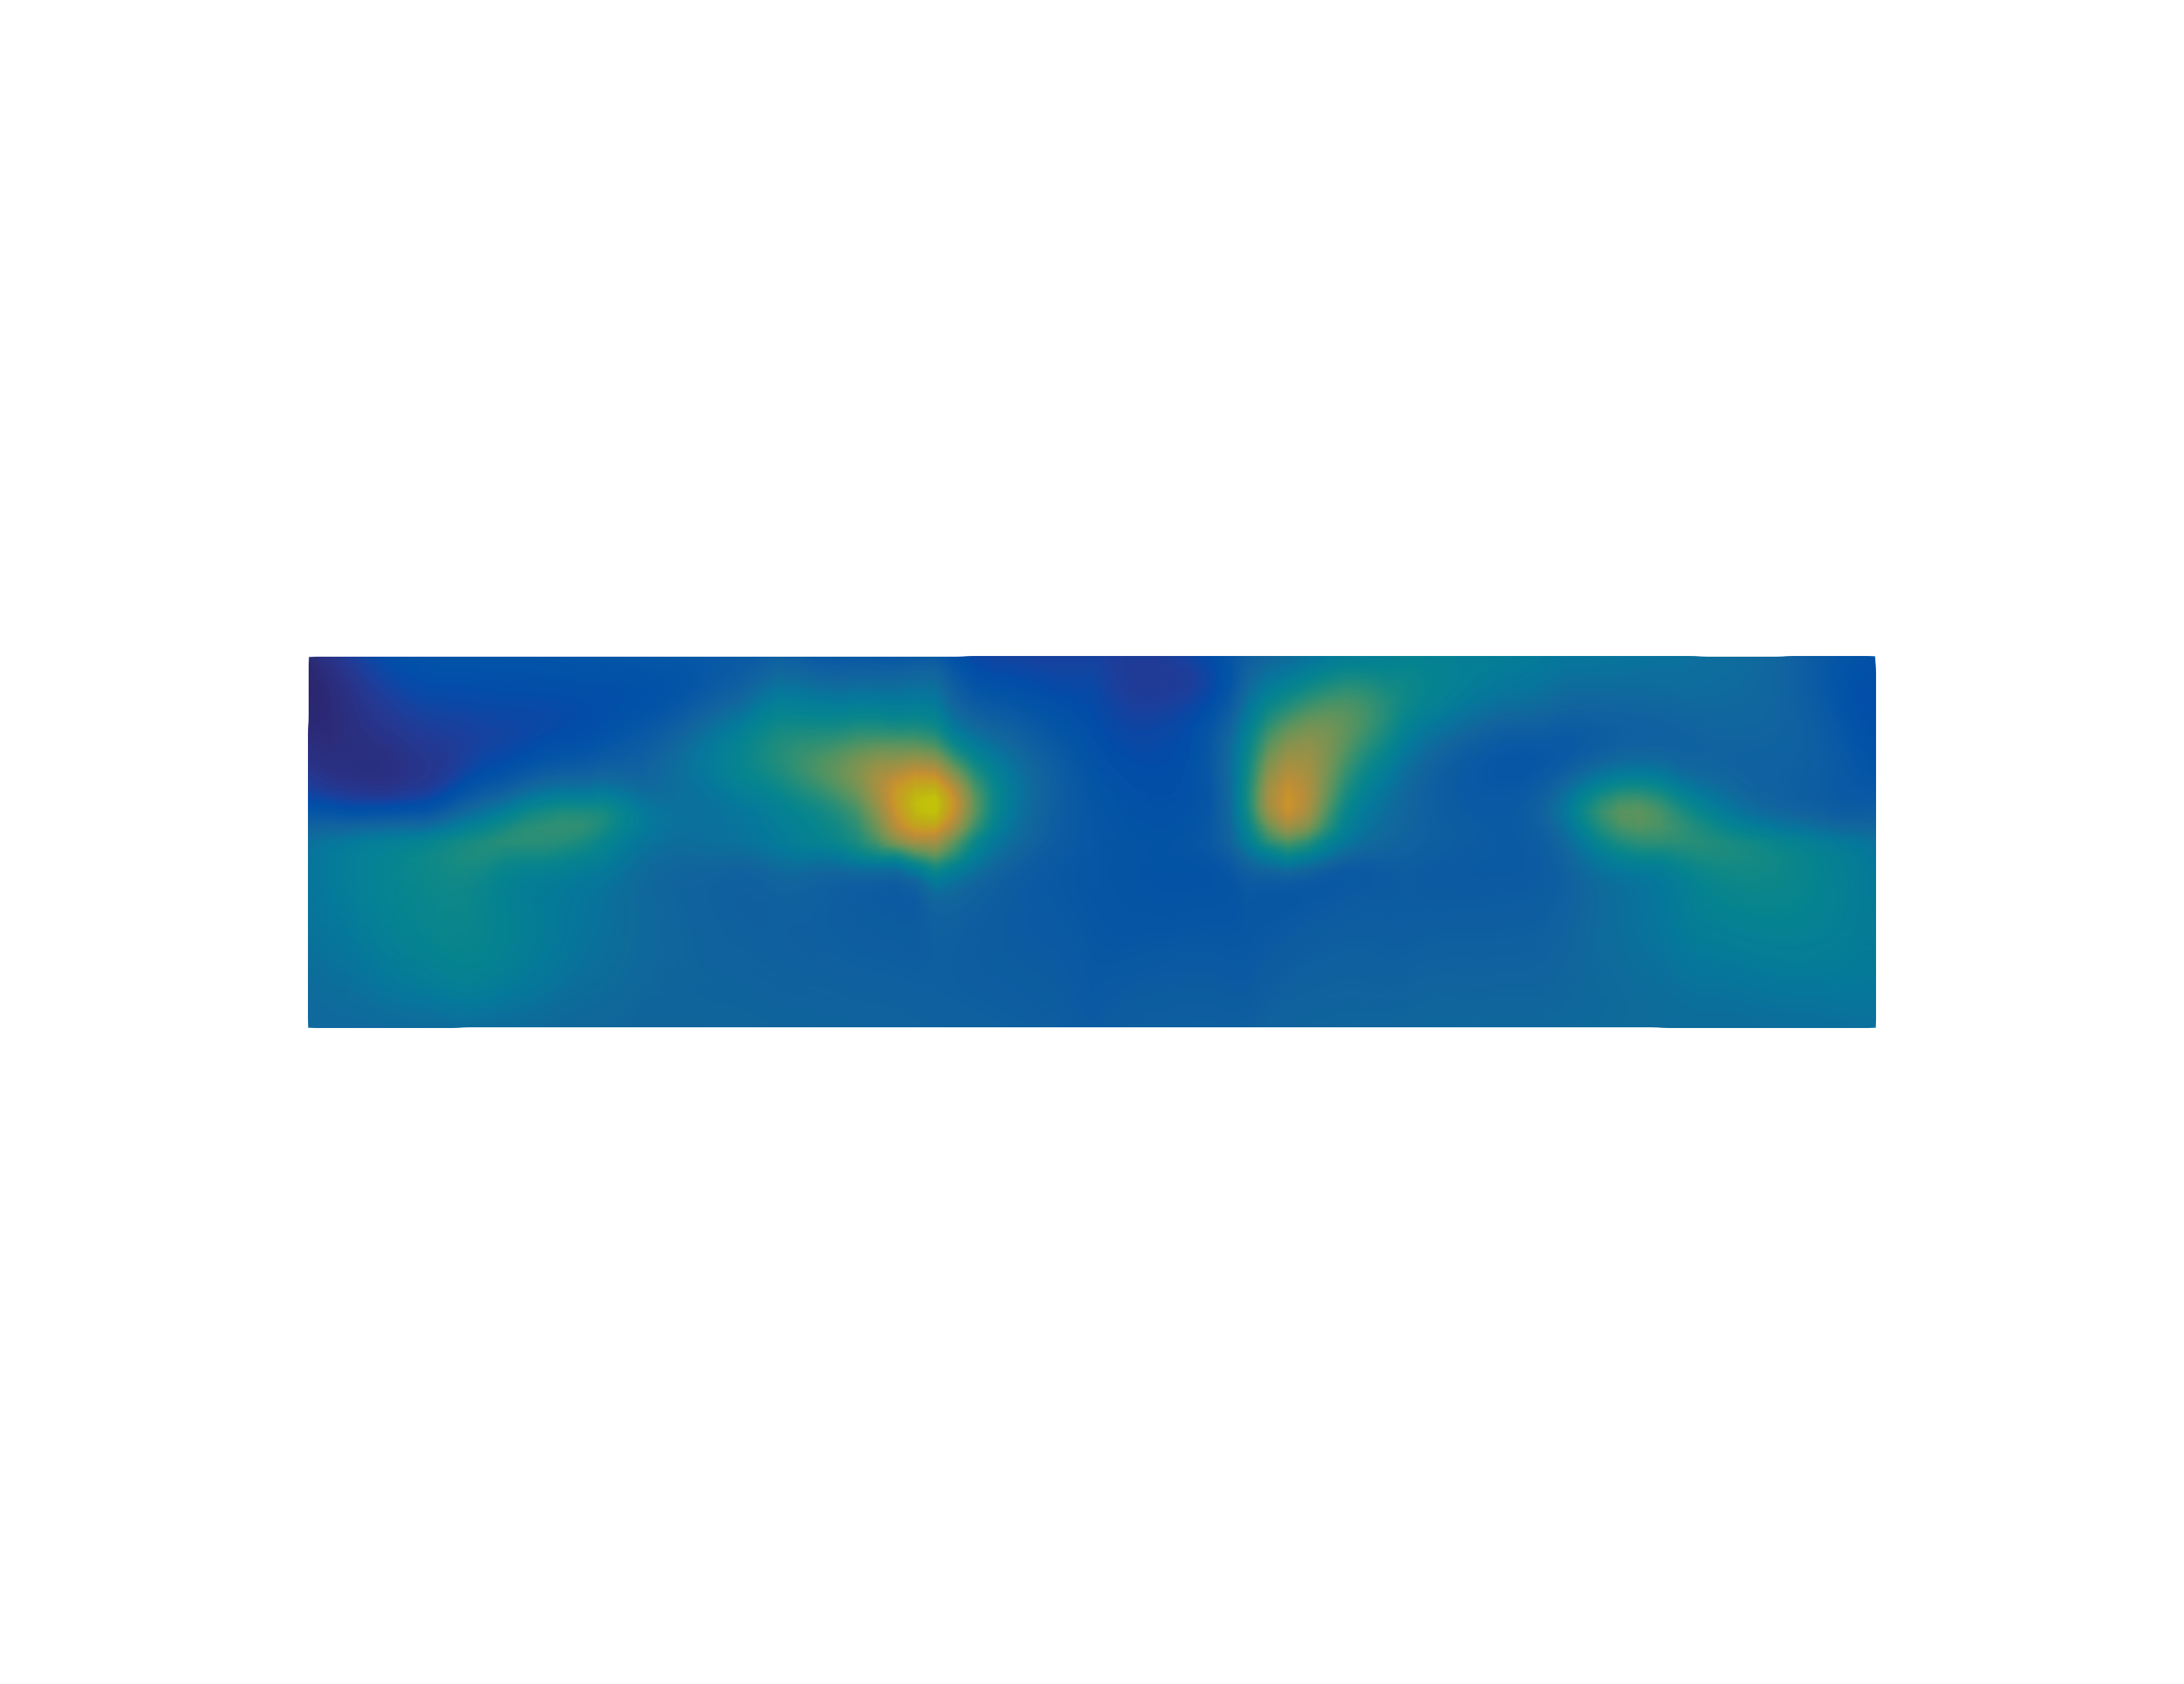
\includegraphics[width=0.99\textwidth]{../media/fourier/application/print/ab-1-1-concentration-acd.png}
      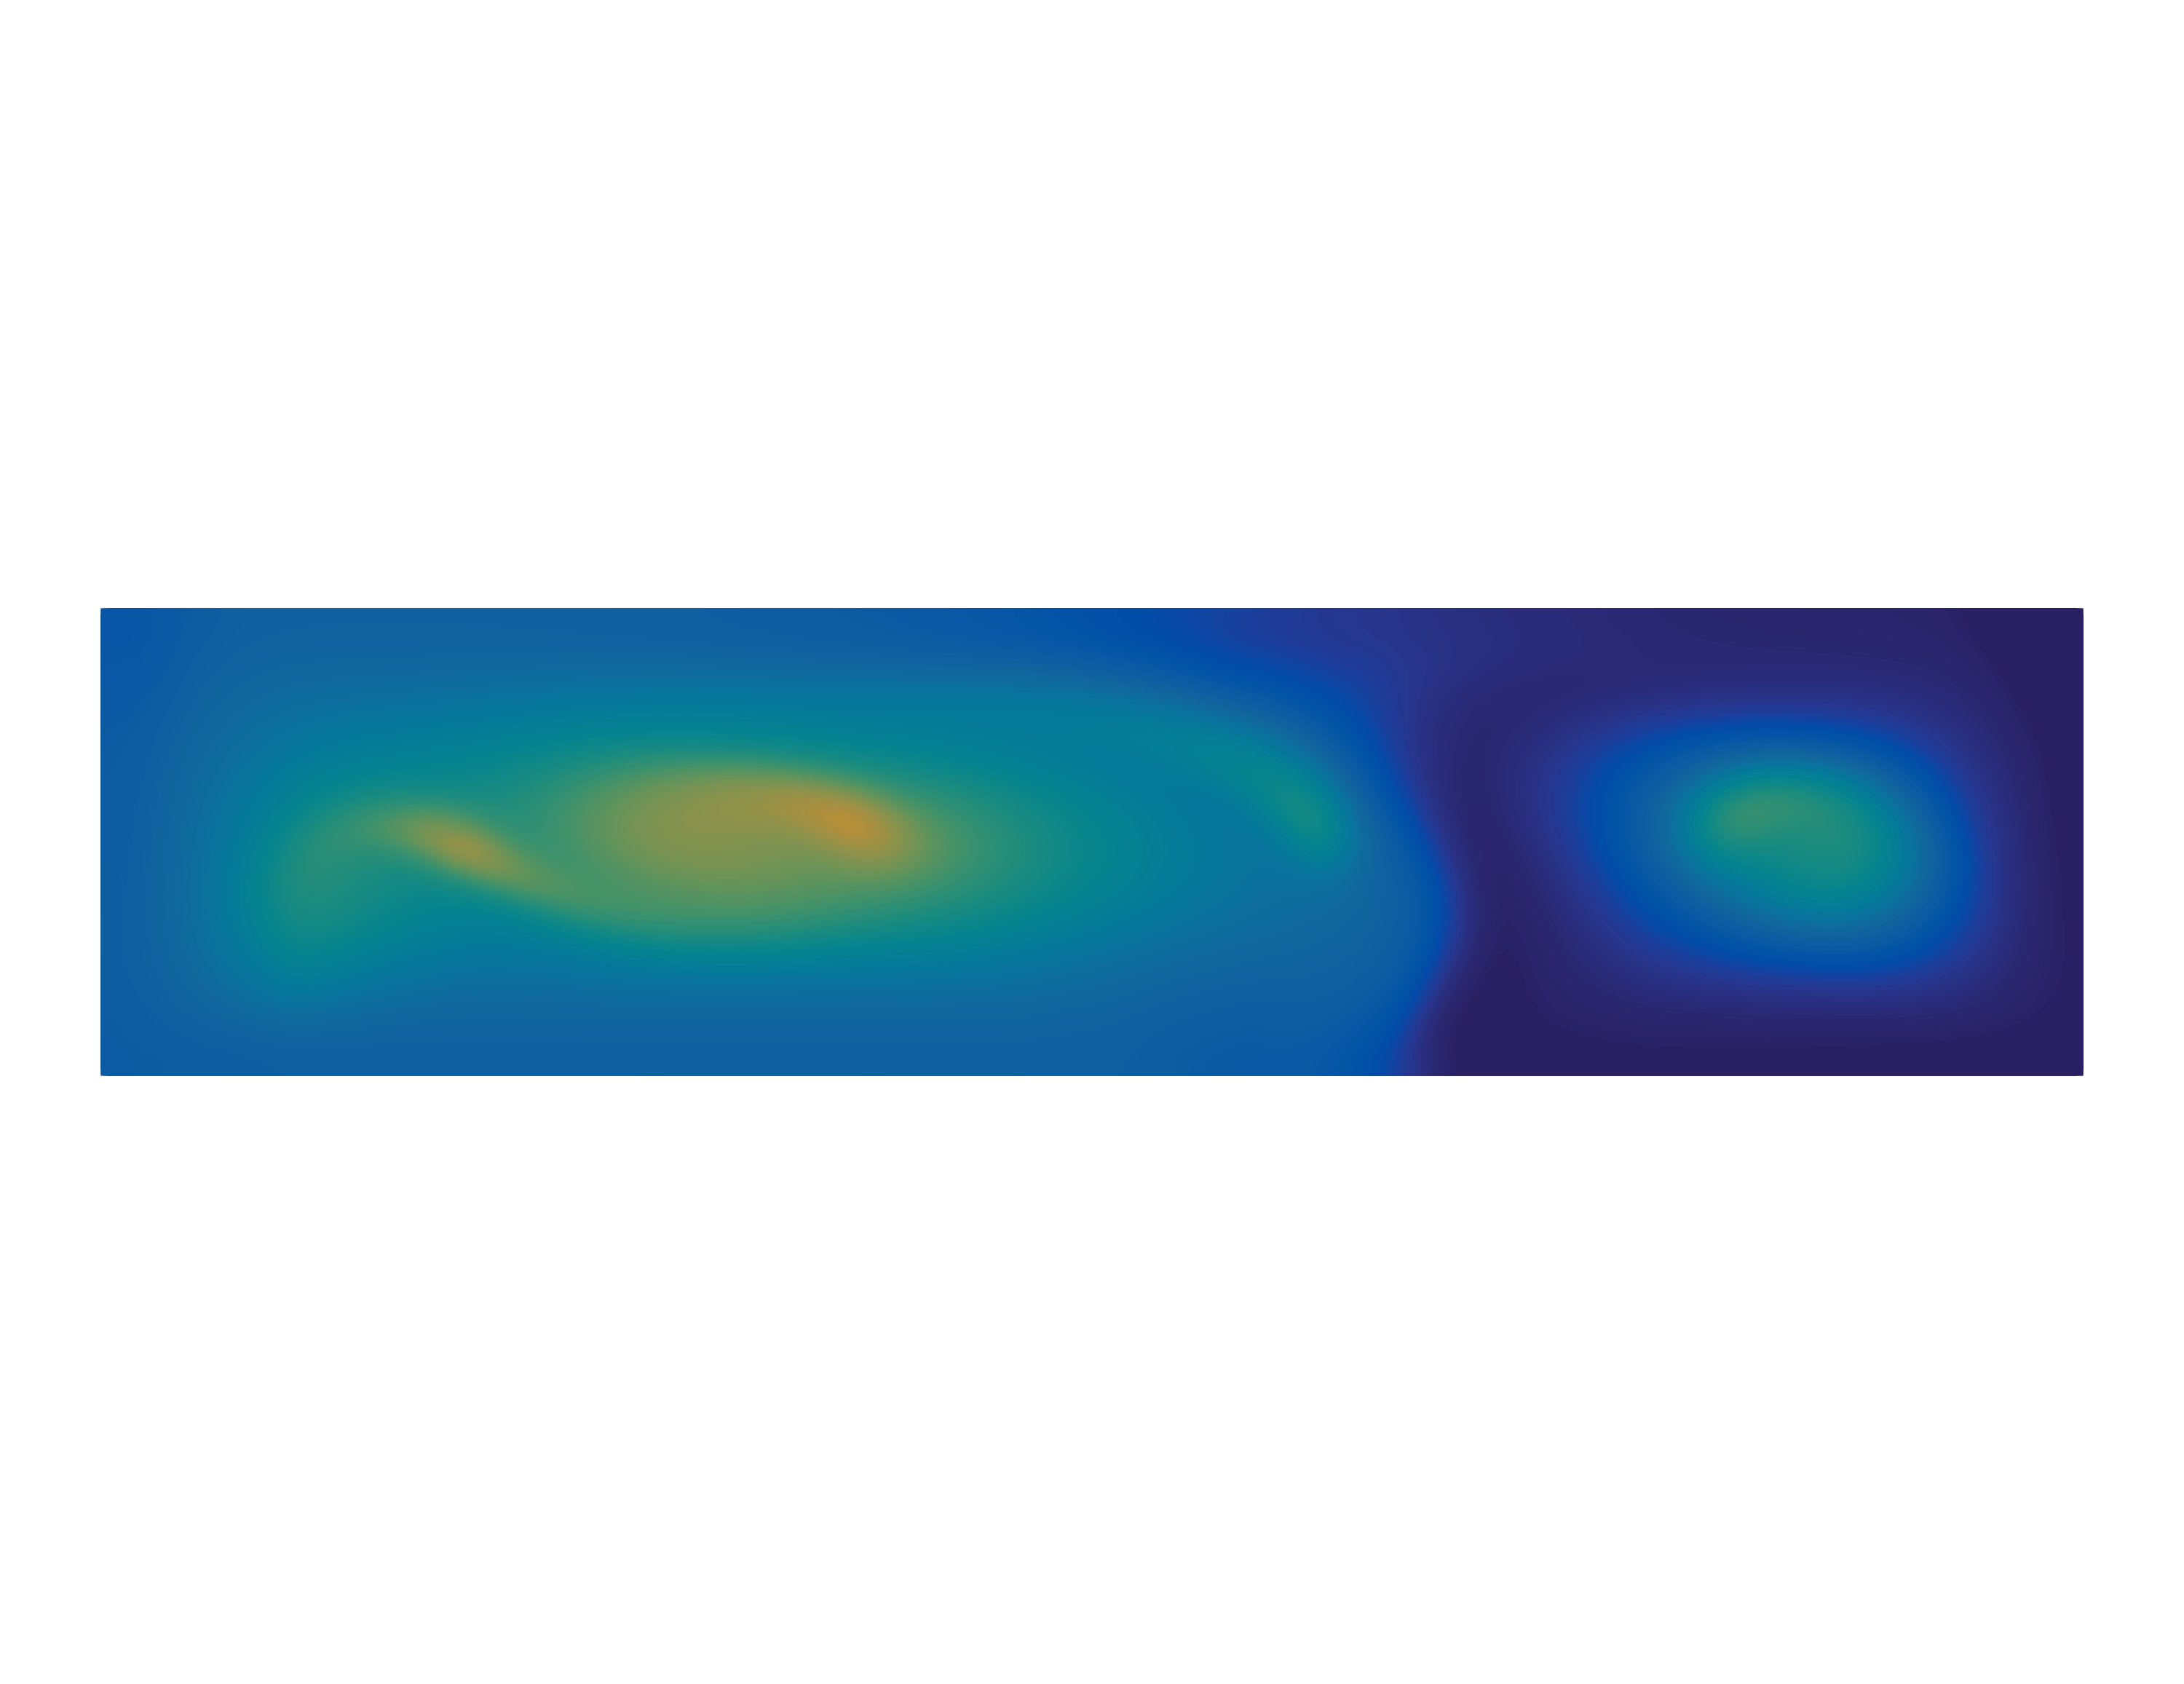
\includegraphics[width=0.99\textwidth]{../media/fourier/application/print/ab-1-1-concentration-harm-fc.png}
      \caption{Anode $(2,1)$ désactivée}
    \end{subfigure}

    \begin{subfigure}[t]{\textwidth}
      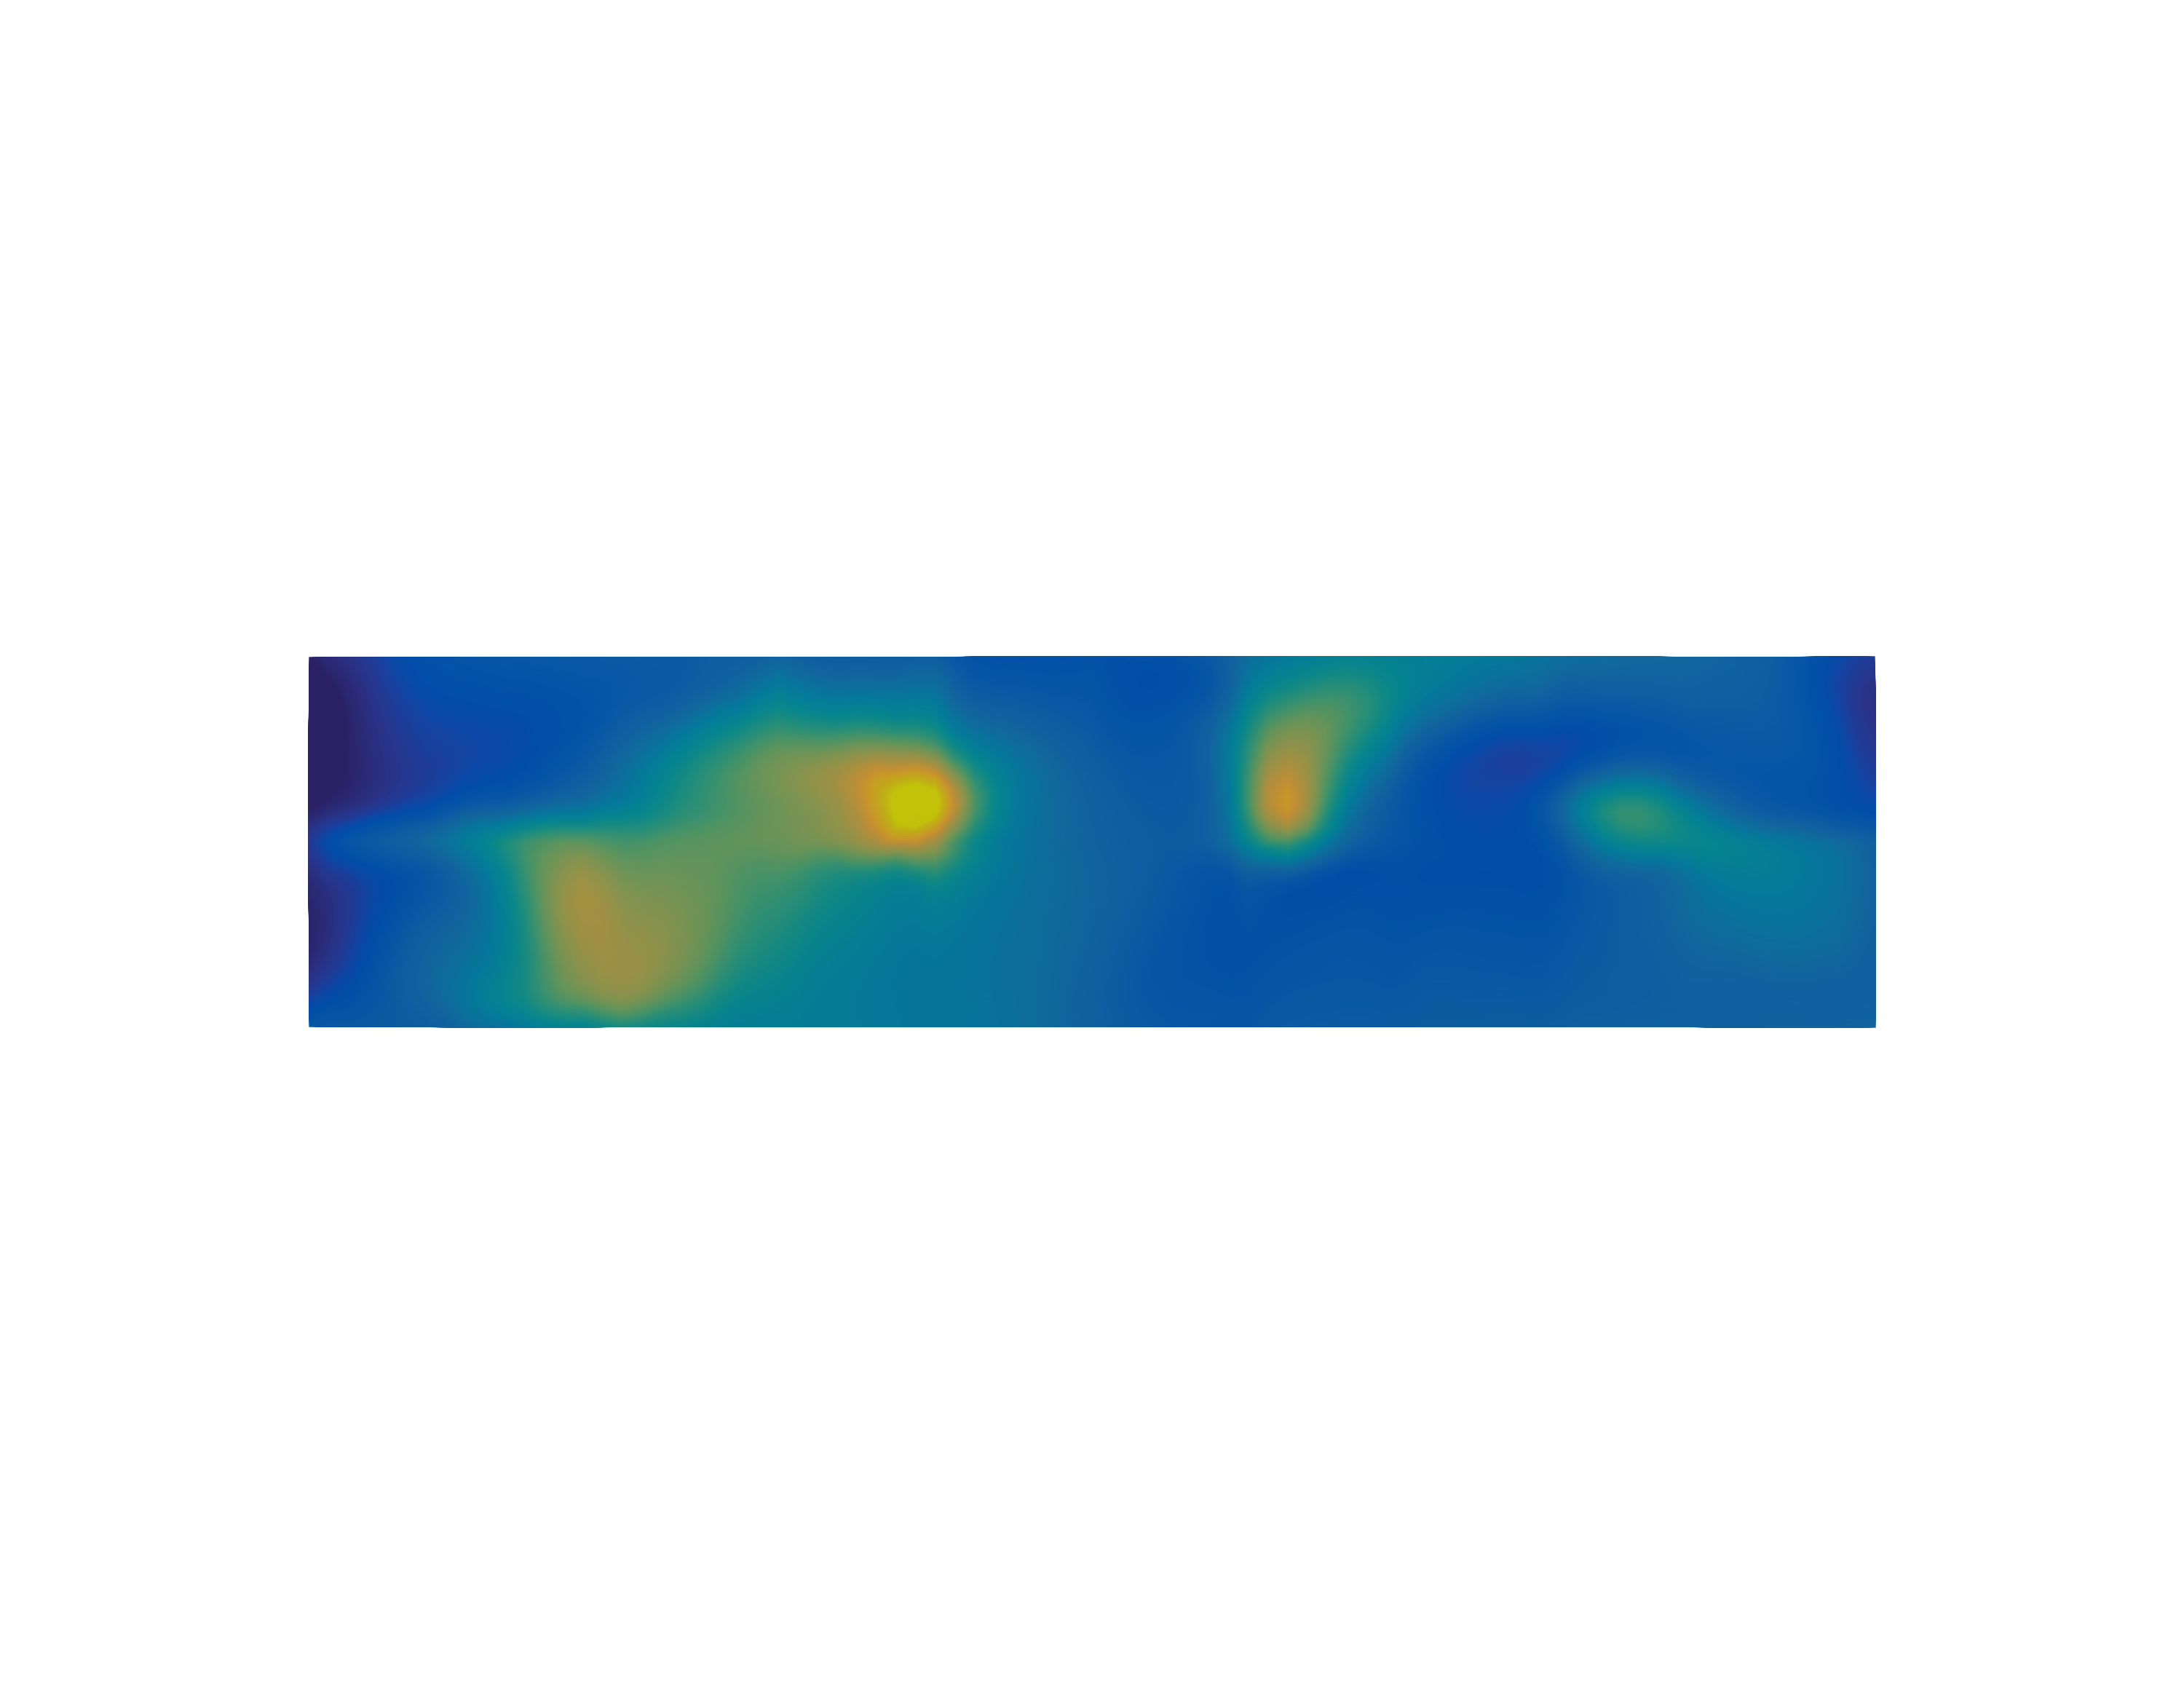
\includegraphics[width=0.99\textwidth]{../media/fourier/application/print/ab-1-2-concentration-acd.png}
      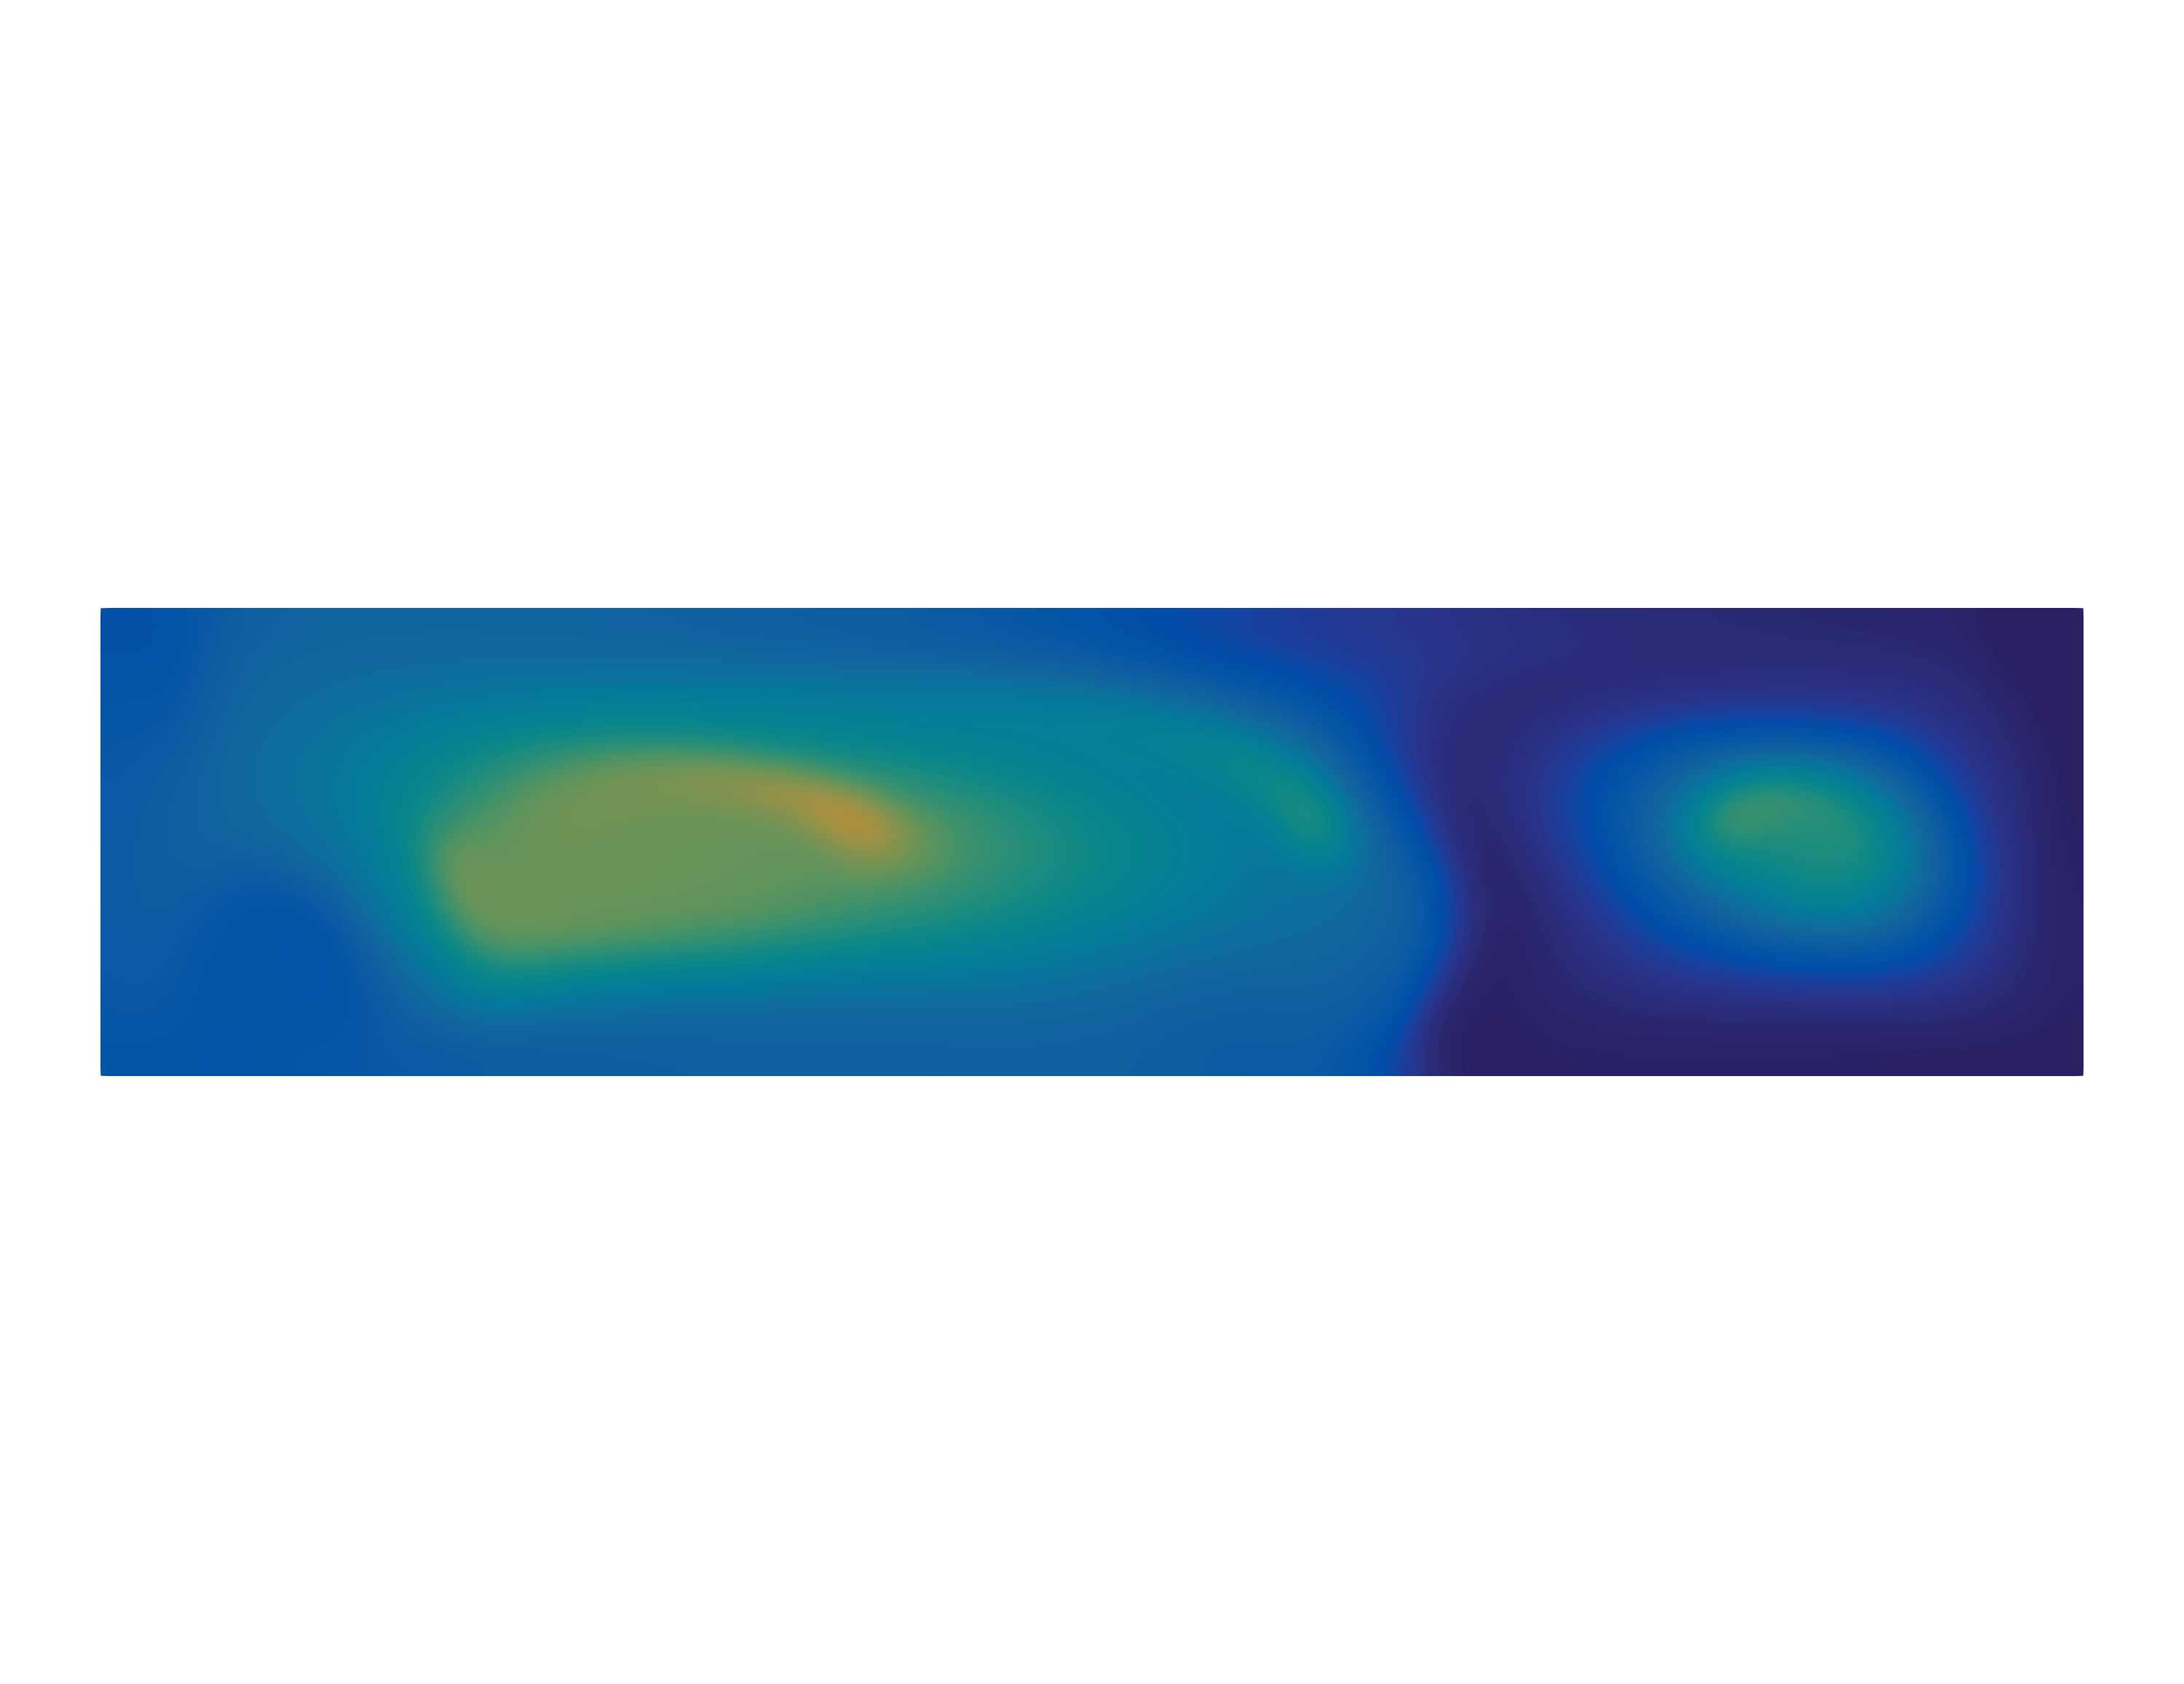
\includegraphics[width=0.99\textwidth]{../media/fourier/application/print/ab-1-2-concentration-harm-fc.png}
      \caption{Anode $(2,2)$ désactivée}
    \end{subfigure}

    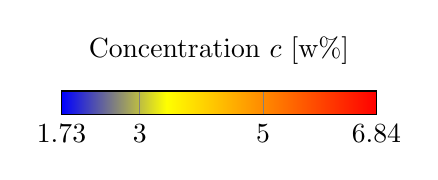
\begin{tikzpicture}
      \begin{axis}[
          colorbar,
          hide axis,
          scale only axis,
          height=0.1\textwidth,
          width=0.5\textwidth,
          colorbar horizontal,
          point meta min=1.73,
          point meta max=6.84,
          colorbar style={
            title=Concentration $c$ [w\%],
            width=4cm,
            height=0.3cm,
            xtick={1.73, 3.0, 5.0, 6.84},
            at={(0.3\textwidth,0.4cm)},
            anchor=north
          }
        ]
        \addplot [] coordinates {(0,0)};
        \node (myfirstpic) at (0,0) {};
      \end{axis}
    \end{tikzpicture}

    \caption{Champ de concentration $c_h^\mathrm{S3D}$ dans l'ACD de la
      cuve AP32 (haut), et $c_h^\mathrm{SF}$ sur le plan $x_3 = \thickness
      / 2$ (bas). La force $f$ utilisée pour le calcul de
      $u_h^\mathrm{SF}$ est construite à partir de $f^0$, qui est annulée
      sous l'anode désactivée.}

    \label{fig:harmonic-concentration-comp-fc}
\end{center}
\end{figure}

\clearpage


\section{Conclusion}
\label{sec:fourier-conclusion}
Dans ce dernier chapitre, nous avons proposé une méthode numérique
pour calculer l'écoulement de fluides dans un domaine
$\Omega = \Lambda\times(0,\thickness)$ de $\mathbb R^3$, basée sur une
décomposition en harmoniques de Fourier des inconnues et des
méthodes d'éléments finis pour chaque coefficients des séries de
Fourier. Cette formulation nécessite d'imposer des conditions
d'adhérence sur les bords verticaux du domaine et des conditions de
glissement total sur les bords horizontaux.

Une caractésistique essentielle de cette méthode est de calculer une
approximation de l'écoulement tridimensionnel en résolvant une
série de problèmes bidimensionnels découplés les uns des autres. Cette
approche devient de plus en plus intéressante lorsque l'épaisseur du
domaine $\thickness$ s'approche de 0. En effet, on observe d'une part
que le temps CPU est essentiellement indépendent de $\thickness$, mais
en plus l'erreur d'approximation diminue lorsque $\thickness$
diminue. C'est un clair avantage par rapport à une méthode
d'éléments finis classiques basée sur un maillage tetraédrique. En
raison de la péjoration du conditionnement des matrice éléments
finis lorsque $\thickness$ tend vers 0, \ie, lorsque le rapport
d'aspect du maillage devient de plus en plus grand, la convergence des
méthodes iteratives devient de plus en plus lente. De plus, l'erreur
d'approximation tend a croître lorsque $\thickness$ diminue.

Cette méthode est donc bien adaptée au calcule d'écoulement de
fluides en couches minces, pour autant que les conditions aux limites
soient adaptées.

